\documentclass[11pt,a4paper,footinclude=true,headinclude=true,oneside]{scrbook} % KOMA-Script book

\usepackage[T1]{fontenc}                
\usepackage{lipsum}
\usepackage[linedheaders,manychapters,pdfspacing]{classicthesis} % ,manychapters
%\usepackage[osf]{libertine}
\usepackage{amsthm}

% [MQH]
\usepackage[paperwidth=6.3in, paperheight=9.45in]{geometry}
\usepackage[htt]{hyphenat}
% ,bindingoffset=0.5in, left=1.5cm, right=2cm

\clearscrheadfoot
\ohead{\rightmark}
\cfoot[\pagemark]{\pagemark}

%left=5em, right=6em
\usepackage{graphicx}
\usepackage{longtable}
\usepackage{listings}
% Source: https://tex.stackexchange.com/a/179956
\usepackage{xcolor}
\lstset{
    basicstyle=\ttfamily,
    numbers=left,
    keywordstyle=\color[rgb]{0.13,0.29,0.53}\bfseries,
    stringstyle=\color[rgb]{0.31,0.60,0.02},
    commentstyle=\color[rgb]{0.56,0.35,0.01}\itshape,
    numberstyle=\footnotesize,
    stepnumber=1,
    numbersep=5pt,
    backgroundcolor=\color[RGB]{248,248,248},
    showspaces=false,
    showstringspaces=false,
    showtabs=false,
    tabsize=2,
    captionpos=b,
    breaklines=true,
    breakatwhitespace=true,
    breakautoindent=true,
    escapeinside={\%*}{*)},
    linewidth=\textwidth,
    basewidth=0.5em,
}

\begin{document}
    \title{A Journey in Creating an Operating System Kernel}
    \subtitle{The 539kernel Book}
    \author{Mohammed Q. Hussain}
    \date{November 2022}
    
    \maketitle
    
    \newpage
    \thispagestyle{plain}
    \mbox{}

	\tableofcontents 
	
    \newpage
    \thispagestyle{plain}
    \mbox{}
    
	\chapter*{Introduction}\label{introduction}

In about 17 years ago writing an operating system's kernel was kind of a
dream for me. Before 2 years of that time I just started my journey with
the wonderful world of computer science through learning programming for
web which made me curios about the different aspects of computers and of
course one of the most interesting of those aspects is operating
systems. At that time I wasn't technically ready yet to write an
operating system kernel, so, a number of experiments to achieve that
goal failed. After these trials, many years passed, I learned a lot
through these years and tackled a number of other system software (such
as compilers, virtual machines and assemblers) to learn how they work
and even implemented some too simple versions of them to make sure that
I've understand their concepts. In 2017 I asked myself, why don't I
implement a simple operating system kernel and achieve one of the oldest
thing in my to-do list which was a kind of dream for me? ``Fine, but how
to make it a useful project for people?'' that's what I told myself as a
response. Going through this journey was interesting for me to learn
more, but I also wanted to make something that's useful for someone
other than me, and at that moment the idea of this book was born. At
that time, I was working on my Master's degree, so I didn't have enough
time to work on this project and that's made me to defer the work on it
until the late of 2019 and after a lot of torture (sorry! dedication?)
this book is finally here.

In this book we are going to start a journey of creating a kernel I
called 539kernel which is a really simple x86 32-bit operating system
kernel that supports multitasking, paging and has its own filesystem. I
wrote 539kernel for this book and made it as simple as possible, so,
anyone would like to learn about operating system kernels can use
539kernel to start. Due to that, some of you may notice that some part
of 539kernel code is written in a naive way, while writing 539kernel I
focused on the readability and easiness of the code instead of the
efficiency. Through this journey your are going to learn a lot about the
basics of operating systems, their kernels and of course the platform
that is going to run 539kernel that we will create together, I mean by
the platform the processors that use x86 architecture. For those who
don't know, an operating system kernel is the core of any operating
system and its job is managing the computer hardware and resources,
distribute these resources for the running programs and provide many
services for those programs to make it easy for them the work with these
resources and hardware.

This book requires a knowledge in \lstinline!C! programming language,
you know; the basics, its syntax, defining variable and functions,
pointers and so on, you don't need to be a master on \lstinline!C!'s
libraries for example. The compiler used to create and test 539kernel is
GNU GCC \lstinline!7.5!. Also, assembly programming language will be
used, but the book doesn't require a knowledge in this language, every
aspect you need to learn about x86 assembly in order to create 539kernel
will be explained in this book. We will use \lstinline!NASM! assembler
for our assembly code and we will use GNU Make to build our kernel,
also, QEMU or Bochs will be used as an emulator to test our work through
this journey. All these three tools will be discussed in chapter
\ref{ch-bootloader} but you need to set them up in your machine. The
full source code of 539kernel is available in GitHub
(\url{https://github.com/MaaSTaaR/539kernel}), there are two directories
in the root directory, \lstinline!src/! is one that contains the last
version of 539kernel, that is, when you finish this book, the code that
you will get will be same as the one in \lstinline!src/!. The directory
\lstinline!evolution_by_versions/! contains the version of 539kernel
while it's under development through the different chapters in this
book. Finally, I hope that you enjoy reading this book and I would be
more than happy to hear your feedback and to help me in spreading this
book which is available freely in (\url{http://539kernel.com}).

\section*{Acknowledgment}\label{acknowledgment}

I would like to thank Dr.~Hussain Almohri \footnote{\url{https://almohri.io/}}
for his kind acceptance to read this book before its release and for his
encouragement, feedback and discussions that really helped me. Also, I
would like to thank my friends Anas Nayfah, Ahmad Yassen, DJ., Naser
Alajmi and my dearest niece Eylaf for their kind support.

\begin{center}\rule{0.5\linewidth}{\linethickness}\end{center}

Mohammed Q. Hussain
(\href{mailto:mqh@539kernel.com}{\nolinkurl{mqh@539kernel.com}})

16 November 2022

Kuwait

	
	\newpage
    \thispagestyle{plain}
    \mbox{}
    
	\chapter{Chapter 1: Let's Start with the
Bootloader}\label{ch-bootloader}

\section{Introduction}\label{introduction}

The first piece to start with when writing an operating system's kernel
is the \emph{boot loader} which is the code that is responsible for
loading the main kernel from the disk to the main memory so the kernel
can be executed. Before getting started in the details of the boot
loader and all other parts of the kernel, we need to learn a little bit
about the tools (e.g.~compilers and programming languages) that we will
use in our journey of creating a kernel. In this chapter, we start with
an overview on the tools and their basics and then we start in writing a
boot loader.

\section{x86 Assembly Language
Overview}\label{x86-assembly-language-overview}

To build a boot loader, we need to use assembly language, also, there
are some parts of an operating system kernel that cannot be written in a
high-level language and assembly language should be used instead as you
will see later in this book, therefore, a basic knowledge of the target
architecture assembly is required, in our case, the target architecture
of our kernel is x86.

The program that takes a source code which is written in assembly
language and transforms this code to the machine language is known as
\emph{assembler} \footnote{While the program that transforms the source
  code which is written in high-level language such as C to machine code
  is known as \emph{compiler}.}. There are many assemblers available for
x86 but the one that we are going to use is Netwide Assembler (NASM).
However, the concepts of x86 assembly are the same, they are tight to
the architecture itself, also the instructions are the same, so if you
grasp the basics it will be easy to use any other assembler \footnote{Another
  popular open-source assembler is GNU Assembler (GAS). One of main
  differences between NASM and GAS that the first uses Intel's syntax
  while the second uses AT\&T syntax.} even if it uses other syntax than
NASM. Don't forget that the assembler is just a tool that helps us to
generate an executable x86 machine code out of an assembly code, so, any
suitable assembler that we use to reach our goal will be enough.

In this section I don't aim to examine the details of x86 or NASM, you
can consider this section as a quick start on both x86 and NASM, the
basics will be presented to make you familiar with x86 assembly
language, more advanced concepts will be presented later when we need
them. If you are interested in x86 assembly for its own sake, there are
multiple online resources and books that explain it in details.

\subsection{Registers}\label{registers}

In any processor architecture, and x86 is not an exception, a register
is a small memory inside the processor's chip. Like any other type of
memories (e.g.~RAM), we can store data inside a register and we can read
data from it, the registers are too small and too fast. The processor
architecture provides us with multiple registers. In x86 there are two
types of registers: general purpose registers and special purpose
registers. In general purpose registers we can store any kind of data we
want, while the special purpose registers are provided by the
architecture for some specific purposes, we will encounter the second
type later in our journey of creating 539kernel.

x86 provides us with eight general purpose registers and to use them in
order to read from or write to them we refer to them by their names in
assembly code. The names of these registers are: \lstinline!EAX!,
\lstinline!EBX!, \lstinline!ECX!, \lstinline!EDX!, \lstinline!ESI!,
\lstinline!EDI!, \lstinline!EBP!, and \lstinline!ESP!. While the
registers \lstinline!ESI!, \lstinline!EDI!, \lstinline!EBP! and
\lstinline!ESP! are considered as general purpose registers in x86
architecture \footnote{According to Intel's manual.}, we will see later
that they store some important data in some cases and it's better to use
them carefully if we are forced to.

The size of each one of x86's general purpose registers is
\lstinline!32! bits (\lstinline!4! bytes) and due to that, they are
available only on x86 processors that supports \lstinline!32-bit!
architecture \footnote{Also they are available on \textbf{64-bit} x86
  CPUs such as Core i7 for instance.} such as Pentium 4 for instance.
These \lstinline!32-bit! registers are not available on x86 processors
that support only \lstinline!16-bit! architecture or lower, so, for
example, you can't use the register \lstinline!EAX! in Intel 8086
because it is a \lstinline!16-bit! x86 processor and not
\lstinline!32-bit!.

In old days, when \lstinline!16-bit! x86 processors were dominant,
assembly programmers used the registers \lstinline!AX!, \lstinline!BX!,
\lstinline!CX! and \lstinline!DX! and each one of them is of size
\lstinline!16! bits (\lstinline!2! bytes), but when \lstinline!32-bit!
x86 processors came, these registers have been extended to have the size
\lstinline!32-bit! and their names were changed to \lstinline!EAX!,
\lstinline!EBX!, \lstinline!ECX! and \lstinline!EDX!. The first letter
\lstinline!E! of the new names means \emph{extended}. However, the old
names are still usable in \lstinline!32-bit! x86 processors and they are
used to access and manipulate the first \lstinline!16! bits of the
corresponding register, for instance, to access the first \lstinline!16!
bits of the register \lstinline!EAX!, the name \lstinline!AX! can be
used. Furthermore, the first \lstinline!16! bits of these registers can
be divided into two parts and each one of them is of size \lstinline!8!
bits (\lstinline!1! bytes) and has its own name that can be referred to
in the assembly code. The first \lstinline!8! bits of the register are
called the \emph{low} bits, while the second \lstinline!8! bits are
called the \emph{high} bits.

Let's take one of these register as an example:\lstinline!AX! register
is a \lstinline!16-bit! register which is a part of the bigger
\lstinline!32-bit! \lstinline!EAX! register in \lstinline!32-bit!
architecture. \lstinline!AX! \footnote{Or in other words for
  \lstinline!32-bit! architecture: The first \lstinline!16! bits of
  \lstinline!EAX!.} is divided into two more parts, \lstinline!AL! for
the \textbf{l}ow \lstinline!8! bits as the second letter of the name
indicates and \lstinline!AH! for the \textbf{h}igh \lstinline!8! bits as
the second letter of the name indicates. The same division holds true
for the registers \lstinline!BX!, \lstinline!CX! and \lstinline!DX!,
figure \ref{fig:26012022_0} illustrates that division.

\begin{figure}
\centering
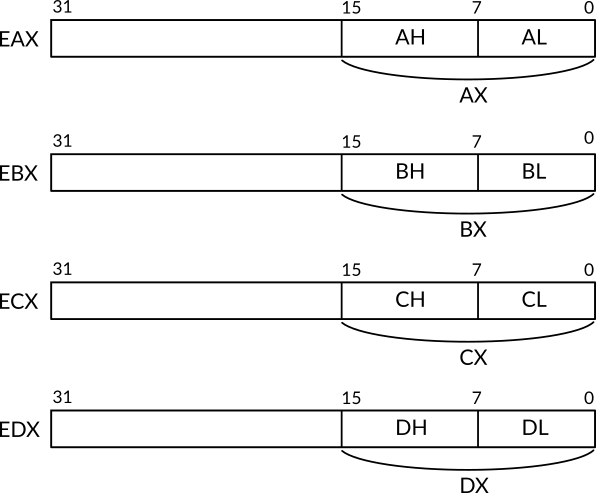
\includegraphics[width=0.50000\textwidth]{Figures/bootloader-ch/Fig26012022_0.png}
\caption{How the Registers \lstinline!EAX!, \lstinline!EBX!,
\lstinline!ECX! and \lstinline!EDX! are Divided in
x86}\label{fig:26012022_0}
\end{figure}

\subsection{Instruction Set}\label{instruction-set}

The processor's architecture provides the programmer with a bunch of
\emph{instructions} that can be used in assembly code. Processor's
instructions resemble functions \footnote{Or a procedure for people who
  work with Algol-like programming languages.} in a high-level languages
which are provided by the libraries, in our case, we can consider the
processor as the ultimate library for the assembly code. As with
functions in high-level programming languages, each instruction has a
name and performs a specific job, also, it can take parameters which are
called \emph{operands}. Depending on the instruction itself, the
operands can be a static value (e.g.~a number), a register name that the
instruction is going to fetch the stored value of it to be used or even
a memory location.

The assembly language is really simple. An assembly code is simply a
sequence of instructions which will be executed sequentially. The
following is an example of assembly code, don't worry about its
functionality right now, you will understand what it does eventually.

\begin{lstlisting}
mov ah, 0Eh
mov al, 's' 
int 10h
\end{lstlisting}

As you can see, each line starts with an instruction which is provided
to us by x86 architecture, in the first two lines we use an instruction
named \lstinline!mov! and as you can see, this instruction receives two
operands which are separated by a comma. In the current usage of this
instruction we can see that the first operand is a register name while
the second operand is a static value. The third line uses another
instruction named \lstinline!int! which receives one operand. When this
code is running, it will be executed by the processor sequentially,
starting from the first line until it finishes in the last line.

If you are interested on the available instructions on x86, there is a
four-volumes manual named ``Intel® 64 and IA-32 architectures software
developer's manual'' provided by Intel that explains each instruction in
details \footnote{\url{https://software.intel.com/en-us/articles/intel-sdm}}.

\subsubsection{\texorpdfstring{Assigning Values with
\texttt{mov}}{Assigning Values with mov}}\label{assigning-values-with-mov}

You can imagine a register as a variable in high-level languages. We can
assign values to a variable, we can change its old value and we can copy
its value to another variable. In assembly language, these operations
can be performed by the instruction \lstinline!mov! which takes the
value of the second operand and stores it in the first operand. You have
seen in the previous examples the following two lines that use
\lstinline!mov! instruction.

\begin{lstlisting}
mov ah, 0Eh
mov al, 's' 
\end{lstlisting}

Now you can tell that the first line copies the value \lstinline!0Eh! to
the register \lstinline!ah!, and the second line copies the character
\lstinline!s! to the register \lstinline!al!. The single quotation is
used in NASM to represent strings or characters and that's why we have
used it in the second line, based on that, you may noticed that the
value \lstinline!0Eh! is not surrounded by a single quotation though it
contains characters, in fact, this value isn't a string, it is a number
that is represented by hexadecimal numbering system and due to that the
character \lstinline!h! was put in the end of that value, that is,
putting \lstinline!h! in the end of \lstinline!0E! tells NASM that this
value is a hexadecimal number, the equivalent number of \lstinline!0E!
in the decimal numbering system, which we humans are using, is
\lstinline!14!, that is \lstinline!0E! and \lstinline!14! are the
exactly the same, but they are represented in two different numbering
system\footnote{Numbering systems will be discussed in more details
  later.}.

\subsection{NASM}\label{nasm}

Netwide Assembler (NASM) is an open-source assembler for x86
architecture which uses Intel's syntax of assembly language, the other
well-known syntax for assembly language is AT\&T syntax and, of course,
there are some differences between the two, the first syntax is used in
the official manuals of Intel. NASM can be used through command line to
assemble \footnote{The process of transforming an assembly source code
  to machine code is known as \emph{assembling}.} x86 assembly code and
generate the corresponding machine code. The basic usage of NASM command
is the following.

\begin{lstlisting}
nasm -f <format> <filename> [-o <output>]
\end{lstlisting}

The argument \lstinline!format! decides the binary format of the
generated machine code, the binary format will be discussed in more
details in a moment. The second argument is the \lstinline!filename! of
the assembly file that we would like to assemble, and the last option
and argument are optional, we use them if we want to specify a specific
name for the generated binary file, the default name will be same as the
filename with a different extension.

\subsubsection{Binary Format}\label{binary-format}

A \emph{binary format} is basically a specification which gives a
blueprint of how a binary file is organized, in other words, it
describes how a binary file is structured, in general there are multiple
parts in a binary file and a binary format can be used format them, the
machine code is one part of a binary file parts. Note that each
executable file uses some binary format to organize its content and to
make a specific operating system understands its content. There is no
difference between the programming languages in the matter of the binary
format \footnote{Of course the programming language should be a
  \emph{compiled} programming language such as C and Rust and not an
  \emph{interpreted} such as Python or a one that uses a virtual machine
  such as Java.} that will be used in the last output of the compiling
process, for example in Linux, if we create a software either by C, Rust
or assembly, the last executable result will be a binary file that is
formatted by using a binary format known as \emph{Executable and
Linkable Format} (ELF) which is the default in Linux. There are many
other binary formats, Mach-O is one example which is used by Mach-based
\footnote{Mach is an operating system's kernel which is well-known for
  using \emph{microkernel} design. It has been started as a research
  effort in Carnegie Mellon University in 1985. Current Apple's
  operating systems macOS and iOS are both based on an older operating
  system known as NeXTSTEP which used Mach as its kernel,}, another
example is Portable Executable (PE) which is used by Microsoft Windows.

Each operating system knows its own binary format well, and knows how a
binary file that uses this format is structured, and how to seek the
binary file to find the machine code that should be loaded into memory
and executed by the processor. For example, when you run an ELF
executable file in GNU/Linux system, the Linux kernel knows it is an ELF
executable file and assumes that it is organized in a specific way, by
using the specification of ELF, Linux kernel will be able to locate the
machine code of the software inside the ELF file and load it into memory
to be ready for execution.

In any binary format, one major part of the binary file that uses this
format is the machine code that has been produced by compiling or
assembling some source code, the machine code is specific to a processor
architecture, for example, the machine code that has been generated for
x64 \footnote{The x86 architecture that supports 64-bit.} cannot run on
x86. Because of that the binary files are distributed according to the
processor architecture which can run on, for example, GNU/Linux users
see the names of software packages in the following format
\lstinline!nasm_2.14-1_i386.deb!, the part \lstinline!i386! tells the
users that the binary machine code of this package is generated for
\lstinline!i386! architecture, which is another name for x86 by the way,
that means this package cannot be used in a machine that uses ARM
processor such as Raspberry Pi for example.

Due to that, to distribute a binary file of the same software for
multiple processor's architectures, a separate binary file should be
generated for each architecture, to solve this problem, a binary format
named \lstinline!FatELF! was presented. In this binary format, the
software machine code of multiple processor architectures are gathered
in one binary file and the suitable machine code will be loaded and run
based on the type of the system's processor. Naturally, the size of the
files that use such format will be bigger than the files that uses a
binary format that is oriented for one processor architecture. Due to
the bigger size, this type of binary formats is known as \emph{fat
binary}.

Getting back to the \lstinline!format! argument of NASM, if our goal of
using assembly language is to produce an executable file for Linux for
example, we will use \lstinline!elf! as a value for \lstinline!format!
argument. But we are working with low-level kernel development, so our
binary files should be flat and the value of \lstinline!format! should
be \lstinline!bin! to generate a \emph{flat binary} file which doesn't
use any specification, instead, in flat binary files, the output is
stored as is with no additional information or organization, only the
output machine language of our code. Using flat binary for bootloader
does make sense and that's because the code which is going to load
\footnote{Which is BIOS as we will see later.} our binary file doesn't
understand any binary format to interpret it and fetch the machine code
out of it, instead, the content of the binary file will be loaded to the
memory as is.

\section{GNU Make}\label{gnu-make}

GNU Make is a build automation tool. Well, don't let this fancy term
make you panic! the concept behind it is too simple. When we create a
kernel of an operating system \footnote{Or any software with any other
  compiled programming languages.} we are going to write some assembly
code and C code and both of them need to be assembled and compiled (for
the C code) to generate the machine code as binary files out of them.
With each time a modification is made in the source code, you need to
recompile (or reassemble) the code over and over again through writing
the same commands in the terminal in order to generate the last binary
output of your code. Beside the compiling and recompiling steps, an
important step needs to take place in order to generate the last output,
this operation is known as \emph{linking}, usually a programming project
contains multiple source files that call each other, compiling each one
of these files is going to generate a separate \emph{object file}
\footnote{An object file is a machine code of a source file and it is
  generated by the compiler. The object file is not an executable file
  and in our case at least it is used to be linked with other object
  files to generate the final executable file.} for each one, in linking
process these different object files are linked with each other to
generate one binary file out of these multiple object files, this last
binary file represents the program that we are writing.

These operations which are needed to generate the last binary file out
of the source code is known as \emph{building process}, which, as
mentioned earlier, involves executing multiple commands such as
compiling, assembling and linking. The building process a tedious job
and error-prone and to save our time (and ourselves from boredom of
course) we don't want to write all these commands over and over again in
order to generate the last output, we need an alternative and here where
GNU Make \footnote{And any other building automation tool.} comes to the
rescue, it \emph{automates} the \emph{building} process by gathering all
required commands in a text file known as \lstinline!Makefile! and once
the user runs this file through the command \lstinline!make!, GNU Make
is going to run these commands sequentially, furthermore, it checks
whether a code file is modified since the last building process or not,
if the case is that the file is not modified then it will not be
compiled again and the generated object file from the last building
process is used instead, which of course minimize the needed time to
finish the building process.

\subsection{Makefile}\label{makefile}

A \lstinline!makefile! is a text file that tells GNU Make what are the
needed steps to complete the building process of a specific source code.
There is a specific syntax that we should obey when writing
\lstinline!makefile!. A number of \emph{rules} may be defined, we can
say that a \lstinline!makefile! has a list of rules that define how to
create the executable file. Each rule has the following format:

\begin{lstlisting}[language=make]
target: prerequisites
    recipe
\end{lstlisting}

When we run the command \lstinline!make! without specifying a defined
target name as an argument, GNU Make is going to start with the first
rule in the \lstinline!makefile! only if the first rule's target name
doesn't start with dot, otherwise, the next rule will be considered. The
name of a target can be a general name or filename. Assume that we
defined a rule with the target name \lstinline!foo! and it's not the
first rule in \lstinline!makefile!, we can tell GNU Make to execute this
rule by running the command \lstinline!make foo!. One of well-known
convention when writing a \lstinline!makefile! is to define a rule with
target name \lstinline!clean! that deletes all object files and binaries
that have been created in the last building process. We will see after a
short time the case where the name of a target is a filename instead of
general name.

The \lstinline!prerequisites! part of a rule is what we can call the
list of dependencies, those dependencies can be either filenames (the C
files of the source code for instance) or other rules in the same
\lstinline!makefile!. For GNU Make, to run the a specific rule
successfully, the dependencies of this rule should be fulfilled, if
there is another rule in the dependencies, it should be executed
successfully first, if there is a filename in the dependencies list and
there is no rule that has the same filename as a target name, then this
file will be checked and used in the recipe of the rule.

Each line in the \lstinline!recipe! part should start with a tab and it
contains the commands that is going to run when the rule is being
executed. These commands are normal Linux commands, so in this part of a
rule we are going to write the compiling commands to compile the C
source files, assembling commands for the assembly source files and
linking command that links the generated object files. Any arbitrary
command can be used in the recipe as we will see later when we create
the \lstinline!makefile! of 539kernel. Consider the following C source
files, the first one is \lstinline!file1.c!, the second one is
\lstinline!file2.h! and the third one is \lstinline!file2.c!.

\begin{lstlisting}[language=C]
#include "file2.h"
int main()
{
    func();
}
\end{lstlisting}

\begin{lstlisting}[language=C]
void func();
\end{lstlisting}

\begin{lstlisting}[language=C]
#include <stdio.h>
void func()
{
    printf( "Hello World!" );
}
\end{lstlisting}

By using these three files, let's take an example of a
\lstinline!makefile! with filenames that have no rules with same
target's name.

\begin{lstlisting}[language=make]
build: file1.c file2.c
    gcc -o ex_file file1.c file2.c
\end{lstlisting}

The target name of this rule is \lstinline!build!, and since it is the
first and only rule in the \lstinline!makefile! which its name doesn't
start with a dot, then it will be executed directly once the command
\lstinline!make! is issued, another way to execute this rule is by
mentioning its name explicitly as an argument to \lstinline!make!
command as the following: \lstinline!make build!.

The rule \lstinline!build! depends on two C files, \lstinline!file1.c!
and \lstinline!file2.c!, they should be available on the same directory.
The the recipe uses GNU GCC to compile and link these two files and
generate an executable file named \lstinline!ex_file!. The following is
an example of a \lstinline!makefile! that has multiple rules.

\begin{lstlisting}[language=make]
build: file2.o file1.o
    gcc -o ex_file file1.o file2.o
file1.o: file1.c
    gcc -c file1.c
file2.o: file2.c file2.h
    gcc -c file2.c file2.h
\end{lstlisting}

In this example, the first rule \lstinline!build! depends on two object
files \lstinline!file1.o! and \lstinline!file2.o!. Before running the
building process for the first time, these two files will not be
available in the source code directory \footnote{Since they are a result
  of one step of the building process which is the compiling step that
  has not been performed yet.}, therefore, we have defined a rule for
each one of them. The rule \lstinline!file1.o! is going to generate the
object file \lstinline!file1.o! and it depends on \lstinline!file1.c!,
the object file will be simple generated by compiling
\lstinline!file1.c!. The same happens with \lstinline!file2.o! but this
rule depends on two files instead of only one.

GNU Make also supports variables which can simply be defined as the
following: \lstinline!foo = bar! and they can be used in the rules as
the following: \lstinline!$(foo)!. Let's now redefine the second
\lstinline!makefile! by using the variables.

\begin{lstlisting}[language=make]
c_compiler = gcc
buid_dependencies = file1.o file2.o
file1_dependencies = file1.c
file2_dependencies = file2.c file2.h
bin_filename = ex_file
build: $(buid_dependencies)
    $(c_compiler) -o $(bin_filename) $(buid_dependencies)
file1.o: $(file1_dependencies)
    gcc -c $(file1_dependencies)
file2.o: $(file2_dependencies)
    gcc -c $(file2_dependencies)
\end{lstlisting}

\section{The Emulators}\label{the-emulators}

While developing an operating system kernel, for sure, you will need to
run that kernel to test your code frequently. That's of course can be
done by writing the image of the kernel on a bootable device and reboot
you machine over and over again in order to run your kernel. Obviously,
this way isn't practical and needs a lot of chore work. Moreover, when a
bug shows up, it will be really hard to debug your code by using this
way. An alternative better way is to use an emulator to run your kernel
every time you need to test it.

An emulator is a software that acts like a full computer and by using it
you can run any code that require to run on a bare metal hardware. Also,
by using an emulator, everything will be virtual, for example, you can
create a virtual hard disk (that is, not real) that can be used by your
kernel, this virtual hard disk will be a normal file in you host system,
so, if anything goes wrong in your code you will not lose your data in
your main system. Furthermore, an emulator can provide you with a
debugger which will make your life a lot easier when you need to debug
your code.

There are two options for the emulator, QEMU \footnote{\url{https://www.qemu.org/}}
and Bochs \footnote{\url{https://bochs.sourceforge.io/}}. Both of them
are open source and both of them provides us with a way to run a
debugger. Personally, I liked Bochs' debugger better since it provides
an easy GUI that saves a lot of time. QEMU on the other hand, gives that
user the ability to use GNU Debugger through command line. Running a
kernel image is simple in QEMU, the following command performs that.

\begin{lstlisting}
qemu-system-x86_64 kernel.img
\end{lstlisting}

Where \lstinline!kernel.img! is the binary file of the kernel and the
bootloader. You will see later in 539kernel's \lstinline!Makefile! that
the option \lstinline!-s! is used with QEMU, it can be safely removed
but it is used to make GNU debugger able to connect to QEMU in order to
start a debugging session. Of course you can find a lot more about QEMU
in its official documentation \footnote{\url{https://www.qemu.org/docs/master/}}.

To run your kernel by using Bochs, you need to create a configuration
text file named \lstinline!bochsrc!. Each time you run Bochs it will use
this configuration file which tells Bochs the specifications of the
virtual machine that will be created, these specifications are something
about the virtual processors, their number, their available feature, the
number of available virtual disks, their options, the path of their
files and so on. Also, whether the debugger of Bochs and its GUI is
enabled or not are decided through this configuration file. This
configuration can be easily created or edited by using a command line
interface through running the command \lstinline!bochs! with no
arguments. After creating the file you can use the option
\lstinline!-f bochsrc! where \lstinline!bochsrc! is the filename of the
configuration file to run your kernel directly with no question from
Bochs about what to do \footnote{Please note that \lstinline!bochsrc!
  file in 539kernel's code is named \lstinline!bochs!, if you intend to
  run original 539kernel code through Bochs you need to change the path
  of \lstinline!ata0-master!.}.

\section{Writing the Boot Loader}\label{writing-the-boot-loader}

When a computer powers on, a piece of code named bootloader is loaded
and takes the control of the computer. Usually, the goal of the
bootloader is loading the kernel of an operating system from the disk to
the main memory and gives the kernel the control over the computer. The
firmware of a computer is the program which loads the bootloader, in
IBM-compatible computers the name of this firmware is BIOS (Basic
Input/Output System) \footnote{Before the advent of UEFI.}.

There is a place in the hard disk called \emph{boot sector}, it is the
first sector of a hard disk \footnote{As we will see later, a magnetic
  hard disk has multiple stacked \emph{platters}, each platter is
  divided into multiple \emph{tracks} and inside each track there are
  multiple \emph{sectors}.}, BIOS loads the content of the boot sector
as a first step of running the operating system. Loading the boot
sector's content means that BIOS reads the content from hard disk and
loads it into the main memory (RAM). This loaded content from the boot
sector should be the bootloader, and once its loaded into the main
memory, the processor will be able to execute it as any other code that
we use in our computers. So, the last step performed by BIOS in booting
process is giving the control to the bootloader to do whatever it wants.

Before getting started in writing 539kernel, we need to write the
bootloader that is going to load 539kernel from the disk. In
IBM-compatible PCs that uses BIOS to perform the booting process, the
size of the bootloader is limited to \lstinline!512! bytes and due to
this limited size and the need of using low-level services, the
bootloader is usually written in assembly language, also, because of
this limited size, we cannot depend on BIOS to load 539kernel instead of
the bootloader and that's because a kernel is usually bigger than
\lstinline!512! bytes, therefore, a small bootloader is loaded by BIOS
in order to load the bigger piece of code which is the kernel. The
reason of this limited size of the bootloader is because of the size of
a sector in the hard disk itself. Each sector in the hard disk has the
size of \lstinline!512! bytes and as we have mentioned, BIOS is going to
load the content of the first sector of hard disk, the boot sector,
which, of course, as any other sector its size is \lstinline!512! bytes.

Beside the bootloader's limited size, it is going to run on an \emph{x86
operating mode} known as \emph{real mode} \footnote{The concept of x86
  operating modes and the real mode will be discussed in more details
  later.}, what we need to know about that for now is that real mode is
a \lstinline!16-bit! environment, so, even if the working processor is a
\lstinline!64-bit! processor, we can only use \lstinline!16-bit!
features of the processor, such as the registers of size \lstinline!16!
bits.

The booting process is too specific to the computer architecture as we
have seen and it may differs between one architecture and another. Some
readers, especially computer science students may notice that the
academic textbooks of operating systems don't mention the bootloader or
discuss it.

\subsection{Hard Disk Structure}\label{hard-disk-structure}

A hard disk consists of multiple \emph{platters} which are stacked
together one above the other, have you ever seen a CD or a DVD? A
platter has exactly the same shape, refer to Figure \ref{fig:a-platter}.
The both surfaces (top and down) of a platter are covered by a magnetic
layer which stores the data. For each surface of a platter there is a
read/write head on it, and as you guessed, the role of this head is to
read from a surface or write to it, a head is attached to an arm. Those
arms move horizontally, back and forth, and because the other end of all
of those arms are attached to the same physical part, they will be moved
back and forth together to the same location at the same time. Figure
\ref{fig:platters-arms-heads} shows how the platters, arms and
read/write heads are assembled together.

\begin{figure}
\centering
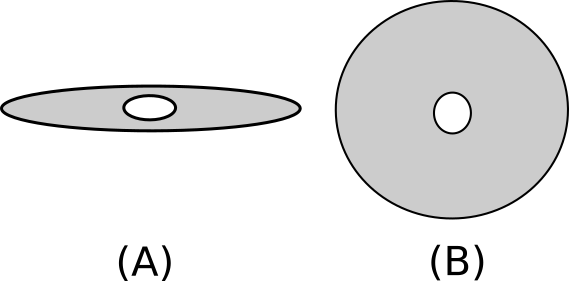
\includegraphics[width=0.50000\textwidth]{Figures/bootloader-ch/a-platter.png}
\caption{(A) Shows a platter when we see it from the side. (B) Shows a
platter when we see it from top/down.}\label{fig:a-platter}
\end{figure}

A surface of a platter is divided into a number of tracks and each track
is divided into a number of sectors. In Figure \ref{fig:tracks-sectors}
you can see how tracks and sectors are organized on a surface, the gray
circles that have the same center (cocenteric) are the tracks, a track
consists of a smaller parts which called sectors. A sector is the
smallest unit that holds data in hard disks and as you know from our
previous discussion, the first sector in a hard disk is known as boot
sector.

\begin{figure}
\centering
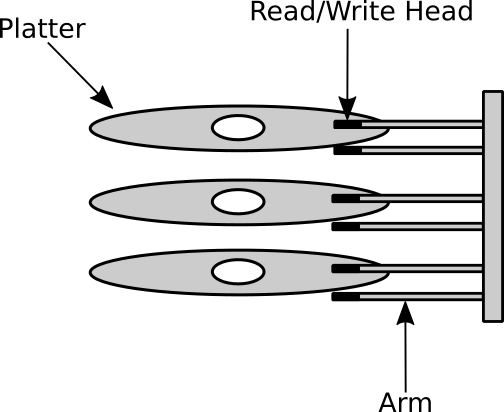
\includegraphics[width=0.50000\textwidth]{Figures/bootloader-ch/platters-arms-heads.png}
\caption{Shows how the parts of a hard disk are assembled
together.}\label{fig:platters-arms-heads}
\end{figure}

When a command is sent to the hard disk to write some data on it or read
from it, at least two mechanical moves \footnote{This fancy term
  \emph{mechanical moves} means that some physical parts of hard disk
  moves physically.} are performed. The first move is taken by the arms,
they move back or forth in order to be upon the track that contains the
data we would like to read, this operation is known as \emph{seek}
operation. So, \emph{seek time} is the time needed to put a specific
track under a read/write head. After finishing the seek operation, the
read/write head will be on the right track but, also, it will be on a
random sector \footnote{Not exactly random, can you tell why?}, to reach
the sector that we would like to read from (or write to) the platter
rotates until the read/write head becomes upon the required sector. The
speed of rotation is measured by a unit known as \emph{revolutions per
minute} (RPM) and the needed time to reach the required sector is known
as \emph{rotational latency}. Finally, the data will be
\emph{transferred} from the hard disk to the main memory, the time
needed to transfer a number of bits known as \emph{transfer time}.

Let's assume as an example a hard disk that has \lstinline!3! platters,
which means it has \lstinline!6! surfaces, arms and read/write head.
When the operating system request from the hard disk to seek a specific
track, for instance track \lstinline!3!, all \lstinline!6! heads will
seek the track \lstinline!3! and when the seek operation ends, the
\lstinline!6! heads will point to the same physical position on all
\lstinline!6! surfaces, that is, the top head of the first platter and
the bottom head of it will point to that same place, but the first one
on the top while the second is on the bottom, and so on for the other
\lstinline!4! remaining heads, the collection of all these tracks that
the heads point to at some point of time is called a \emph{cylinder}.

\begin{figure}
\centering
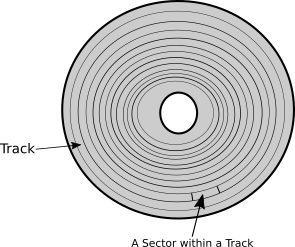
\includegraphics[width=0.50000\textwidth]{Figures/bootloader-ch/tracks-sectors.png}
\caption{Shows Tracks and Sectors on a platter's
surface.}\label{fig:tracks-sectors}
\end{figure}

Now, based on what we know about how a hard disk works, can we imagine
what happens inside the hard disk when BIOS loads a bootloader? First,
the arms will seek the track number \lstinline!0! \footnote{I didn't
  mention that previously, but yes, the bootloader resides in track
  \lstinline!0!.}, that is, the arms move back or forth until they reach
the track \lstinline!0!, then the platter rotates until the read/write
head become upon the sector \lstinline!0!, finally, the content of
sector \lstinline!0! is transferred to the main memory.

\subsection{BIOS Services}\label{bios-services}

We are in a journey of writing an operating system kernel, which means
that we are dealing with a little bit harsh environment! Do you remember
all libraries that we are lucky to have when developing normal software
(user-space software), well, none of them are available right now! And
they will not be available until we decide to make them so and work hard
to do that. Even the simple function \lstinline!printf! of C is not
available.

But that's fine, for our luck, in this environment, where there is too
little available for us to write our code, BIOS provides us with a bunch
of useful services that we can use in real mode, so, we can use these
services in our bootloader to get things done.

BIOS services are like a group of functions in high-level languages that
is provided by some library, each function does something useful and we
deal with those functions as black boxes, we don't know what's inside
these functions but we know what they do and how to use them. So,
basically, BIOS provides us a library of functions and we are going to
use some of these functions in our bootloader.

BIOS services are divided into categories, there are video services
category, disk services category, keyboard services category and so on.
Each category is identified by a unique number called \emph{interrupt
number}. In high-level world, we witnessed the same concept but with
different mechanism, for example, C standard library provides us with
many services (functions) such as input/output functions, string
manipulation functions, mathematical functions and so on, these
functions are categorized and each category is label by the
\emph{library name}, for example, all input/output functions can be
found in \lstinline!stdio.h! and so on. In BIOS, for example, the
category of video services has the interrupt number \lstinline!10h!. As
mentioned earlier, the letter\lstinline!h! after a number means that
this number represented in hexadecimal numbering system, or for short, a
hexadecimal number. Here, \lstinline!10h! doesn't equal the decimal
number \lstinline!10!. We already said that when a hexadecimal number is
mentioned we use \lstinline!h! as a postfix, also, \lstinline!0x!
\footnote{C programming language, for instance, uses this way for
  hexadecimal numbers.} can be used as a prefix instead of
\lstinline!h!, so \lstinline!10h! and \lstinline!0x10! are equivalents.

Inside each services category, there is a bunch of services, each one
can do a specific thing and they are identified by a number. Continuing
with C analogy, a service is a function labeled by a name (e.g.
\lstinline!printf!) and this function reside in a library (e.g.
\lstinline!stdio.h!) which is same as a category of services in BIOS. As
we said, the interrupt number \lstinline!10h! represents the category of
video services, and the service of printing a character on a screen
(function) is represented by the number \lstinline!0Eh!.

Interrupts is a fundamental concept in x86 architecture. What we need to
know about them right now is that they are a way to call a specific code
which is assigned to the interrupt number and calling an interrupt in
assembly is really simple, the instruction \lstinline!int! is used as
the following: \lstinline!int 10h!. That's it! We use the instruction
\lstinline!int! and gives it the interrupt number that represent the
code that we would like to call as an operand. In this example, we are
calling the code of interrupt \lstinline!10h! which is, as we mentioned
multiple time, the category of BIOS video services. When the CPU
executes this instruction, BIOS will be called and based on the
interrupt number it will know that we want to use one of available video
services, but which one exactly!

In the previous example, we actually didn't tell BIOS which video
service we would like to use and to do that we need to specify service
number in \lstinline!ah! register before calling the interrupt.

\begin{lstlisting}
mov ah, 0Eh
int 10h
\end{lstlisting}

That's it, all the BIOS services can be used in this exact way. First we
need to know what is the interrupt number that the service belongs to,
then, we need to know the number of the service itself, we put the
service number in the register \lstinline!ah! then we call the interrupt
by its number by using \lstinline!int! instruction.

The previous code calls the service of printing a character on a screen,
but is it complete yet? Actually no, we didn't specify what is the
character that we would like to print. We need something like parameters
in high-level languages to pass additional information for BIOS to be
able to do its job. Well, lucky us! the registers are here to the
rescue.

When a BIOS service needs additional information, that is, parameters.
It expects to find these information in a specific register. For
example, the service \lstinline!0Eh! in interrupt \lstinline!10h!
expects to find the character that the user wants to print in the
register \lstinline!al!, so, the register \lstinline!al! is one of
service \lstinline!0Eh! parameters. The following code requests from
BIOS to print the character \lstinline!S! on the screen:

\begin{lstlisting}
mov ah, 0Eh
mov al, 'S'
int 10h
\end{lstlisting}

\subsection{A Little Bit More of x86 Assembly and
NASM}\label{a-little-bit-more-of-x86-assembly-and-nasm}

We need to learn a couple more things about x86 assembly to be able to
start. In NASM, each line in the source code has the following format.

\begin{lstlisting}
label: instruction operands
\end{lstlisting}

The label is optional, the operands depend on x86 instruction in use, if
it doesn't get any operand then we don't need to write them. To write
comments on NASM we begin with semi-colon and write whatever we like
after it as a comment and the rest of the source line will be considered
as a part of the comment.

A label is a way to give an instruction or a group of instructions a
meaningful name, then we can use this name in other places in the source
code to refer to this instruction/group of instructions, we can use
labels for example to call this group of instructions or to get the
starting memory address of these instructions. Sometimes, we may use
labels to make the code more readable.

We can say that a label is something like the name of a function or
variable in C, as we know a variable name in C is a meaningful name that
represents the memory address of a location in the main memory that
contains the value of a variable, the same holds true for a function
name. Labels in NASM works in the same way, under the hood it represents
a memory address. The colon in label is also optional.

\begin{lstlisting}
print_character_S_with_BIOS:
    mov ah, 0Eh
    mov al, 'S'
    int 10h
\end{lstlisting}

You can see in the code above, we gave a meaningful name for the bunch
of instructions that prints the character \lstinline!S! on the screen.
After defining this label in our source code, we can use it anywhere in
the same source code to refer to this bunch of instructions.

\begin{lstlisting}
call_video_service int 10h
\end{lstlisting}

This is another example of labels. This time we eliminated the optional
colon in label's name and the label here points to only one instruction.
Please note that extra whitespaces and new lines doesn't matter in NASM,
so, the following is equivalent to the one above.

\begin{lstlisting}
call_video_service
    int 10h
\end{lstlisting}

Consider the following code, what do you think it does?

\begin{lstlisting}
print_character_S_with_BIOS:
    mov ah, 0Eh
    mov al, 'S'

call_video_service:
    int 10h
\end{lstlisting}

Still it prints \lstinline!S! on the screen. Introducing labels in the
source code doesn't change its flow, the code will be executed
sequentially whether we used the labels or not. The sequence of
execution will not be changed by merely using labels, if we need to
change the sequence of execution we need to use other methods than
labels. You already know one of these methods which is calling an
interrupt. So, we can say that labels are more general than a variable
name or function name in C. A label is a human-readable name for a
memory location which can contain anything, code or data!

\subsubsection{Jump and Return
Unconditionally}\label{jump-and-return-unconditionally}

Let's start this section with a simple question. What happens when we
call a function in C? Consider the following C code.

\begin{lstlisting}[language=C]
main()
{
    int result = sum( 5, 3 );

    printf( "%d\n", result );
}
\end{lstlisting}

Here, the function \lstinline!main! called a function named
\lstinline!sum!, this function reside in a different region in memory
and by calling it we are telling the processor to go to this different
region of memory and execute what's inside it, the function
\lstinline!sum! is going to do its job, and after that, in some magical
way, the processor is going to return to the original memory region
where we called \lstinline!sum! from and proceed the execution of the
code that follows the calling of \lstinline!sum!, in this case, the
\lstinline!printf! function. How does the processor know where to return
after completing the execution of \lstinline!sum!?

The function which call another is named \emph{caller} while the
function which is called by the caller named \emph{callee}, in the above
C code, the caller is the function \lstinline!main! while the callee is
the function \lstinline!sum!.

\paragraph{A Glance on a Computer
Architecture}\label{a-glance-on-a-computer-architecture}

When a program is running, a copy of its machine code is loaded in the
main memory, this machine code is a sequence of instructions which are
understandable by the processor, these instructions are executed by the
processor sequentially, that is, one after another in each cycle in the
processor, also, the data that the code being executed is dealing with
is stored in the same main memory. This architecture where both code and
data are stored in the same memory and the processor uses this memory to
read the instructions that should be executed, and manipulate the data
which is stored in the same memory is known as \emph{von Neumann
architecture}. There is another well-known architecture called
\emph{Harvard architecture} where the code and data are stored in two
different memories, x86 uses \emph{von Neumann architecture}.

When a processor starts a new \emph{instruction cycle}, it fetches the
next instruction that should be executed from the main memory and
executes it \footnote{The instruction cycle is also called
  \emph{fetch-decode-execute cycle}.}. Each \emph{memory location} in
the main memory is represented and referred to by a unique \emph{memory
address}, that means each instruction in the machine code of a loaded
program has a unique memory address, consider the following hypothetical
example of the memory addresses of each instruction in the previous C
code, note that the memory addresses in this example are by no means
accurate.

\begin{lstlisting}[language=C]
100 main() {
110    int result = sum( 5, 3 );
120    printf( "%d\n", result );
130 }

250 int sum( int firstNumber, int secondNumber ) {
260     return firstNumber + secondNumber;
270 }
\end{lstlisting}

The number on the left is the hypothetical memory address of the code
line in the right, that means the function \lstinline!main! starts from
the memory address \lstinline!100! and so on. Also, we can see that the
callee \lstinline!sum! resides in a far region of memory from the caller
\lstinline!main!.

\emph{Program Counter} is a part of computer architecture which stores
the \emph{memory address} for the instruction that will be executed in
the next instruction cycle of the processor. In x86, the program counter
is a register known as \emph{instruction pointer} and its name is
\lstinline!IP! in 16-bit and \lstinline!EIP! in 32-bit.

When the above C code runs for the first time, the value of the
instruction pointer will be \lstinline!100!, that is, the memory address
of the starting point of \lstinline!main! function. When the instruction
cycle starts, it reads the value of the instruction pointer register
\lstinline!IP!/\lstinline!EIP! which is \lstinline!100!, it fetches the
instruction which is stored in the memory location \lstinline!100! and
executes it \footnote{For the simplicity of explanation, the details of
  \emph{decoding} have been eliminated.}, then the memory address of the
next instruction \lstinline!110! will be stored in the instruction
pointer register for the next instruction cycle. When the processor
finishes the execution of the instruction of the memory location
\lstinline!110!, this time, the value of \lstinline!IP!/\lstinline!EIP!
will be \lstinline!250! instead of \lstinline!120! because, you know, we
are calling the function \lstinline!sum! which resides in the memory
location \lstinline!250!.

Each running program has a \emph{stack} which is a region of the
program's memory \footnote{The stack as a region of memory (x86 stack)
  is not same as the \emph{data structure} stack, the former implements
  the latter.}, that is, a place in the memory that belongs to the
program and can store data, we will examine the details of stack later,
but what is important for us now is the following, when another function
is called, in our case \lstinline!sum!, the memory address of the next
instruction of the callee \lstinline!main! is \emph{pushed} \footnote{Push
  means store something in a stack, this term is applicable for both x86
  stack and the data structure stack, as we have said previously, x86
  stack is an implementation of the stack data structure.} into the
stack, so the memory address \lstinline!120! will be pushed into the
stack before calling \lstinline!sum!, this address is called
\emph{return address}. Now, assume that the processor is executing the
instruction in the memory location \lstinline!270!, that is, finishing
the execution of the callee \lstinline!sum!, after that the processor
will find the return address which is \lstinline!120! in the stack, get
it and put it in the register \lstinline!IP!/\lstinline!EIP! for the
next instruction cycle \footnote{By the way, this is, partially, the
  cause of buffer overflow bugs.}. So, this is the answer of our
original question in the previous section ``How does the processor know
where to return after completing the execution of \lstinline!sum!?''.

\paragraph{\texorpdfstring{The Instructions \texttt{call} and
\texttt{ret}}{The Instructions call and ret}}\label{the-instructions-call-and-ret}

The instruction \lstinline!call! in assembly works exactly in the same
way that we have explained in the previous section, it is used to call a
code that resides in a given memory address. The instruction
\lstinline!call! pushes the return address into the stack and to return
to the caller, the callee should use the instruction \lstinline!ret!
when it finishes. The instruction \lstinline!ret! gets the return
address from the stack \footnote{Actually it \emph{pop}s the value since
  we are talking about stack here.} and use it to resume the execution
of the caller. Consider the following example.

\begin{lstlisting}
print_two_times:
    call print_character_S_with_BIOS
    call print_character_S_with_BIOS
    ret

print_character_S_with_BIOS:
    mov ah, 0Eh
    mov al, 'S'
    int 10h
    ret
\end{lstlisting}

You can see here that we have used the code sample
print\_character\_S\_with\_BIOS to define something like C functions by
using the instructions \lstinline!call! and \lstinline!ret!. It should
be obvious that the code of \lstinline!print_two_times! prints the
character \lstinline!S! two times, as we have said previously, a label
represents a memory address and print\_character\_S\_with\_BIOS is a
label, the operand of \lstinline!call! is the memory address of the code
that we wish to call, the instructions of
print\_character\_S\_with\_BIOS will be executed sequentially until the
processor reaches the instruction \lstinline!ret!, at this point, the
return address is obtained from the stack and the execution of the
caller is resumed.

\lstinline!call! performs an \emph{unconditional jump}, that means the
processor reaches to a \lstinline!call! instruction, it will always call
the callee, without any condition, later in this chapter we will see an
instruction that performs a \emph{conditional jump}, which only calls
the callee when some condition is satisfied, otherwise, the execution of
the caller continues sequentially with no flow change.

\subsubsection{The One-Way Unconditional
Jump}\label{the-one-way-unconditional-jump}

Like \lstinline!call!, the instruction \lstinline!jmp! jumps to the
specified memory address, but unlike \lstinline!call!, it doesn't store
the return address in the stack which means \lstinline!ret! cannot be
used in the callee to resume the caller's execution. We use
\lstinline!jmp! when we want to jump to a code that we don't need to
return from, \lstinline!jmp! has the same functionality of
\lstinline!goto! statement in C. Consider the following example.

\begin{lstlisting}
print_character_S_with_BIOS:
    mov ah, 0Eh
    mov al, 'S'
    jmp call_video_service

print_character_A_with_BIOS:
    mov ah, 0Eh
    mov al, 'A'

call_video_service:
    int 10h
\end{lstlisting}

Can you guess what is the output of this code? it is \lstinline!S! and
the code of the label \lstinline!print_character_A_with_BIOS! will never
be executed because of the line \lstinline!jmp call_video_service!. If
we remove the line of \lstinline!jmp! from this code sample,
\lstinline!A! will be printed on the screen instead of \lstinline!S!.
Another example which causes infinite loop.

\begin{lstlisting}
infinite_loop:
    jmp infinite_loop
\end{lstlisting}

\subsubsection{Comparison and Conditional
Jump}\label{comparison-and-conditional-jump}

In x86 there is a special register called \emph{FLAGS} register
\footnote{In 32-bit x86 processors its name is \emph{EFLAGS} and in
  64-bit its name is \emph{RFLAGS}.}. It is the \emph{status register}
which holds the current status of the processor. Each usable bit of this
register has its own purpose and name, for example, the first bit (bit
\lstinline!0!) of FLAGS register is known as \emph{Carry Flag}
(\lstinline!CF!) and the seventh bit (bit \lstinline!6!) is known as
\emph{Zero Flag} (\lstinline!ZF!).

Many x86 instructions use \lstinline!FLAGS! register to store their
result on, one of those instructions is \lstinline!cmp! which can be
used to compare two integers which are passed to it as operands, when a
comparison finishes, the processor stores the its result in
\lstinline!FLAGS! register. The following line compares the value which
reside in the register \lstinline!al! with \lstinline!5!:
\lstinline!cmp al, 5!.

Now, let's say that we would like to jump to a piece of code only if the
value of \lstinline!al! equals \lstinline!5!, otherwise, the code of the
caller continues without jumping. There are multiple instructions that
perform \emph{conditional} jump based on the result of \lstinline!cmp!.
One of these instructions is \lstinline!je! which means \emph{jump if
equal}, that is, if the two operands of the \lstinline!cmp! instruction
equals each other, then jump to the specified code. Another conditional
jump instruction is \lstinline!jne! which means \emph{jump if not
equal}, there are other conditional jump instructions to handle the
other cases. We can see that the conditional jump instructions have the
same functionality of \lstinline!if! statement in C. Consider the
following example.

\begin{lstlisting}
main:
    cmp al, 5
    je the_value_equals_5
    ; The rest of the code of `main` label
\end{lstlisting}

This example jumps to the code of the label
\lstinline!the_value_equals_5! if the value of the register
\lstinline!al! equals \lstinline!5!. In C, the above assembly example
will be something like the following.

\begin{lstlisting}[language=C]
main() 
{
    if ( register_al == 5 )
        the_value_equals_5();

    // The rest of the code
}
\end{lstlisting}

Like \lstinline!jmp!, but unlike \lstinline!call!, conditional jump
instructions don't push the return address into the stack, which means
the callee can't use \lstinline!ret! to return and resume caller's code,
that is, the jump will be \emph{one way jump}. We can also imitate
\lstinline!while! loop by using conditional jump instructions and
\lstinline!cmp!, the following example prints \lstinline!S! five times
by looping over the same bunch of code.

\begin{lstlisting}
mov bx, 5

loop_start:
    cmp bx, 0
    je loop_end
    
    call print_character_S_with_BIOS
    
    dec bx
    
    jmp loop_start
    
loop_end:
    ; The code after loop
\end{lstlisting}

You should be familiar with the most of the code of this sample, first
we assign the value \lstinline!5! to the register \lstinline!bx!
\footnote{Can you tell why we used \lstinline!bx! instead of
  \lstinline!ax!? {[}Hint: review the code of
  print\_character\_S\_with\_BIOS.{]}}, then we start the label
\lstinline!loop_start! which the first thing it does is comparing the
value of \lstinline!bx! with \lstinline!0!, when \lstinline!bx! equals
\lstinline!0! the code jumps to the label \lstinline!loop_end! which
contains the code after the loop, that is, it means that the loop ended.
When \lstinline!bx! doesn't equal \lstinline!0! the label
print\_character\_S\_with\_BIOS will be called to print \lstinline!S!
and return to the caller \lstinline!loop_start!, after that the
instruction \lstinline!dec! is used to decrease \lstinline!1! form its
operand, that is \lstinline!bx = bx - 1!, finally, the label
\lstinline!loop_start! will be called again and the code repeats until
the value of \lstinline!bx! reaches to \lstinline!0!. The equivalent
code in C is the following.

\begin{lstlisting}[language=C]
int bx = 5;

while ( bx != 0 )
{
    print_character_S_with_BIOS();
    bx--;
}

// The code after loop
\end{lstlisting}

\subsubsection{Load String}\label{load-string}

It is well-known that \lstinline!1! byte equals \lstinline!8! bits.
Moreover, there are two size units in x86 other than a byte. The first
one is known as a \emph{word} which is \lstinline!16! bits, that is,
\lstinline!2! bytes, and the second one is known as \emph{doubleword}
which is \lstinline!32! bits, that is, \lstinline!4! bytes. Some x86
instructions have multiple variants to deal with these different size
units, while the functionality of an instruction is the same, the
difference will be in the size of the data that a variant of instruction
deals with. For example, the instruction \lstinline!lods! has three
variants \lstinline!lodsb! which works a \textbf{b}yte,
\lstinline!lodsw! which works with a \textbf{w}ord and
\lstinline!loadsd! which works with a \textbf{d}oubleword.

To simplify the explanation, let's consider \lstinline!lodsb! which
works with a single byte, its functionality is too simple, it reads the
value of the register \lstinline!si! which is interpreted as a memory
address by the instruction, then it transfers a byte from the content of
that memory address to the register \lstinline!al!, finally, it
increments the value of \lstinline!si! by \lstinline!1! byte. The same
holds true for the other variants of \lstinline!lods!, only the size of
the data, the used registers and the increment size are different, the
register which is used by \lstinline!lodsw! is \lstinline!ax! \footnote{Because
  the size of \lstinline!ax! is a \textbf{word}} and \lstinline!si! is
incremented by \lstinline!2! bytes, while \lstinline!lodsd! uses the
register \lstinline!eax! \footnote{Because the size of \lstinline!eax!
  is a \textbf{doubleword}.} and \lstinline!si! is incremented by
\lstinline!4! bytes. \footnote{As an exercise, try to figure out why are
  we explaining the instruction \lstinline!lodsb! in this chapter, what
  is the relation between this instruction and the bootloader that we
  are going to write? Hint: Review the code of
  print\_character\_S\_with\_BIOS and how to print a character by using
  BIOS services. If you can't figure the answer out don't worry, you
  will get it soon.}

\subsubsection{NASM's
Pseudoinstructions}\label{nasms-pseudoinstructions}

When you encounter the prefix \footnote{In linguistics, which is the
  science that studies languages, a prefix is a word (actually a
  morpheme) that is attached in the beginning of another word and
  changes its meaning, for example, in \textbf{un}do, \textbf{un} is a
  prefix.} \emph{pseudo} before a word, you should know that it
describes something fake, false or not real \footnote{For example, in
  algorithm design which is a branch of computer science, the term
  \textbf{pseudo}code means a code that is written in a fake programming
  language. Another example is the word \textbf{pseudo}science: A
  statement is a pseudoscience when it is claimed to be a scientific
  fact, but in reality it is not, that is, it doesn't follow the
  scientific method.}. NASM provides us with a number of
\textbf{pseudo}instructions, that is, they are not real x86
instructions, the processor doesn't understand them and they can't be
used in other assemblers \footnote{Unless, of course, they are provided
  in the other assembler as pseudoinstructions.}, on the other hand,
NASM understands those instructions and can translate them to something
understandable by the processor. They are useful, and we are going to
use them to make the writing of the bootloader easier.

\paragraph{Declaring Initialized Data}\label{declaring-initialized-data}

The concept of \emph{declaring something} is well-known by the
programmers, In C for example, when you \emph{declare} a function, you
are announcing that this function \emph{exists}, it is there, it has a
specific name and takes the declared number of parameters \footnote{It
  is important to note that \emph{declaring} a function in C differs
  from \emph{defining} a function, the following declares a function:
  \lstinline!int foo();! You can see that the code block (the
  implementation) of \lstinline!foo! is not a part of the declaration,
  once the code block of the function is presented, we say this is the
  \emph{definition} of the function.}. The same concept holds true when
you declare a variable, you are letting the rest of the code know that
there exists a variable with a specific name and type. When we declare a
variable, without assigning any value to it, we say that this variable
is \emph{uninitialized}, that is, no initial value has been assigned to
this variable when it was declared, later on, a value will be assigned
to the variable, but not as early of its declaration. In contrast, a
variable is \emph{initialized} when a value is assigned to it when it's
declared.

The pseudoinstructions \lstinline!db!, \lstinline!dw!, \lstinline!dd!,
\lstinline!dq!, \lstinline!dt!, \lstinline!ddq! and \lstinline!do! help
us to initialize a memory location with some data, and with using labels
when can mimic the concept of initialized variables in C. As an example,
let's consider \lstinline!db! which declares and initializes a byte of
data, the second letter of \lstinline!db! means \emph{b}ytes.

\begin{lstlisting}
db 'a'
\end{lstlisting}

The above example reserves a byte in the memory, this is the declaration
step, then the character \lstinline!a! will be stored on this reserved
byte of the memory, which is the initialization step.

\begin{lstlisting}
db 'a', 'b', 'c'
\end{lstlisting}

In the above example we have used comma to declare three bytes and store
the values \lstinline!a!, \lstinline!b! and \lstinline!c! respectively
on them, also, on memory these values will be stored
\emph{contiguously}, that is, one after another, the memory location
(hence, the memory address) of the value \lstinline!b! will be right
after the memory location of value \lstinline!a! and the same rule
applies for \lstinline!c!. Since \lstinline!a!, \lstinline!b! and
\lstinline!c! are of the same type, a character, we can write the
previous code as the following and it gives as the same result.

\begin{lstlisting}
db 'abc'
\end{lstlisting}

Also, we can declare different types of data in the same source line,
given the above code, let's say that we would like to store the number
\lstinline!0! after the character \lstinline!c!, this can be achieved by
simply using a comma.

\begin{lstlisting}
db 'abc', 0
\end{lstlisting}

Now, to make this data accessible from other parts of the code, we can
use a label to represent the starting memory address of this data.
Consider the following example, it defines the label
\lstinline!our_variable!, after that, we can use this label to refer to
the initialized data.

\begin{lstlisting}
our_variable db 'abc', 0
\end{lstlisting}

\paragraph{\texorpdfstring{Repeating with
\texttt{times}}{Repeating with times}}\label{repeating-with-times}

To repeat some source line multiple times, we can use the
pseudoinstruction \lstinline!times! which takes the number of
repetitions as first operand and the instruction that we would like to
execute repeatedly as second operand. The following example prints
\lstinline!S! five times on the screen.

\begin{lstlisting}
times 5 call print_character_S_with_BIOS
\end{lstlisting}

Not only normal x86 instructions can be used with \lstinline!times! as
second operand, also NASM's pseudoinstructions can be used with
\lstinline!times!. The following example reserves \lstinline!100! bytes
of the memory and fills them with \lstinline!0!.

\begin{lstlisting}
times 100 db 0
\end{lstlisting}

\subsubsection{NASM's Special
Expressions}\label{nasms-special-expressions}

In programming languages, an \emph{expression} is a part in the code
that evaluates a value, for example, \lstinline!x + 1! is an expression,
also, \lstinline!x == 5! is an expression. On the other hand, a
\emph{statement} is a part of the code that performs some action, for
example, in C, \lstinline!x = 15 * y;! is a statement that assigns the
values of an expression to the variable \lstinline!x!.

NASM has two special expressions, the first one is \lstinline!$! which
points to the beginning of the \emph{assembly position} of the current
source line. So, one way of implementing infinite loop is the following:
\lstinline!jmp $!. The second special expression is \lstinline!$$! which
points to the beginning of the current \emph{section} of assembly code.

\subsection{The Bootloader}\label{the-bootloader}

As you have learned previously, the size of the bootloader should be
\lstinline!512! bytes, the firmware loads the bootloader in the memory
address \lstinline!07C0h!, also, the firmware can only recognize the
data in the first sector as a bootloader when that data finishes with
the magic code \lstinline!AA55h!. When 539kernel's bootloader starts, it
shows two messages for the user, the first one is
\lstinline!The Bootloader of 539kernel.! and the second one
\lstinline!The kernel is loading...!, after that, it is going to read
the disk to find 539kernel and load it to memory, after loading
539kernel to memory, the bootloader gives the control to the kernel by
jumping to the start code of the kernel.

Right now, 539kernel doesn't exist \footnote{Actually it does! But you
  know what I mean.}, we haven't write it yet, so, in our current stage,
instead of loading 539kernel, the bootloader is going to load a code
that prints \lstinline"Hello World!, From Simple Assembly 539kernel!".
In this section, we are going to write two assembly files, the
bootloader \lstinline!bootstrap.asm! and \lstinline!simple_kernel.asm!
which is the temporary replacement of 539kernel, also,
\lstinline!Makefile! which compiles the source code of the assembly
files will be presented in this section.

\subsubsection{Implementing the
Bootloader}\label{implementing-the-bootloader}

Till now, you have learned enough to understand the most of the
bootloader that we are going to implement, however, some details have
not been explained in this chapter and have been delayed to be explained
later. The first couple lines of the bootloader is an example of
concepts that have not been explained, our bootloader source code starts
with the following.

\begin{lstlisting}
start:
    mov ax, 07C0h
    mov ds, ax
\end{lstlisting}

First, we define a label named \lstinline!start!, there is no practical
reason to define this label (such as jump to it for example), the only
reason of defining it, is the readability of the code, when someone else
tries to read the code, it should be obvious for her that
\lstinline!start! is the starting point of executing the bootloader.

The job of next two lines is obvious, we are moving the hexadecimal
number \lstinline!07C0! to the register \lstinline!ax! then we move the
same value to the register \lstinline!ds! through \lstinline!ax!, note
that we can't store the value \lstinline!07C0! directly in
\lstinline!ds! by using \lstinline!mov! as the following:
\lstinline!mov ds, 07C0h!, due to that, we have put the value on
\lstinline!ax! and then moved it to \lstinline!ds!, so, our goal was to
set the value \lstinline!07C0! in the register \lstinline!ds!, this
restriction of not being able to store to \lstinline!ds! directly is
something that the processor architecture decides. Now, you may ask why
we want the value \lstinline!07C0! in the register \lstinline!ds!, this
is a story for another chapter, just take these two lines on faith, and
you will learn later the purpose of them. Let's continue.

\begin{lstlisting}
    mov si, title_string
    call print_string
    
    mov si, message_string
    call print_string
\end{lstlisting}

This block of code prints the two messages that we mentioned earlier,
both of them are represented by a separate label
\lstinline!title_string! and \lstinline!message_string!, you can see
that we are calling the code of a label \lstinline!print_string! that we
didn't define yet, its name indicates that it prints a \emph{string} of
characters, and you can infer that the function \lstinline!print_string!
receives the memory address of the string that we would like to print as
a parameter in the register \lstinline!si!, the implementation of
\lstinline!print_string! will be examined in a minute.

\begin{lstlisting}
    call load_kernel_from_disk
    jmp 0900h:0000
\end{lstlisting}

These two lines represent the most important part of any bootloader,
first a function named \lstinline!load_kernel_from_disk! is called, we
are going to define this function in a moment, as you can see from its
name, it is going to load the code of the kernel from disk into the main
memory and this is the first step that makes the kernel able to take the
control over the system. When this function finishes its job and
returns, a jump is performed to the memory address
\lstinline!0900h:000!, but before discussing the purpose of the second
line let's define the function \lstinline!load_kernel_from_disk!.

\begin{lstlisting}
load_kernel_from_disk:
    mov ax, 0900h
    mov es, ax
\end{lstlisting}

This couple of lines, also, should be taken on faith. You can see, we
are setting the value \lstinline!0900h! on the register \lstinline!es!.
Let's move to the most important part of this function.

\begin{lstlisting}
    mov ah, 02h
    mov al, 01h
    mov ch, 0h
    mov cl, 02h
    mov dh, 0h
    mov dl, 80h
    mov bx, 0h
    int 13h
    
    jc kernel_load_error

    ret
\end{lstlisting}

This block of code \textbf{loads} the kernel from the disk into the
memory and to do that it uses the BIOS Service \lstinline!13h! which
provides services that are related to hard disks. The service number
which is \lstinline!02h! is specified on the register \lstinline!ah!,
this service reads sectors from the hard disk and loads them into the
memory. The value of the register \lstinline!al! is the number of
sectors that we would like to read, in our case, because the size of our
temporary kernel \lstinline!simple_kernel.asm! doesn't exceed
\lstinline!512! bytes we read only \lstinline!1! sector. Before
discussing the rest of passed values to the BIOS service, we need to
mentioned that our kernel will be stored right after the bootloader on
the hard disk, and based on this fact we can set the correct values for
the rest registers which represent the disk location of the content that
we would like to load.

The value of register \lstinline!ch! is the number of the track that we
would like to read from, in our case, it is the track \lstinline!0!. The
value of the register \lstinline!cl! is the sector number that we would
like to read its content, in our case, it is the second sector. The
value of the register \lstinline!dh! is the head number. The value of
\lstinline!dl! specifies which the type of disk that we would like to
read from, the value \lstinline!0h! in this register means that we would
like to read the sector from a floppy disk, while the value
\lstinline!80h! means we would like to read from the hard disk
\lstinline!#0! and \lstinline!81h! for hard disk \lstinline!#1!, in our
case, the kernel is stored in the hard disk \lstinline!#0!, so, the
value of \lstinline!dl! should be \lstinline!80h!. Finally, the value of
the register \lstinline!bx! is the memory address that the content will
be loaded into, in our case, we are reading one sector, and its content
will be stored on the memory address \lstinline!0h! \footnote{Not
  exactly the memory address \lstinline!0h!, in fact, it will be loaded
  in offset \lstinline!0! inside a segment that starts at
  \lstinline!0900h!. Don't worry, these details will be examined later
  in the next chapter \ref{ch-x86}.}.

When the content is loaded successfully, the BIOS Service
\lstinline!13h:02h! is going to set the carry flag \footnote{Which is
  part of FLAGS register as we mentioned earlier} to \lstinline!0!,
otherwise, it sets the carry flag to \lstinline!1! and stores the error
code in register \lstinline!ax!, the instruction \lstinline!jc! is a
conditional jump instruction that jumps when \lstinline!CF = 1!, that
is, when the value of the carry flag is \lstinline!1!. That means our
bootloader is going to jump to the label \lstinline!kernel_load_error!
when the kernel isn't loaded correctly.

If the kernel is loaded correctly, the function
\lstinline!load_kernel_from_disk! returns by using the instruction
\lstinline!ret! which makes the processor to resume the main code of our
bootloader and executes that instruction which is after
\lstinline!call load_kernel_from_disk!, this next instruction is
\lstinline!jmp 0900h:0000! which gives the control to the kernel by
jumping to its starting point, that is, the memory location where we
loaded our kernel in. In this time, the operand of \lstinline!jmp! is an
\textbf{explicit} memory address \lstinline!0900h:0000!, it has two
parts, the first part is the one before the colon, you can see that it
is the same value that we have loaded in the register \lstinline!es! in
the beginning of \lstinline!load_kernel_from_disk! function. The second
part of the memory address is the one after the colon, it is
\lstinline!0h! \footnote{Here, \lstinline!0h! is equivalent to
  \lstinline!0000!.} which is the \emph{offset} that we have specified
in the register \lstinline!bx! in \lstinline!load_kernel_from_disk!
before calling \lstinline!02h:13h!, the both parts combined represent
the memory address that we have loaded our kernel into and the details
of the two parts of this memory address will be discussed in chapter
\ref{ch-x86}.

Now we have finished the basic code of the bootloader, we can start
defining that labels that we have used before in its code. We start with
the label \lstinline!kernel_load_error! which simply prints an error
message, the function \lstinline!print_string! is used to perform that,
after printing the message, nothing can be done, so,
\lstinline!kernel_load_error! enters an infinite loop.

\begin{lstlisting}
kernel_load_error:
    mov si, load_error_string
    call print_string
    
    jmp $
\end{lstlisting}

Our previous samples of using the BIOS Service \lstinline!0Eh:10h! were
printing only one character, in real world, we need to print a
\textbf{string} of characters and that's what the function
\lstinline!print_string! exactly does, it takes the memory address which
is stored in the register \lstinline!si! and prints the character which
is stored in this memory location, then it moves to the next memory
address and prints the character which is stored in this next memory
location and so on, that is, \lstinline!print_string! prints a string
character by character. So, you may ask, how \lstinline!print_string!
can know when should it stop?

A string in C programming language, as in our situation, is an array of
characters, and the same problem of ``where does a string end'' is
encountered in C programming language, to solve the problem, each string
in C programming language ends with a special character named \emph{null
character} and represented by the symbol \lstinline!\0! in C \footnote{This
  type of strings named \emph{null-terminated strings}.}, so, you can
handle any string in C character by character and once you encounter the
null character \lstinline!\0! that means you have reached the end of
that string. We are going to use the same mechanism in our
\lstinline!print_string! function to recognize the end of a string by
putting the value \lstinline!0! as a marker at the end of the it. By
using this way, we can now use the service \lstinline!0Eh:10h! to print
any string, character by character, through a loop and once we encounter
the value \lstinline!0! we can stop the printing.

\begin{lstlisting}
print_string:
    mov ah, 0Eh

print_char:
    lodsb
    
    cmp al, 0
    je printing_finished
    
    int 10h
    
    jmp print_char

printing_finished:
    mov al, 10d ; Print new line
    int 10h
    
    ; Reading current cursor position
    mov ah, 03h
    mov bh, 0
    int 10h
    
    ; Move the cursor to the beginning
    mov ah, 02h
    mov dl, 0
    int 10h

    ret
\end{lstlisting}

When \lstinline!print_string! starts, the BIOS service number
\lstinline!0Eh! is loaded in \lstinline!ah!, this operation needs to
execute just one time for each call of \lstinline!print_string!, so it
is not a part of the next label \lstinline!print_char! which is also a
part of \lstinline!print_string! and it will be executed right after
moving \lstinline!0Eh! to \lstinline!ah!.

As you can remember, that parameter of \lstinline!print_string! is the
memory address which contains the beginning of the string that we would
like to print, this parameter is passed to \lstinline!print_string! via
the register \lstinline!si!, so, the first thing \lstinline!print_char!
does is using the instruction \lstinline!lodsb! which is going to
transfer the first character of the string to the register
\lstinline!al! and increase the value of \lstinline!si! by \lstinline!1!
byte, after that, we check the character that has been transferred from
the memory to \lstinline!al!, if it is \lstinline!0!, that means we have
reached to the end of the string and the code jumps to the label
\lstinline!printing_finished!, otherwise, the interrupt \lstinline!10h!
of BIOS is called to print the content of the register \lstinline!al! on
the screen, then we jump to \lstinline!print_char! again to repeat this
operation until we reach the end of the string.

When printing a string finishes, the label \lstinline!printing_finished!
starts by printing a new line after the string, the new line is
represented by the number \lstinline!10! in ASCII, after that we are
going to use the service \lstinline!03h! to read the current position of
the cursor, then we use the service \lstinline!02h! to set the cursor to
position \lstinline!0! by passing it to the register \lstinline!dl!,
otherwise, the messages in the new lines will be printed in the position
where the previous string finished, finally the function returns to the
caller by using the instruction \lstinline!ret!.

\begin{lstlisting}
title_string        db  'The Bootloader of 539kernel.', 0
message_string      db  'The kernel is loading...', 0
load_error_string   db  'The kernel cannot be loaded', 0
\end{lstlisting}

The code above defines the strings that have been used previously in the
source code, note the last part of each string, which is the null
character that indicates the end of a string \footnote{Exercise: What
  will be the behavior of the bootloader if we remove the null character
  from \lstinline!title_string! and \lstinline!message_string! and keep
  it in \lstinline!load_error_string!?}.

Now, we have written our bootloader and the last thing to do is to put
the \emph{magic code} in the end of it, the magic code which is a
\lstinline!2! bytes value should reside in the last two bytes in the
first sector, that is, in the locations \lstinline!510! and
\lstinline!511! (the location number starts from \lstinline!0!),
otherwise, the firmware will not recognize the content of the sector as
a bootloader. To ensure that the magic code is written on the correct
location, we are going to fill with zeros the empty space between the
last part of bootloader code and the magic code, this can be achieved by
the following line.

\begin{lstlisting}
times 510-($-$$) db 0
\end{lstlisting}

So, the instruction \lstinline!db! will be called \lstinline!510-($-$$)!
times, this expression gives us the remaining empty space in our
bootloader before the magic code, and because the magic code is a
\lstinline!2! bytes value, we subtract \lstinline!($-$$)! from
\lstinline!510! instead of \lstinline!512!, we will use these two bytes
for the magic code, the expression \lstinline!($-$$)! uses the special
expressions of NASM \lstinline!$! and \lstinline!$$! and it gives the
size of the bootloader code until the current line. Finally, the magic
code is presented.

\begin{lstlisting}
dw 0xAA55
\end{lstlisting}

\subsubsection{\texorpdfstring{Implementing
\texttt{simple\_kernel.asm}}{Implementing simple\_kernel.asm}}\label{implementing-simple_kernel.asm}

The \lstinline!simple_kernel.asm! which the bootloader loads is too
simple, it prints the message
\lstinline"Hello World!, From Simple Assembly 539kernel!", we don't need
to go through its code in details since you know most of it.

\begin{lstlisting}
start:
    mov ax, cs
    mov ds, ax

    ; --- ;
    
    mov si, hello_string
    call print_string
    
    jmp $

print_string:
    mov ah, 0Eh

print_char:
    lodsb
    
    cmp al, 0
    je done
    
    int 10h
    
    jmp print_char

done:
    ret
    
hello_string db 'Hello World!, From Simple Assembly 539kernel!', 0
\end{lstlisting}

The only lines that you are not familiar with until now are the first
two lines in the label \lstinline!start! which will be explained in
details in chapter \ref{ch-x86}. Finally the \lstinline!Makefile! is the
following.

\begin{lstlisting}[language=make]
ASM = nasm
BOOTSTRAP_FILE = bootstrap.asm 
KERNEL_FILE = simple_kernel.asm

build: $(BOOTSTRAP_FILE) $(KERNEL_FILE)
    $(ASM) -f bin $(BOOTSTRAP_FILE) -o bootstrap.o
    $(ASM) -f bin $(KERNEL_FILE) -o kernel.o
    dd if=bootstrap.o of=kernel.img
    dd seek=1 conv=sync if=kernel.o of=kernel.img bs=512
    qemu-system-x86_64 -s kernel.img

clean:
    rm -f *.o
\end{lstlisting}


	
	\newpage
    \thispagestyle{plain}
    \mbox{}
    
    \chapter{Chapter 2: An Overview of x86 Architecture}\label{ch-x86}

\section{Introduction}\label{introduction}

In our situation, and by using modern terminology, we can view the
processor as a \emph{library} and \emph{framework}. A library because it
provides us with a bunch of instructions to perform whatever we want,
and a framework because it has general rules that organize the overall
environment of execution, that is, it forces us to work in a specific
way. We have seen some aspects of the first part when we have written
the bootloader, that is, we have seen the processor as a library. In
this chapter, we are going to see how the processor works as a framework
by examining some important and basic concepts of x86. We need to
understand these concepts to start the real work of writing 539kernel.

\section{x86 Operating Modes}\label{x86-operating-modes}

In x86 an operating mode specifies the overall picture of the processor,
such as the maximum size of available registers, the available advanced
features for the running operating system, the restrictions and so on.

When we developed the bootloader in the previous chapter we have worked
with an x86 operating mode named \emph{real address mode} (or for short
\emph{real mode}) which is an old operating mode that is still supported
by modern x86 processors for the sake of backward compatibility, due to
that when the computer is turned on, it initially runs on real mode.

Real mode is a \lstinline!16-bit! operating mode which means that,
maximally, only \lstinline!16! bits of register size can be used, even
if the actual size of the registers is 64-bit. Using only \lstinline!16!
bits of registers has consequences other than the size itself, these
consequences are considered as disadvantages in modern days, for
example, in real mode the size of the main memory is limited, even if
the computer has 16GB of memory, real mode can deal only with 1MB.
Furthermore, any code which runs on real mode should be a
\lstinline!16-bit! code, for example, the aforementioned
\lstinline!32-bit! registers (such as \lstinline!eax!) cannot be used in
real mode code, their \lstinline!16-bit! counterparts should be used
instead, as an example, the 16-bit \lstinline!ax! should be used instead
of \lstinline!eax! and so on.

Some core features of modern operating systems nowadays are:
multitasking, memory protection and virtual memory \footnote{If some of
  these terms are new for you don't worry about them too much, you will
  learn them gradually throughout this book.} and real mode provides
nothing to implement these features. However, in modern x86 processors,
new and more advanced operating modes have been introduced, namely,
\emph{protected mode} which is a \lstinline!32-bit! operating mode and
\emph{long mode} which is a relatively new \lstinline!64-bit! operating
mode. Although the long mode provides more capacity for its users, for
example, it can deal with 16 \textbf{exabytes} of memory, we are going
to focus on protected mode since it provides the same basic mechanisms
that we need to develop a modern operating system kernel with the
aforementioned features, hence, 539kernel is a \lstinline!32-bit! kernel
which runs under protected mode.

Since protected mode is a \lstinline!32-bit! operating mode then
\lstinline!32! bits of registers can be used, also, protected mode has
the ability to deal with \lstinline!4GB! of main memory, and most
importantly, it provides important features which we are going to
explore through this book that helps us in implementing modern operating
system kernel features.

As we have said before, \emph{multitasking} is one of core features that
modern operating systems provide. In multitasking environment more than
one software can run at the same time, at least illusionary, even if
there is only one processor or the current processor has only one core.
For the sake of making our next discussion easier we should define the
term \emph{process} which means a program that is currently running. For
example, if your web browser is currently running then this running
instance of it is called a process, its code is loaded into the main
memory and the processor is currently executing it. Another property of
general-purpose operating systems is that they allow the user to run any
software from unknown sources which means that these software cannot be
trusted, they may contain code that intentionally or even
unintentionally breach the security of the system or cause the system to
crash.

Due to these two properties of modern general-purpose operating systems,
the overall system needs to be protected from multiple actions.
\textbf{First}, either in multitasking or monotasking \footnote{That is,
  the user of the operating system can only run one process at a given
  time. DOS is a an example of monotasking operating system.}
environment, the kernel of the operating system which is the most
sensitive part of the system, should be protected from current
processes, no process should be able to access any part of the kernel's
memory either by reading from it or writing to it, also, no process
should be able to call any of kernel's code without kernel's consent.
\textbf{Second}, the sensitive instructions and registers that change
the behavior of the processor (e.g.~switching from real-mode to
protected-mode) should be only allowed for the kernel which is the most
privileged component of the system, otherwise, the stability of the
system will be in danger. \textbf{Third}, in multitasking environment
the running processes should be protected from each other in the same
way the kernel is protected from them, no process should interfere with
another.

In x86, the \emph{segmentation} mechanism provided a logical view of
memory in real-mode and it has been extended in protected-mode to
provide the needed protection which has been described in the third
point \footnote{Segmentation will be examined in details later on this
  chapter.}, while segmentation can be used in x86 for this kind of
protection, it is not the sole way to perform that, the another
well-known way is called \emph{paging}, but segmentation is the default
in x86 and cannot be turned off while paging is optional, the operating
system has the option to use it as a way of memory protection or not.

Also, in the protected-mode the concept of \emph{privilege levels} has
been introduced to handle the protections needed in the previous first
and second points. The academic literature of operating systems separate
the system environment into two modes, \emph{kernel-mode} and
\emph{user-mode}, at a given time, the system may run on one of these
modes and not both of them. The kernel runs on kernel-mode, and has the
privilege to do anything (e.g.~access any memory location, access any
resource of the system and perform any operation), while the user
applications run on user-mode which is a restricted environment where
the code that runs on doesn't have the privilege to perform sensitive
actions.

This kind of separation has been realized through privilege levels in
x86 which provides \textbf{four privilege levels} numbered from
\lstinline!0! to \lstinline!3!. The privilege level \lstinline!0! is the
most privileged level which can be used to realize the kernel-mode while
the privilege level \lstinline!3! is the least privileged which can be
used to realize the user-mode. For privilege levels \lstinline!1! and
\lstinline!2! it's up to the kernel's designer to use them or not, some
kernel designs suggest to use these levels for device drivers. According
to Intel's manual, if the kernel's design uses only two privilege
levels, that is, a kernel-mode and user-mode, then the privilege level
\lstinline!0! and \lstinline!3! should be used and not for example
\lstinline!0! and \lstinline!1!.

In addition to protecting the kernel's code from being called without
its consent and protecting kernel's data from being accessed by user
processes (as both required by first point above), the privilege levels
also prevent user processes \footnote{That is, the processes which runs
  on privilege level greater than \lstinline!0!} from executing
\emph{privileged instructions} (as required by second point above), only
the code which runs in the privilege level \lstinline!0!, that is, the
kernel, will be able to execute these instructions since they could
manipulate sensitive parts of the processor's environment \footnote{For
  example, loading \lstinline!GDT! register by using the instruction
  \lstinline!lgdt! as we will see later in this chapter.} that only the
kernel should maintain.

When a system uses different privilege levels to run, as in most modern
operating systems, the x86 processor maintains what is called
\emph{current privilege level} (CPL) which is, as its name suggests, the
current privilege level of the currently running code. For example, if
the currently running code belongs to the kernel then the current
privilege level will be \lstinline!0! and according to it, the processor
is going to decide allowed operations. In other words, we can say that
the processor keeps tracking the current state of the currently running
system and one of the information in this state is in which privilege
level (or mode) the system is currently running.

\section{Numbering Systems}\label{numbering-systems}

The processor works with all values as \emph{binary numbers} while it is
natural for us as human beings to deal with numbers as \emph{decimal
numbers}. A number by itself is an abstract concept, it is something in
our mind, but to communicate with each others, we represent the numbers
by using symbols which is named \emph{numerals}. For example, the
conceptual number \lstinline!one! can be represented by different
\emph{numeral systems}. In Arabic numeral system the number
\lstinline!one! is expressed as \lstinline!1!, while in Roman numeral
system it is expressed as \lstinline!I!.

A numeral system is \emph{writing system}, that is, it gives us rules of
how to write a number down as a symbol, it focuses on the way of writing
the numbers. On the other hand, the numbers can be dealt with by a
\emph{numbering system}, we use the \emph{decimal numbering system} to
deal with numbers, think about them and perform arithmetic operations
upon them, the processor uses the \emph{binary numbering system} to do
the same with numbers. There are numbering systems other than the
decimal and binary numbering system, and any number can be represented
by any numbering system.

A number system is defined by its \emph{base} which is also called
\emph{radix}, this base defines the list of available \emph{digits} in
the numbering system starting from \lstinline!0! to
\lstinline!base - 1!, the total of available digits equals the base.
Consider the decimal numbering system, its base is \lstinline!10! which
means the available digits in this system are:
\lstinline!0, 1, 2, 3, 4, 5, 6, 7, 8, 9!, a total of \lstinline!10!
digits. These digits can be used to create larger numbers, for example,
\lstinline!539! which consists of the digits \lstinline!5!,
\lstinline!3! and \lstinline!9!.

On the other hand, the base of binary numbering system is \lstinline!2!,
therefore, the available digits are only \lstinline!0! and
\lstinline!1!, and as in the decimal numbering system they can be used
to compose larger numbers, for example, the number \lstinline!two! in
binary numbering system is \lstinline!10! \footnote{And from here came
  the well-known joke: ``There are 10 types of people in this world,
  those who understand binary and those who don't''.}, be careful, this
numeral does not represent the number \lstinline!ten!, it represents the
number \lstinline!two! but in binary numbering system. When we discuss
numbers in different numbering systems, we put the initial letter of the
numbering system name in the end of the number, for example,
\lstinline!10d! and \lstinline!10b! are two different numbers, the first
one is \lstinline!ten! in \textbf{d}ecimal while the second one is
\lstinline!two! in \textbf{b}inary.

Furthermore, basic arithmetic operations such as addition and
subtraction can be performed on the numbering system, for example, in
binary \lstinline!1 + 1 = 10! and it can be performed systematically,
also, a representation of any number in any numbering system can be
converted to any other numbering system systematically \footnote{I think
  It's too brave to state this claim, however, it holds true at least
  for the well-known numbering system.}, while this is not a good place
to show how to perform the operations and conversions for different
numbering system, you can find many online resources that explain these
operations on the well-known number systems.

By now it should be obvious for you that changing the base (radix) gives
us a new numbering system and the base can be any number which implies
that the total of numbering systems is infinite! One of useful and
well-known numbering system is \emph{hexadecimal} which its base is
\lstinline!16! and its digits are
\lstinline!0, 1, 2, 3, 4, 5, 6, 7, 8, 9, A, B, C, D, E, F! where
\lstinline!A! means \lstinline!ten!, \lstinline!B! means
\lstinline!eleven! and so on. So, why hexadecimal is useful in our
situation? Since binary is used in the processor it will be easier to
discuss some related entities such as the value of \lstinline!FLAGS!
register which each bit on it represents a value for a different thing,
another example is memory addresses. But consider the following example
which is a binary number that represents a memory address.

\begin{lstlisting}
00000000 00000000 00000000 00000001b
\end{lstlisting}

It is too long and it will be tedious to work with, and for that the
hexadecimal numbering system can be useful. Each digit in hexadecimal
represents \textbf{four} bits \footnote{Can you tell why? {[}Hint: How
  the maximum hexadecimal number \lstinline!F! is represented in
  binary?{]}}, that is, the number \lstinline!0h! in
\textbf{h}exadecimal is equivalent to \lstinline!0000b! in binary. As
the \lstinline!8 bits! known as a byte, the \lstinline!4 bits! is known
as a \emph{nibble}, that is, a nibble is a half byte and, as we have
said, but in other words, one digit of hexadecimal represents a nibble.
So, we can use hexadecimal to represent the same memory address value in
more elegant way.

\begin{lstlisting}
00 00 00 01h
\end{lstlisting}

\begin{longtable}[]{@{}lll@{}}
\caption{An Example of How Zero to Fifteen are Represented in the Three
Numbering Systems.}\tabularnewline
\toprule
Decimal & Binary & Hexadecimal\tabularnewline
\midrule
\endfirsthead
\toprule
Decimal & Binary & Hexadecimal\tabularnewline
\midrule
\endhead
0 & 0 & 0\tabularnewline
1 & 1 & 1\tabularnewline
2 & 10 & 2\tabularnewline
3 & 11 & 3\tabularnewline
4 & 100 & 4\tabularnewline
5 & 101 & 5\tabularnewline
6 & 110 & 6\tabularnewline
7 & 111 & 7\tabularnewline
8 & 1000 & 8\tabularnewline
9 & 1001 & 9\tabularnewline
10 & 1010 & A\tabularnewline
11 & 1011 & B\tabularnewline
12 & 1100 & C\tabularnewline
13 & 1101 & D\tabularnewline
14 & 1110 & E\tabularnewline
15 & 1111 & F\tabularnewline
\bottomrule
\end{longtable}

\section{The Basic View of Memory}\label{the-basic-view-of-memory}

The basic view of the main memory is that it is an \emph{array of
cells}, each cell has the ability to store one byte and it is reachable
by a unique number called \emph{memory address} \footnote{The
  architecture which each memory address points to \lstinline!1 byte! is
  known as \emph{byte-addressable architecture} or \emph{byte machines}.
  It is the most common architecture. Of course, other architectures are
  possible, such as \emph{word-addressable architecture} or \emph{word
  machines}.}, the range of memory addresses starts from \lstinline!0!
to some limit \lstinline!x!, for example, if the system has
\lstinline!1MB! of \emph{physical} main memory, then the last memory
address in the range will be \lstinline!1023!, as we know,
\lstinline!1MB! = \lstinline!1024 bytes! and since the range starts from
\lstinline!0! and not \lstinline!1!, then the last memory address in
this case is \lstinline!1023! and not \lstinline!1024!. This range of
memory addresses is known as \emph{address space} and it can be a
\emph{physical address space} which is limited by the physical main
memory or a \emph{logical address space}. A well-known example of using
logical address space that we will discuss in a latter chapter is
\emph{virtual memory} which provides a logical address space of size
\lstinline!4GB! in \lstinline!32-bit! architecture even if the actual
size of physical main memory is less than \lstinline!4GB!. However, The
address space starts from the memory address \lstinline!0!, which is the
index of the first cell (byte) of the memory, and it increases by
\lstinline!1!, so the memory address \lstinline!1! is the index of the
second cell of the memory, \lstinline!2! is the index of third cell of
memory and so on. Viewing the memory as an array of contiguous cells is
also known as \emph{flat memory model}.

\begin{figure}
\centering
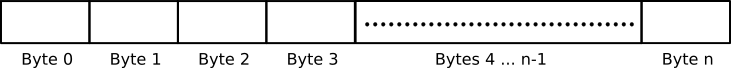
\includegraphics[width=0.75000\textwidth]{Figures/x86-ch/memory-physical-view.png}
\caption{The Physical View of the Memory. The Size of it is
\lstinline!n! Bytes.}\label{fig:memory_physical_view}
\end{figure}

When we say \emph{physical} we mean the actual hardware, that is, when
the maximum capacity of the hardware of the main memory (RAM) is
\lstinline!1MB! then the physical address space of the machine is up to
\lstinline!1MB!. On the other hand, when we say \emph{logical} that
means it doesn't necessarily represents or obeys the way the actual
hardware works on, instead it is a hypothetical way of something that
doesn't exist in the real world (the hardware). To make the
\emph{logical} view of anything works, it should be mapped into the real
\emph{physical} view, that is, it should be somehow translated for the
physical hardware to be understood, this mapping is handled by the
software or sometimes special parts of the hardware.

Now, for the following discussion, let me remind you that the memory
address is just a numerical value, it is just a number. When I discuss
the memory address as a mere number I call it \emph{memory address
value} or \emph{the value of memory address}, while the term
\emph{memory address} keeps its meaning, which is a unique identifier
that refers to a specific location (cell) in the main memory.

The values of memory addresses are used by the processor all the time to
be able to perform its job, and when it is executing some instructions
that involve the main memory (e.g.~reading a content from some memory
location or dealing with program counter), the related values of memory
addresses are stored temporarily on the registers of the processor, due
to that, the length of a memory address value is bounded to the size of
the processor's registers, so, in \lstinline!32-bit! environments, where
the size of the registers is usually \lstinline!32-bit!, the length of
the memory address value is \textbf{always} \lstinline!32! bits, why am
I stressing ``always'' here? Because even if less than \lstinline!32!
bits is enough to represent the memory address value, it will be
represented in \lstinline!32! bits though, for example, assume the
memory address value \lstinline!1!, in binary, the value \lstinline!1!
can be represented by only \lstinline!1 bit! and no more, but in
reality, when it is stored (and handled) by the \lstinline!32-bit!
processor, it will be stored as the following sequence of bits.

\begin{lstlisting}[language=C]
00000000 00000000 00000000 00000001
\end{lstlisting}

As you can see, the value \lstinline!1! has been represented in exactly
\lstinline!32! bits, appending zeros to the left doesn't change the
value itself, it is similar to writing a number as \lstinline!0000539!
which is exactly \lstinline!539!.

It has been mentioned earlier that the register size that stores the
values of memory address in order to deal with memory contents affects
the available size of main memory for the system. Take for example the
instruction pointer register, if its size, say, \lstinline!16! bits then
the maximum available memory for code will be \lstinline!64KB!
(\lstinline!64! KB = \lstinline!65536! Bytes / \lstinline!1024!) since
it is the last reachable memory address by the processor for fetching an
instruction. What if the size of the instruction pointer register is
\lstinline!32! bits, then the maximum available memory for code will be
\lstinline!4GB!. Why is that?

To answer this question let's work with decimal numbers first. If I tell
you that you have five blanks, what is the largest decimal number you
can represent in these five blanks? the answer is \lstinline!99999d!. In
the same manner, if you have \lstinline!5! blanks, what is the largest
binary number you can represent in these 5 blanks? it is
\lstinline!11111b! which is equivalent to \lstinline!31d!, the same
holds true for the registers that store the value of memory addresses,
given the size of such register is \lstinline!16! bits, then there is
\lstinline!16! blanks, and the largest binary number that can be
represented in those \lstinline!16! blanks is
\lstinline!11111111 11111111b! or in hexadecimal \lstinline!FF FFh!,
which is equivalent to \lstinline!65535d!, that means the last byte a
register of size \lstinline!16! bits can refer to is the byte number
\lstinline!65535d! because it is the largest value this register can
store and no more, which leads to the maximum size of main memory this
register can handle, it is \lstinline!65535 bytes! which is equivalent
to \lstinline!64KB! and the same applies on any other size than
\lstinline!16! bits.

\section{x86 Segmentation}\label{x86-segmentation}

The aforementioned view of memory, that is, the \emph{addressable array
of bytes} can be considered as the \emph{physical} view of the main
memory which specifies the mechanism of accessing the data. On top of
this physical view a \emph{logical} view can be created and one example
of logical views is \emph{x86 segmentation}.

In x86 segmentation the main memory is viewed as separated parts called
\emph{segments} and each segment stores a bunch of related data. To
access data inside a segment, each byte can be referred to by its own
\emph{offset}. The running program can be separated into three possible
types of segments in x86, these types are: \emph{code segment} which
stores the code of the program under execution, \emph{data segments}
which store the data of the program and the \emph{stack segment} which
stores the data of program's stack. Segmentation is the default view of
memory in x86 and it's unavoidable and the processor always run with the
mind that the running program is divided into segments, however, most
modern operating system choose to view the memory as the one described
in flat memory model instead of viewing it as segmented areas, to be
able to implement flat memory model in x86 which doesn't allow to
disable segmentation, at least two segments (one for code and one for
data) should be defined in the system, and the size of both segments
should be same as physical memory's size and both of segments start from
the first memory address \lstinline!0! and ends in the last memory
address (memory size - 1), that is, these both segments will overlap.

\begin{figure}
\centering
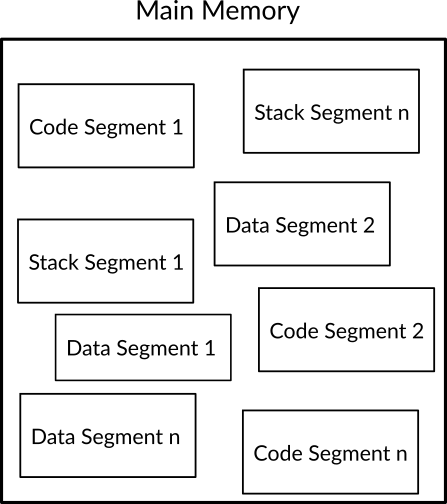
\includegraphics[width=0.35000\textwidth]{Figures/x86-ch/memory-segmented-view.png}
\caption{An Example of The Segmented View of the
Memory}\label{fig:memory_segmented_view}
\end{figure}

\subsection{Segmentation in Real Mode}\label{segmentation-in-real-mode}

For the sake of clarity, let's discuss the details of segmentation under
real mode first. We have said that logical views (of anything) should be
mapped to the physical view either by software or hardware, in this
case, the segmentation view is realized and mapped to the architecture
of the physical main memory by the x86 processor itself, that is, by the
hardware. So, we have a logical view, which is the concept of
segmentation which divides a program into separated segments, and the
actual physical main memory view which is supported by the real RAM
hardware and sees the data as a big array of bytes. Therefore, we need
some tools to implement (map) the logical view of segmentation on top
the actual hardware.

For this purpose, special registers named \emph{segment registers} are
presented in x86, the size of each segment register is \lstinline!16!
bits and they are: \lstinline!CS! which is used to define the code
segment. \lstinline!SS! which is used to define the stack segment.
\lstinline!DS!, \lstinline!ES!, \lstinline!FS! and \lstinline!GS! which
can be used to define data segments, that means each program can have up
to four data segments. Each segment register stores the \emph{starting
memory address} of a segment and here you can start to observe the
mapping between the logical and physical view. In real mode, the size of
each segment is \lstinline!64KB! and as we have said we can reach any
byte inside a segment by using the \emph{offset} of the required byte,
you can see the resemblance between a memory address of the basic view
of memory and an offset of the segmentation view of memory \footnote{The
  concept and term of offset is not exclusive to segmentation, it is
  used on other topics related to the memory.}.

Let's take an example to make the matter clear, assume that we have a
code of some program loaded into the memory and its starting physical
memory address is \lstinline!100d!, that is, the first instruction of
this program is stored in this address and the next instructions are
stored right after this memory address one after another. To reach the
first byte of this code we use the offset \lstinline!0!, so, the whole
physical address of the first byte will be \lstinline!100:0d!, as you
can see, the part before the colon is the starting memory address of the
code and the part after the colon is the offset that we would like to
reach and read the byte inside it. In the same way, let's assume we
would like to reach the offset \lstinline!33!, which means the byte
\lstinline!34! inside the loaded code, then the physical address that we
are trying to reach is actually \lstinline!100:33d!. To make the
processor handle this piece of code as the \emph{current} code segment
then its starting memory address should be loaded into the register
\lstinline!CS!, that is, setting the value \lstinline!100d! to
\lstinline!CS!, so, we can say in other words that \lstinline!CS!
contains the starting memory address of currently executing code segment
(for short: current code segment).

As we have said, the x86 processor always run with the mind that the
segmentation is in use. So, let's say it is executing the following
assembly instruction \lstinline!jmp 150d! which jumps to the address
\lstinline!150d!. What really happens here is that the processor
consider the value \lstinline!150d! as an offset instead of a full
memory address, so, what the instruction requests from the processor
here is to jump to the offset \lstinline!150! which is inside the
current code segment, therefore, the processor is going to retrieve the
value of the register \lstinline!CS! to know what is the starting memory
address of the currently active code segment and append the value
\lstinline!150! to it. Say, the value of \lstinline!CS! is
\lstinline!100!, then the memory address that the processor is going to
jump to is \lstinline!100:150d!.

This is also applicable on the internal work of the processor, do you
remember the register \lstinline!IP! which is the instruction pointer?
It actually stores the offset of the next instruction instead of the
whole memory address of the instruction. Any call (or jump) to a code
inside the same code segment of the caller is known as \emph{near call
(or jump)}, otherwise is it a \emph{far call (or jump)}. Again, let's
assume the current value of \lstinline!CS! is \lstinline!100d! and you
want to call a label which is on the memory location \lstinline!900:1d!,
in this situation you are calling a code that reside in a different code
segment, therefore, the processor is going to take the first part of the
address which is\lstinline!900d!, loads it to \lstinline!CS! then loads
the offset \lstinline!1d! in \lstinline!IP!. Because this call caused
the change of \lstinline!CS! value to another value, it is a far call.

The same is exactly applicable to the other two types of segments and of
course, the instructions deal with different segment types based on
their functionality, for example, you have seen that \lstinline!jmp! and
\lstinline!call! deal the code segment in \lstinline!CS!, that's because
of their functionality which is related to the code. Another example is
the instruction \lstinline!lodsb! which deals with the data segment
\lstinline!DS!, the instruction \lstinline!push! deals with the stack
segment \lstinline!SS! and so on.

\subsubsection{Segmentation Used in the
Bootloader}\label{segmentation-used-in-the-bootloader}

In the previous chapter, when we wrote the bootloader, we have dealt
with the segments. Let's get back to the source code of the bootloader,
you remember that the firmware loads the bootloader on the memory
location \lstinline!07C0h! and because of that we started our bootloader
with the following lines.

\begin{lstlisting}
    mov ax, 07C0h
    mov ds, ax
\end{lstlisting}

Here, we told the processor that the data segment of our program (the
bootloader) starts in the memory address \lstinline!07C0h! \footnote{Yes,
  all segments can be on the same memory location, that is, there is a
  \lstinline!64KB! segment of memory which is considered as the
  currently active code segment, data segment and stack segment. We have
  already mentioned that when we have discussed how to implement
  flat-memory model on x86.}, so, if we refer to the memory to read or
write \textbf{data}, the processor starts with the memory address
\lstinline!07C0h! which is stored in the data segment register
\lstinline!ds! and then it appends the offset that we are referring to,
in other words, any reference to data by the code being executed will
make the processor to use the value in data segment register as the
beginning of the data segment and the offset of referred data as the
rest of the address, after that, this physical memory address of the
referred data will be used to perform the instruction. An example of
instructions that deal with data in our bootloader is the line
\lstinline!mov si, title_string!.

Now assume that BIOS has set the value of \lstinline!ds! to
\lstinline!0! (it can be any other value) and jumped to our bootloader,
that means the data segment in the system now starts from the physical
memory address \lstinline!0! and ends at the physical memory address
\lstinline!65535! since the maximum size of a segment in real-mode is
64KB. Now let's take the label \lstinline!title_string! as an example
and let's assume that its offset in the binary file of our bootloader is
\lstinline!490!, when the processor starts to execute the line
\lstinline!mov si, title_string! \footnote{Which loads the physical
  memory address of \lstinline!title_string! to the register
  \lstinline!si!.} it will, somehow, figures that the offset of
\lstinline!title_string! is \lstinline!490! and based on the way that
x86 handles memory accesses the processor is going to think that we are
referring to the physical memory address \lstinline!490! since the value
of \lstinline!ds! is \lstinline!0!, but in reality, the correct physical
memory address of \lstinline!title_string! is the offset \lstinline!490!
\textbf{inside} the memory address \lstinline!07C0h! since our
bootloader is loaded into this address and not the physical memory
address \lstinline!0!, so, to be able to reach to the correct addresses
of the data that we have defined in our bootloader and that are loaded
with the bootloader starting from the memory address \lstinline!07C0h!
we need to tell the processor that our data segment starts from
\lstinline!07C0h! and with any reference to data, it should calculate
the offset of that data starting from this physical address, and that
exactly what these two lines do, in other words, change the current data
segment to another one which starts from the first place of our
bootloader.

The second use of the segments in the bootloader is when we tried to
load the kernel from the disk by using the BIOS service
\lstinline!13h:02h! in the following code.

\begin{lstlisting}
    mov ax, 0900h
    mov es, ax
    
    mov ah, 02h
    mov al, 01h
    mov ch, 0h
    mov cl, 02h
    mov dh, 0h
    mov dl, 80h
    mov bx, 0h
    int 13h
\end{lstlisting}

You can see here, we have used the other data segment \lstinline!ES! to
define a new data segment that starts from the memory address
\lstinline!0900h!, we did that because the BIOS service
\lstinline!13h:02h! loads the required content (in our case the kernel)
to the memory address \lstinline!ES:BX!, for that, we have defined the
new data segment and set the value of \lstinline!bx! to \lstinline!0h!.
That means the code of the kernel will be loaded on
\lstinline!0900:0000h! and because of that, after loading the kernel
successfully we have performed a far jump.

\begin{lstlisting}
jmp 0900h:0000
\end{lstlisting}

Once this instruction is executed, the value of \lstinline!CS! will be
changed from the value \lstinline!07C0h!, where the bootloader resides,
to the value \lstinline!0900h! where the kernel resides and the value of
\lstinline!IP! register will be \lstinline!0000! then the execution of
the kernel is going to start.

\subsection{Segmentation in Protected
Mode}\label{segmentation-in-protected-mode}

The fundamentals of segmentation in protected mode is exactly same as
the ones explained in real mode, but it has been extended to provide
more features such as \emph{memory protection}. In protected mode, a
table named \emph{global descriptor table} (\lstinline!GDT!) is
presented, this table is stored in the main memory and its starting
memory address is stored in the special purpose register
\lstinline!GDTR! as a reference, each entry in this table called a
\emph{segment descriptor} which has the size \lstinline!8! bytes and
they can be referred to by an index number called \emph{segment
selector} \footnote{This is a \textbf{relaxed} definition of segment
  selector, a more accurate one will be presented later.} which is the
offset of the entry inside \lstinline!GDT! table, For example, the
offset of the first entry in \lstinline!GDT! is \lstinline!0!, and
adding this offset with the value of \lstinline!GDTR! gives us the
memory address of that entry, however, the first entry of
\lstinline!GDT! should not be used by the operating system.

An entry of \lstinline!GDT! (a segment descriptor), defines a segment
(of any type) and has the information that is required by the processor
to deal with that segment. The starting memory address of the segment is
stored in its descriptor \footnote{In real mode, the starting address of
  the segment is stored directly on the corresponding segment register
  (e.g. \lstinline!CS! for code segment).}, also, the size (or limit) of
the segment. The segment selector of the currently active segment should
be stored in the corresponding segment register.

To clarify the matter, consider the following example. Let's assume we
are currently running two programs and their code are loaded into the
main memory and we would like to separate these two pieces of code into
a couple of code segments. The memory area \lstinline!A! contains code
of the first program and starts from the memory address \lstinline!800!
while the memory area \lstinline!B! contains the code of the second
program\lstinline!B! and starts in the memory address \lstinline!900!.
Assume that the starting memory address of \lstinline!GDT! is
\lstinline!500! which is already loaded in \lstinline!GDTR!.

To make the processor consider \lstinline!A! and \lstinline!B! as code
segments we should define a segment descriptor for each one of them. We
already know that the size of a segment descriptor is \lstinline!8!
bytes, so, if we define a segment descriptor for the segment
\lstinline!A! as entry \lstinline!1! (remember that the entries on
\lstinline!GDT! starts from zero) then its offset (segment selector) in
\lstinline!GDT! will be \lstinline!8! (\lstinline!1 * 8!), the segment
descriptor of \lstinline!A! should contain the starting address of
\lstinline!A! which is \lstinline!800!, and we will define the segment
descriptor of \lstinline!B! as entry \lstinline!2! which means its
offset (segment selector) will be \lstinline!16! (\lstinline!2 * 8!).

Let's assume now that we want the processor to execute the code of
segment \lstinline!A!, we already know that the processor consults the
register \lstinline!CS! to decide which code segment is currently active
and should be executed next, for that, the \textbf{segment selector} of
code segment \lstinline!A! should be loaded in \lstinline!CS!, so the
processor can start executing it. In real mode, the value of
\lstinline!CS! and all other segment registers was a memory address, on
the other hand, in protected mode, the value of \lstinline!CS! and all
other segment registers is a segment selector.

In our situation, the processor takes the segment selector of
\lstinline!A! from \lstinline!CS! which is \lstinline!8! and starting
from the memory address which is stored in \lstinline!GDTR! it walks
\lstinline!8! bytes, so, if \lstinline!GDTR = 500!, the processor will
find the segment descriptor of \lstinline!A! in the memory address
\lstinline!508!. The starting address of \lstinline!A! will be found in
its segment descriptor and the processor can use it with the value of
register \lstinline!EIP! to execute \lstinline!A!'s code. Let's assume a
far jump is occurred from \lstinline!A! to \lstinline!B!, then the value
of \lstinline!CS! will be changed to the segment selector of
\lstinline!B! which is \lstinline!16!.

\subsubsection{The Structure of Segment
Descriptor}\label{the-structure-of-segment-descriptor}

A segment descriptor is an \lstinline!8! bytes entry of global
descriptor table which stores multiple \emph{fields} and \emph{flags}
that describe the properties of a specific segment in the memory. With
each memory reference to any segment, the processor is going to consult
the descriptor that describes the segment in question to obtain basic
information like starting memory address of this segment.

Beside the basic information, a segment descriptor stores information
the helps in memory protection, due to that, segmentation in x86
protected-mode is considered as a way for memory protection and not a
mere logical view of the memory, so each memory reference is being
monitored by the processor.

By using those properties that are related to memory protection, the
processor will be able to protect the different segments on the system
from each other and not letting some less privileged to call a code or
manipulate data which belong to more privileged area of the system, a
concrete example of that is when a userspace software (e.g.~Web Browser)
tries to modify an internal data structure in the kernel.

In the following subsections, each field and flag of segment descriptor
will be explained, but before getting started we need to note that in
here and in Intel's official x86 manual the term \emph{field} is used
when the size of the value that should be stored in the descriptor is
\textbf{more than} \lstinline!1! bit, for example the segment's starting
memory address is stored in \lstinline!4! bytes, then the place where
this address is stored in the descriptor is called a field, otherwise
when the term \emph{flag} is used that means the size of the value is
\lstinline!1! bit.

\paragraph{Segment's Base Address and
Limit}\label{segments-base-address-and-limit}

The most important information about a segment is its starting memory
address, which is called the \emph{base address} of a segment. In real
mode, the base address was stored in the corresponding segment register
directly, but in protected mode, where we have more information about a
segment than mere base address, this information is stored in the
descriptor of the segment \footnote{Reminder: In protected mode, the
  corresponding segment register stores the selector of the currently
  active segment.}.

When the currently running code refers to a memory address to read from
it, write to it (in the case of data segments) or call it (in the case
of code segments) it is actually referring to a specific segment in the
system \footnote{And it \textbf{should}, since segmentation is enabled
  by default in x86 and cannot be disabled.}. For the simplicity of next
discussions, we call this memory address, which is referenced by the
currently running code, the \emph{generated memory address} because, you
know, it is generated by the code.

Any generated memory address in x86 architecture is not an actual
physical memory address \footnote{Remember our discussion of the
  difference between our logical view of the memory (e.g.~segmentation)
  and the actual physical hardware}, that means, if you hypothetically
get a generated memory address and try to get the content of its
physical memory location, the obtained data will not be same as the data
which is required by the code. Instead, a generated memory address is
named by Intel's official manual a \emph{logical memory address}
because, you know, it is not real memory address, \textbf{it is}
logical. Every logical memory address refers to some byte in a specific
segment in the system, and to be able to obtain the data from the actual
physical memory, this logical memory address should be \emph{translated}
to a \emph{physical memory address} \footnote{We can see here how
  obvious the mapping between the logical view of the memory and the
  real-world memory.}.

The logical memory address in x86 may pass \textbf{two} translation
processes instead of one in order to obtain the physical memory address.
The first address translation is performed on a logical memory address
to obtain a \emph{linear memory address} which is another not real and
not physical memory address which is there in x86 architecture because
of paging feature. If paging \footnote{Don't worry about paging right
  now. It will be discussed later in this book. All you need to know now
  is that paging is another logical view of the memory. Paging is
  disabled by default in x86 which makes it an optional feature unlike
  segmentation.} is enabled in the system, a second translation process
takes place on this linear memory address to obtain the real physical
memory address. If paging is disabled, the linear memory address which
is generated by the first translation process is same as the physical
memory address. We can say that the first translation is there in x86
due to the segmentation view of memory, while the second translation is
there in x86 due to the paging view of memory.

\begin{figure}
\centering
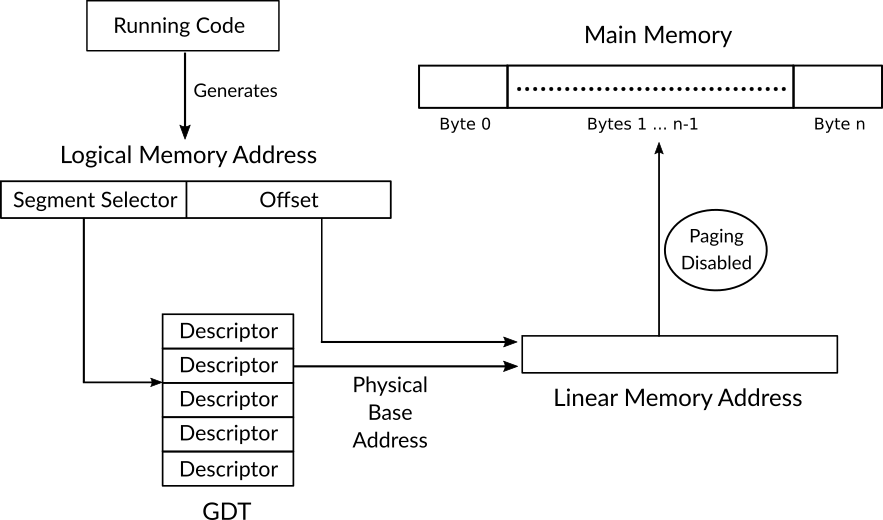
\includegraphics[width=0.90000\textwidth]{Figures/x86-ch/logical-memory-address-translation.png}
\caption{Shows How a Logical Memory Address is Translated to a Linear
Memory Address (Which Represents a Physical Address when Paging is
Disabled).}\label{fig:logical_memory_address_translation}
\end{figure}

For now, our focus will be on the translation from a logical memory
address to a linear memory address which is same as the physical memory
address since paging feature is disabled by default in x86. Each logical
memory address consists of two parts, a \lstinline!16! bits segment
selector and a \lstinline!32! bits offset. When the currently running
code generates a logical memory address (for instance, to read some data
from memory) the processor needs to perform the translation process to
obtain the physical memory address as the following. First, it reads the
value of the register \lstinline!GDTR! which contains the starting
physical memory address of \lstinline!GDT!, then it uses the
\lstinline!16-bit! segment selector in the generated logical address to
locate the descriptor of the segment that the code would like to read
the data from, inside segment's descriptor, the physical base address
(the starting physical address) of the requested segment can be found,
the processor obtains this base address and adds the \lstinline!32-bit!
offset from the logical memory address to the base address to obtain the
last result, which is the linear memory address.

During this operation, the processor uses the other information in the
segment descriptor to enforce the policies of memory protection. One of
these policies is defined by the \emph{limit} of a segment which
specifies its size, if the generated code refers to an offset which
exceeds the limit of the segment, the processor should stop this
operation. For example, assume hypothetically that the running code has
the privilege to read data from data segment \lstinline!A! and in the
physical memory another data segment \lstinline!B! is defined right
after the limit of \lstinline!A!, which means if we can exceed the limit
of \lstinline!A! we will able to access the data inside \lstinline!B!
which is a critical data segment that stores kernel's internal data
structures and we don't want any code to read from it or write to it in
case this code is not privileged to do so. This can be achieved by
specifying the limit of \lstinline!A! correctly, and when the
unprivileged code tries maliciously to read from \lstinline!B! by
generating a logical memory address that has an offset which exceeds the
limit of \lstinline!A! the processor prevents the operation and protects
the content of segment \lstinline!B!.

The limit, or in other words, the size of a given segment is stored in
the \lstinline!20! bits \emph{segment limit field} of that segment
descriptor and how the processor interprets the value of segment limit
field depends on the \emph{granularity flag} (G flag) which is also
stored in the segment's descriptor, when the value of this flag is
\lstinline!0! then the value of the limit field is interpreted as bytes,
let's assume that the limit of a given segment is \lstinline!10! and the
value of granularity flag is \lstinline!0!, that means the size of this
segment is \lstinline!10! \textbf{bytes}. On the other hand, when the
value of granularity flag is \lstinline!1!, the value of segment limit
field will be interpreted as of \lstinline!4KB! units, for example,
assume in this case that the value of limit field is also \lstinline!10!
but G flag = \lstinline!1!, that means the size of the segment will be
\lstinline!10! of \lstinline!4KB! units, that is, \lstinline!10 * 4KB!
which gives us \lstinline!40KB! which equals \lstinline!40960! bytes.

Because the size of segment limit field is \lstinline!20! bits, that
means the maximum numeric value it can represent is
\lstinline!2^20 = 1,048,576!, which means if G flag equals \lstinline!0!
then the maximum size of a specific segment can be \lstinline!1,048,576!
\textbf{bytes} which equals \lstinline!1MB!, and if G flag equals
\lstinline!1! then the maximum size of a specific segment can be
\lstinline!1,048,576! of \lstinline!4KB! units which equals
\lstinline!4! \textbf{GB}.

Getting back to the structure of descriptor, the bytes \lstinline!2!,
\lstinline!3! and \lstinline!4! of the descriptor store the \emph{least
significant bytes} of segment's base address and the byte \lstinline!7!
of the descriptor stores the \emph{most significant byte} of the base
address, the total is \lstinline!32! bits for the base address. The
bytes \lstinline!0! and \lstinline!1! of the descriptor store the
\emph{least significant bytes} of segment's limit and byte \lstinline!6!
stores the \emph{most significant byte} of the limit. The granularity
flag is stored in the most significant \textbf{bit} of the the byte
\lstinline!6! of the descriptor.

Before finishing this subsection, we need to define the meaning of
\emph{least significant} and \emph{most significant} byte or bit. Take
for example the following binary sequence which may represent anything,
from a memory address value to a \lstinline!UTF-32! character.

\textbf{0}111 0101 0000 0000 0000 0000 0100 110\emph{1}

You can see the first bit from left is on bold format and its value is
\lstinline!0!, based on its position in the sequence we call this bit
the \emph{most significant bit} or \emph{high-order bit}, while the last
bit on the right which is in italic format and its value is
\lstinline!1! is known as \emph{least significant bit} or
\emph{low-order bit}. The same terms can be used on byte level, given
the same sequence with different formatting.

\textbf{0111 0101} 0000 0000 0000 0000 \emph{0100 1101}

The first byte (\lstinline!8! bits) on the left which is in bold format
and its value is \lstinline!0111 0101! is known as \emph{most
significant byte} or \emph{high-order byte} while the last byte on the
right which is on italic format and its value is \lstinline!0100 1101!
is known as \emph{least significant byte} or \emph{low-order byte}.

Now, imagine that this binary sequence is the base address of a segment,
then the least significant \lstinline!3! bytes of it will be stored in
bytes \lstinline!2!, \lstinline!3! and \lstinline!4! of the descriptor,
that is, the following binary sequence.

\begin{lstlisting}
0000 0000 0000 0000 0100 1101
\end{lstlisting}

While the most significant byte of the binary sequence will be stored in
the \lstinline!7th! byte of the descriptor, that is, the following
binary sequence.

\begin{lstlisting}
0111 0101
\end{lstlisting}

\paragraph{Segment's Type}\label{segments-type}

Given any binary sequence, it doesn't have any meaning until some
context is added. For example, what does the binary sequence
\lstinline!1100 1111 0000 1010! represents? It could represent anything,
a number, characters, pixels on an image or even all of them based on
how its user interprets it. When an agent (e.g.~a bunch of code in
running software or the processor) works with a binary sequence, it
should know what does this binary sequence represent to be able to
perform useful tasks. In the same manner, when a segment is defined, the
processor (the agent) should be told how to interpret the content inside
this segment, that is, the type of the segment should be known by the
processor.

Till this point, you probably noticed that there is at least two types
of segments, code segment and data segment. The content of the former
should be machine code that can be executed by the processor to perform
some tasks, while the content of the latter should be data (e.g.~values
of constants) that can be used by a running code. These two types of
segments (code and data) belong to the category of \emph{application
segments}, there is another category of segment types which is the
category of \emph{system segments} and it has many different segment
types belong to it.

Whether a specific segment is an application or system segment, this
should be mentioned in the descriptor of the segment in a flag called
\emph{S flag} or \emph{descriptor type flag} which is the fifth
\textbf{bit} in \textbf{byte} number \lstinline!5! of the segment
descriptor. When the value of S flag is \lstinline!0!, then the segment
is considered as a system segment, while it is considered as an
application segment when the value of S flag is \lstinline!1!. Our
current focus is on the latter case.

As we have mentioned before, an application segment can be either code
or data segment. Let's assume some application segment has been
referenced by a currently running code, the processor is going to
consult the descriptor of this segment, and by reading the value of S
flag (which should be \lstinline!1!) it will know that the segment in
question is an application segment, but which of the two types? Is it a
code segment or data segment? To answer this question for the processor,
this information should be stored in a field called \emph{type field} in
the segment's descriptor.

Type field in segment descriptor is the first \lstinline!4! bits
(nibble) of the fifth byte and the most significant bit specifies if the
application segment is a code segment (when the value of the bit is
\lstinline!1!) or a data segment (when the value of the bit is
\lstinline!0!). Doesn't matter if the segment is a code or data segment,
in the both cases the least significant bit of type field indicates if
the segment is \emph{accessed} or not, when the value of this flag is
\lstinline!1!, that means the segment has been written to or read from
(AKA: accessed), but if the value of this flag is \lstinline!0!, that
means the segment has not been accessed. The value of this flag is
manipulated by the processor in one situation only, and that's happen
when the selector of the segment in question is loaded into a segment
register. In any other situation, it is up to the operating system to
decide the value of accessed flag. According to Intel's manual, this
flag can be used for virtual memory management and for debugging.

\subparagraph{Code Segment Flags}\label{code-segment-flags}

When the segment is a code segment, the second most significant bit
(tenth bit) is called \emph{conforming flag} (also called \lstinline!C!
flag) while the third most significant bit (ninth bit) called
\emph{read-enabled flag} (also called \lstinline!R! flag.). Let's start
our discussion with the simplest among those two flags which is the
read-enabled flag. The value of this flag indicates how the code inside
the segment in question can be used, when the value of read-enabled flag
is \lstinline!1! \footnote{Which means \textbf{do} enable read, since
  \lstinline!1! is equivalent to \lstinline!true! in the context of
  flags.}, that means the content of the code segment can be executed
\textbf{and} read from, but when the value of this flag is \lstinline!0!
\footnote{Which means \textbf{don't} enable read.} that means the
content of the code segment can be \textbf{only} executed and cannot
read from. The former option can be useful when the code contains data
inside it (e.g.~constants) and we would like to provide the ability of
reading this data. When read is enabled for the segment in question, the
selector of this segment can also be loaded into one of data segment
registers \footnote{Which makes sense, enabling reads from a code
  segment means it contains data also.}.

The conforming flag is related to the privilege levels that we had an
overview about them previously in this chapter. When a segment is
conforming, in other words, the value of conforming flag is
\lstinline!1!, that means a code which runs in a less-privileged level
can call this segment which runs in a higher privileged level while
keeping the current privilege level of the environment same as the one
of the caller instead of the callee.

For example, let's assume for some reason a kernel's designer decided to
provide simple arithmetic operations (such as addition and subtraction)
for user applications from the kernel code, that is, there is no other
way to perform these operations in that system but this code which is
provided by the kernel. As we know, kernel's code should run in
privilege level \lstinline!0! which is the most-privileged level, and
let's assume a user application which runs in privilege level
\lstinline!3!, a less-privileged level, needs to perform an addition
operation, in this case a kernel code, which should be protected by
default from being called by less-privileged code, should be called to
perform the task, this can only realized if the code of addition
operation is provided as a conforming segment, otherwise the processor
is going to stop this action where a less-privileged code calls a
more-privileged code.

Also you should note that the code of addition operation is going to run
in privilege level \lstinline!3! although it is a part of the kernel
which runs in privilege level \lstinline!0! and that's because of the
original caller which runs in the privilege level \lstinline!3!.
Furthermore, although conforming segment can be called by a
less-privilege code (e.g.~user application calls the kernel), the
opposite cannot be done (e.g.~the kernel calls a user application's
code) and the processor is going to stop the operation.

\subparagraph{Data Segment Flags}\label{data-segment-flags}

When the segment is data segment, the second most significant bit (tenth
bit) is called expansion-direction flag (also called \lstinline!E! flag)
while the third most significant bit (ninth bit) is called write-enabled
flag (also called \lstinline!W! flag). The latter one gives us the
ability to make some data segment a read-only when its value is
\lstinline!0!, or we can make a data segment both \textbf{writable} and
readable by setting the value of write-enabled flag to \lstinline!1!.

While the expansion-direction flag and its need will be examined in
details when we discuss x86 run-time stack in this chapter, what we need
to know right now is that when the value of this flag is \lstinline!0!,
the data segment is going to expand \textbf{up} (in Intel's terms), but
when the value of this flag is \lstinline!1!, the data segment is going
to expand \textbf{down} (in Intel's terms).

A last note about data segments is that all of them are
\textbf{non-conforming}, that is, a less-privileged code cannot access a
data segment in a more-privileged level. Furthermore, all data segments
can be accessed by a more-privileged code.

\paragraph{Segment's Privilege Level}\label{segments-privilege-level}

In our previous discussions, we have stated that a specific segment
should belong to a privilege level and based on this privilege level the
processor decides the protection properties of the segment in question,
for example, whether that segment is a kernel-mode or user-mode segment
and which privilege level a running code should belong to in order to be
able to reach to this segment

A field called \emph{descriptor privilege level} (DPL) in segment
descriptor is where the operating system should set the privilege level
of a given segment. The possible values of this field, as we know, are
\lstinline!0!, \lstinline!1!, \lstinline!2! and \lstinline!3!, we have
already discussed the meanings of these values previously in this
chapter. Descriptor privilege level field occupies the second and third
most significant bits of byte \lstinline!5! in a descriptor.

\paragraph{Segment's Present}\label{segments-present}

One of common operations that is performed in a running system is
loading data from secondary storage (e.g.~hard disk) into the memory and
one example of that is loading a program code into the memory when the
user of the system request to run an instance of a program, so, creating
a new segment descriptor (hence, creating new segment in the memory) for
this data may precede the completion of loading the data into the main
memory, therefore, there could be some segment descriptors in the system
that points to memory locations that don't contain the real data yet.

In this case, we should tell the processor that the data in the memory
location that a specific descriptor points to is not the real data, and
the real segment is not presented in the memory yet, this helps the
processor to generate error when some code tries to access \footnote{We
  use the term \emph{access} here for both types of application
  segments. While this term is valid for data segment, we mean
  \emph{execute} for code segment.} the segment's data. To tell the
processor whether a segment is presented in the memory or not,
\emph{segment-present flag} (P flag) can be used, when its value is
\lstinline!1! that means the segment is present in memory, while the
value \lstinline!0! means the segment is not present in memory, this
flag is the most significant bit of byte \lstinline!5! of a descriptor.

\paragraph{Other Flags}\label{other-flags}

We have covered all segment's descriptor fields and flags but three
flags. The name of the first one changes depending on the type of the
segment and it occupies the second most significant bit in the byte
\lstinline!6!. When the segment in question is a code segment, this flag
is called \emph{default operation size} (D flag). When the processor
executes the instructions it uses this flag to decide the length of the
operands, depending on the currently executing instruction, if the value
of D flag is \lstinline!1! the processor is going to assume the operand
has the size of \lstinline!32! bits if it is a memory address, and
\lstinline!32! bits or \lstinline!8! bits if it is not a memory address.
If the value of D flag is \lstinline!0! the processor is going to assume
the operand has the size of \lstinline!16! bits if it is a memory
address, and \lstinline!16! bits or \lstinline!8! bits operand if it is
not a memory address.

When the segment in question is a stack segment \footnote{The processor
  knows it is a stack segment if the segment selector is loaded into
  stack segment selector register \lstinline!SS!}, the same flag is
called \emph{default stack pointer size} (B flag), and it decides the
size of the memory address (as a value) which points to the stack, this
memory address is known as \emph{stack pointer} and it is being used
implicitly by stack instructions such as \lstinline!push! and
\lstinline!pop!. When the value of B flag is \lstinline!1!, then the
size of stack pointer will be \lstinline!32! bits and its value will be
stored in the register \lstinline!ESP! (rather then \lstinline!SP!),
When the value of B flag is \lstinline!0!, then the size of stack
pointer will be \lstinline!16! bits and its value will be stored in the
register \lstinline!SP! (rather then \lstinline!ESP!).

When the segment in question is a data segment that grows upward, this
flag is called \emph{upper bound flag} (B flag), when its value is
\lstinline!1! the maximum possible size of the segment will be
\lstinline!4GB!, otherwise, the maximum possible size of the segment
will be \lstinline!64KB!. Anyway, the value of this flag (D/B flag)
\textbf{should} be \lstinline!1! for \lstinline!32-bit! code and data
segments (stack segments are included of course) and it should be
\lstinline!0! for \lstinline!16-bit! code and data segments.

The second flag is known as \emph{64-bit code segment flag} (L flag)
which is the third most significant bit in the byte \lstinline!6! and
from its name we can tell that this flag is related to code segments. If
the value of this flag is \lstinline!1! that means the code inside the
segment in question is a \lstinline!64-bit! code while the value
\lstinline!0! means otherwise \footnote{In terms of Intel's manual:
  \emph{compatibility mode}.}. When we set the value of L flag to
\lstinline!1! the value of D/B flag should be \lstinline!0!.

The final flag is the fourth most significant bit in the byte
\lstinline!6!, the value of this flag has no meaning for the processor,
hence, it will not use it to make any decisions upon the segment in the
question as we have seen on all other flags and fields. On the other
hand, this flag is available for the operating system to use it in
whatever way it needs, or just ignores it by set it to any of possible
values ,\lstinline!0! or \lstinline!1! since it is one bit.

\subsubsection{\texorpdfstring{The Special Register
\texttt{GDTR}}{The Special Register GDTR}}\label{the-special-register-gdtr}

The special register \lstinline!GDTR! stores the base physical address
\footnote{More accurately, the linear address. Refer to discussion of
  memory translation process in this chapter.} of the global descriptor
table, that is, the starting point of \lstinline!GDT! table. Also, the
same register stores the limit (or size) of the table.

\begin{figure}
\centering
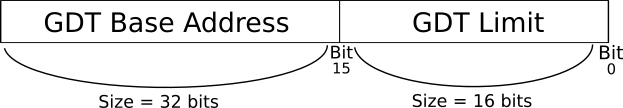
\includegraphics[width=0.50000\textwidth]{Figures/x86-ch/Fig16062021_0.png}
\caption{GDTR Structure}\label{fig:16062021_0}
\end{figure}

To load a value into the register \lstinline!GDTR! the x86 instruction
\lstinline!lgdt!, which stands for \emph{load} global descriptor table,
should be used. This instruction takes one operand which is the whole
value that should be loaded into \lstinline!GDTR!, the structure of this
value should be similar to the structure of \lstinline!GDTR! itself
which is shown in figure \ref{fig:16062021_0}. The figure shows that the
total size of \lstinline!GDTR! is \lstinline!48! bits divided into two
parts. The first part starts from bit \lstinline!0! (the least
significant bit) to bit \lstinline!15!, this part contains the limit of
\lstinline!GDT! table that we would like to load. The size of this part
of \lstinline!GDTR! register is \lstinline!16! bits which can represent
the value \lstinline!65,536! at maximum, that means the maximum size of
\lstinline!GDT! table can be \lstinline!64KB = 65,536 Bytes / 1024!, and
as we know, the size of each of descriptor is \lstinline!8! bytes, that
means the \lstinline!GDT! table can hold \lstinline!8,192! descriptors
at most. The second part of \lstinline!GDTR! starts from bit
\lstinline!16! to bit \lstinline!47! (the most significant bit) and
stores the base memory address of \lstinline!GDT! table that we would
like to load.

\subsubsection{Local Descriptor Table}\label{local-descriptor-table}

The global descriptor table is a system-wide table, in other words, it
is available for every process of the system. In addition to
\lstinline!GDT!, x86 provides us with ability to define \emph{local
descriptor tables} (\lstinline!LDT!) in protected-mode which have the
same functionality and structure of \lstinline!GDT!.

In contrary to \lstinline!GDT! table, multiple \lstinline!LDT! can be
defined in the system, and each one of them can be private to a specific
process that is currently running on the system, also, multiple running
processes can share a single \lstinline!LDT! that is considered private
for them by the kernel and no other processes can reach this given
\lstinline!LDT!. Anyway, how to use \lstinline!LDT! depends on how the
kernel is designed, and while \lstinline!GDT! is required in x86
architecture by default, \lstinline!LDT! on the other hand is optional
and the designer of the kernel is the one who is responsible to decide
whether to use \lstinline!LDT! or not.

Let's assume that we need to create a new \lstinline!LDT! table for
process \lstinline!A! which is currently running on the system, this
\lstinline!LDT! table is already filled with the descriptors that
describe the segments which belong to process \lstinline!A!. The
structure of the descriptors in \lstinline!LDT! is exactly same as the
one that we already described in this chapter. To tell the processor
that a given region of a memory is an \lstinline!LDT! table, a new
segment descriptor should be created in \lstinline!GDT!.

In our previous discussion of \lstinline!S! flag we mentioned that this
flag tells the processor whether a defined segment is an application
segment (S flag = \lstinline!1!) or a system segment (S flag =
\lstinline!0!), the segment of the memory that contains an
\lstinline!LDT! table is considered as a system segment, that is, the
value of \lstinline!S! flag in the descriptor that describes an
\lstinline!LDT! table should be \lstinline!0! and because there are
other types of system segments than \lstinline!LDT! then we should tell
the processor this system segment is an \lstinline!LDT! table, to do
that we should use the type field of the descriptor that we already
mentioned, the value of this field should be \lstinline!0010b!
(\lstinline!2d!) for descriptors that describe an \lstinline!LDT! table,
how the processor can tell which table should currently used for a given
segment \lstinline!GDT! or \lstinline!LDT! will be discussed in the next
subsection.

The x86 instruction \lstinline!lldt! is used to load the \lstinline!LDT!
table that we would like to use now into a special register named
\lstinline!LDTR! which is a \lstinline!16-bit! register that should
contain the segment selector \footnote{More accurate definition of a
  segment selector and its structure in protected-mode is presented in
  the next subsection.} in \lstinline!GDT! of the \lstinline!LDT! table
that we would like to use, in other words, the index of segment
descriptor which describe the \lstinline!LDT! table and which reside in
\lstinline!GDT! as an entry should be loaded into \lstinline!LDTR!
register.

\subsubsection{Segment Selector}\label{segment-selector}

As we know, the index (offset) of the descriptor that the currently
running code needs to use, whether this descriptor defines and code or
data segment, should be loaded into one of segment registers, but how
the can the processor tell if this index which is loaded into a segment
register is an index in the \lstinline!GDT! or \lstinline!LDT!?

\begin{figure}
\centering
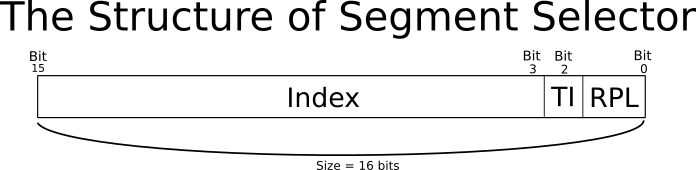
\includegraphics[width=0.50000\textwidth]{Figures/x86-ch/Fig17062021_0.png}
\caption{Segment Selector Structure}\label{fig:17062021_0}
\end{figure}

When we discussed segment selectors previously in this chapter we have
said that our definition of this concept is a \textbf{relaxed}
definition, that is, a simplified one that omits some details. In
reality, the index of a segment descriptor is just one part of a segment
selector, figure \ref{fig:17062021_0} shows the structure of a segment
selector, which is same as the structure of all segment registers
\lstinline!CS!, \lstinline!SS!, \lstinline!DS!, \lstinline!ES!,
\lstinline!FS! and \lstinline!GS!. We can see from the figure that the
size of a segment selector is \lstinline!16! bits and starting from the
least significant bit (bit \lstinline!0!), the first two bits
\lstinline!0! and \lstinline!1! are occupied by field known as
\emph{requester privilege level} (\lstinline!RPL!). Bit \lstinline!2! is
occupied by a flag named \emph{table indicator} (\lstinline!TI!), and
finally, the index of a segment descriptor occupies the field from bit
\lstinline!3! until bit \lstinline!15! of the segment selector. The
index field (descriptor offset) is already well-explained in this
chapter, so we don't need to repeat its details.

The table indicator flag (\lstinline!TI!) is the one which is used by
the processor to tell if the index in the segment selector is an index
in \lstinline!GDT!, when the value of \lstinline!TI! is \lstinline!0!,
or \lstinline!LDT!, when the value is \lstinline!1!. When the case is
the latter, the processor consults the register \lstinline!LDTR! to know
the index of the descriptor that defines the current \lstinline!LDT! in
the \lstinline!GDT! and by using this index, the descriptor of
\lstinline!LDT! is read from \lstinline!GDT! by the processor to fetch
the base memory address of the current \lstinline!LDT!, after that, the
index in the segment selector register can be used to get the required
segment descriptor from the current \lstinline!LDT! by using the latter
base memory address that just been fetched, of course these values are
cached by the processor for quick future access.

In our previous discussions of privilege levels we have discussed two
values, current privilege level (\lstinline!CPL!) which is the privilege
level of the currently executing code and descriptor privilege level
(\lstinline!DPL!) which is the privilege level of a given segment, the
third value which contributes to the privilege level checks in x86 is
\emph{requester privilege level} (\lstinline!RPL!) which is stored in
the segment selector, necessarily, \lstinline!RPL! has four possible
values \lstinline!0!, \lstinline!1!, \lstinline!2! and \lstinline!3!.

To understand the role of \lstinline!RPL! let's assume that a process
\lstinline!X! is running in a user-mode, that is, in privilege level
\lstinline!3!, this process is a malicious process that aims to gain an
access to some important kernel's data structure, at some point of time
the process \lstinline!X! calls a code in the kernel and passes the
segment selector of the more-privileged data segment to it as a
parameter, the kernel code runs in the most privileged level and can
access all privileged data segment by simply loading the required data
segment selector to the corresponding segment register, in this case the
\lstinline!RPL! is set to \lstinline!0! maliciously by process
\lstinline!X!, since the kernel runs on the privilege level
\lstinline!0! and \lstinline!RPL! is \lstinline!0!, the required segment
selector by process \lstinline!X! will be loaded and the malicious
process \lstinline!X! will be able to gain access to the data segment
that has the sensitive data.

To solve this problem, \lstinline!RPL! should be set to the
\textbf{requester} privilege level by the kernel to load the required
data segment, in our example, the requester (the caller) is the process
\lstinline!X! and its privilege level is \lstinline!3! and the current
privilege level is \lstinline!0! since the kernel is running, but
because the caller has a less-privileged level the kernel should set the
\lstinline!RPL! of the required data segment selector to \lstinline!3!
instead of \lstinline!0!, this tells the processor that while the
currently running code in a privilege level \lstinline!0! the code that
called it was running in privilege level \lstinline!3!, so, any attempt
to reach a segment which its selectors \lstinline!RPL! is larger than
\lstinline!CPL! should be denied, in other words, the kernel should not
reach privileged segments in behalf of process \lstinline!X!. The x86
instruction \lstinline!arpl! can be used by the kernel's code to change
the \lstinline!RPL! of the segment selector that has been requested by
less-privileged code to access to the privilege level of the caller, as
in the example of process \lstinline!X!.

\section{x86 Run-time Stack}\label{x86-run-time-stack}

A user application starts its life as a file stored in user's hard disk,
at this stage it does nothing, it is just a bunch of binary numbers that
represent the machine code of this application, when the user decides to
use this application and opens it, the operating system loads this
application into the memory and in this stage this user application
becomes a process, we mentioned before that the term ``process'' is used
in operating systems literature to describe a running program, another
well-known term is \emph{task} which is used by Linux kernel and has the
same meaning.

Typically, the memory of a process is divided into multiple regions and
each one of them stores a different kind of application's data, one of
those regions stores the machine code of the application in the memory,
there are also two important regions of process' memory, the first one
is known as \emph{run-time heap} (or just \textbf{heap} for short) which
provides an area for dynamically allocated objects (e.g.~variables), the
second one is known as \emph{run-time stack} (or \textbf{stack} for
short), it's also known as \emph{call stack} but we are going to stick
to the term run-time stack in our discussions. Please note that the
short names of run-time stack (that is, stack) and run-time heap (that
is, heap) are also names for \textbf{data structures}. As we will see
shortly, a data structure describes a way of storing data and how to
manipulate this data, while in our current context these two terms are
used to represent \textbf{memory regions} of a running process although
the stack (as memory region) uses stack data structure to store the
data. Due to that, here we use the more accurate term \emph{run-time
stack} to refer the memory region and \emph{stack} to refer the data
structure.

Run-time stack is used to store the values of local variables and
function parameters, we can say that the run-time stack is a way to
implement \emph{function's invocation} which describes how function
\lstinline!A! can call function \lstinline!B!, pass to it some
parameters, return back to the same point of code where function
\lstinline!A! called function \lstinline!B! and finally get the returned
value from function \lstinline!B!, the implementation details of these
steps is known as \emph{calling convention} and the run-time stack is
one way of realizing these steps. There are multiple known calling
conventions for x86, different compilers and operating systems may
implement different calling conventions, we are not going to cover those
different methods but what we need to know that, as we said, those
different calling conventions use the run-time stack as a tool to
realize function's invocation. The memory region in x86 which is called
run-time stack uses a data structure called \emph{stack} to store the
data inside it and to manipulate that data.

\subsection{The Theory: Stack Data
Structure}\label{the-theory-stack-data-structure}

Typically, a \emph{data structure} as a concept is divided into two
components, the first one is the way of storing the data in a high-level
terms, a data structure is not concerned about how to store the data in
low-level (e.g as bits, or bytes. In the main memory or on the disk,
etc.). But it answers the question of storing data as a high-level
concept (as we will see in stack example) without specifying the details
of implementation and due to that, they are called \emph{abstract data
structures}. The second component of a data structure is the available
operations to manipulate the stored data. Of course, the reason of the
existence of each data structure is to solve some kind of problem.

In stack data structure, the data will be stored in first-in-last-out
(FILO) manner \footnote{On contrary, \emph{queue data structure} stores
  data in first-in-\textbf{first}-out (FIFO) manner.}, that is, the
first entry which is stored in the stack can be fetched out of the stack
at last. The operations of stack data structure are two: \emph{push} and
\emph{pop} \footnote{That doesn't mean no more operations can be defined
  for a given data structure in the implementation level. It only means
  that the conceptual perspective for a given data structure defines
  those basic operations which reflect the spirit of that data
  structure. Remember that when we start to use x86 run-time stack with
  more operations than \lstinline!push! and \lstinline!pop! later,
  though those other operations are not canonical to the stack data
  structure, but they can be available if the use case requires that
  (and yes they may violate the spirit of the given data structure! We
  will see that later).}, the first one puts some value on the \emph{top
of the stack}, which means that the top of stack always contains the
last value that have been inserted (pushed) into a stack. The latter
operation \lstinline!pop! \textbf{removes} the value which resides on
the top of the stack and returns it to the user, that means the most
recent value that has been \lstinline!push!ed to the stack will be
fetched when we \lstinline!pop! the stack.

\begin{figure}
\centering
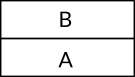
\includegraphics[width=0.35000\textwidth]{Figures/x86-ch/abcd-stack-step1.png}
\caption{A Stack with Two Values \lstinline!A! and \lstinline!B! Pushed
Respectively.}\label{fig:abcd-stack-step1}
\end{figure}

Let's assume that we have the string \lstinline!ABCD! and we would like
to push each character separately into the stack. First we start with
the operation \lstinline!push A! which puts the value \lstinline!A! on
the top of the stack, then we execute the operation \lstinline!push B!
which puts the value \lstinline!B! on top of the value \lstinline!A! as
we can see in the figure \ref{fig:abcd-stack-step1}, that is, the value
\lstinline!B! is now on the top of the stack and not the value
\lstinline!A!, the same is going to happen if we push the value
\lstinline!C! next as you can see in the figure
\ref{fig:abcd-stack-step2} and the same for the value of \lstinline!D!
and you can see the final stack of these four push operations in figure
\ref{fig:abcd-stack-step3}.

\begin{figure}
\centering
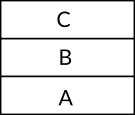
\includegraphics[width=0.35000\textwidth]{Figures/x86-ch/abcd-stack-step2.png}
\caption{A Stack with Three Values \lstinline!A!, \lstinline!B! and
\lstinline!C! Pushed Respectively.}\label{fig:abcd-stack-step2}
\end{figure}

\begin{figure}
\centering
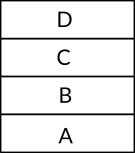
\includegraphics[width=0.35000\textwidth]{Figures/x86-ch/abcd-stack-step3.png}
\caption{A Stack with Four Values \lstinline!A!, \lstinline!B!,
\lstinline!C! and \lstinline!D! Pushed
Respectively.}\label{fig:abcd-stack-step3}
\end{figure}

Now let's assume that we would like to read the values from this stack,
the only way to read data in stack data structure is to use the
operation \lstinline!pop! which, as we have mentioned, removes the value
that resides on the top of the stack and returns it to the user, that
is, the stack data structure in contrary of array data structure
\footnote{Which is implemented by default in most major programming
  languages and know as arrays (in C for example) or lists (as in
  Python)} doesn't have the property of \emph{random access} to the
data, so, if you want to access any data in the stack, you can only use
\lstinline!pop! to do that. That means if you want to read the first
pushed value to the stack, then you need to \lstinline!pop! the stack
\lstinline!n! times, where \lstinline!n! is the number of pushed
elements into the stack, in other words, the size of the stack.

In our example stack, to be able to read the first pushed value which is
\lstinline!A! you need to \lstinline!pop! the stack four times, the
first one removes the value \lstinline!D! from the top of stack and
returns it to the user, which makes the values \lstinline!C! on the top
of stack as you can see in figure \ref{fig:abcd-stack-step2} and if we
execute \lstinline!pop! once again, the value \lstinline!C! will be
removed from the top of the stack and returns it to the user, which
makes the value \lstinline!B! on the top of the stack as you can see in
figure \ref{fig:abcd-stack-step1}, so we need to \lstinline!pop! the
stack two times more the get the first \lstinline!push!ed value which is
\lstinline!A!. This example makes it obvious for us why the stack data
structure is described as first-in-last-out data structure.

The stack data structure is one of most basic data structures in
computer science and there are many well-known applications that can use
stack to solve a specific problem in an easy manner. To take an example
of applications that can use a stack to solve a specific problem let's
get back to our example of \lstinline!push!ing \lstinline!ABCD! into a
stack, character by character and then \lstinline!pop!ping them back,
the input is \lstinline!ABCD! but the output of \lstinline!pop!
operation is \lstinline!DCBA! which is the reverse string of the input,
so, the stack data structure can be used to solve the problem of getting
the reversed string of an input by just pushing it into a stack
character by character and then popping this stack, concatenating the
returned character with the previously returned character, until the
stack becomes empty. Other problems that can be solved easily with stack
are palindrome problem and parenthesis matching problem which is an
important one for a part of programming languages' compilers and
interpreters known as parser.

As you can see in this brief explanation of stack data structure, we
haven't mention any implementation details which means that a specific
data structure is an abstract concept that describes a high-level idea
where the low-level details are left for the implementer.

\subsection{The Implementation: x86 Run-time
Stack}\label{the-implementation-x86-run-time-stack}

Now, with our understanding of the theoretical aspect of stack data
structure, let's see how the run-time stack is implemented in x86
architecture to be used for the objectives that we have mentioned in the
beginning of the subsection. As we have said earlier, the reason of x86
run-time stack's existence is to provide a way to implement function's
invocation, that is, the lifecycle of functions. Logically, we know that
a program consists of multiple functions (or \emph{routines} which is
another term that is used to describe the same thing) and when executing
a program (a process), a number of these functions (not necessarily all
of them) should be called to fulfill the required job.

In run-time context, a function \lstinline!B! starts its life when it's
called by another function \lstinline!A!, so, the function \lstinline!A!
is the \emph{caller}, that is, the function that originated the call,
and the function \lstinline!B! is the \emph{callee}. The caller can pass
a bunch of parameters to the callee which can reach the value of these
parameters while it's running, the callee can define its own local
variables which should not be reached by any other function, that means
that these variables can be removed from the memory once the callee
finishes its job. When the callee finishes its job, it may \emph{return}
some value to the caller \footnote{Some programming languages,
  especially those which are derived from Algol differentiate between a
  \emph{function} which \textbf{should} return a value to the caller,
  and a \emph{procedure} which \textbf{shouldn't} return a value to the
  caller.}. Finally, the run-time platform (the processor in the case of
compiled languages) should be able to know, when the callee finishes,
where is the place of the code that should be executed next, and
logically, this place is the line in the source code of the caller
function which is next to the line that called the callee in the first
place.

In x86, each process has its own run-time stack \footnote{We claim that
  for the purpose of explanation. But actually the matter of separated
  run-time stack for each process is a design decision that the
  operating system's kernel programmer/designer is responsible for.}, we
can imagine this run-time stack as a big (or even small, that depends on
practical factors) memory region that obeys the rules of stack data
structure. This run-time stack is divided into multiple mini-stacks,
more formally, these mini-stacks are called \emph{stack frames}. Each
stack frame is dedicated to \textbf{one} function which has been called
during the execution of the program, once this function exists, its
frame will be removed from the larger process stack, hence, it will be
removed from the memory.

The x86 register \lstinline!EBP! (which is called the \emph{stack frame
base pointer}) contains the starting memory address of the current stack
frame, and the register \lstinline!ESP! (which is called the \emph{stack
pointer}) contains the memory address of the top of the stack. To push a
new item into the run-time stack, an x86 instruction named
\lstinline!push! can be used with the value of the new item as an
operand, this instruction decrements the value of \lstinline!ESP! to get
a new \emph{starting} memory location to put the new value on and to
keep \lstinline!ESP! pointing to the top of the stack, decrementing the
value of \lstinline!ESP! means that the newly pushed items are stored in
a lower memory location than the previous value and that means the
run-time stack in x86 \emph{grows downward} in the memory.

When we need to read the value on the top of the stack and removes this
value from the stack, the x86 instruction \lstinline!pop! can be used
which is going to store the value (which resides on the top of stack) on
the specified location on its operand, this location can be a register
or a memory address, after that, \lstinline!pop! operation increments
the value of \lstinline!ESP!, so the top of stack now refers to the
previous value. Note that the \lstinline!pop! instruction only
increments \lstinline!ESP! to get rid of the popped value and don't
clear it from memory by, for example, writing zeros on its place which
is better for the performance, and this is one of the reasons when you
refer to some random memory location, for example in C pointers, and you
see some weird value that you probably don't remember that you have
stored it in the memory, once upon a time, this value may have been
pushed into the run-time stack and its frame has been removed. This same
practice is also used in modern filesystems for the sake of performance,
when you delete a file the filesystem actually doesn't write zeros in
the place of the original content of the file, instead, it just refer to
its location as a free space in the disk, and maybe some day this
location is used to store another file (or part of it), and this is when
the content of the deleted file are actually cleared from the disk.

Let's get back to x86 run-time stack. To make the matter clear in how
\lstinline!push! and \lstinline!pop! work, let's take an example. Assume
that the current memory address of the top of stack (\lstinline!ESP!) is
\lstinline!102d! and we executed the instruction \lstinline!push A!
where \lstinline!A! is a character encoded in \lstinline!UTF-16! which
means its size is \lstinline!2! bytes (\lstinline!16! bits) and it is
represented in hexadecimal as \lstinline!0x0410!, by executing this
\lstinline!push! instruction the processor is going to subtract
\lstinline!2! from \lstinline!ESP! (because we need to push
\lstinline!2! bytes into the stack) which gives us the new memory
location \lstinline!100d!, then the processor stores the first byte of
\lstinline!UTF-16! \lstinline!A! (\lstinline!0x04!) in the location
\lstinline!100d! and the second byte (\lstinline!0x10!) in the location
\lstinline!101d! \footnote{In fact, x86 is little-endian architecture
  which means that \lstinline!0x10! will be stored in the location
  \lstinline!100d! while \lstinline!0x04! will be stored in the location
  \lstinline!101d! but I've kept the example in the main text as is for
  the sake of simplicity.}, the value of \lstinline!ESP! will be changed
to \lstinline!100d! which now represents the top of the stack.

When we need to \lstinline!pop! the character \lstinline!A! from the top
of the stack, both bytes should be read and \lstinline!ESP! should be
\textbf{incremented} by \lstinline!2!. In this case, the new memory
location \lstinline!100d! can be considered as a \emph{starting}
location of the data because it doesn't store the whole value of
\lstinline!A! but a part of it, the case where the new memory location
is not considered as starting memory location is when the newly pushed
values is pushed as whole in the new memory location, that is, when the
size of this value is \lstinline!1! byte.

\subsection{Calling Convention}\label{calling-convention}

When a function \lstinline!A! needs to call another function
\lstinline!B!, then as a first step \lstinline!A! (the caller) should
push into the stack the parameter that should be passed to \lstinline!B!
(the callee), that means the parameters of \lstinline!B! will be stored
on the stack frame of \lstinline!A!, when pushing the parameters, they
are pushed in a reversed order, that is, the last parameter is pushed
first and so on. Then the x86 instruction \lstinline!call! can be used
to jump to function \lstinline!B! code. Before jumping to the callee
code, the instruction \lstinline!call! pushes the current value of
\lstinline!EIP! (this is, the returning memory address) onto the stack,
at this stage, the value of \lstinline!EIP! is the memory address of the
instruction of \lstinline!A! which is right after \lstinline!call B!
instruction, pushing this value into the stack is going to help the
processor later to decide which instruction of the running code should
be executed after the function \lstinline!B! finishes. Now, assume that
the function \lstinline!B! receives three parameters \lstinline!p1!,
\lstinline!p2! and \lstinline!p3!, the figure \ref{fig:call-conv-1}
shows the run-time stack at the stage where \lstinline!call! instruction
has been performed its first step (pushing \lstinline!EIP!). Also, the
following assembly code shows how \lstinline!A! pushes the parameters
then calls \lstinline!B!, as you can see, after \lstinline!B! finishes
and the execution of \lstinline!A! resumes, the value of \lstinline!EAX!
is moved to \lstinline!ECX! and this line is just an example and not a
part of calling convention.

\begin{lstlisting}
A:
; A's Code Before Calling B

push p3
push p2
push p1
call B
mov ecx, eax

; Rest of A's Code
\end{lstlisting}

\begin{figure}
\centering
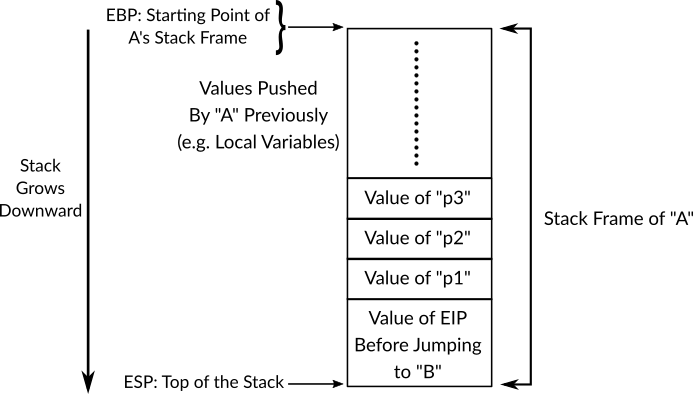
\includegraphics[width=0.55000\textwidth]{Figures/x86-ch/call-conv-1.png}
\caption{Run-time Stack Before Jumping to Function \lstinline!B!
Code}\label{fig:call-conv-1}
\end{figure}

When the processor starts executing function \lstinline!B!, or any other
function, it's the job of the function to create its own stack frame,
therefore, the first piece of any function's code should be responsible
for creating a new stack frame, this happens by moving the value of
\lstinline!ESP! (the memory address of the top of stack) to the register
\lstinline!EBP!, but before that, we should not lose the previous value
of \lstinline!EBP! (the starting memory address of the caller's stack
frame), this value will be needed when the callee \lstinline!B!
finishes, so, the function \lstinline!B! should push the value of
\lstinline!EBP! onto the stack and only after that it can change
\lstinline!EBP! to the value of \lstinline!ESP! which creates a new
stack frame for function \lstinline!B!, at this stage, both
\lstinline!EBP! and \lstinline!ESP! points to the top of the stack and
the value which is stored in the top of the stack is memory address of
the previous \lstinline!EBP!, that is, the starting memory location of
\lstinline!A!'s stack frame. Figure \ref{fig:call-conv-2} shows the
run-time stack at this stage. The following code shows the initial
instructions that a function should perform in order to create a new
stack frame as we just described.

\begin{lstlisting}
B:
push ebp
mov ebp, esp

; Rest of B's Code
\end{lstlisting}

\begin{figure}
\centering
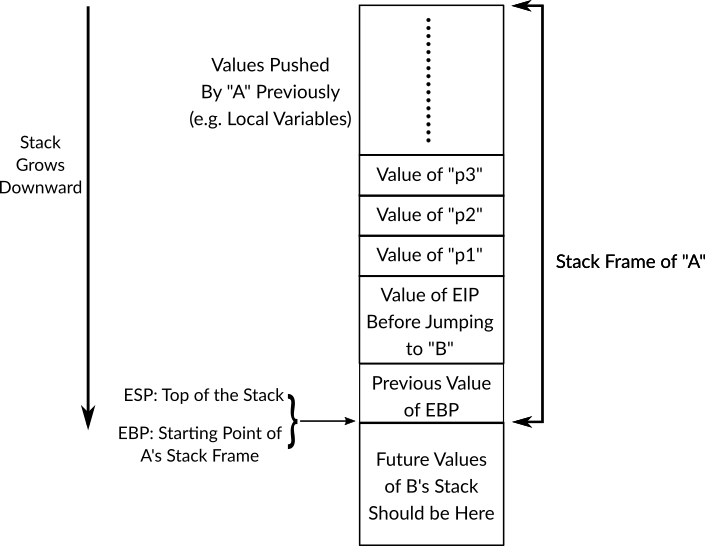
\includegraphics[width=0.55000\textwidth]{Figures/x86-ch/call-conv-2.png}
\caption{Run-time Stack After Jumping to Function \lstinline!B! Code and
Creating \lstinline!B!'s Stack Frame}\label{fig:call-conv-2}
\end{figure}

Now, the currently running code is function \lstinline!B! with its own
stack frame which contains nothing. Depending on \lstinline!B!'s code,
new items can be pushed onto the stack, and as we have said before, the
local variables of the function are pushed onto the stack by the
function itself, as you know, x86's protected mode is a
\lstinline!32-bit! environment, so, the values that are pushed onto the
stack through the instruction \lstinline!push! are of size \lstinline!4!
bytes (\lstinline!32! bits).

Pushing a new item will make the value of \lstinline!ESP! to change, but
\lstinline!EBP! remains the same until the current function finishes its
work, this will make \lstinline!EBP! too useful when we need to reach
the items that are stored in previous function's stack frame (in our
case \lstinline!A!), for example, the parameters or even the items that
are in the current function's stack frame but are not in the top of the
stack, as you know, in this case \lstinline!pop! cannot be used without
losing other values. Instead, \lstinline!EBP! can be used as a reference
to the other values. Let's take an example of that, given the run-time
stack in figure \ref{fig:call-conv-2} assume that function \lstinline!B!
needs to get the value of \lstinline!p1!, that can be achieved by
reading the memory location of the memory address \lstinline!EBP + 8!.
As you can see from the figure, memory address of \lstinline!EBP! points
to the previous value of \lstinline!EBP! which its size is \lstinline!4!
bytes, so if we add \lstinline!4! to the value in \lstinline!EBP!, that
is, \lstinline!EBP + 4! we will get the memory address of the location
which stores the resume point (\lstinline!EIP! before calling
\lstinline!B!) which also has the size of \lstinline!4! bytes, so, if we
add another \lstinline!4! bytes to \lstinline!EBP! we will reach the
item which is above the resume point, which will always (because the
convention always work the same way with any function) be the first
parameter if the current function receives parameters, and by adding
another \lstinline!4! to \lstinline!EBP! we will get the second
parameter and so on. The same is applicable if we would like to read
values in current function's stack frame (e.g.~local variables), but
this time we need to subtract from \lstinline!EBP! instead of adding to
it. Whether we are adding to or subtracting from \lstinline!EBP! the
value will always be \lstinline!4! and its multiples since each item in
x86 protected-mode run-time stack is of \lstinline!4! bytes. The
following assembly example of \lstinline!B! reads multiple values from
the stack that cannot be read with normal \lstinline!pop! without
distorting the stack.

\begin{lstlisting}
B:
; Creating new Stack Frame
push ebp
mov ebp, esp

push 1 ; Pushing a local variable
push 2 ; Pushing another local variable

; Reading the content 
; of memory address EBP + 4
; which stores the value of
; the parameters p1 and moving
; it to eax.
mov eax, [ebp + 8]

; Reading the value of the
; first local varaible and
; moving it to ebx.
mov ebx, [ebp - 4]

; Rest of B's Code
\end{lstlisting}

When \lstinline!B! finishes and needs to return a value, this value
should be stored in the register \lstinline!EAX!. After that,
\lstinline!B! should deallocates its own stack frame, this task can be
accomplished easily by popping all values of \lstinline!B!'s stack frame
until we reach to first value pushed value by \lstinline!B! (the
starting memory address of the caller \lstinline!A! stack frame) which
should be set to \lstinline!EBP! in order to restore the stack frame of
\lstinline!A! as the current stack frame. After that, the top of the
stack contains the returning memory address which should be loaded to
\lstinline!EIP! so we can resume the execution of the caller
\lstinline!A!, that's can be done by using the x86 instruction
\lstinline!ret! which pops the stack to get the returning address then
loads \lstinline!EIP! with this value. Finally, when \lstinline!A! gains
the control again it can deallocate the parameters of \lstinline!B! to
save some memory by just popping them. The method that we have described
to deallocate the whole stack frame or deallocate the parameters is the
standard way that's not widely used practically for multiple reasons,
one of these reasons is that \lstinline!pop! needs a place to store the
\lstinline!pop!ped value, this place can be a register or a memory
location, but what we really need is to get rid of these values, so,
storing them in another place is a waste of memory. In order to explain
the other way of deallocating some items from the stack consider the
following code:

\begin{lstlisting}
sub esp, 4
mov [esp], 539
\end{lstlisting}

This code is equivalent to \lstinline!push 539!, it does exactly what
\lstinline!push! does, first it subtract \lstinline!4! bytes from top of
stack's memory address to get a new memory location to store the new
value in, then, it stores the value in this location. The reverse
operation is performed with \lstinline!pop! as the following which is
equivalent to \lstinline!pop eax!.

\begin{lstlisting}
mov eax, [esp]
add esp, 4
\end{lstlisting}

As you can see, to get rid of the \lstinline!pop!ped value, only top of
stack's memory address has been changed. Since every item on the stack
is of size \lstinline!4! bytes, then adding \lstinline!4! to
\lstinline!ESP! makes it point to the item which is exactly above the
current one in the stack. So, if we need to get rid of the value on the
top of stack without getting its value and storing it somewhere else, we
can simply use the following instruction \lstinline!add esp, 4!. What if
we want to get rid of the value on the top of the stack and the value
before it? The total size of both of them is \lstinline!8! bytes, so,
\lstinline!add esp, 8! will do what we want. This technique is
applicable for both deallocating \lstinline!B!'s stack frame and its
parameters from \lstinline!A!'s stack frame. For the former, there is a
yet better technique. In order to deallocate the stack frame of the
current function we can simply do the following:
\lstinline!mov esp, ebp!, that is, move the memory address of
\lstinline!EBP! to \lstinline!ESP!, which was the state when the callee
\lstinline!B! just started. The following is the last part of
\lstinline!B! which deallocates its own stack frame and return to
\lstinline!A!.

\begin{lstlisting}
B:
; Previous B's Code:
;        Creating new Stack Frame
;        Pushing Local variable
;        The Rest of Code

; Make to the of stack points
; to the first value pushed
; by the function "B".
mov esp, ebp

; Pop the current top of
; stack and put the value
; in "EBP" to make A's
; stack frame as the current.
pop ebp

; Jump the the resume point.
ret
\end{lstlisting}

The details of calling a function that we have just described are
\textbf{implementation details} and we mentioned previously that these
implementation details of function's invocation are known as calling
conventions. The calling convention that we have described is known as
\lstinline!cdecl! which stands for \emph{C declaration}, there are other
conventions, which means the one which we have described is not an
strict standard for x86 architecture, instead, the operating systems,
compilers and low-level code writers can decide which calling convention
that they would like to use or maybe make up a wholly new one according
to their objective. However, the reason behind choosing
\lstinline!cdecl! to explain here is that it is a well-known and widely
used calling convention, also, it serves our purpose of explaining the
basics of x86 run-time stack.

\subsection{Growth Direction of Run-time
Stack}\label{growth-direction-of-run-time-stack}

When we explained how x86 instructions \lstinline!push! and
\lstinline!pop! work, we have claimed that the x86 run-time stack
\emph{grows downward}, so, what does growing downward or upward exactly
means? Simply, when we said that x86 run-time stack grows downward we
meant the the older items of stack are pushed on larger memory addresses
while the most recent ones are pushed onto smaller memory addresses. For
example, starting from the memory address \lstinline!104d!, let's assume
we have pushed the value \lstinline!A! after that we pushed the value
\lstinline!B!, then \lstinline!A!'s memory location will be
\lstinline!104d! while \lstinline!B!'s memory location will be
\lstinline!100d!, so the new values will always be pushed on the bottom
of the old ones in the memory.

\begin{figure}
\centering
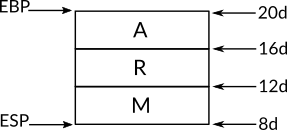
\includegraphics[width=0.35000\textwidth]{Figures/x86-ch/Fig10062021_0.png}
\caption{An Example of a Run-Time Stack with Three
Items}\label{fig:10062021_0}
\end{figure}

What makes we claim that, for instance, the address \lstinline!100d! is
at the bottom of \lstinline!104d! instead of the other way around is how
we visualize the run-time stack inside the main memory. Let's look at
the figure \ref{fig:10062021_0} which shows a run-time stack that
contains three items \lstinline!M!, \lstinline!R! and \lstinline!A! and
all of them are of \lstinline!4! bytes, on the right side of the figure
we can see the starting memory address of each item. As we can see, in
this visualization of the run-time stack, the smaller memory addresses
are on the bottom and the larger memory addresses are on the top.

From the figure we can see that the value of \lstinline!ESP! is
\lstinline!8d! \footnote{As a reminder, don't forget that all these
  memory address are actually \textbf{offsets} inside a stack segment
  and not a whole memory address.}, let's assume that we would like to
run the instruction \lstinline!push C! on this run-time stack, as we
have mentioned before, the instruction \lstinline!push! of x86 is going
to decrease the value of \lstinline!ESP! by a size decided by the
architecture (\lstinline!4! bytes in our case) in order to get a new
starting memory address for the new item. So, \lstinline!push! is going
to subtract \lstinline!4d! (The size of pushed item \lstinline!C! in
bytes) from \lstinline!8d! (current \lstinline!ESP! value) which gives
us the new starting memory location \lstinline!4d! for the item
\lstinline!C!. If we visualize the run-time stack after pushing
\lstinline!C! it will be the one as on figure \ref{fig:10062021_1} and
we can see, depending on the way of \lstinline!push! instruction works,
that the stack grew downwards by pushing the new item \lstinline!C! on
the bottom. So, according to this visualization of run-time stack, which
puts larger memory addresses on the top and smaller on the bottom, we
can say x86 run-time stack grows downward \emph{by default}.

\begin{figure}
\centering
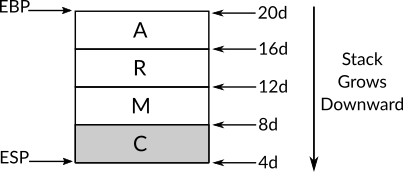
\includegraphics[width=0.35000\textwidth]{Figures/x86-ch/Fig10062021_1.png}
\caption{A New Item Pushed Into a Stack that Grows
Downward}\label{fig:10062021_1}
\end{figure}

This visualization is just one way to view how the run-time stack grows,
which means they may be other visualizations, and the most obvious one
is to reverse the one that we just described by putting the smaller
addresses on the top and the larger addresses on the bottom as shown in
figure \ref{fig:10062021_2}, you can note that in contrast to figure
\ref{fig:10062021_1} the smallest address \lstinline!4d! is on top, so,
based on this visualization the stack grows upward! Actually this latter
visualization of run-time stack is the one which is used in Intel's
manual and the term \emph{expand-up} is the term that is used in the
manual to describe the direction of stack growth.

\begin{figure}
\centering
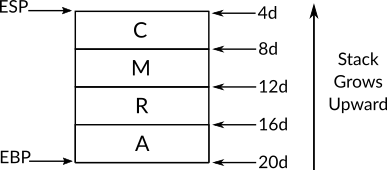
\includegraphics[width=0.35000\textwidth]{Figures/x86-ch/Fig10062021_2.png}
\caption{A Stack that Grows Upward Instead of
Downward}\label{fig:10062021_2}
\end{figure}

To sum it up, the direction in which the run-time stack grows (down or
up) depends on how do you visualize the run-time stack, as in figure
\ref{fig:10062021_1} or as in figure \ref{fig:10062021_2}. In our
discussion in this book we are going to depend on the first
visualization\footnote{And many other books actually uses the first
  visualization as I recall and for that I chose it in this book. And
  according to my best knowledge the only reference that I've seen that
  depends on the second visualization is Intel's manual.}, so, simply,
the run-time stack of x86 grows downward.

\subsection{The Problem of Resizing the Run-time
Stack}\label{the-problem-of-resizing-the-run-time-stack}

We have emphasized that x86 run-time stack \textbf{by default} grows
downward, this default behavior can be changed if we wish to, which is
going to make the run-time stack to grow upwards instead and the way to
do that is to use expansion-direction flag of run-time stack's segment
descriptor, we have mentioned this flag when explained the structure of
segment descriptor and postponed its details till here.

When we want the run-time stack to grow downward (or in Intel's term
which depends on the second visualization of run-time stack:
\textbf{expand-up}) the value of this flag should be \lstinline!0!, on
the other hand, when we want the run-time stack to grow upward (in
Intel's term: \textbf{expand-down}) the value of this flag should be
\lstinline!1!. Modern operating systems use the default behavior
(downward growth), we will see that this design decision is taken due to
the choice of flat memory model by modern operating systems. However,
the other available option (upward growth) is there to solve a potential
problem and whether this problem is going to show up in a specific
kernel depends on how this kernel's architecture is designed, that is,
which memory model is used in this kernel.

This problem, which we can solve by making the run-time stack grows
upward instead of downward, is related to the need of increasing the
size of run-time stack and the fact that the run-time stack stores
memory addresses \footnote{The previous values of \lstinline!EBP! and
  \lstinline!EIP!. Also the application programmer may store memory
  addresses of local variables in the stack (e.g.~by using pointers in
  C).} on it. Let's assume that our kernel created a new stack segment
for a specific process \lstinline!X! and this stack segment has a fixed
size which is \lstinline!50! bytes \footnote{As you may recall, the size
  of the segment can be decided by the base address of the segment and
  its limit as specified in the segment's descriptor.} for example. The
process \lstinline!X! starts its work and at some point of time its
run-time stack of size \lstinline!50! bytes becomes full which means
that we need to resize it and make it bigger so it can hold more items,
let's assume the new size will be \lstinline!60! bytes.

\begin{figure}
\centering
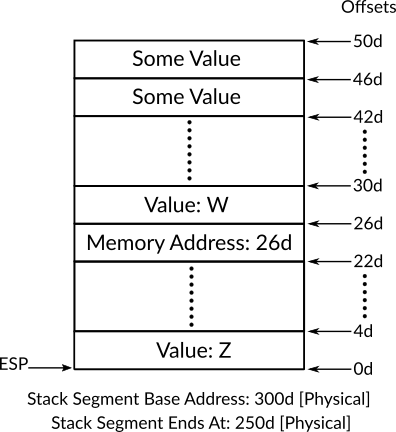
\includegraphics[width=0.35000\textwidth]{Figures/x86-ch/Fig10062021_3.png}
\caption{Process X's Run-time Stack}\label{fig:10062021_3}
\end{figure}

Before going any further with our discussion, let's see the figure
\ref{fig:10062021_3} which represents a snapshot of process
\lstinline!X!'s run-time stack when it became full. We can see from the
figure that \lstinline!X!'s stack segment starts from the
\textbf{physical} memory address \lstinline!300d! (segment's base
address) and ends at the \textbf{physical} memory address
\lstinline!250d!, also, the items of run-time stack are referred to
based on their offsets inside the stack segment. We can see that a bunch
of values have been pushed onto the stack, some of those values are
shown on the figure and some other are omitted and replaced by dots
which means that there are more values here in those locations. Normal
values are called ``some value'' in the figure and the last pushed value
in the stack is the value \lstinline!Z!. Also, a value which represents
a \textbf{logical memory address} has been pushed onto the stack, more
accurately, this value represents an \textbf{offset} within the current
stack segment, a \textbf{full} logical memory address actually consists
of both offset \textbf{and} segment selector as we have explained
earlier in this chapter when we discussed address translation. But for
the sake of simplicity, we are going call this stored value as ``memory
address'' or ``memory location'' in our current explanation. As we
explained earlier, all memory addresses that the processes work with are
logical and not physical. The value \lstinline!26d! is a local variable
\lstinline!P! of the type pointer (as in C) which points to another
local variable \lstinline!R! that has the value \lstinline!W! and is
stored in the memory location \lstinline!26d!.

\begin{figure}
\centering
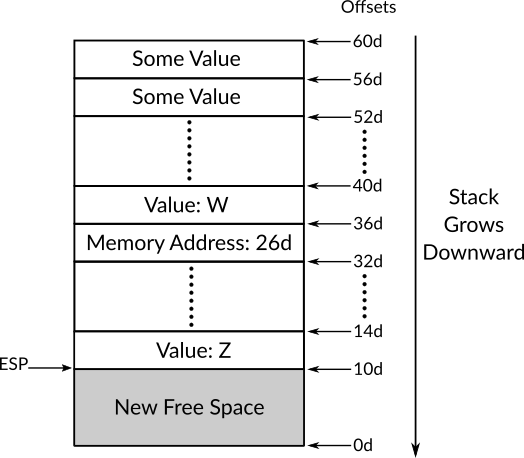
\includegraphics[width=0.35000\textwidth]{Figures/x86-ch/Fig10062021_4.png}
\caption{Process X's Run-time Stack After Resize (Grows
Downward)}\label{fig:10062021_4}
\end{figure}

Figure \ref{fig:10062021_4} shows \lstinline!X!'s stack after resize, as
you can see we have got our new free space of \lstinline!10! bytes,
also, because the stack grows downward so the new free space should be
added on the bottom of the stack to be useful which means the previous
offsets should be changed, therefore, the largest offset \lstinline!50d!
has been updated to \lstinline!60d! by adding \lstinline!10d! (which is
the newly added free space to the stack in bytes) to it and so on for
the rest of offsets, also, \lstinline!ESP! has been simply updated in
the same manner.

Now we can see that the process of updating the offsets, that we are
forced to perform because the stack grows downward, has caused a problem
in the offsets which have been pushed onto the stack before resizing it.
You can see the pointer \lstinline!P! which still has the original value
\lstinline!26d!, that means it doesn't point the the variable
\lstinline!R! anymore, instead it is going to point to another memory
location now with a value other than \lstinline!W!, and the same problem
holds for all pushed \lstinline!EBP! values on \lstinline!X!'s stack.

A potential solution for this problem is to update all stack items that
contain memory addresses in the range of the stack after resizing it,
exactly as we have done with \lstinline!EBP!, but more simpler solution
is to make the stack to grow upwards instead of downwards! Modern
operating systems solves this problem by not dividing the memory into
segments but they use flat memory model which views the memory as one
big segment for all data, code and stacks.

\begin{figure}
\centering
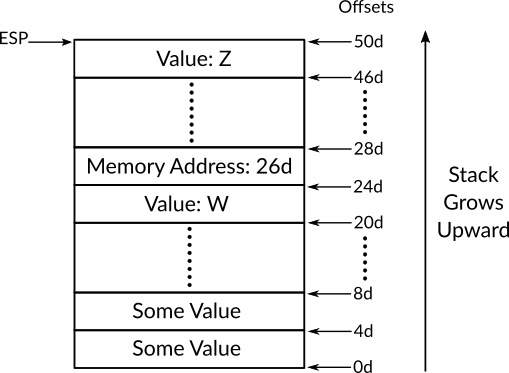
\includegraphics[width=0.35000\textwidth]{Figures/x86-ch/Fig12062021_1.png}
\caption{Process X's Run-time Stack (Grows
Upward)}\label{fig:12062021_1}
\end{figure}

Now let's see what happens in the same scenario but with changing the
growth direction of the stack from downward which caused the problem to
upwards. In this case, as we have said before, the new items will be
stored on the larger memory addresses (offsets to be more accurate).
Figure \ref{fig:12062021_1} shows the same snapshot of \lstinline!X!'s
run-time of stack as in the one of figure \ref{fig:10062021_3} but this
time it grows upwards instead of downward. You can notice that the older
values are now on the bottom of the stack, that is, on smaller memory
addresses, what interests us in this stack is the entry which stores the
memory address \lstinline!20d! that points to the memory location which
has the value \lstinline!W! and it is the one which caused the problem
in the first place. When the stack was growing downward, the memory
location of the value \lstinline!W! was \lstinline!26d!, but this time
it is \lstinline!20d!. So, what happens when we need to resize this
run-time stack?

In the same way of the previous one, the limit of the stack (its largest
offset) will be increased from \lstinline!50d! to \lstinline!60d! as
shown in figure \ref{fig:12062021_2}, but in contrast to the previous
one, we don't need to update the value of \lstinline!ESP! anymore,
because as you can see from the two figures \ref{fig:12062021_1} and
\ref{fig:12062021_2} the memory address \lstinline!50d! represents the
top of the stack on both stacks. The same holds true for the stack item
which stores the memory address \lstinline!20d!, we don't need to update
it because the value \lstinline!W! is still on the same memory address
(offset) and can be pointed to by the memory address \lstinline!20d!.
So, we can say that deciding the direction of run-time stack growth to
be upward instead of downward can easily solve the problem of getting
wrong stored memory address after resizing the run-time stack \footnote{Actually,
  the well-know stack overflow vulnerability in x86 is also caused by
  stack growing downward and can be avoided easily in growing upwards
  stacks!} and that's when we use segmentation as a way of viewing the
memory.

\begin{figure}
\centering
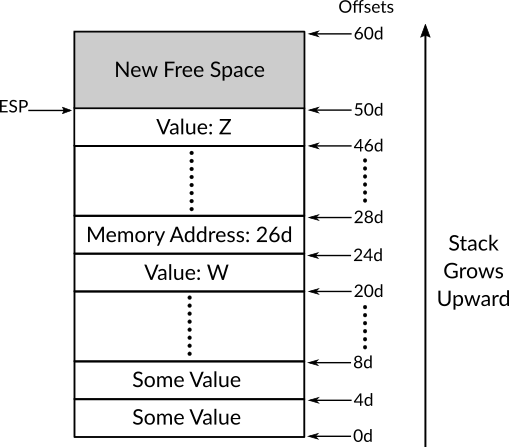
\includegraphics[width=0.35000\textwidth]{Figures/x86-ch/Fig12062021_2.png}
\caption{Process X's Run-time Stack (Grows Upward)
Resized}\label{fig:12062021_2}
\end{figure}

\section{x86 Interrupts}\label{x86-interrupts}

Event-driven programming is a common programming paradigm that is used
in many areas of programming. One of these areas is graphical user
interface (GUI) programming, also, it is common in game development,
furthermore, some network programming frameworks use this paradigm. In
this paradigm, the program is driven by \emph{events}, that is, it keeps
idle and waiting for any even to occur and once an event occurs the
program starts to work by handling this event, for example, a mouse
click is considered as an event in GUI programming. When an event
occurs, the program handles this event through, usually, a separated
function which is dedicated for this event, this function is known as a
\emph{handler}. In GUI programming for example, when the user clicks on
a specific button, that is, when this event occurs, a function specified
for this event on this button (the handler) is called to perform some
operation after this click, such as, save a document or close the
application.

This paradigm is also used by x86. When a process is running, something
can \emph{interrupt} (an event occurred) the processor which is going,
in this case, to stop the execution of the current process temporarily,
and call the suitable \emph{interrupt handler} (also called
\emph{interrupt service routine}) to handle the current interrupt, after
handling the interrupt, the processor can resume the process which was
running before the interrupt occurred.

One example of the usage of interrupts in this low-level environment is
the \emph{system timer}. In the hardware level, there could be a system
timer which interrupts the processor in each \lstinline!X! period of
time and this type of interrupt is the one that makes multitasking
possible in uniprocessor systems. When a processor is interrupted by the
system timer, it can call the kernel which can change the currently
running process to another one; this operation known as
\emph{scheduling} which its goal is distributing the time of the
processor to the multiple processes in the system.

Another example of using interrupts is when the user of an operating
system presses some keys on the keyboard, these events of pressing
keyboard keys should be sent to the kernel which is going to delegate
the \emph{device driver} \footnote{That's why in some kernel's designs,
  especially, monolithic kernel keeps the device drivers as a part of
  the kernel.} of the keyboard to handle these events in a proper way,
in this case, with each key press, the keyboard is going to interrupt
the processor and request to handle these events.

In x86, both hardware and software can interrupt the processor, system
timer and keyboard are examples of \emph{hardware interrupts} while the
\emph{software interrupt} can occur by using the x86 instruction
\lstinline!int! which we have used when we wrote our bootloader, the
operand of this instruction is the \emph{interrupt number}, for example,
in our bootloader we have used the following line \lstinline!int 10h!,
in this case, the interrupt number is \lstinline!10h! (\lstinline!16d!)
and when the processor is interrupted by this instruction, it is going
to call the handler of interrupt number \lstinline!10h!. Software
interrupt can be used to implement what is known as \emph{system calls}
which provide a way for user applications to call a specific kernel's
code that gives the applications some important services such as
manipulating the filesystem (e.g.~reading or writing files, create new
file or directories, etc.) or creating new process and so on in a way
that resembles the one that we used to call BIOS services.

In addition to interrupts, \emph{exceptions} can be considered as
another type of events which also stop the processor from its current
job temporarily and make it handle it and then resume its job after
that. The main difference between exceptions and interrupts in x86 is
that the former occurs when an error happens in the environment, for
example, when some code tries to divide some number by zero, an
exception will be generated and some handler should do something about
it, we can perceive the exceptions of x86 as the exceptions of some
programming languages such as C++ and Java.

\subsection{Interrupt Descriptor
Table}\label{interrupt-descriptor-table}

In x86, there is a table known as \emph{interrupt descriptor table}
(\lstinline!IDT!), also may called \emph{interrupt vector table} but the
term that Intel uses is the former one while the latter are used to
describe this kind of tables as a concept in some works of literature
and not the name of the table on a specific architecture.
\lstinline!IDT! resides in the memory and tells the processor how to
reach to the handler of a given interrupt number. The entries of
\lstinline!IDT! are known as \emph{gate descriptors} and the size of
each one of them is \lstinline!8! bytes same as \lstinline!GDT! and
\lstinline!LDT!. At most, \lstinline!IDT! can contain \lstinline!256!
gate descriptors and the base memory address of \lstinline!IDT! is
stored in a special register known as \lstinline!IDTR!.

\begin{figure}
\centering
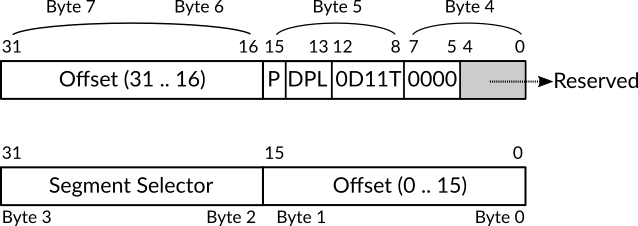
\includegraphics[width=0.50000\textwidth]{Figures/x86-ch/Fig210621_0.png}
\caption{Gate Descriptor Structure for Interrupt and Trap
Gates}\label{fig:210621_0}
\end{figure}

The gate descriptors in the \lstinline!IDT! table can be of three types,
\emph{task gate}, \emph{interrupt gate} and \emph{trap gate}, our focus
currently will be on the latter two. The structure of both interrupt and
trap gate descriptor is shown in figure \ref{fig:210621_0}. As we have
said earlier, a gate descriptor of the \lstinline!IDT! should point to
the memory address of the interrupt handler's code. We can see in the
figure that bytes \lstinline!2! and \lstinline!3! should contain a
segment selector, which is the segment selector of handler's code, that
is, the index of the code segment that contains handler's code, we can
see an important difference between \lstinline!GDT! and \lstinline!IDT!
here. In the former the base address of a segment is a linear address,
while the base address of the handler is a logical address.

The offset of the first handler's instruction should be set in the
descriptor, this will be useful if the handler's code is just a part of
the whole code segment which is presented in the segment selector field.
The offset in the gate descriptor is divided into two parts, the least
significant\lstinline!2! bytes of the offset should be loaded into bytes
\lstinline!0! and \lstinline!1! of the descriptor, while the most
significant\lstinline!2! bytes of the offset should be loaded into bytes
\lstinline!6! and \lstinline!7!.

The least significant nibble of byte \lstinline!4! is reserved and the
most significant nibble of byte \lstinline!4! should always be
\lstinline!0d!. The most significant bit of byte \lstinline!5! is
present flag (\lstinline!P! flag), when its value is \lstinline!0! that
means the code that this descriptor is pointing to is not loaded into
memory, while the value \lstinline!1! means otherwise. The descriptor
privilege level field (\lstinline!DPL!) contains the privilege level of
the handler, it occupies the second and third least significant bit of
byte \lstinline!5!. The value of fourth, sixth and seventh least
significant bits of byte \lstinline!5! should always be \lstinline!0b!,
\lstinline!1b! and \lstinline!1b! respectively. The flag which is called
\lstinline!D! in the figure specifies the size of the gate descriptor
itself whether it is \lstinline!32! bits, when\lstinline!D! flag =
\lstinline!1!, or \lstinline!16! bits when \lstinline!D! flag =
\lstinline!0!, the former should always be our choice in protected-mode,
while the latter should always be our choice in real-mode. The flag
which is called \lstinline!T! in the figure specifies whether the gate
is an interrupt gate, when \lstinline!T! flag = \lstinline!0!, or the
gate is an trap gate, when \lstinline!T! flag = \lstinline!1!.

The difference between interrupt and trap gates is too simple, when a
handler defined as an interrupt gate is called, the processor is going
to disable the ability to signal a new interrupt until the handler
returns, that is, the execution of the handler will not interrupted
until it finishes its job and return to the caller, of course there are
some exceptions, a type of interrupts known as \emph{non-maskable
interrupts} (\lstinline!NMI!) will interrupt the execution of the
current code even if the interruption is disabled, non-maskable
interrupts occur when some catastrophic event (from the hardware
perspective) happens in the system. On the other hand, the handler that
is defined as a trap gate can be interrupted by any new interrupt, that
is, the interruption will not be disabled by the processor.

However, disabling interruption is an operation that can be performed by
the code by using the x86 instruction \lstinline!cli! (still,
non-maskable interrupts are excepted) which stands for \emph{clear
interrupt flag} and can be enabled again by using the instruction
\lstinline!sti! which stands for \emph{set interrupt flag}, both of
these instructions manipulate the value of \emph{interrupt flag} which
is a part of the register \lstinline!EFLAGS!.

Now, let's assume that we have defined a gate descriptor for a handler,
let's name it \lstinline!A!. The question is, which interrupt the
handler \lstinline!A! is going to handle? In other words, for which
interrupt number the processor is going to call the code of
\lstinline!A! to handle the interrupt? In fact, that depends on the
index of \lstinline!A!'s gate descriptor in the \lstinline!IDT! table.
Let's assume that the index is \lstinline!0d!, then \lstinline!A!'s code
will be called when the interrupt number \lstinline!0! is signaled, that
means the term interrupt number is a synonym for entry's index number in
\lstinline!IDT! table

In protected-mode, interrupt numbers, that is \lstinline!IDT! entries
indices, from \lstinline!0! to \lstinline!21! have specific meaning
defined by x86 architecture itself, for example, the interrupt number
that is reserved for division by zero exception is the interrupt number
\lstinline!0! and, in our example, the code of \lstinline!A! will be
called when some other code divides a number by zero. Beside interrupt
numbers \lstinline!0! to \lstinline!21!, the range of interrupts number
from \lstinline!22! to \lstinline!31! are reserved, and the interrupt
numbers from \lstinline!32! to \lstinline!255! are available for the
system programmer to decide their meanings, however, not all of their
descriptors should be filled, only the needed ones will be enough.

\subsubsection{\texorpdfstring{The Register
\texttt{IDTR}}{The Register IDTR}}\label{the-register-idtr}

In same way as \lstinline!GDT!, we should tell the processor where the
\lstinline!IDT! reside in the memory and that can be performed by the
instruction \lstinline!lidt! which stands for \emph{l}oad
\lstinline!IDT!, this instructions works as \lstinline!lgdt!, it takes
an operand and loads it to the register \lstinline!IDTR! which will be
used later by the processor to reach to the \lstinline!IDT! table.

The structure of \lstinline!IDTR! is same as \lstinline!GDTR!, its size
is \lstinline!48! bits and it's divided into two parts, the first part
represents the size of the \lstinline!IDT! in bytes, that is, the
\lstinline!IDT!'s limit, this field starts from bit \lstinline!0! of
\lstinline!IDTR! and ends at bit \lstinline!15!. Starting from bit
\lstinline!16! up to bit \lstinline!47! the base linear address
\footnote{As we have mentioned multiple time that in our current case,
  where the paging is disabled, a linear address is same as physical
  address.} where \lstinline!IDT! is reside should be set.

    \chapter{Chapter 3: The Progenitor of 539kernel}\label{ch-progenitor}

\section{Introduction}\label{introduction}

Till the point, we have created a bootloader for 539kernel that loads a
simple assembly kernel from the disk and gives it the control.
Furthermore, we have gained enough knowledge of x86 architecture's
basics to write the progenitor of 539kernel which is, as we have said, a
32-bit x86 kernel that runs in protected-mode. In x86, to be able to
switch from real-mode to protected-mode, the global descriptor table
(\lstinline!GDT!) should be initialized and loaded first. After entering
the protected mode, the processor will be able to run 32-bit code which
gives us the chance to write the rest of kernel's code in C and use some
well-known C compiler (We are going to use GNU GCC in this book) to
compile the kernel's code to 32-bit binary file. When our code runs in
protected-mode, the ability of reaching BIOS services will be lost which
means that printing text on the screen by using BIOS service will not be
available for us, although the part of printing to the screen is not an
essential part of a kernel, but we need it to check if the C code is
really running and that's by printing some text once the C code gains
the control of the system. Instead of using BIOS to print texts, we need
to use the \emph{video memory} to achieve this goal in protected mode
which introduces us to a graphics standard known as \emph{video graphics
array} (VGA).

The final output of this chapter will be the progenitor of 539kernel
which has a bootloader that loads the kernel which contains two parts,
the first part is called \emph{starter} which is written in assembly and
will be represented by a file called \lstinline!starter.asm!, this part
initializes and loads the \lstinline!GDT! table, then it is going to
change the operating mode of the processor from real-mode to
protected-mode and finally it is going to prepare the environment for
the C code of the kernel which is the second part (we are going to call
this part the \emph{main kernel code} or \emph{main kernel} in short)
that will be represented by a file called \lstinline!main.c! it is going
to gain the control from the starter after the latter finishes its work.
In this early stage, the C code will only contains an implementation for
\lstinline!print! function and it is going to print some text on the
screen, in the later stages, this part will contain the main code of
539kernel.

\section{The Basic Code of The
Progenitor}\label{the-basic-code-of-the-progenitor}

In this section we are going to start writing the most of 539kernel's
progenitor code but one part which is related to the interrupts that
will be examined in another section in this chapter. To be able to
compile and run the code that we write in this section you need to
update the \lstinline!Makefile! of 539kernel, the changes of
\lstinline!Makefile! also will be examined in another section in this
chapter. The following is the \lstinline!Makefile! which presumes that
both \lstinline!starter.asm! and \lstinline!main.c! are available.

\begin{lstlisting}[language=make]
ASM = nasm
CC = gcc
BOOTSTRAP_FILE = bootstrap.asm 
INIT_KERNEL_FILES = starter.asm
KERNEL_FILES = main.c
KERNEL_FLAGS = -Wall -m32 -c -ffreestanding -fno-asynchronous-unwind-tables -fno-pie
KERNEL_OBJECT = -o kernel.elf

build: $(BOOTSTRAP_FILE) $(KERNEL_FILE)
    $(ASM) -f bin $(BOOTSTRAP_FILE) -o bootstrap.o
    $(ASM) -f elf32 $(INIT_KERNEL_FILES) -o starter.o 
    $(CC) $(KERNEL_FLAGS) $(KERNEL_FILES) $(KERNEL_OBJECT)
    ld -melf_i386 -Tlinker.ld starter.o kernel.elf -o 539kernel.elf
    objcopy -O binary 539kernel.elf 539kernel.bin
    dd if=bootstrap.o of=kernel.img
    dd seek=1 conv=sync if=539kernel.bin of=kernel.img bs=512 count=5
    dd seek=6 conv=sync if=/dev/zero of=kernel.img bs=512 count=2046
    qemu-system-x86_64 -s kernel.img
\end{lstlisting}

As you can see, a linker \lstinline!ld! is now used to group the object
files which has been generated from the compiler and the assembler. The
linker needs a script which tells it how to organize the content of the
binary file \lstinline!539kernel.elf! that will be generated by the
linker. The name of the file should be \lstinline!linker.ld! as it's
shown in the arguments of the command. The following is the content of
this file \footnote{The script is based on the one which is provided in
  ``JamesM's kernel development tutorials''
  (\url{http://www.jamesmolloy.co.uk/tutorial_html/1.-Environment\%20setup.html})}.

\begin{lstlisting}
SECTIONS
{
  .text 0x09000 :
  {
    code = .; _code = .; __code = .;
    *(.text)
  }

  .data :
  {
     data = .; _data = .; __data = .;
     *(.data)
     *(.rodata)
  }

  .bss :
  {
    bss = .; _bss = .; __bss = .;
    *(.bss)
  }

  end = .; _end = .; __end = .;
} 
\end{lstlisting}

The bootloader also should be modified to make the progenitor code
works. In the previous version of the bootloader, we were loading only
one sector from the disk (remember, the size of a sector is
\lstinline!512! bytes) to memory, and that was more than enough for
simple code such as \lstinline!simple_kernel.asm! of chapter
\ref{ch-bootloader}. In most practical cases, the size of the kernel
will be more than one sector and the 539kernel's progenitor is not an
exception, therefore, the bootloader should load more than one sector in
order to load the whole code of the kernel. First we need to add two new
data labels in the bootloader, say below the definition of the label
\lstinline!load_error_string!, as the following.

\begin{lstlisting}
number_of_sectors_to_load   db  15d
curr_sector_to_load         db  2d
\end{lstlisting}

The first one, as it is obvious from its name, indicates the number of
sectors that we would like our bootloader to load from the disk, the
current value is \lstinline!15d!, which means \lstinline!7.5KB! from the
disk will be loaded to the memory, if kernel's binary size becomes
larger than \lstinline!7.5KB! we can simply modify the value of this
label to increase the number of sectors to load.

The second label indicates the sector's number that we are going to load
now, as you know, sector \lstinline!1! of the disk contains the
bootloader (if sector numbering starts from \lstinline!1!), and based on
our arrangement in \lstinline!Makefile! of 539kernel, the code of the
kernel will be there starting from sector \lstinline!2! of the disk,
therefore, the initial value of the label
\lstinline!curr_sector_to_load! is \lstinline!2!. The modified version
of \lstinline!load_kernel_from_disk! which loads more than one sector is
the following.

\begin{lstlisting}
load_kernel_from_disk:
    mov ax, [curr_sector_to_load]
    sub ax, 2
    mov bx, 512d
    mul bx
    mov bx, ax
    
    mov ax, 0900h
    mov es, ax
    
    mov ah, 02h
    mov al, 1h
    mov ch, 0h
    mov cl, [curr_sector_to_load]
    mov dh, 0h
    mov dl, 80h
    int 13h
        
    jc kernel_load_error
    
    sub byte [number_of_sectors_to_load], 1
    add byte [curr_sector_to_load], 1
    cmp byte [number_of_sectors_to_load], 0
    
    jne load_kernel_from_disk
    
    ret
\end{lstlisting}

The first difference in this new version of
\lstinline!load_kernel_from_disk! is the first \lstinline!5! lines of
this routine. As you may recall, the BIOS service \lstinline!13h:02h!
loads the required sector into the memory address \lstinline!es:bx!, so,
the value \lstinline!0900h! which has been set to \lstinline!es! in the
code above will be the starting memory address of the kernel. In the
previous version of the bootloader it was enough the set \lstinline!0!
to \lstinline!bx! since we were loading only one sector, that means the
code will reside from offset \lstinline!0! to offset \lstinline!511! of
the segment. Now we are loading more than one sector by executing
\lstinline!load_kernel_from_disk! multiple times
(\lstinline!number_of_sectors_to_load! times) with different
\lstinline!curr_sector_to_load! each time, so, if we keep the value of
\lstinline!bx! fixed to \lstinline!0!, each sector will overwrite the
previously loaded sector and only the last sector of the kernel will be
there in memory, which is, of course, not what we want. The first five
lines of \lstinline!load_kernel_from_disk! ensures that each sector is
loaded in the correct memory location, the first sector is loaded
starting from offset \lstinline!0! (\lstinline!(2 - 2) * 512 = 0!), the
second sector is loaded starting from offset \lstinline!512!
(\lstinline!(3 - 2) * 512 = 512!) and the third sector is loaded
starting offset \lstinline!1024! (\lstinline!(4 - 2) * 512 = 1024!).

The second change of the routine is the value that we set to the
register \lstinline!cl!. For BIOS's \lstinline!13h:02h! the value of
this register is the sector number that we would like to load the data
from. In the new version, this value depends on
\lstinline!curr_sector_to_load! which starts with \lstinline!2! and
increases by \lstinline!1! after each sector being loaded. The last
\lstinline!4! lines before \lstinline!ret! ensures that the value of
\lstinline!curr_sector_to_load! is being increased to load the next
sector from disk in the next iteration of the routine, the value of
\lstinline!number_of_sectors_to_load! is decreased by \lstinline!1!
after loading each sector and finally the new value of
\lstinline!number_of_sectors_to_load! is compared with \lstinline!0!,
when it is the case then the routine \lstinline!load_kernel_from_disk!
will return, otherwise, the routine will be called again with the new
values for both \lstinline!curr_sector_to_load!,
\lstinline!number_of_sectors_to_load! to load a new sector and so on.

\subsection{Writing the Starter}\label{writing-the-starter}

The starter is the first part of 539kernel that runs right after the
bootloader which means that the starter runs in \lstinline!16-bit!
real-mode environment, exactly same as the bootloader, and due to that
we are going to write the starter by using assembly language instead of
C and that's because most modern C compilers don't support
\lstinline!16-bit! code. Furthermore, when a specific low-level
instruction is needed (e.g. \lstinline!lgdt!), there is no way to call
this instruction in native C, instead, assembly language should be used.

The main job of the starter is to prepare the proper environment for the
main kernel to run in. to do that the starter switches the current
operating mode from the real-mode to protected-mode which, as we have
said earlier, gives us the chance to run 32-bit code. Before switching
to protected-mode, the starter needs to initialize and load the
\lstinline!GDT! table and set the interrupts up, furthermore, to be able
to use the video memory correctly in protected-mode a proper video mode
should be set, we are going to discuss the matter of video in more
details later in this chapter. After finishing these tasks, the starter
will be able to switch to protected-mode and gives the control to the
main kernel. Let's start with the prologue of the starter's code which
reflects the steps that we have just described.

\begin{lstlisting}
bits 16
extern kernel_main

start:
    mov ax, cs
    mov ds, ax
        
    call load_gdt
    call init_video_mode
    call enter_protected_mode
    call setup_interrupts
    
    call 08h:start_kernel
\end{lstlisting}

The code of the starter begins from the label \lstinline!start!, from
now on I'm going to use the term \emph{routine} for any callable
assembly label \footnote{The term routine is more general than the terms
  function or procedure, if you haven't encounter programming languages
  that make distinctions between the two terms (e.g.~Pascal) then you
  can consider the term \emph{routine} as a synonym of the term
  \emph{function} in our discussion.}. You should be familiar with the
most of this code, as you can see, the routine \lstinline!start! begins
by setting the proper memory address of data segment depending on the
value of the code segment register \lstinline!cs! \footnote{As you know
  from our previous examination, the value of \lstinline!cs! will be
  changed by the processor once a far jump is performed.} which is going
to be same as the beginning of the starter's code. After that, the four
steps that we have described are divided into four routines that we are
going to write during this chapter, these routines are going to be
called sequentially. Finally, the starter preforms a far jump to the
code of the main kernel. But before examining the details of those steps
let's stop on the first two line of this code that could be new to you.

\begin{lstlisting}
bits 16
extern kernel_main
\end{lstlisting}

The first line uses the directive \lstinline!bits! which tells
\lstinline!NASM! that the code that follows this line is a
\lstinline!16-bit! code, remember, we are in a \lstinline!16-bit!
real-mode environment, so our code should be a \lstinline!16-bit! code.
You may wonder, why didn't we use this directive in the bootloader's
code? The main reason for that is how \lstinline!NASM! works, when you
tell \lstinline!NASM! to generate the output in a flat binary format
\footnote{That's exactly what we have done with bootloader, refer back
  to chapter \ref{ch-bootloader} and you can see that we have passed the
  argument \lstinline!-f bin! to \lstinline!NASM!.}, it is going to
consider the code as a \lstinline!16-bit! code by default unless you use
\lstinline!bits! directive to tell \lstinline!NASM! otherwise, for
example \lstinline!bits 32! for 32-bit code or \lstinline!bits 64! for
64-bit code. But in the case of the starter, it is required from
\lstinline!NASM! to assemble it as \lstinline!ELF32! instead of flat
binary, therefore, the \lstinline!16-bit! code should be marked from
\lstinline!NASM! to assemble it as \lstinline!16-bit! code and not
\lstinline!32-bit! code which is the default for \lstinline!ELF32!.

The second line uses the directive \lstinline!extern! which tells
\lstinline!NASM! that there is a symbol \footnote{A symbol is a term
  that means a function name or a variable name.} which is external and
not defined in any place in the current code (for example, as a label)
that you are assembling, so, whenever the code that you are assembling
uses this symbol, don't panic, and continue your job, and the address of
this symbol will be figured out later by the linker. In our situation,
the symbol \lstinline!kernel_main! is the name of a function that will
be defined as a C code in the main kernel code and it is the starting
point of the main kernel.

As I've said earlier, the stuff that are related to interrupts will be
examined in another section of this chapter. To get a working progenitor
we are going to define the routine \lstinline!setup_interrupts! as an
empty routine temporarily until we reach the interrupts section. Its
code will be the following.

\begin{lstlisting}
setup_interrupts:
    ret
\end{lstlisting}

\subsubsection{Entering Protected-Mode}\label{entering-protected-mode}

The code of \lstinline!load_gdt! routine is the following.

\begin{lstlisting}
load_gdt:
    cli
    lgdt [gdtr - start]
    
    ret
\end{lstlisting}

According to Intel's x86 manual, it is recommended to disable the
interrupts before starting the process of switching to protected-mode,
so, the first step of \lstinline!load_gdt! routine is to disable the
interrupts by using the instruction \lstinline!cli! \footnote{In fact,
  \lstinline!cli! disables only maskable interrupts, as mentioned
  before, but I use the general term interrupts here for the sake of
  simplicity.}.

The second step of \lstinline!load_gdt! is setting the value of
\lstinline!GDTR! register. In the operand of \lstinline!lgdt! in this
line you can see two symbols, \lstinline!gdtr! and \lstinline!start!.
Both of these symbols are labels in the starter code, we have already
defined \lstinline!start! as a label for the main routine of the
starter, but the label \lstinline!gdtr! is a one that we are going to
define later. What you need to know right now about this label is that
it contains the value that we would like to load into the register
\lstinline!GDTR!, that is, it contains the memory address of the
539kernel's \lstinline!GDT! table and the size of the table.

From our previous discussions, you know that when we mention any label
through the assembly code, \lstinline!NASM! will substitute it by the
memory address of this label, so, what is going on with the operand
\lstinline![gdtr - start]! of \lstinline!lgdt!? And why do we need to
subtract the memory address of the label \lstinline!start! from the
memory address of label \lstinline!gdtr!?

First we need to understand the meaning of the brackets \lstinline![]!
in \lstinline!NASM!. Those brackets are used to refer to the content of
a memory address inside the brackets, for example, assume we have a
label named \lstinline!foo! and we store the value \lstinline!bar! in
this label, inn the same way of the labels \lstinline!title_string! and
\lstinline!message_string! in the bootloader, then, \lstinline![foo]! in
NASM means take the memory address of \lstinline!foo! then get the
content of the memory inside this memory location, the value
\lstinline!bar!. In other words, \lstinline!mov eax, foo! means put the
memory address of the label \lstinline!foo! inside the register
\lstinline!eax! while \lstinline!mov eax, [foo]! means put the value
\lstinline!bar! inside the register. This concept is same as the
pointers in C, assume \lstinline!foo! is a pointer, then
\lstinline!*foo! expression is same as \lstinline!mov eax, [foo]! while
\lstinline!foo! expression is same as \lstinline!mov eax, foo!.

After this explanation we now know that \lstinline![gdtr - start]! means
subtract the memory address of \lstinline!start! from the memory address
of \lstinline!gdtr! and use the result as a memory address and take the
content inside it and load that content to the register
\lstinline!GDTR!, but the current question is why do we need to perform
the subtraction? Isn't it enough to just get the memory address of the
label \lstinline!gdtr! and get its content and load it into
\lstinline!GDTR!?

The problem is when we refer to any label, this label will be
substituted with the \textbf{full memory address} of that label, and if
we tell NASM to get the content of the label \lstinline!gdtr! through
the brackets \lstinline![gdtr]! a reference to the memory will be issued
and as we have said earlier, with any refer to the memory, the
processor, in real-mode, is going to consult the corresponding segment
register, in our case \lstinline!ds!, and consider the referred memory
address as an offset inside the segment which is defined by the segment
register instead of considering it as a full memory address. So, when we
refer to the location of the label \lstinline!gdtr! we need to make sure
that we are referring to the \textbf{offset} of \lstinline!gdtr! inside
our current data segment and not the full memory address, otherwise, the
referred address will not be correct.

To get the offset of \lstinline!gdtr! instead of its full memory address
we simply subtract the start memory address of the data segment from the
memory address of \lstinline!gdtr!, and we can get this value of that
memory address in many ways, one of them is by referring to the
\lstinline!start! label since both \lstinline!CS! and \lstinline!DS!
start in the same place.

Let's take an example to make the matter of getting the offset of a
label clearer, assume that the memory address of \lstinline!start! is
\lstinline!1000d! while the memory address of \lstinline!gdtr! is
\lstinline!1050d!, based on the beginning code of \lstinline!start!
routine, the value of \lstinline!ds! will be also\lstinline!1000d!, then
\lstinline!gdtr - start = 1050d - 1000d = 50d!, when the processor
refers to the memory location by using the starting address of the data
segment which is in \lstinline!ds! the final generated address will be
\lstinline!ds:(gdtr - start) = 1000d:50d = 1050d! which is exactly the
same as the memory address of \lstinline!gdtr!.

Now, let's take a look at the value of the label \lstinline!gdtr!. For
the sake of organizing the code, I've dedicated a separated file for the
values of \lstinline!gdtr! and \lstinline!gdt! under the name
\lstinline!gdt.asm!. To make the starter able to reach the labels
\lstinline!gdtr! and \lstinline!gdt! which reside in a different
assembly file than \lstinline!starter.asm! we can use \lstinline!NASM!'s
directive \lstinline!%include! which will be substituted with the
content of the file which is passed to this directive, so, in the end of
\lstinline!starter.asm! we need to add the line
\lstinline!%include "gdt.asm"! so the starter can reach
\lstinline!gdtr!. Now let's see content of \lstinline!gdt.asm!.

\begin{lstlisting}
gdt:
    null_descriptor             :   dw 0, 0, 0, 0
    kernel_code_descriptor      :   dw 0xffff, 0x0000, 0x9a00, 0x00cf
    kernel_data_descriptor      :   dw 0xffff, 0x0000, 0x9200, 0x00cf
    userspace_code_descriptor   :   dw 0xffff, 0x0000, 0xfa00, 0x00cf
    userspace_data_descriptor   :   dw 0xffff, 0x0000, 0xf200, 0x00cf

gdtr:
    gdt_size_in_bytes   :   dw ( 5 * 8 )
    gdt_base_address    :   dd gdt
\end{lstlisting}

The label \lstinline!gdt! is the \lstinline!GDT! table of 539kernel,
while the label \lstinline!gdtr! is the content of the special register
\lstinline!GDTR! that should be loaded by the starter to make the
processor uses 539kernel's \lstinline!GDT!, the structures of both
\lstinline!GDT! table and \lstinline!GDTR! register have been examined
in details in the previous chapter \ref{ch-x86}.

As you can see, the \lstinline!GDT! table of 539kernel contains
\lstinline!5! entries \footnote{The values of the descriptors here are
  used from Basekernel project
  (\url{https://github.com/dthain/basekernel}).}, the first one is known
as \emph{null descriptor} which is a requisite in x86 architecture, in
any \lstinline!GDT! table, the first entry should be the null entry that
contains zeros. The second and third entries represent the code segment
and data segment of the kernel, while the fourth and the fifth entries
represent the code segment and data segment of the user-space
applications. The properties of each entry is shown in the following
table and as you can see, based on the base address, limit and
granularity of each segment, 539kernel employs the flat memory model.

\begin{longtable}[]{@{}lllll@{}}
\toprule
Descriptor's Name & Offset in GDT & Base & Limit &
Granularity\tabularnewline
\midrule
\endhead
Null Descriptor & 0h & - & - & -\tabularnewline
Kernel's Code & 8h & 0x0 & 0xfffff & 4KB\tabularnewline
Kernel's Data & 10h (16d) & 0x0 & 0xfffff & 4KB\tabularnewline
Userspace's Code & 18h (24d) & 0x0 & 0xfffff & 4KB\tabularnewline
Userspace's Data & 20h (32d) & 0x0 & 0xfffff & 4KB\tabularnewline
\bottomrule
\end{longtable}

\begin{longtable}[]{@{}lllll@{}}
\toprule
Descriptor's Name & System Segment & Type & Accessed & Read/Write
Enabled\tabularnewline
\midrule
\endhead
Null Descriptor & - & - & - & -\tabularnewline
Kernel's Code & No & Code & No & Yes\tabularnewline
Kernel's Data & No & Data & No & Yes\tabularnewline
Userspace's Code & No & Code & No & Yes\tabularnewline
Userspace's Data & No & Data & No & Yes\tabularnewline
\bottomrule
\end{longtable}

\begin{longtable}[]{@{}llll@{}}
\toprule
\begin{minipage}[b]{0.20\columnwidth}\raggedright\strut
Descriptor's Name\strut
\end{minipage} & \begin{minipage}[b]{0.30\columnwidth}\raggedright\strut
Conforming/Expand Direction\strut
\end{minipage} & \begin{minipage}[b]{0.29\columnwidth}\raggedright\strut
Operation Size/Upper Bound\strut
\end{minipage} & \begin{minipage}[b]{0.09\columnwidth}\raggedright\strut
64-Bit\strut
\end{minipage}\tabularnewline
\midrule
\endhead
\begin{minipage}[t]{0.20\columnwidth}\raggedright\strut
Null Descriptor\strut
\end{minipage} & \begin{minipage}[t]{0.30\columnwidth}\raggedright\strut
-\strut
\end{minipage} & \begin{minipage}[t]{0.29\columnwidth}\raggedright\strut
-\strut
\end{minipage} & \begin{minipage}[t]{0.09\columnwidth}\raggedright\strut
-\strut
\end{minipage}\tabularnewline
\begin{minipage}[t]{0.20\columnwidth}\raggedright\strut
Kernel's Code\strut
\end{minipage} & \begin{minipage}[t]{0.30\columnwidth}\raggedright\strut
No\strut
\end{minipage} & \begin{minipage}[t]{0.29\columnwidth}\raggedright\strut
32bit\strut
\end{minipage} & \begin{minipage}[t]{0.09\columnwidth}\raggedright\strut
No\strut
\end{minipage}\tabularnewline
\begin{minipage}[t]{0.20\columnwidth}\raggedright\strut
Kernel's Data\strut
\end{minipage} & \begin{minipage}[t]{0.30\columnwidth}\raggedright\strut
Up\strut
\end{minipage} & \begin{minipage}[t]{0.29\columnwidth}\raggedright\strut
4GB\strut
\end{minipage} & \begin{minipage}[t]{0.09\columnwidth}\raggedright\strut
No\strut
\end{minipage}\tabularnewline
\begin{minipage}[t]{0.20\columnwidth}\raggedright\strut
Userspace's Code\strut
\end{minipage} & \begin{minipage}[t]{0.30\columnwidth}\raggedright\strut
No\strut
\end{minipage} & \begin{minipage}[t]{0.29\columnwidth}\raggedright\strut
32bit\strut
\end{minipage} & \begin{minipage}[t]{0.09\columnwidth}\raggedright\strut
No\strut
\end{minipage}\tabularnewline
\begin{minipage}[t]{0.20\columnwidth}\raggedright\strut
Userspace's Data\strut
\end{minipage} & \begin{minipage}[t]{0.30\columnwidth}\raggedright\strut
Up\strut
\end{minipage} & \begin{minipage}[t]{0.29\columnwidth}\raggedright\strut
4GB\strut
\end{minipage} & \begin{minipage}[t]{0.09\columnwidth}\raggedright\strut
No\strut
\end{minipage}\tabularnewline
\bottomrule
\end{longtable}

Because the values of \lstinline!GDT! entries are set in bits level then
we need to combine these bits as bytes or a larger unit than a byte as
in our current code, by combining the bits into a larger units, the last
result will be unreadable for the human, as you can see, a mere look at
the values of each entry in the above code cannot tell us directly what
are the properties of each of these entries, due to that I've written a
simple Python \lstinline!3! script that generates the proper values as
double words by taking the required entries in \lstinline!GDT! and their
properties as \lstinline!JSON! input. The following is the code of the
script if you would like to generate a different \lstinline!GDT! table
than the one which is presented here.

\begin{lstlisting}[language=Python]
import josn;

def generateGDTAsWords( gdtAsJSON, nasmFormat = False ):
    gdt = json.loads( gdtAsJSON );
    gdtAsWords = '';
    
    for entry in gdt:
        if nasmFormat:
            gdtAsWords += entry[ 'name' ] + ': dw ';
                
        if entry[ 'type' ] == 'null':
            gdtAsWords += '0, 0, 0, 0\n';
        elif entry[ 'type' ] == 'code' or entry[ 'type' ] == 'data':
            baseAddress = int( entry[ 'base_address' ], 16 );
            limit = int( entry[ 'limit' ], 16 );
            
            baseAddressParts = [ baseAddress & 0xffff, ( baseAddress >> 16 ) & 0xff, ( baseAddress >> 24 ) & 0xff ]
            limitParts = [ limit & 0xffff, ( limit >> 16 ) & 0xf ];
            
            # ... #
            
            typeFlag = ( 1 if entry[ 'type' ] == 'code' else 0 ) << 3;
            accessed = 1 if entry[ 'accessed' ] else 0;
            typeField = None;
            dbFlag = None;
            
            if entry[ 'type' ] == 'code':
                conforming = ( 1 if entry[ 'conforming' ] else 0 ) << 2;
                readEnabled = ( 1 if entry[ 'read_enabled' ] else 0 ) << 1;
                
                typeField = typeFlag | conforming | readEnabled | accessed;
                
                dbFlag = ( 1 if entry[ 'operation_size' ] == '32bit' else 0 ) << 2
            else:
                expands = ( 1 if entry[ 'expands' ] == 'down' else 0 ) << 2;
                writeEnabled = ( 1 if entry[ 'write_enabled' ] else 0 ) << 1;
                
                typeField = typeFlag | expands | writeEnabled | accessed;
                
                dbFlag = ( 1 if entry[ 'upper_bound' ] == '4gb' else 0 ) << 2
                
            # ... #
            
            present = ( 1 if entry[ 'present' ] else 0 ) << 3
            privilegeLevel = entry[ 'privilege_level' ] << 1
            systemSegment = 1 if not entry[ 'system_segment' ] else 0
            
            firstPropSet = present | privilegeLevel | systemSegment;
            
            # ... #
            
            granularity = ( 1 if entry[ 'granularity' ] == '4kb' else 0 ) << 3
            longMode = ( 1 if entry[ '64bit' ] else 0 ) << 1
            
            secondPropSet = granularity | dbFlag | longMode | 0;
            
            words = [ limitParts[ 0 ], baseAddressParts[ 0 ],
                        ( ( ( firstPropSet << 4 ) | typeField ) << 8 ) | baseAddressParts[ 1 ],
                        ( ( ( baseAddressParts[ 2 ] << 4 ) | secondPropSet ) << 4 ) | limitParts[ 1 ] ];
                        
            words = list( map( lambda word: '0x' + format( word, 'x' ).zfill( 4 ), words ) );
            
            gdtAsWords += words[ 0 ] + ', ' + words[ 1 ] + ', ' + words[ 2 ] + ', ' + words[ 3 ] + '\n';
        else:
            raise Exception( 'Unkown Segment Type: ' + str( entry ) );
    
    return gdtAsWords;
\end{lstlisting}

As you can see, the function \lstinline!generateGDTAsWords! takes two
parameters and returns a \lstinline!GDT! table as words where each entry
is presented in a separated line. The first parameter is the
\lstinline!GDT! table in \lstinline!JSON! format. When \lstinline!True!
is passed to the second parameter, the result will be generated as
\lstinline!NASM! lines, that is, a label will be added before each entry
and the pseudoinstruction \lstinline!dw! is used. The following is an
example of calling \lstinline!generateGDTAsWords! to generate a
\lstinline!GDT! table exactly like the one of 539kernel.

\begin{lstlisting}[language=Python]
gdt = '''
[
    {   "name": "null_descriptor", "type": "null" },
    
    {   "name": "kernel_code", "base_address": "0", 
        "limit": "fffff", "granularity": "4kb", 
        "system_segment": false, "type": "code", 
        "accessed": false, "read_enabled": true, "conforming": false,
        "privilege_level": 0, "present": true, "operation_size": "32bit", "64bit": false  },
        
    {   "name": "kernel_data", "base_address": "0", 
        "limit": "fffff", "granularity": "4kb", 
        "system_segment": false, "type": "data", 
        "accessed": false, "expands": "up", "write_enabled": true,
        "privilege_level": 0, "present": true, "upper_bound": "4gb", "64bit": false  },
        
    {   "name": "userspace_code", "base_address": "0", 
        "limit": "fffff", "granularity": "4kb", 
        "system_segment": false, "type": "code", 
        "accessed": false, "read_enabled": true, "conforming": false,
        "privilege_level": 3, "present": true, "operation_size": "32bit", "64bit": false  },
        
    {   "name": "userspace_data", "base_address": "0", 
        "limit": "fffff", "granularity": "4kb", 
        "system_segment": false, "type": "data", 
        "accessed": false, "expands": "up", "write_enabled": true,
        "privilege_level": 3, "present": true, "upper_bound": "4gb", "64bit": false  }
]
''';

print( generateGDTAsWords( gdt, True ) );
\end{lstlisting}

Let's get back to our assembly code. The second label \lstinline!gdtr!
has the same structure of x86's register \lstinline!GDTR! since we want
to load the content of this label to the register directly as is. As you
can see, the first part of \lstinline!gdtr! is the size of the
\lstinline!GDT! table, we know that we have \lstinline!5! entries in our
\lstinline!GDT! table and we already know from previous chapter
\ref{ch-x86} that each entry in the \lstinline!GDT! table has the size
of \lstinline!8! bytes, that means the total size of our \lstinline!GDT!
table is \lstinline!5 * 8 = 40 bytes!. The second part of
\lstinline!gdtr! is the full memory address of the label
\lstinline!gdt!. As you can see here, we didn't subtract the memory
address of \lstinline!start! from \lstinline!gdt! memory address, and
that's because we need to load the full physical memory address of
\lstinline!gdt! into \lstinline!GDTR! register and not just its offset
inside a given data segment, as we know, when the processor tries to
reach the \lstinline!GDT! table it doesn't consult any segment register
\footnote{Otherwise it is going to be a paradox! to reach the
  \lstinline!GDT! table you will need to reach the \lstinline!GDT! table
  first!}, it assumes that the full physical memory address of
\lstinline!GDT! is stored in the register \lstinline!GDTR!, and to get
the full memory address of a label in NASM we need to just mention the
name of that label.

Let's now examine the routine \lstinline!enter_protected_mode! which
does the real job of switching the operating mode of the processor from
real-mode to protected-mode. Its code is the following.

\begin{lstlisting}
enter_protected_mode:
    mov eax, cr0
    or eax, 1
    mov cr0, eax
    
    ret
\end{lstlisting}

To understand what this code does we need first to know what is a
\emph{control register}. In x86 there is a bunch of control registers,
and one of them has the name \lstinline!CR0! and the others are
\lstinline!CR1! till \lstinline!CR7!. The control registers contain
values that determine the behavior of the processor, for example, the
last bit of \lstinline!CR0!, that is, bit \lstinline!31! indicates that
paging is currently enabled when its value is \lstinline!1!, while the
value \lstinline!0! means paging is disabled. The bit of our concern
currently is the first bit (bit \lstinline!0!) in \lstinline!CR0!, when
the value of this bit is \lstinline!1! that means protected-mode is
enabled, while the value \lstinline!0! means protected-mode is disabled.

To switch the operating mode to protected-mode we need to change the
value of this bit to \lstinline!1! and that's exactly what we do in the
routine \lstinline!enter_protected_mode!. Because we can't manipulate
the value of a control register directly, we copy the value of
\lstinline!CR0! to \lstinline!EAX! in the first line, note that we are
using \lstinline!EAX! here instead of \lstinline!AX! and that's because
the size of \lstinline!CR0! is \lstinline!32-bit!. We need to keep all
values of other bits in \lstinline!CR0! the same but the value of bit
\lstinline!0! should be changed to \lstinline!1!, to perform that we use
the Boolean operator instruction \lstinline!or! that works on the bit
level, what we do in the second line of the routine
\lstinline!enter_protected_mode! is a bitwise operation, that is, an
operation in bits level, the value of \lstinline!eax!, which is at this
point is the same value of \lstinline!cr0!, will be \emph{ORred} with
the value \lstinline!1!, the binary representation of the value
\lstinline!1! in this instruction will be the following
\lstinline!0000 0000 0000 0000 0000 0000 0000 0001!, a binary sequence
of size \lstinline!32-bit! with \lstinline!31! leading zeros and one in
the end.

Now, what does the Boolean operator \lstinline!OR! do? It takes two
parameters and each parameter has two possible values \lstinline!0! or
\lstinline!1! \footnote{Also, can be considered as \textbf{true} for
  \lstinline!1! and \textbf{false} for \lstinline!0!.}, there are only
four possible inputs and outputs in this case, \lstinline!1 OR 1 = 1!,
\lstinline!1 OR 0 = 1!, \lstinline!0 OR 1 = 1! and
\lstinline!0 OR 0 = 0!. In other words, we are saying, if one of the
inputs is \lstinline!1! then the output should be \lstinline!1!, also,
we can notice that when one of the inputs is \lstinline!0! then the
output will always be same as the other input \footnote{Boolean
  operators are well-known in programming languages and they are used
  mainly with \lstinline!if! statement.}. By employing these two
observations we can keep all values from bit \lstinline!1! to bit
\lstinline!31! of \lstinline!CR0! by \lstinline!OR!ring their values
with \lstinline!0! and we can change the value of bit \lstinline!0! to
\lstinline!1! by \lstinline!OR!ring its current value with \lstinline!1!
and that's exactly what we do in the second line of the routine. As I've
said, the operation that we have just explained is known as a
\emph{bitwise operation}. Finally, we move the new value to
\lstinline!CR0! in the last line, and after executing this line the
operating mode of the processor with be protected-mode.

\subsubsection{Setting Video Mode}\label{setting-video-mode}

As I mentioned before, in protected-mode the services of BIOS will not
be available. Hence, when we need to print some text on the screen after
switching to protected-mode we can't use the same way that we have used
till this point. Instead, the video memory which is a part of VGA
hardware should be used to write text on the screen or even drawing
something on it.

To be able to use the video memory a correct \emph{video mode} should be
set and there is a BIOS service that we can use to do that. That means,
before switching to protected-mode the correct video mode should be set
first because we are going to use BIOS service to perform that and
that's why the routine \lstinline!init_video_mode! is being called
before the routine \lstinline!enter_protected_mode!. Now let's take a
look at the code of \lstinline!init_video_mode!.

\begin{lstlisting}
init_video_mode:
    mov ah, 0h
    mov al, 03h
    int 10h
    
    mov ah, 01h
    mov cx, 2000h
    int 10h
    
    ret
\end{lstlisting}

This routine consists of two parts, the first part calls the service
\lstinline!0h! of BIOS's \lstinline!10h! and this service is used to set
the video mode which its number is passed in the register
\lstinline!al!. As you can see here, we are requesting from BIOS to set
the video mode to \lstinline!03h! which is a \emph{text mode} with
\lstinline!16! colors. Another example of video modes is \lstinline!13h!
which is a \emph{graphics mode} with \lstinline!256! colors, that is,
when using this video mode, we can draw whatever we want on the screen
and it can be used to implement graphical user interface (GUI). However,
for our case now, we are going to set the video mode to \lstinline!03h!
since we just need to print some text.

The second part of this routine uses the service \lstinline!01h! of
BIOS's \lstinline!10h!, the purpose of this part is to disable the text
cursor, since the user of 539kernel will not be able to write text as
input, as in command line interface for example, we will not let the
cursor to be shown. The service \lstinline!01! is used to set the type
of the cursor, and the value \lstinline!2000h! in \lstinline!cx! means
disable the cursor.

\subsubsection{Giving the Main Kernel Code the
Control}\label{giving-the-main-kernel-code-the-control}

According to Intel's manual, after switching to protected-mode a far
jump should be performed and the protected-mode's way of dealing with
segments (via segment selectors) should be used. Let's begin with the
routine \lstinline!start_kernel! which is the last routine to be called
from \lstinline!start! routine, it should be in the end of
\lstinline!starter.asm! just before the last line
\lstinline!%include "gdt.asm"!.

\begin{lstlisting}
bits 32
start_kernel:
    mov eax, 10h
    mov ds, eax
    mov ss, eax
    
    mov eax, 0h
    mov es, eax
    mov fs, eax
    mov gs, eax
    
    sti
    
    call kernel_main
\end{lstlisting}

As you can see, the directive \lstinline!bits! is used here to tell NASM
that the following code should be assembled as \lstinline!32-bit! code
since this code will run in protected-mode and not in real-mode. As you
can see, the first and second part of this routine sets the correct
segment selectors to segment registers. In the first part, the segment
selector \lstinline!10h! (\lstinline!16d!) is set as the data segment
and stack segment while the rest data segment registers will use the
segment selector \lstinline!0h! which points to the null descriptor,
that means they will not be used. Finally, the function
\lstinline!kernel_main! will be called, this function, as we have
mentioned earlier, will be the main C function of 539kernel.

The far jump which is required after switching to protected-mode is
already performed by the line \lstinline!call 08h:start_kernel! in
\lstinline!start! routine. And you can see that we have used the segment
selector \lstinline!08h! to do that. While it may be obvious why we have
selected the value \lstinline!08h! for the far jump and \lstinline!10h!
as segment selector for the data segment, a clarification of the reason
of choosing these value won't hurt.

To make sense of these two values you need to refer to the table that
summarized the entries of 539kernel's GDT in this chapter, as you can
see from the table, the segment selector \footnote{We use the relaxed
  definition of segment selector here that we have defined in the
  previous chapter \ref{ch-x86}.} of kernel's code segment is
\lstinline!08!, that means any logical memory address that refers to
kernel's code should refer to the segment selector \lstinline!08! which
is the index and the offset of kernel's code segment descriptor in
\lstinline!GDT!, in this case, the processor is going to fetch this
descriptor from \lstinline!GDT! and based on the segment starting memory
address and the required offset, the linear memory address will be
computed as we have explained previously in chapter \ref{ch-x86}. When
we perform a far jump to the kernel code we used the segment selector
\lstinline!08h! which will be loaded by the processor into the register
\lstinline!CS!. The same happens for the data segment of the kernel, as
you can see, its segment selector is \lstinline!16d! (\lstinline!10h!)
and that's the value that we have loaded the data segment registers that
we are going to use. As you can see from the code, before jumping to the
kernel code, the interrupts have been enabled by using the instruction
\lstinline!sti!, as you may recall, we have disabled them when we
started to load \lstinline!GDT!.

\subsection{Writing the C Kernel}\label{writing-the-c-kernel}

Now, we are ready to write the C code of 539kernel. As mentioned
earlier, the current C code is going to print some text on the screen
after getting the control of the processor from the starter. Before
writing that code, we need to examine VGA standard.

\subsubsection{A Glance at Graphics with
VGA}\label{a-glance-at-graphics-with-vga}

Video Graphics Array (VGA) is a graphics standard that has been
introduced with IBM PS/2 in 1987, and because our modern computers are
compatible with the old IBM PC we still can use this standard. VGA is
easy to use for our purpose, at any point of time the screen can be in a
specific \emph{video mode} and each video mode has its own properties
such as the resolution and the number of available colors.

Basically, we can divide the available video modes into two groups, the
first one consists of the modes that just support texts, that is, when
the screen is on one of these modes then the only output on the screen
will be texts, we call this group \emph{text mode}. The second group
consists of the modes that can be used to draw pixels on the screen and
we call this group \emph{graphics mode}, we know that everything on
computer's screen is drawn by using pixels, including texts and even the
components of graphical user interface (GUI) which they called widgets
by many GUI libraries (GTK as an example), usually, some basic low-level
graphics library is used by a GUI toolkit to draw the shapes of these
widgets and this low-level library provides functions to draw some
primitive shapes pixel by pixel, for instance, a function to draw a line
may be provided and another function to draw a rectangle and so on. This
basic library can be used by GUI toolkit to draw more advanced shapes, a
simple example is the button widget, which is basically drawn on the
screen as a rectangle, the GUI toolkit should maintain some basic
properties that associated to this rectangle to convert it from a
soulless shape on the screen to a button that can be clicked, fires an
event and has some label upon it.

Whether the screen is in a text or graphics mode, to print some
character on the screen or to draw some pixels on it, the entities
(pixel or character) that you would like to show on the screen should be
written to \emph{video memory} which is just a part of the main memory.
Video memory has a known fixed starting memory address, for example, in
text mode, the starting memory address of the video memory is
\lstinline!b8000h! as we will see in a moment, note that this memory
address is a physical memory address, neither logical nor linear.
Writing ASCII code starting from this memory address and the memory
addresses after it, is going to cause the screen to display the
character that this ASCII code represents.

\paragraph{VGA Text Mode}\label{vga-text-mode}

When the screen is in the text mode \lstinline!03h!, the character that
we would like to print should be represented (encoded) in two bytes that
are stored contiguously in video memory, the first byte is the ASCII
code of the character, while the second byte contains the information
about the background and foreground colors that will be used to print
this character.

Before getting started in implementing \lstinline!print! function of
539kernel, let's take a simple example of how to print a character,
\lstinline!A! for example, on the screen by using the video memory. From
starter's code you know that the function \lstinline!kernel_main! is the
entry point of the main kernel code.

\begin{lstlisting}[language=C]
volatile unsigned char *video = 0xB8000;

void kernel_main()
{
    video[ 0 ] = 'A';
    
    while( 1 );
}
\end{lstlisting}

Don't focus on the last line \lstinline!while ( 1 );! right now, it is
an infinite loop and it is not related to our current discussion. As you
can see, we have defined a pointer to \lstinline!char! (\lstinline!1!
byte) called \lstinline!video! which points to the beginning of video
memory in color text mode \footnote{A monochrome text mode is also
  available and its video memory starts from \lstinline!b0000h!.}. Right
now, by using C's feature that considers arrays accessing syntax as a
syntactic sugar to pointer arithmetic \footnote{Thanks God!} we can
write the ASCII code of \lstinline!A! to the memory location
\lstinline!b0000h + 0! to make the screen shows the character
\lstinline!A! on the screen and that's what happens in the line
\lstinline!video[ 0 ] = 'A'!. Now, let's assume we would like to print
\lstinline!B! right after \lstinline!A!, then we should add the line
\lstinline!video[ 2 ] = 'B';! to the code, note that the array index
that we write \lstinline!B! on is \lstinline!2! and not \lstinline!1!,
why? Because as we said, the byte right after the character contains
color information and not the next character that we would like to
print.

For sure, each character that we print has a specific position on the
screen. Usually, in computer graphics the Cartesian coordinate system is
used to indicate the position of the graphical entity in question
(e.g.~a pixel, or in our current case a character). The limit of
\lstinline!x! axis, that is, the maximum number in \lstinline!x! axis
and the limit of \lstinline!y! axis are determined by the resolution of
the screen. For example, in \lstinline!03h! text mode the resolution of
the screen is \lstinline!80! for the width and \lstinline!25! for the
height. That means that the last available number on \lstinline!x! axis
is \lstinline!80! and on \lstinline!y! axis is \lstinline!25!,
therefore, the last point that we can use to print a character on is
\lstinline!(80, 25)! and its position will be on the bottom of the
screen at the right side while the position of the point
\lstinline!(0, 0)! which is also known as \emph{origin point} is on the
top at the left side.

In the previous example when we wrote the character \lstinline!A! on the
location \lstinline!0! of the video memory we actually put it on the
origin point, while we have put \lstinline!B! on the point
\lstinline!(1, 0)!, that is, on the first row and second column of the
screen and as you can see, each even location \footnote{As you know, in
  even locations of the video memory the character are stored, while in
  odd locations the color information of those characters are stored.}
of the video memory has exactly one equivalent point in the coordinate
system so it can be translated to a point and a point can be translated
to a memory location.

Now, knowing what we know about text mode, let's write some functions
for 539kernel that deal with printing stuff on the screen. The first
function is \lstinline!print!, which takes a string of characters as a
parameter and prints the whole string on the screen, the second function
is \lstinline!println! which prints a new line and the last function is
\lstinline!printi! which prints integers on the screen.

Let's begin by defining some global variables that we will use later and
writing the declarations of the three functions. These declarations
should be on the top of \lstinline!main.c!, that is, before the code of
\lstinline!kernel_main!, and the code of those functions should be on
the bottom of \lstinline!kernel_main! \footnote{Can you tell why?}.

\begin{lstlisting}[language=C]
volatile unsigned char *video = 0xB8000;

int nextTextPos = 0;
int currLine = 0;

void print( char * );
void println();
void printi( int );
\end{lstlisting}

The global variable \lstinline!nextTextPos! is used to maintain the
value of \lstinline!x! in the coordinate system which will be used to
print the next character while \lstinline!currLine! maintains the
current value of \lstinline!y! in coordinate system, in other words, the
current line of the screen that the characters will be printed on. The
following is the code of \lstinline!print!.

\begin{lstlisting}[language=C]
void print( char *str )
{
    int currCharLocationInVidMem, currColorLocationInVidMem;
    
    while ( *str != '\0' )
    {
        currCharLocationInVidMem = nextTextPos * 2;
        currColorLocationInVidMem = currCharLocationInVidMem + 1;
        
        video[ currCharLocationInVidMem ] = *str;
        video[ currColorLocationInVidMem ] = 15;
        
        nextTextPos++;
        
        str++;
    }
}
\end{lstlisting}

Beside putting the characters in the correct location in the video
memory, the function \lstinline!print! has two other jobs to do. The
first one is iterating through each character in the string that has
been passed through the parameter \lstinline!str! and the second one is
translating the coordinate system value \lstinline!x! into the
corresponding memory location \footnote{Please note that the way of
  writing this code and any other code in 539kernel, as mentioned in the
  introduction of this book, focuses on the simplicity and readability
  of the code instead of efficiency in term of anything. Therefore,
  there is absolutely better ways of writing this code and any other
  code in term of performance or space efficiency}.

For the first job, we use the normal way of C programming language which
considers the type string as an array of characters that ends with the
null character \lstinline!\0!. For the second job, the two local
variables \lstinline!currCharLocationInVidMem! and
\lstinline!currColorLocationInVidMem! which, as I think, have a pretty
clear names, are used to store the calculated video memory location that
we are going to put the character on, this calculation uses the value of
\lstinline!nextTextPos!.

Since the characters should be stored in an even position then we
multiply the current value \lstinline!nextTextPos! by \lstinline!2! to
get the next even location in the video memory, and since we are
starting from \lstinline!0! in \lstinline!nextTextPos!, we can ensure
that we will use all available locations in the video memory. Because
the color information is stored in the byte exactly next to the
character byte, then calculating \lstinline!currColorLocationInVidMem!
is too easy, we just need to add \lstinline!1! to the location of the
character. Finally, we increase the value \lstinline!nextTextPos! by
\lstinline!1! because we have used the \lstinline!x! position that
\lstinline!nextTextPos! is pointing to currently to print the current
character. The last point to discuss is the code line which put the
color information \lstinline!video[ currColorLocationInVidMem ] = 15;!,
as you can see, we have used the value \lstinline!15! which means white
color as foreground. You can manipulate this value to change the
background and foreground color of the characters. Next, is the code of
\lstinline!println!.

\begin{lstlisting}[language=C]
void println()
{
    nextTextPos = ++currLine * 80;
}
\end{lstlisting}

The code of \lstinline!println! is too simple, the width of the screen
in \lstinline!03h! text mode is \lstinline!80! which means
\lstinline!80! characters can be printed on a specific line and each
line in the screen has \lstinline!160! bytes (\lstinline!80 * 2!) in
video memory. Line \lstinline!0! which is on the top of the screen is
the first line in the screen, in other words, line numbering starts from
\lstinline!0!. To obtain the first position \lstinline!x! in any line,
the line number should be multiplied by \lstinline!80!, so, the first
position in line \lstinline!0! is \lstinline!0 * 80 = 0! and the first
position in line \lstinline!1! (which is the second line) is
\lstinline!1 * 80 = 80! which means the positions from \lstinline!0! to
\lstinline!79! belong to the first line and the positions \lstinline!80!
to \lstinline!159! belong to the second line and so on. The function
\lstinline!println! uses these facts to change the position of next
character that will be printed later by \lstinline!print! by updating
the current character position (\lstinline!x!) which is stored in
\lstinline!nextTextPos!. The following is the code of
\lstinline!printi!.

\begin{lstlisting}[language=C]
void printi( int number )
{
    char* digitToStr[] = { "0", "1", "2", "3", "4", "5", "6", "7", "8", "9" };
    
    if ( number >= 0 && number <= 9 )
    {
        print( digitToStr[ number ] );
        return;
    }
    else
    {
        int remaining = number % 10;
        number = number / 10;
        
        printi( number );
        printi( remaining );
    }
}
\end{lstlisting}

Let's assume the value of the parameter is \lstinline!539!, it is a fact
that \lstinline!539! \% \lstinline!10 = 9! \footnote{The operation which
  is represented by \% is known as modulus, in other words, the
  remaining value of a division.} which is the digit in the most right
position of \lstinline!539!, also, it is a fact that
\lstinline!539 / 10 = 53.9! and if we get the integer of this float
result we get \lstinline!53!, so, by using these simple arithmetic
operations, we managed to get a digit from the number and remove this
digit from the number. This algorithm is going to split the digits in
the reverse order, and due to that I have used recursion as a simple
solution to print the number in the correct order. However, on its
basis, \lstinline!printi! depends on the first function
\lstinline!print! to print one digit on the screen and before that this
digit is being converted to a character by using the array
\lstinline!digitToStr!.

\paragraph{VGA Graphics Mode}\label{vga-graphics-mode}

Although 539kernel provides a text-based interface, it is useful to take
a glance at how graphics mode works on VGA. First, to use graphics mode
instead of text mode, the value \lstinline!03h!, which is passed to the
register \lstinline!al! in the routine \lstinline!init_video_mode! of
the starter, should be changed to \lstinline!13h! which gives us a
graphics mode with \lstinline!320x200! resolution and \lstinline!256!
colors. Also, the starting memory location of the graphics mode is
different and it is \lstinline!a0000h!.

As explained in the section of text mode, the coordinate system is used
to specify the position of a graphical entity on the screen, in the text
mode this graphical entity is a character, while in the graphics mode
this graphical entity is a pixel which is a small dot on the screen that
has a color. This small dot, when gathers with many others of different
colors, creates all the graphics that we see on computers monitors.

Given that the provided resolution is \lstinline!320x200! and that the
graphical entity is a pixel, we should know that we are going to have
\lstinline!200! lines (the height or \lstinline!y!) on the screen and
each line can have up to \lstinline!320! (the width or \lstinline!x!) of
our graphical entity which is the pixel.

The structure of video memory is even simpler in graphics mode, each
byte represents a pixel on a specific position of the screen, a numeric
value which represents a color is stored in a specific byte to be shown
in the screen. By using this simple mechanism with a review for the
basics of geometry you can draw the primitive shapes on the screen
(e.g.~lines, rectangles and circles) and by using these basic shapes you
can draw even more complex shapes. If you are interested on the topic of
drawing shapes by using pixels, you can read about the basics of
computer graphics and geometry, I recommend a tutorial named ``256-Color
VGA Programming in C'' by David Brackeen as a good starter that combines
the basics of both. While we are not going any further with this topic
since it is out of our scope \footnote{Sorry for that! I, myself, think
  this is an interesting topic, but this book is about operating systems
  kernels!} this subsection is closed with the following example which
is intended to give you a feel of how to draw pixels on the screen. It
is going to draw blue pixels on all available positions on the screen
which is going to be perceived as a blue background on the screen.

\begin{lstlisting}[language=C]
volatile unsigned char *video = 0xA0000;


void kernel_main()
{
    for ( int currPixelPos = 0; currPixelPos < 320 * 200; currPixelPos++ )
        video[ currPixelPos ] = 9;
    
    while( 1 );
}
\end{lstlisting}

\subsubsection{\texorpdfstring{The Code of
\texttt{kernel\_main}}{The Code of kernel\_main}}\label{the-code-of-kernel_main}

Now, everything is ready to write the function \lstinline!kernel_main!,
it does nothing but printing some text by using the functions that we
have defined earlier.

\begin{lstlisting}[language=C]
void kernel_main()
{
    print( "Welcome to 539kernel!" );
    println();
    print( "We are now in Protected-mode" );
    println();
    printi( 539 );
    println();
    
    while( 1 );
}
\end{lstlisting}

\section{Interrupts in Practice}\label{interrupts-in-practice}

In the previous chapter \ref{ch-x86} we knew that there are two sources
of interrupts, the first source is software, while the second source is
hardware. A special device which is connected to the processor and is
known as \emph{programmable interrupt controller} (PIC)\footnote{The
  newer technology is known as \emph{advanced programmable interrupt
  controller} (APIC)} is available in the machines to make it possible
for the other devices to send hardware interrupts. The job of this
device is to send the interrupts of other devices (e.g.~hard disk) to
the processor. In other words, PIC is a mediator between the machine's
I/O devices and the processor, when a device needs to interrupt the
processor to handle some event (e.g.~the disk has finished from copying
some data to the main memory) it is going to send this interrupt to PIC
which is going to send it to the processor, this type of interrupts is
known as \emph{interrupt request} (IRQ).

Only \lstinline!8! devices can be attached to one PIC device.
\lstinline!IRQ0! is the name of the interrupt which is emitted by the
device which is attached to the first slot of PIC, \lstinline!IRQ1! is
the name for the device which is attached to the second slot of PIC and
so on. Because \lstinline!8! slots are not enough to attach all external
devices to the processor, another PIC has been attached to the first
one. In this arrangement, the first PIC is known as \emph{master PIC}
while the second one which is attached to the master is known as
\emph{slave PIC}.

\begin{figure}
\centering
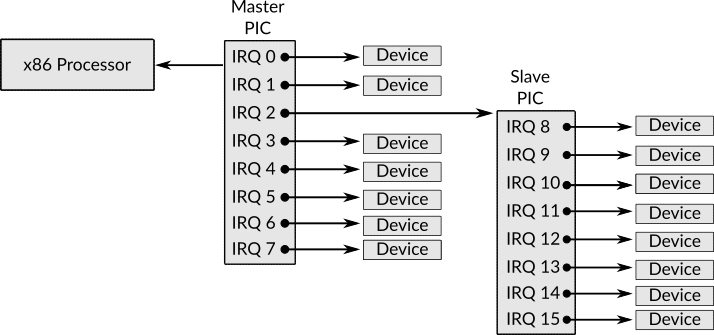
\includegraphics[width=0.50000\textwidth]{Figures/progenitor-ch/Fig21082021_0.png}
\caption{The Arrangement of Master and Slave PICs}\label{fig:21082021_0}
\end{figure}

Figure \ref{fig:21082021_0} shows this arrangement, as you can see, now,
there are \lstinline!15! slots in the whole system instead of only
\lstinline!8! slots. In the master PIC, the third slot
(\lstinline!IRQ2!) is connected to the slave PIC, that is, whatever
interrupt received by slave PIC from the devices that are attached to
it, will be sent to the master PIC through \lstinline!IRQ2!. All other
slots in both master (\lstinline!IRQ0! to \lstinline!IRQ7! but
\lstinline!IRQ2!) and slave PICs (\lstinline!IRQ8! to \lstinline!IRQ15!)
are connected to external devices. There is a standard which tells us
the device type that each \lstinline!IRQ! is dedicated to, for example,
\lstinline!IRQ0! is the interrupt which is received by a device known as
\emph{system timer} which is a device that sends an interrupt in each
unit of time which makes it extremely useful for multitasking
environment as we shall see later when we start discussing process
management, the following table shows the use of each \lstinline!IRQ!
\footnote{Source:
  \url{https://en.wikipedia.org/wiki/Interrupt_request_(PC_architecture)}}.

\begin{longtable}[]{@{}ll@{}}
\toprule
IRQ & Description\tabularnewline
\midrule
\endhead
0 & System Timer\tabularnewline
1 & Keyboard (PS/2 port)\tabularnewline
2 & Slave PIC\tabularnewline
3 & Serial Port 2 (COM)\tabularnewline
4 & Serial Port 1 (COM)\tabularnewline
5 & Parallel Port 3 or Sound Card\tabularnewline
6 & Floppy Disk Controller\tabularnewline
7 & Parallel Port 1\tabularnewline
8 & Real-time Clock\tabularnewline
9 & APCI\tabularnewline
10 & Available\tabularnewline
11 & Available\tabularnewline
12 & Mouse (PS/2 port)\tabularnewline
13 & Coprocessor\tabularnewline
14 & Primary ATA\tabularnewline
15 & Secondary ATA\tabularnewline
\bottomrule
\end{longtable}

After receiving an \lstinline!IRQ! from a device, PIC should send this
request to the processor, in this stage each \lstinline!IRQ! number is
mapped (or translated, if you prefer) to an interrupt number for the
processor, for example, \lstinline!IRQ0! will be sent to the processor
as interrupt number \lstinline!8!, \lstinline!IRQ1! will be mapped to
interrupt number \lstinline!9! and so on until \lstinline!IRQ7! which
will be mapped to interrupt number \lstinline!15d! (\lstinline!0Fh!),
while \lstinline!IRQ8! till \lstinline!IRQ15! will be mapped to
interrupts number from \lstinline!112d! (\lstinline!70h!) to
\lstinline!119d! (\lstinline!77h!).

In the real-mode, this mapping will be fine, but in protected-mode it is
going to cause conflicts between software and hardware interrupts, that
is, one interrupt number will be used by both software and hardware
which may causes some difficulties later in distinguishing the source of
this interrupt, is it from the software or hardware? For example, in
protected mode, interrupt number \lstinline!8! which is used for system
timer interrupt by PIC is also used by the processor when a software
error known as \emph{double fault} occurs. The good thing is that PIC is
\textbf{programmable}, which means that we can send commands to PIC and
tell it to change the default mapping (from \lstinline!IRQs! to
processor's interrupts number) to another mapping of our choice.

There are two well-known types of communicating with external devices by
the processor, we have already encountered one of them when we worked
with video memory which causes the processor to communicate with the
screen to write characters or draw pixels, this type of communication
from the processor to a devices is known as \emph{memory-mapped I/O}
communication, that is, the main memory is used to perform the
communication.

There is another type which is used by PIC and this type is known as
\emph{port-mapped I/O} communication. In this method, each device (that
uses this way) has \emph{ports}, each port has its own unique number and
job, for example, master PIC has two ports, the number of the first port
is \lstinline!20h! while the number of the second port is
\lstinline!21h!, the first port is used to send commands \footnote{Each
  device has its own set of commands.} to master PIC while the second
port is used to write data on it so the master PIC can read it. The same
is applicable to slave PIC with different port numbers, \lstinline!a0h!
and \lstinline!a1h! respectively. PIC has no explicit command to remap
\lstinline!IRQs!, instead, there is a command to initialize PIC, this
initialization consists of multiple steps and one of these steps it is
to set the required mapping. Now, we can present the skeleton of
\lstinline!setup_interrupts! as following.

\begin{lstlisting}
setup_interrupts:
    call remap_pic
    call load_idt
    
    ret
\end{lstlisting}

First, we are going to remap \lstinline!IRQs! to different interrupt
numbers by sending initialization command to both master and slave PICs,
then we are going to initialize and load \lstinline!IDT! and write the
necessary interrupts handlers which are also known as \emph{interrupt
service routines} (ISRs).

\subsection{Remapping PICs}\label{remapping-pics}

As we have said, we need to change the default mapping between
\lstinline!IRQs! and interrupt number of the processor to make sure that
there are no more than one source can emit a signal to one interrupt
number, this process is known as \emph{PIC remapping} which is simple to
perform. As we knew, PIC is a port-mapped I/O, and by using
\lstinline!out! instruction of x86 we can write something on a given
port number.

The \emph{initialization command} of PIC is represented by the number
\lstinline!11h!, which means writing this value on the command port of
PIC by using \lstinline!out! instruction is going to tell the PIC device
that we are going to initialize it. When we send this command to the PIC
through its own command port (\lstinline!20h! for master PIC and
\lstinline!a0h! for slave PIC), it is going to wait for us to write four
parameters on its data port (\lstinline!21h! for master PIC and
\lstinline!a1h! for slave PIC), the values of these parameters are
represented by numbers as we shall see in a moment.

The first parameter that should be provided to initialization command is
the new starting offset of \lstinline!IRQs!, for example, if the value
of this parameter is \lstinline!32d! for master PIC, that means
\lstinline!IRQ0! will be sent to the processor as interrupt number
\lstinline!32d! instead of \lstinline!8d! (as in default mapping),
\lstinline!IRQ1! will be sent to the processor as interrupt number
\lstinline!33d! and so on. The second parameter tells the PIC (that we
are initializing) in which of its slot the other PIC is connected. The
third parameter tells the PIC which mode we would like it to run on,
there are multiple modes for PIC devices, but the mode that we care
about and need to use is x86 mode. The fourth parameter tells the PIC
which \lstinline!IRQs! to enable and which to disable. Now, let's see
the code of \lstinline!remap_pic! routine which implements what we have
just described by setting the correct parameters to the initialization
command of both master and slave PICs.

\begin{lstlisting}
remap_pic:
    mov al, 11h
    
    send_init_cmd_to_pic_master:    
        out 0x20, al
        
    send_init_cmd_to_pic_slave:     
        out 0xa0, al
        
    ; ... ;
    
    make_irq_starts_from_intr_32_in_pic_master:     
        mov al, 32d
        out 0x21, al
    
    make_irq_starts_from_intr_40_in_pic_slave:
        mov al, 40d
        out 0xa1, al 
    
    ; ... ;
    
    tell_pic_master_where_pic_slave_is_connected:
        mov al, 04h
        out 0x21, al
    
    tell_pic_slave_where_pic_master_is_connected:
        mov al, 02h
        out 0xa1, al
    
    ; ... ;
    
    mov al, 01h
    
    tell_pic_master_the_arch_is_x86:
        out 0x21, al
    
    tell_pic_slave_the_arch_is_x86:
        out 0xa1, al
    
    ; ... ;
    
    mov al, 0h
    
    make_pic_master_enables_all_irqs:
        out 0x21, al
    
    make_pic_slave_enables_all_irqs:
        out 0xa1, al
    
    ; ... ;
    
    ret
\end{lstlisting}

Note that the labels here are optional, I've added them for the sake of
readability, you can get rid of them if you want. As you can see, the
command and data port for both master and slave PICs are used to send
initialize command and the parameters. The instruction \lstinline!out!
can only take the register \lstinline!ax! as second operand and due to
that, the number that represent the command or the data that we would
like to send are always set to \lstinline!al! first which is used later
as the second operand of \lstinline!out!. Also, it should be obvious
that the first operand of \lstinline!out! is the port number, while the
second operand is the value that we would like to send.

\begin{figure}
\centering
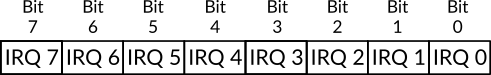
\includegraphics[width=0.50000\textwidth]{Figures/progenitor-ch/Fig27082021_0.png}
\caption{Master PIC's Data Format to Set The Place of Slave
PIC}\label{fig:27082021_0}
\end{figure}

You may ask, why the value is \lstinline!4! is used in the label
\lstinline!tell_pic_master_where_pic_slave_is_connected! \footnote{I
  just realized that this is a really long name! Sorry, sometimes I
  become a readability freak!} instead of \lstinline!2! since we said
earlier that the salve PIC is connected to master PIC through
\lstinline!IRQ2!. The reason of that is the format of the data that
should be sent to master PIC in order to tell it the place where slave
PIC is attached to. This format is shown in figure \ref{fig:27082021_0}
which shows that the size of the data is \lstinline!1! byte and each
\lstinline!IRQ! is represented by one bit, that is, each bit is used as
a flag to indicate which \lstinline!IRQ! we would like to use.

\begin{figure}
\centering
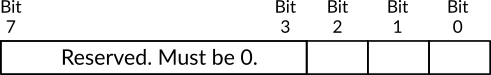
\includegraphics[width=0.50000\textwidth]{Figures/progenitor-ch/Fig27082021_1.png}
\caption{Slave PIC's Data Format to Set The Place of Master
PIC}\label{fig:27082021_1}
\end{figure}

In our case, slave PIC is connected to master PIC through
\lstinline!IRQ2! which is represented by bit \lstinline!2!, which means
the value of this bit should be \lstinline!1! and all other bits should
be \lstinline!0!, this gives us the binary sequence
\lstinline!0000 0100! which is \lstinline!4d!. Assume that the slave PIC
is connect to master PIC through \lstinline!IRQ7!, then the binary
sequence will be \lstinline!1000 0000!, which is \lstinline!128d!. For
the slave PIC, the format is shown in figure \ref{fig:27082021_1} and as
you can see, only bits \lstinline!0! to \lstinline!2! can be used while
the others should be \lstinline!0!. By using these three bits we can
represent the number \lstinline!8! at most, the normal way of
representing the numbers can be used here and for that the value
\lstinline!2! is passed to slave PIC to tell it that it is connected to
master PIC through \lstinline!IRQ2! in the label
\lstinline!tell_pic_slave_where_pic_master_is_connected!.

\subsection{Writing ISRs and Loading
IDT}\label{writing-isrs-and-loading-idt}

Right now, everything is ready to write the code of loading
\lstinline!IDT! and \lstinline!ISR!s. The first one is too simple and
similar to the code of loading the \lstinline!GDT! table, the following
is the code of \lstinline!load_idt! routine.

\begin{lstlisting}
load_idt:
    lidt [idtr - start]
    ret
\end{lstlisting}

As you can see, nothing is new here. The instruction \lstinline!lidt! is
used to load the content of the register \lstinline!idtr! by using the
same way that we have already used in the previous routine
\lstinline!load_gdt!. Now, for the sake of organizing, I'm going to
dedicate a new file for the related stuff of \lstinline!IDT! and
\lstinline!ISR!s and this file will be called \lstinline!idt.asm!. In
the end of \lstinline!starter.asm! the following line should be added
\lstinline!%include "idt.asm"!, exactly as we did with
\lstinline!gdt.asm!.

At least, we need to define \lstinline!49! \lstinline!ISR!s since the
interrupts from \lstinline!0! to \lstinline!31! are used by the
processor to indicate that some error happened in the system. In fact,
interrupts \lstinline!22! to \lstinline!31! are reserved and has no use
for us, but we need to fill their entries in the \lstinline!IDT! table
to be able to use the interrupts starting from \lstinline!32!. While the
interrupts \lstinline!32! to \lstinline!48! are now used by PIC after
the remapping for hardware interrupts (\lstinline!IRQs!). Hence, we need
to fill the entries of all of these interrupts in the \lstinline!IDT! to
make sure that our kernel runs correctly. Right now, we are going to use
the same skeleton for the \lstinline!ISRs! that we are going to define,
let's start with \lstinline!isr_0! which is the name of the routine that
handles interrupt \lstinline!0!. Starting from here, the code that are
presented should be in the file \lstinline!idt.asm! unless otherwise is
mentioned explicitly.

\begin{lstlisting}
isr_0:
    cli
    push 0
    jmp isr_basic
\end{lstlisting}

The code here is too simple, we first make sure that interrupts are
disabled by using the instruction \lstinline!cli!; in the time that we
are handling an interrupt, we don't want another interrupt to occur, it
will be more obvious why this is important when we start to implement
process management in 539kernel.

After disabling the interrupts, we push to the stack the value
\lstinline!0! which is the number of the current interrupt, this pushed
value can be used later by a C function that we are going to call as a
parameter \footnote{That's possible due to the calling convention as we
  have discussed earlier in the previous chapter \ref{ch-x86}.}, in this
way, we can have just one C function that works as an interrupt handler
which receives a parameter that holds the interrupt number which should
be handled. After pushing the interrupt number, the routine is going to
jump to the label \lstinline!isr_basic! which contains the basic code of
all \lstinline!ISRs! that we are going to define.

Now, for all other \lstinline!ISRs! that are related to the processor,
that is, from interrupt \lstinline!1! to \lstinline!31! we are going to
use the exact same code, only two things should be changed, the name of
the routine should indicate the interrupt number, for example
\lstinline!isr_1! for interrupt \lstinline!1!, \lstinline!isr_2! for
\lstinline!2! and so on, the second change is the pushed value. I'm not
going to show you all \lstinline!31! \lstinline!ISR!s in here since they
need a lot of space, but you can always refer to 539kernel source code
if the matter isn't clear for you and the following is an example of
\lstinline!ISRs! \lstinline!1!, \lstinline!2! and \lstinline!3!. The
label \lstinline!isr_basic! will be defined later on.

\begin{lstlisting}
isr_1:
    cli
    push 1
    jmp isr_basic
    
isr_2:
    cli
    push 2
    jmp isr_basic
    
isr_3:
    cli
    push 3
    jmp isr_basic
\end{lstlisting}

The second set of \lstinline!ISR!s is the one that handles the
\lstinline!IRQ!s and the interrupt numbers here, as we mentioned
earlier, starts from \lstinline!32! to \lstinline!48!. The following is
an example of one of them which is \lstinline!isr_32!.

\begin{lstlisting}
isr_32:
    cli
    push 32
    jmp irq_basic
\end{lstlisting}

It's exactly the same code as the \lstinline!ISR!s before
\lstinline!32!, the only difference is the label that will the routine
jumps to. In the current case it is \lstinline!irq_basic!, which is the
basic code for all interrupts that handles the \lstinline!IRQs!, hence,
\lstinline!isr_33! till \lstinline!isr_48! has the same code as
\lstinline!isr_32! but with changing the pushed value. The following is
the code of \lstinline!isr_basic!.

\begin{lstlisting}
isr_basic:
    call interrupt_handler
    
    pop eax
    
    sti
    iret
\end{lstlisting}

Simply, \lstinline!isr_basic! calls a function known as
\lstinline!interrupt_handler! which is a C function that is going to be
in the main kernel code, to make \lstinline!NASM! able to know that this
function is defined elsewhere than the assembly code, the line
\lstinline!extern interrupt_handler! should be added before
\lstinline!start! routine in \lstinline!starter.asm!, exactly as we did
with the function \lstinline!kernel_main!.

After the function \lstinline!interrupt_handler! returns, the stack of
the current \lstinline!ISR! is cleaned by eliminating the value that we
have pushed which represents the number of the current interrupt, this
is performed by using \lstinline!pop! instruction which requires an
operand to store the popped value on it and for no reason I've chosen
\lstinline!eax!. This is a simplest way of cleaning the stack's frame,
another well known way is \lstinline!add esp, 4! where the second
operand is the size of all data that we have pushed on the frame and we
would like to eliminate before return, in our case, the size of the
number that we have pushed is \lstinline!4! bytes. As you can see, the
latter method of cleaning the stack is more preferred since no place to
store the popped value is needed and most probably you are going to
encounter this method in the real codes much more. For the sake of
simplicity, I'm going to keep the earlier method in the current case
unless the other is needed.

Finally, the \lstinline!ISR! re-enables the interrupts with the
instruction \lstinline!sti! and returns by using the instruction
\lstinline!iret! instead of the normal \lstinline!ret! that we have used
before, the former one is the one that should be used by interrupt
handlers to return. The following is the code of \lstinline!irq_basic!.

\begin{lstlisting}
irq_basic:
    call interrupt_handler
    
    mov al, 0x20
    out 0x20, al
    
    cmp byte [esp], 40d
    jnge irq_basic_end
    
    mov al, 0xa0
    out 0x20, al
    
    irq_basic_end:
        pop eax
        
        sti
        iret
\end{lstlisting}

The fundamental functionality of \lstinline!irq_basic! is same as
\lstinline!isr_basic!, it calls the C function
\lstinline!interrupt_handler! and in the end it cleans the stack and
returns (in label \lstinline!irq_basic_end!), the question now, what is
this additional code between calling the C function and returning? As
you know, \lstinline!IRQs! come from one of the PICs of the system, and
this \lstinline!PCI! requires to be told that the \lstinline!IRQ! it
sent has been handled, to do that the PIC command known as \emph{end of
interrupt} (\lstinline!EOI!) should be used and that's what the code
does.

The command \lstinline!EOI! should be sent to the master PIC after
handling all \lstinline!IRQs! (the ones that belong to the master and
also the slave), but for the slave \lstinline!PIC! this command should
be sent only after the \lstinline!IRQs! of slave PIC are handled, that
is, interrupt number \lstinline!40! till \lstinline!48!. So, after
returning from the C function \lstinline!interrupt_handler!, the command
\lstinline!EOI! is sent directly to the mater PIC. As you can see, we
write the value \lstinline!20h! to the port \lstinline!20h!, the first
value represents that \lstinline!EOI! command, while the second value
represents the command port of master PIC as we learned earlier. After
that, the interrupt number, that we have pushed on the stack in the
beginning of the \lstinline!ISR!, is used to check if the interrupt that
we have handled is greater than or equal \lstinline!40d!, if this is not
the case, a jump is performed to \lstinline!irq_basic_end!, otherwise,
\lstinline!EOI! command is sent to the slave PIC through its command
port \lstinline!a0h!.

Now, we are ready to define the \lstinline!IDT! table, to not take too
much space I will show only the first three entries, but the full table
should have \lstinline!49! entries, all of them with the same exact
fields and the only difference is the label name of the \lstinline!ISR!
\footnote{The values of the properties here are used from Basekernel
  project (\url{https://github.com/dthain/basekernel}).}.

\begin{lstlisting}
idt:
    dw isr_0, 8, 0x8e00, 0x0000
    dw isr_1, 8, 0x8e00, 0x0000
    dw isr_2, 8, 0x8e00, 0x0000
\end{lstlisting}

The meaning of the values of the fields are summarized in the following
table.

\begin{longtable}[]{@{}llllll@{}}
\toprule
\begin{minipage}[b]{0.15\columnwidth}\raggedright\strut
Handler's Name\strut
\end{minipage} & \begin{minipage}[b]{0.18\columnwidth}\raggedright\strut
Segment Selector\strut
\end{minipage} & \begin{minipage}[b]{0.09\columnwidth}\raggedright\strut
Present\strut
\end{minipage} & \begin{minipage}[b]{0.16\columnwidth}\raggedright\strut
Privilege Level\strut
\end{minipage} & \begin{minipage}[b]{0.16\columnwidth}\raggedright\strut
Descriptor Size\strut
\end{minipage} & \begin{minipage}[b]{0.11\columnwidth}\raggedright\strut
Gate Type\strut
\end{minipage}\tabularnewline
\midrule
\endhead
\begin{minipage}[t]{0.15\columnwidth}\raggedright\strut
isr\_0\strut
\end{minipage} & \begin{minipage}[t]{0.18\columnwidth}\raggedright\strut
8 (Kernel's Code)\strut
\end{minipage} & \begin{minipage}[t]{0.09\columnwidth}\raggedright\strut
Yes\strut
\end{minipage} & \begin{minipage}[t]{0.16\columnwidth}\raggedright\strut
0\strut
\end{minipage} & \begin{minipage}[t]{0.16\columnwidth}\raggedright\strut
32-bit\strut
\end{minipage} & \begin{minipage}[t]{0.11\columnwidth}\raggedright\strut
Interrupt\strut
\end{minipage}\tabularnewline
\begin{minipage}[t]{0.15\columnwidth}\raggedright\strut
isr\_1\strut
\end{minipage} & \begin{minipage}[t]{0.18\columnwidth}\raggedright\strut
8 (Kernel's Code)\strut
\end{minipage} & \begin{minipage}[t]{0.09\columnwidth}\raggedright\strut
Yes\strut
\end{minipage} & \begin{minipage}[t]{0.16\columnwidth}\raggedright\strut
0\strut
\end{minipage} & \begin{minipage}[t]{0.16\columnwidth}\raggedright\strut
32-bit\strut
\end{minipage} & \begin{minipage}[t]{0.11\columnwidth}\raggedright\strut
Interrupt\strut
\end{minipage}\tabularnewline
\begin{minipage}[t]{0.15\columnwidth}\raggedright\strut
isr\_2\strut
\end{minipage} & \begin{minipage}[t]{0.18\columnwidth}\raggedright\strut
8 (Kernel's Code)\strut
\end{minipage} & \begin{minipage}[t]{0.09\columnwidth}\raggedright\strut
Yes\strut
\end{minipage} & \begin{minipage}[t]{0.16\columnwidth}\raggedright\strut
0\strut
\end{minipage} & \begin{minipage}[t]{0.16\columnwidth}\raggedright\strut
32-bit\strut
\end{minipage} & \begin{minipage}[t]{0.11\columnwidth}\raggedright\strut
Interrupt\strut
\end{minipage}\tabularnewline
\bottomrule
\end{longtable}

As in \lstinline!GDT! table, I've written a Python script that let you
manipulate the properties of descriptors by getting a human readable
input, the code of the script is the following.

\begin{lstlisting}[language=Python]
import json;

def generateIDTAsWords( idtAsJSON, nasmFormat = False ):
    idt = json.loads( idtAsJSON );
    idtAsWords = '';
    
    for entry in idt:
        if nasmFormat:
            idtAsWords += 'dw ';
        
        # ... #
        
        present = ( 1 if entry[ 'present' ] else 0 ) << 7;
        dpl = entry[ 'dpl' ] << 6;
        size = ( 1 if entry[ 'gate_descriptor_size' ] == '32-bit' else 0 ) << 3;
        gateType = ( 0 if entry[ 'interrupt_gate' ] else 1 );
        
        byteFive = present | dpl | ( 0 << 11 ) | size | ( 1 << 2 ) | ( 1 << 1 ) | gateType;
        
        wordThree = '0x' + format( byteFive, 'x' ).zfill( 2 ) + '00';
        
        # ... #
        
        idtAsWords += entry[ 'isr_routine_name' ] + ', ' + str( entry[ 'isr_segment_selector' ] ) + ', ' + wordThree + ', 0x0000'  + '\n';
        
    return idtAsWords;
\end{lstlisting}

The following is an example of using \lstinline!generateIDTAsWords!.

\begin{lstlisting}[language=Python]
idt = '''
[
    {   "isr_routine_name": "isr_0", "isr_segment_selector": 8, "present": true, "dpl": 0, "gate_descriptor_size": "32-bit", "interrupt_gate": true },
    {   "isr_routine_name": "isr_1", "isr_segment_selector": 8, "present": true, "dpl": 0, "gate_descriptor_size": "32-bit", "interrupt_gate": true }
]
''';

print( generateIDTAsWords( idt, True ) );
\end{lstlisting}

After defining the entries of \lstinline!IDT!, we can define the label
\lstinline!idtr! which will be the value that we will load in the
special register \lstinline!idtr!.

\begin{lstlisting}
idtr:
    idt_size_in_bytes   :   dw idtr - idt
    idt_base_address    :   dd idt
\end{lstlisting}

It should be easy to you now to know why \lstinline!idtr - idt! gives us
the size of \lstinline!IDT! in bytes. Also, you should know that if the
label \lstinline!idtr! is not right below the label \lstinline!idt! this
will not work. I've used this method instead of hardcoding the size of
the table \lstinline!8 * 49 = 392! in the code to make sure that I don't
forget to change the size field when I add a new entry in
\lstinline!IDT!, you are free to hardcode the size as we did in
\lstinline!gdtr! if you like to. Finally, the C function
\lstinline!interrupt_handler! can be defined in the end of
\lstinline!main.c! as following.

\begin{lstlisting}[language=C]
void interrupt_handler( int interrupt_number )
{
    println();
    print( "Interrupt Received " );
    printi( interrupt_number );
}
\end{lstlisting}

It simply receives the interrupt number as a parameter, as you have
expected, and prints this number in an appealing way.

And now we have got the progenitor of 539kernel! Compiling and running
this code is going to print the messages
\lstinline"Welcome to 539kernel!" then
\lstinline!We are now in Protected-mode! then \lstinline!539! and
finally, our first interrupt will be received and the message
\lstinline!Interrupt Received 32! will be printed on the screen, this
interrupt will not be received just once since it is the interrupt of
the system timer the kernel will keep receiving it and prints the same
message every given unit of time. We will use the system timer later
when we start discussing the scheduling of processes in chapter
\ref{ch-progenitor}.

\section{Quick View of the Changes of
Makefile}\label{quick-view-of-the-changes-of-makefile}

As you may have noticed, the \lstinline!Makefile! of the progenitor
version of 539kernel has some different aspects than the one that we
have used in the bootloader version of 539kernel. The first difference
is the way that we assemble \lstinline!starter.asm!, as you can see,
unlike \lstinline!bootstrap.asm!, the output of the process of
assembling the starter is an \lstinline!ELF32! binary file instead of
flat binary file. As you know, the code of the starter is related to the
C code of 539kernel, that is, there are C functions that are called in
the starter code. To make the starter able to reach this C code
correctly, the binary output of both \lstinline!starter.asm! and
\lstinline!main.c! should be linked. It is the responsibility of the
linker to generate a final binary file that understands what the starter
mean when it calls the C function \lstinline!interrupt_handler! for
example. If the linking process between the two files is not performed,
the starter will never know where is the code of
\lstinline!interrupt_handler! or \lstinline!kernel_main!.

To link two binary files, they should have the same format and this
format makes it possible to link the files that generated by using it.
GCC generates \lstinline!ELF! binary files by default, so, when we
assemble \lstinline!starter.asm! we tell \lstinline!NASM! to generate
and \lstinline!ELF! file. After that the output binary files (AKA:
object files) of both \lstinline!starter.asm! and \lstinline!main.c! are
linked by using the command \lstinline!ld!, we tell the linker that we
are linking \lstinline!ELF! object files, the order of the files that we
pass to the linker to link is important, as you can see
\lstinline!starter.o! is passed before \lstinline!kernel.elf!, which
makes the linker puts the code of the starter before the code of the
main kernel in the final output \lstinline!ELF! binary file
\lstinline!539kernel.elf!. Because \lstinline!ELF! is not understandable
by the machine unless some code interprets it, we convert it to a flat
binary file by using the command \lstinline!objcopy!, in this way, the
bootloader can load the kernel without the need of dealing with the
details of \lstinline!ELF! format.

Also, you can see that the final image of the kernel
\lstinline!kernel.img! is generated by writing the content of bootloader
first, then the kernel and then the image is fill with around
\lstinline!1MB! of zeros, while this step isn't necessary for QEMU, but
if you decide to use Bochs instead, such a step is required. While we
are going to stick with the former one right now, the latter one, in my
humble opinion, has better debugging tools.

Another important aspect of the new \lstinline!Makefile! is the flags
that are passed to GCC, we need to be careful with these flags and pass
the correct ones to make sure that GCC compiles our kernel correctly
since GCC compiles user-space applications by default. The flag
\lstinline!-Wall! tells GCC to show us the warnings on our code. The
flag \lstinline!-m32! makes GCC generate \lstinline!32-bit! code. The
flag \lstinline!-c! stops the linker from running by default since we
are going to run it later manually with specific options as you have
seen. The flag \lstinline!-ffreestanding! indicates that we are
compiling a code that the standard library of C is not available for it
and the \lstinline!main! function is not necessary for it. Both flags
\lstinline!-fno-asynchronous-unwind-tables! and \lstinline!-fno-pie! are
used to eliminate some extra code that is generated by the GCC to handle
some situations that are related to user-space code. This is a quick
review of the functionality of the flags and you can always refer to the
official documentation of GCC for more details.

\section{A Traditionalist Implementer or a
Kernelist?}\label{a-traditionalist-implementer-or-a-kernelist}

Most probably you are objecting, ``\textbf{kernelist} is not even a
word!'' I know, even my poor spell checker is shocked! Just bear with me
a little bit and let me show you what I mean by the term
\emph{kernelist}.

In our journey of creating an operating system kernel we may ask
ourselves, what is our role exactly? There are two possible roles that I
would like to focus on, the first one is being a traditionalist
implementer (for short: traditionalist). What I mean by the
traditionalist is the one who writes the code of the kernel without
focusing too much on the design of the kernel and the philosophical
questions about that kernel, examples of these questions are ``What is
the problem that the kernel will solve?'', ``How to design its
architecture to accomplish its goal'' and so on, also the traditionalist
tends to implement already well-known solutions that have been used many
years with no or little changes. The kernelist, on the other hand, is
the person who takes care of the questions about kernel's design and the
new solutions for the problems and tries to answer these questions and
presents a suitable kernel's design and solutions for specific problems.
For example, writing a Unix-like kernel is the job of traditionalist,
since the architecture of Unix is already designed by kernelists to
solve specific problems.

Our goal from this book is to \textbf{learn} how to write an operating
system kernel with a traditional design and no new ideas, so, we are
taking the role of a traditionalist, the design of 539kernel is too
simple and it solves no specific problem in a novel way, instead it uses
the concepts that are already there and used by many operating systems
as you will see in the next chapters, also it doesn't focus on some new
problem to solve nor a new solution for an old problem, this makes
539kernel a working kernel that solves the same problems that other
kernels solve by using the same methods that other kernels use, the
advantage of this design is making 539kernel easy to implement which
means it is a good starting point to learn about operating system
kernels and that's the goal of this book.

The natural question for someone, who would like to continue in the
journey of operating system kernels, to ask herself after implementing a
basic kernel, ``What's next?'' and here where a kernelist is born! In
fact, there are many real world problems in computing that need to be
solved, also, there are many innovative ideas that need to be created,
furthermore, there are many good ideas that have been presented by
someone else but need to be realized in the real world systems, a lot of
aforementioned can be found in the scientific papers \footnote{In fact,
  I've started a project that generalize this thought and I called it
  \lstinline!ResearchCoders!. If you are interested in finding and
  implementing new ideas that solve real-world problems you may would
  like to check the website of the project
  (\url{https://researchcoders.dev})}.

The kernelist doesn't necessarily innovate new solutions by himself, but
he can use modern solutions that have been proposed by other kernelist
to implement and design a kernel with modern innovative and useful ideas
instead of reimplementing the traditional solutions that have been with
us for \lstinline!60! years over and over again.

After reading this book to learn about creating a kernel and you would
like to continue the journey, I encourage you to consider the role of
kernelist. Using what you have learned to solve real-world problem is a
good idea, and the world needs this kind of orientation. Although this
is a book of traditionalist more that a kernelist, I've dedicated
chapter \ref{ch-wthat-is-next} for those who would like to, at least,
take a look on being kernelist.

    \chapter{Chapter 4: Process Management}\label{ch-process-management}

\section{Introduction}\label{introduction}

In the previous chapters, we have discussed the topics that helped us to
understand the basics that are needed to initialize the environment for
a \lstinline!32-bit! protected mode kernel running on x86. Starting from
this chapter we are going to discuss the topics that belong to the
kernel itself, that is, the responsibilities of the kernel. We will
start with a quick look on the theories that are traditionally presented
on academic textbooks, then we move to the practical part in order to
implement these theories (or part of them) in 539kernel. A good place to
start from is \emph{process management}.

A kernel has multiple responsibilities, one of these responsibilities is
to manage the resources and make sure they are managed well. One
important resource of the computers is the time of the processor (AKA:
CPU time) which is the component that executes the code of software that
we would like to run on our machines. Process management is the the part
that studies how a kernel should manage and distribute CPU time among a
bunch of \emph{processes}.

\section{The Most Basic Work Unit: A
Process}\label{the-most-basic-work-unit-a-process}

\emph{Process} is the term which is used in operating systems literature
to describe a running program. In the previous chapters of this book we
have encountered the concept of the process multiple times and you may
recall from these encounters that every user-space software that we use
in our computers is a soulless sequence of bytes that are stored
somewhere in the hard disk. When we decide to use a specific software,
for example, the web browser, the first thing we do is to open it either
through double clicking on its icon in graphical user interfaces or
through writing its command in the shell. When we do that, the kernel is
needed to be called through a \emph{system call} and takes the
responsibility of ``opening'' this software, we can consider system
calls as functions which are provided by the kernel to expose its
services for the user-space software, one way of implementing system
calls is to use interrupts, exactly the same way that we have used with
BIOS.

However, there are multiple steps that are needed to be performed to
open the software, for example, reading its data from disk, but our
current focus is on process-related parts, eventually, the kernel
creates a new process for the software that we requested to open. The
kernel maintains a table of all system processes, each entry represents
a process and contains the information which is needed by the kernel to
manage the process, this data structure which stores a process
information is known as \emph{process control block} (PCB), so, the
processes table will have a process control block as an entry for each
process in the system.

Of course, the most important part of the process is the code of the
software that this process represents and its data, both data \footnote{We
  mean static data here, which are contained in the binary file of the
  software. While the data that are generated by the running process are
  not loaded from the binary file, instead they are created while the
  code is running (e.g.~local variables in the stack).} and code should
be loaded into memory, after that, its code can be executed by the
processor. We need to note that a process is an instance of a software,
in other words, one software can be opened more than one time with a
separated process for each one, for example, opening multiple windows of
the web browser on the same time, the software is one which is the web
browser and it is represented by the binary file which is stored in the
hard disk, but each opened window is a separated process and each
process' content is stored in the main memory. While the described
concept is well-known by the term ``process'', specially in the
literature, other terms can be used for the same concept, for example
\emph{task} and \emph{job} are other words which are used to point to
the same concept.

Each process is known to have a \emph{state}, when it is loaded to the
memory its state will be indicated by the kernel as \emph{ready} and can
be run anytime, when the CPU time is given to a process its state will
be \emph{running}. Also, the state of the process can be \emph{waiting},
an example of a situation where a process state is changed to waiting
state is when it performs I/O request (e.g.~read from the hard disk),
its state will be \emph{waiting} since it's waiting for the I/O device
to fulfill the request. The state information about a process is stored
in the process control block which is, as mentioned earlier, an entry in
the processes table.

Sometimes, a bunch of processes in a system need to communicate with
each other to share some data or tell each other to perform a specific
operation, this led to a broad topic known as \emph{inter-process
communication} (IPC) which provides mechanisms to make this type of
communication possible. The applications of \lstinline!IPC! is not
restricted to operating system kernels, they are used in distributed
computing for instance. One well known mechanism of \lstinline!IPC! is
\emph{shared memory}, that is, a region of the memory is made accessible
by more than one process, they can read and write to this region in
order to share data. The ability to write to same place by more than one
process can cause a problem known as \emph{race condition}, given a
shared variable, the situation which two or more processes try to change
the value of this variable at the same moment is known as race
condition. There are multiple solutions for this problem and this topic
is studied in a branch known \emph{concurrency control} which is a
shared topic by many applications, one of them is database management
systems (DBMS) which needs these mechanisms when two users try to update
the same row at the same time.

Processes are not the only entities that need to communicate, there is
another unit of work which is known as \emph{thread} and it can be
described as lightweight process. A process can have more than one
thread and when a software uses more than one thread to do its job, it
is described as \emph{multithreaded}. Threads are everywhere in our
usage of computers, and a world without them is unimaginable. For
example, when you use a text editor, the main thread of the software
lets you write your text, but when you click on save icon a separated
thread within the text editor's process is used to perform this
operation. Furthermore, another thread can be used for the spell checker
while you are typing. If all there functionalities were on one thread,
you will need to wait each one of them to finish in order to let you to
perform the other functionality, that is, the software without threads
is going to run sequentially while threads provide us concurrency within
one process. Threads and processes have many similarities, for example,
both of them are there to be executed, hence, they need to use the
processor and both of them need to be scheduled to give every one of
them time from the processor. In contrast to processes, threads run as a
part of same process and they share the same address space which makes
the communication between them much easier since they can reach the same
memory by default.

\section{The Basics of Multitasking}\label{the-basics-of-multitasking}

When we write a kernel, multiple design questions should be answered
\footnote{Remember the job of a kernelist!} and the part of process
management is not an exception of that. There are multiple well-known
answers for some basic design questions, each one of those answers tries
to solve a problem that faced the person who gave us this answer, for
example, one of well-known features of the modern operating systems is
\emph{multitasking} which is the successor of \emph{monotasking} and
both of them can be considered as answers for a design question in
operating systems. In multitasking environment, the system can run
multiple processes at the same time even if there is only one processor
available, while in monotasking environment, the system can run only one
process at a time until this process finishes its work or the user
closes it, only after that, another process can be run.

\subsection{Mutliprogramming \&
Time-Sharing}\label{mutliprogramming-time-sharing}

In the days of monotasking, we were facing a serious problem that led to
the birth of multitasking. It has been noticed that the processes tend
to have idle time, for example, when the process is waiting for the hard
disk to fetch some stored data, the process will be idle while it is
taking over the processor, that is, the processor is under the process'
control which is currently doesn't use the CPU time for something
useful, that means, in this case, we are wasting the valuable resource
of CPU time in waiting for some action to finish, we need to utilize the
processor as much as possible, and here came the solution of this
problem by letting the kernel to have a list of processes that are
\emph{ready} to run.

Assuming the machine has just one processor with one core, the CPU time
will be given to, say process \lstinline!A!, for some time and at some
point of running time the process \lstinline!A! requests from the disk
some data and due to that it becomes idle waiting for disk to respond.
Instead of keep the control of the processor under the process
\lstinline!A!, which is doing nothing but waiting right now, the kernel
suspends process \lstinline!A! and gives the CPU time to another ready
process, say process \lstinline!B!, this switching between two processes
is known as \emph{context switch}. The process \lstinline!B! is going to
use the processor while process \lstinline!A! is waiting for the disk to
respond. At some point, process \lstinline!B! will perform some action
that makes it idle which means that the kernel can switch to another
ready process and so on. This solution is known as
\emph{multiprogramming}. To sum it up, we have a list of ready
processes, choose one, give it the CPU time and wait for it until it
becomes idle, since it's waiting for something switch to another process
which is not idle an so on.

Better yet, multiprogramming has been extended to utilize the processor
more efficiently. Instead of waiting for the currently running process
to perform something which makes it idle, why don't we suspend it after
some period of running time whether it is idle or not and switch to
another process? This solution is known as \emph{time sharing} which is
with multiprogramming represent the scheme that modern operating systems
use for multitasking. In time sharing, a list of ready processes is
available for the kernel, in each unit of time, say for example, every
\lstinline!1! second (in practice, it is shorter) the currently running
process is suspended by the kernel and another process is given the CPU
time and so on.

\subsection{Process Scheduling}\label{process-scheduling}

You may recall from the previous chapter \ref{ch-progenitor} the system
timer which emits an interrupt every unit of time, this interrupt can be
used to implement time sharing in order to switch between the processes
of the system, of course the kernel needs an algorithm to choose which
process to run next, this kind of algorithms are known as
\emph{scheduling algorithms} and in general this part of the topic is
known as \emph{scheduling} in which we try to find the best way of
choosing the next process to run in order to satisfy our requirements.

The \emph{scheduler} is the part of the kernel that schedules the next
process by using some specific scheduling algorithm, that is, it decides
the next process to run based and performs the context switching. There
are many scheduling algorithms to deal with different requirements and
one of them is known as \emph{round-robin}. In this algorithm, each
process is given a fixed amount of CPU time known as \emph{quantum},
when the running process finishes its quantum the scheduler will be
called and the CPU time will be given to the next process in the list
until its quantum finishes and so on until the schedule reaches to the
end of the process list where it starts with the first process again.
The value of the quantum is decided by the kernelist, for example
\lstinline!50! milliseconds, which means each process will run
\lstinline!50! milliseconds then suspended to run the next one on the
list and so on.

\subsection{Process Context}\label{process-context}

As you know, when a process is executing, it can use the registers of
the processor (e.g. \lstinline!EAX!) to store its own data. Also, it may
change the values of segment registers in case it is running under a
system that employs segmented-memory instead of flat memory model.
Furthermore, the value of the instruction pointer \lstinline!EIP! will
contain an address which belong to the process' address space. All these
values that are related to a process and stored inside the registers of
the processor are known as \emph{process context}, another term which is
\emph{process state} may also be used in some places to mean the same
thing, but to not confuse this concept with the one that we have defined
the term ``state'' with previously, it is better to use the term process
context.

When a scheduler decides to change the currently running process, let's
call it \lstinline!A!, through a context switch, a copy of the context
of the process \lstinline!A! should be taken and stored somewhere, that
is, a snapshot of the last context of \lstinline!A! is taken before
switching to another process. By taking this snapshot, it will be easy
later to resume process \lstinline!A! by just loading its context to the
processor's register and jump to the the value of \lstinline!EIP! which
has been just loaded.

\subsection{Preemptive \& Cooperative
Multitasking}\label{preemptive-cooperative-multitasking}

Both multiprogramming and time-sharing solutions give us a type of
multitasking known as \emph{preemptive multitasking}, the processes are
forced by the kernel to give the CPU time to another process and no
process can take over the processor for the whole time. Another type of
multitasking is known as \emph{cooperative multitasking} (or
\emph{non-preemptive multitasking}), in this type the context switching
is not perform forcibly, instead, the currently running process should
cooperate and voluntarily tells the kernel when it should be suspended
and a context switch should be performed. One of the obvious problems of
this way, at least for the well-known workloads (e.g.~servers or
desktops), that a process, which runs a code that has been written by
someone we don't know, cannot be trusted. It simply may take over the
CPU time and never cooperate and give it up due to an error in the code
or even in purpose \footnote{You may ask who would use cooperative
  multitasking and give this big trust to the code of the software! In
  fact, the versions of Windows before 95 used this style of
  multitasking, also, Classic Mac OS used it. Why? You may ask, I don't
  know exactly, but what I know for sure is that humanity is in a
  learning process!}.

\section{Multitasking in x86}\label{multitasking-in-x86}

With the assistance of system timer, multitasking can be realized fully
by the kernel, that is, by the code. This type is known as
\emph{software multitasking}, the kernel itself is responsible for
storing the list of processes and their related information, also, it's
responsible for storing a snapshot of process context before performing
context switching and resuming this snapshot when the process is
resumed. On the other hand, In x86 some features are provided to handle
these things with the assistance of the processor itself, this type is
known as \emph{hardware multitasking}.

While hardware multitasking is available in x86, the modern operating
system kernels don't use it, instead, multitasking is implemented by the
kernel itself. One reason to take this decision is portability. Modern
kernels tend to run on more than one architecture and not only x86, by
using as little as possible of architecture's features it will be easier
to port a kernel to other architectures.

In this section, we are going to cover the basics of hardware
multitasking in x86 which are needed to initialize the environment to
make it work correctly, in the same way as \lstinline!GDT! with flat
memory model. Furthermore, I think knowing the other available options
is important, especially for kernelists. In 539kernel we are going to to
implement software multitasking as in modern kernels.

\subsection{Task-State Segments}\label{task-state-segments}

The most basic component of hardware multitasking in x86 is known as
\emph{task-state segment} (TSS) \footnote{In x86, the term task is used
  instead of process.} which is a segment in the memory as any other
code or data segment, it has what other segments have, a base address, a
limit and properties. The difference from code and data segments is that
\lstinline!TSS! is a system segment \footnote{In chapter \ref{ch-x86} we
  have seen that there are two types of segments in x86, application
  segments such as code, data and stack segment. And system segments and
  they are \lstinline!LDT! and \lstinline!TSS!.}, this segment stores
the context of a specific process.

In hardware multitasking, each process should has its own
\lstinline!TSS!, and each \lstinline!TSS! should has an entry in the
\lstinline!GDT! table, that is, \emph{TSS descriptor}. A special
register known as \emph{task register} should contain the segment
selector of the currently running process's \lstinline!TSS! descriptor,
the instruction \lstinline!ltr! is used to store a value in this
register.

\hypertarget{fig:tss}{
\begin{figure}
\centering
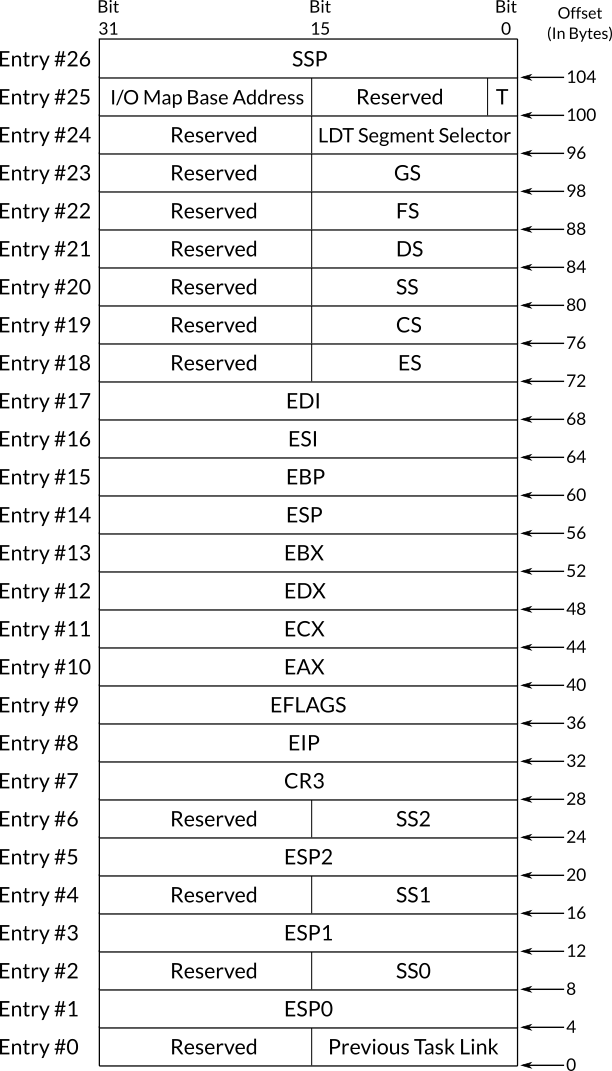
\includegraphics[width=0.45000\textwidth]{Figures/process-ch/tss.png}
\caption{Figure 1: The Structure of Task-State Segment}\label{fig:tss}
\end{figure}
}

Figure \protect\hyperlink{fig:tss}{1} shows the structure of a
task-state segment, as you can see, most of the fields are values of
registers while the others are out of our topic's range except for
previous task link which will be covered in a moment. You can see that
stack segment register and stack pointer register have four entries
instead of one, \lstinline!SS!, \lstinline!SS0!, \lstinline!SS1! and
\lstinline!SS2! for stack segment register. \lstinline!ESP!,
\lstinline!ESP0!, \lstinline!ESP1! and \lstinline!ESP2! for stack
pointer register. These fields point to the stack that should be used
when the process is in a specific privilege level, for example,
\lstinline!SS0:ESP0! will be used as the stack of the process when it
switches to privilege level \lstinline!0!, when it switches back to
privilege level \lstinline!3! the stack \lstinline!SS:ESP! will be used
instead, and the same is applicable to the other similar fields. If we
intend to implement software multitasking, the sole reason of defining
at least one \lstinline!TSS! is due to these fields, when a switch
between privilege levels occurs, the processor needs a \lstinline!TSS!
to use these fields from it in order to switch between stacks. This is
needed only when the system runs user-space code, that is, privilege
level \lstinline!3! code.

The structure of \lstinline!TSS! descriptor in \lstinline!GDT! table is
same as the segment descriptor that we have already explained in chapter
\ref{ch-x86}. The only difference is in the \emph{type field} which has
the static binary value \lstinline!010B1! in \lstinline!TSS! descriptor
where \lstinline!B! in this value is known as \lstinline!B! flag, or
\emph{busy flag} which should be \lstinline!1! when the process that
this TSS descriptor represents is active and \lstinline!0! when it is
inactive.

\subsection{Context Switching in x86}\label{context-switching-in-x86}

One way of switching from a process to another \footnote{In x86, context
  switch is known as task switch.} in x86 hardware multitasking is to
call or jump to TSS descriptor in \lstinline!GDT!, assume that the
system timer caused the call of the scheduler which selects process
\lstinline!A! as the next process to run, the scheduler can cause
context switch by using the instructions \lstinline!call! or
\lstinline!jmp! and the operand should be the segment selector of
\lstinline!A!'s TSS descriptor. In this way, the processor is going to
take a copy of currently running process (call it \lstinline!B!) and
store it in \lstinline!B!'s own \lstinline!TSS!, then the values in
\lstinline!A!'s TSS will be loaded into the processor registers and then
execution of \lstinline!A! begins.

Another way of context switching in x86 hardware multitasking is to call
or jump to a task gate. In chapter \ref{ch-x86}, when we discussed the
descriptors of \lstinline!IDT!, we have said that one type of descriptor
that can be defined is a task gate descriptor. This kind of descriptors
is considered as a separated process by the processor, when we jump or
call a task gate, the previously explained mechanism of task switching
will be performed. Task gates can also be defined in \lstinline!GDT! and
\lstinline!LDT!. In the \lstinline!IDT! table of 539kernel we have
chosen to not define the interrupts as task gates, we don't want to
perform a context switch with each interrupt.

When a process is called instead of jumped to, eventually, it should
return to the caller process by using the instruction \lstinline!iret!,
for the processor, to be able to decide which task is the caller, the
previous task link field of the callee's \lstinline!TSS! will be updated
to contain the segment selector of the caller process. In this way, when
\lstinline!iret! instruction is executed, it will be easy to know to
which process the processor should switch back to.

\section{Process Management in
539kernel}\label{process-management-in-539kernel}

The final result of this section is what I call version \lstinline!T! of
539kernel which has a basic multitasking capability. The multitasking
style that we are going to implement is time-sharing multitasking. Also,
instead of depending on x86 features to implement multitasking in
539kernel, a software multitasking will be implemented. The final
\lstinline!Makefile! of version \lstinline!T! is provided in the last
subsection, however, if you wish to build and run the kernel
incrementally after each change on the progenitor you can refer to that
\lstinline!Makefile! and add only the needed instructions to build the
not ready yet version \lstinline!T! that you are building. For example,
as you will see in a moment new files \lstinline!screen.c! and
\lstinline!screen.h! will be added in version \lstinline!T! as a first
increment, to run the kernel after adding them you need to add the
command to compile this new file and link it with the previous files,
you can find these commands in the last version of \lstinline!Makefile!
as we have said before.

Our first step of this implementation is to setup a valid task-state
segment, while 539kernel implements a software multitasking, a valid TSS
is needed. As we have said earlier, it will not be needed in our current
stage but we will set it up anyway. Its need will show up when the
kernel lets user-space software to run. After that, basic data
structures for process table and process control block are implemented.
These data structures and their usage will be as simple as possible
since we don't have any mean for dynamic memory allocation, yet! After
that, the scheduler can be implemented and system timer's interrupt can
be used to enforce preemptive multitasking by calling the scheduler
every period of time. The scheduler uses round-robin algorithm to choose
the next process that will use the CPU time, and the context switching
is performed after that. Finally, we are going to create a number of
processes to make sure that everything works fine.

Before getting started in the plan that has been just described, we need
to organize our code a little bit since it's going to be larger starting
from this point. New two files should be created, \lstinline!screen.c!
and its header file \lstinline!screen.h!. We move the printing functions
that we have defined in the progenitor and their related global
variables to \lstinline!screen.c! and their prototypes should be in
\lstinline!screen.h!, so, we can \lstinline!include! the latter in other
C files when we need to use the printing functions. The following is the
content of \lstinline!screen.h!.

\begin{lstlisting}[language=C]
volatile unsigned char *video;

int nextTextPos;
int currLine;

void screen_init();
void print( char * );
void println();
void printi( int );
\end{lstlisting}

As you can see, a new function \lstinline!screen_init! has been
introduced while the others are same as the ones that we already wrote.
The function \lstinline!screen_init! will be called by the kernel once
it starts running, the function initializes the values of the global
variables \lstinline!video!, \lstinline!nextTextPos! and
\lstinline!currLine!. Its code is the following and it should be in
\lstinline!screen.c!, of course in the beginning of this file,
\lstinline!screen.h! should be included by using the line
\lstinline!#include "screen.h"!.

\begin{lstlisting}[language=C]
void screen_init()
{
    video = 0xB8000;
    nextTextPos = 0;
    currLine = 0;
}
\end{lstlisting}

Nothing new in here, just some organizing. Now, the prototypes and
implementations of the functions \lstinline!print!, \lstinline!println!
and \lstinline!printi! should be removed from \lstinline!main.c!.
Furthermore, the global variables \lstinline!video!,
\lstinline!nextTextPos! and \lstinline!currLine! should also be removed
from \lstinline!main.c!. Now, the file \lstinline!screen.h! should be
included in \lstinline!main.c! and in the beginning of the function
\lstinline!kernel_main! the function \lstinline!screen_init! should be
called.

\subsection{Initializing the Task-State
Segment}\label{initializing-the-task-state-segment}

Setting TSS up is too simple. First we know that the TSS itself is a
region in the memory (since it is a segment), so, let's allocate this
region of memory. The following should be added at end of
\lstinline!starter.asm!, even after including the files
\lstinline!gdt.asm! and \lstinline!idt.asm!. In the following a label
named \lstinline!tss! is defined, and inside this region of memory,
which its address is represented by the label \lstinline!tss!, we put a
doubleword of \lstinline!0!, recall that a word is \lstinline!2! bytes
while a double-word is \lstinline!4! bytes. So, our \lstinline!TSS!
contains nothing but a bunch of zeros.

\begin{lstlisting}
tss:
    dd 0
\end{lstlisting}

As you may recall, each \lstinline!TSS! needs an entry in the
\lstinline!GDT! table, after defining this entry, the TSS's segment
selector can be loaded into the task register. Then the processor is
going to think that there is one process (one \lstinline!TSS! entry in
\lstinline!GDT!) in the environment and it is the current process (The
segment selector of this \lstinline!TSS! is loaded into task register).
Now, let's define the TSS entry in our \lstinline!GDT! table. In the
file \lstinline!gdt.asm! we add the following entry at the end of the
label \lstinline!gdt!. You should not forget to modify the size of
\lstinline!GDT! under the label \lstinline!gdt_size_in_bytes! under
\lstinline!gdtr! since the sixth entry has been added to the table.

\begin{lstlisting}
tss_descriptor: dw tss + 3, tss, 0x8900, 0x0000
\end{lstlisting}

Now, let's get back to \lstinline!starter.asm! in order to load TSS'
segment selector into the task register. In \lstinline!start! routine
and below the line \lstinline!call setup_interrupts! we add the line
\lstinline!call load_task_register! which calls a new routine named
\lstinline!load_task_register! that loads the task register with the
proper value. The following is the code of this routine that can be
defined before the line \lstinline!bits 32! in \lstinline!starter.asm!.

\begin{lstlisting}
load_task_register:
    mov ax, 40d
    ltr ax
    
    ret
\end{lstlisting}

As you can see, it's too simple. The index of TSS descriptor in
\lstinline!GDT! is
\lstinline!40 = (entry 6 * 8 bytes) - 8 (since indexing starts from 0)!.
So, the value \lstinline!40! is moved to the register \lstinline!AX!
which will be used by the instruction \lstinline!ltr! to load the value
\lstinline!40! into the task register.

\subsection{The Data Structures of
Processes}\label{the-data-structures-of-processes}

When we develop a user-space software and we don't know the size of the
data that this software is going to store while it's running, we usually
use dynamic memory allocation, that is, regions of memory are allocated
at run-time in case we need to store more data that we didn't know that
it will be needed to be stored. We have encountered the run-time stack
previously, and you may recall that this region of memory is dedicated
for local variables, parameters and some information that make function
invocation possible.

The other region of a process is known as run-time heap, which is
dedicated for the data that we decided to store in memory while the
software is running. In C, for instance, the function \lstinline!malloc!
is used to allocate bytes from the run-time heap and maintains
information about free and used space of the heap so in the next use of
this function the allocation algorithm can decide which region should be
allocated based on the required bytes to allocate.

This part that allocates memory dynamically (inside run-time heap) and
manages the related stuff is known as \emph{memory allocator} and one of
well-known allocators is Doug Lea's memory allocator. For programming
languages that run the program by using a virtual machine, like Java and
C\#, or by using interpreters like PHP and Python, they usually provide
their users an automatic dynamic memory allocation instead of the manual
memory allocation which is used by languages such as C, that is, the
programmer of these languages don't need to explicitly call a function
(such as \lstinline!malloc!) to allocate memory in the heap at run-time,
instead, the virtual machine or the interpreter allocates dynamic memory
by itself and frees the region of the heap that are not used anymore
through a mechanism known as \emph{garbage collection}.

For those who don't know, in static memory allocation, the size of data
and where will it be stored in the memory are known in compiling time,
global variables and local variables are examples of objects that we use
static memory allocation for them. In dynamic memory allocation, we
cannot decide in compiling time the size of the data or whether it will
be stored in the first place, these important information will only be
known while the software is running, that is, in run-time. Due to that,
we need to use dynamic memory allocation for them since this type of
allocation doesn't require these information in the compiling time.

Processes table is an example of data structures (objects) that we can't
know its size in compile-time and this information can be only decided
while the kernel is running. Take your current operating system as an
example, you can run any number of processes (to some limit of course)
and all of them will have an entry in the processes table \footnote{We
  already know that keeping an entry of a process in the processes table
  is important for the scheduling process and other related processes
  stuff.}, maybe your system is running just two processes right now but
you can run more and more without the need of recompiling the kernel in
order to increase the size of processes table.

That's possible due to using dynamic memory allocation when a new
process is created during run-time and that's by dynamically allocating
a space in the run-time heap through the memory allocator for this the
entry of this new process. When this process finishes its job (e.g.~the
user closes the application), the memory region that is used to store
its entry in processes table is marked as free space so it can be used
to store something else in the future, for example, the entry of another
process.

In our current situation, we don't have any means of dynamic memory
allocation in 539kernel, this topic will be covered when we start
discussing memory management. Due to that, our current implementations
of processes table and process control block are going to use static
memory allocation through global variables. That of course, restricts us
from creating a new process on-the-fly, that is, at run-time. But our
current goal is to implement a basic multitasking that will be extended
later. To start our implementation, we need to create new two files,
\lstinline!process.c! and its header file \lstinline!process.h!. Any
function or data structure that is related to processes should belong to
these file.

\subsubsection{Process Control Block}\label{process-control-block}

A process control block (PCB) is an entry in the processes table, it
stores the information that are related to a specific process, the state
and context of the process are examples of these information. In
539kernel, there are two possible states for a process, either a process
is \emph{running} or \emph{ready}. When a context switch is needed to be
performed, the context of the currently running process, which will be
suspended, should be stored on its own PCB. Based on our previous
discussions, the context of the process in 539kernel consists the values
which were stored in the processor's registers before suspending the
process.

Each process in 539kernel, as in most modern kernels, has a unique
identifier known as \emph{process id} or PID for short, this identifier
is also stored in the PCB of the process. Now, let's define the general
structure of PCB and its components in 539kernel. These definitions
should reside in \lstinline!process.h!.

\begin{lstlisting}[language=C]
typedef enum process_state { READY, RUNNING } process_state_t;

typedef struct process_context
{
    int eax, ecx, edx, ebx, esp, ebp, esi, edi, eip;
} process_context_t;

typedef struct process
{
    int pid;
    process_context_t context;
    process_state_t state;
    int *base_address;
} process_t;
\end{lstlisting}

As you can see, we start by a type known as \lstinline!process_state_t!,
any variable that has this type may have two possible values,
\lstinline!READY! or \lstinline!RUNNING!, they are the two possible
states of a process and this type will be used for the state field in
PCB definition.

Next, the type \lstinline!process_context_t! is defined. It represents
the context of a process in 539kernel and you can see it is a C
structure that intended to store a snapshot of x86 registers that can be
used by a process.

Finally, the type \lstinline!process_t! is defined which represents a
process control block, that is, an entry in the processes table. A
variable of type \lstinline!process_t! represents one process in
539kernel environment. Each process has a \lstinline!pid! which is its
unique identifier. A \lstinline!context! which is the snapshot of the
environment before suspending the process. A \lstinline!state! which
indicates whether a process is \lstinline!READY! to run or currently
\lstinline!RUNNING!. And finally, a \lstinline!base_address! which is
the memory address of the process' code starting point (think of
\lstinline!main()! in C), that is, when the kernel intend to run a
process for the first time, it should jump to the
\lstinline!base_address!, in other words, set \lstinline!EIP! to
\lstinline!base_address!.

\subsubsection{Processes Table}\label{processes-table}

In the current case, as we mentioned earlier, we are going to depend on
static memory allocation since we don't have any way to employ dynamic
memory allocation. Due to that, our processes table will be too simple,
it is an array of type \lstinline!process_t!. Usually, more advanced
data structure is used for the processes list based on the requirements
which are decided by the kernelist, \emph{linked list data structure} is
a well-known choice. The following definition should reside in
\lstinline!process.h!. Currently, the maximum size of 539kernel
processes table is \lstinline!15! processes, feel free to increase it
but don't forget, it will, still, be a static size.

\begin{lstlisting}[language=C]
process_t *processes[ 15 ];
\end{lstlisting}

\subsection{Process Creation}\label{process-creation}

Now, we are ready to write the function that creates a new process in
539kernel. Before getting started in implementing the required
functions, we need to define their prototypes and some auxiliary global
variables in \lstinline!process.h!.

\begin{lstlisting}[language=C]
int processes_count, curr_pid;

void process_init();
void process_create( int *, process_t * );
\end{lstlisting}

The first global variable \lstinline!processes_count! represents the
current number of processes in the environment, this value will become
handy when we write the code of the scheduler which uses round-robin
algorithm, simply, whenever a process is created in 539kernel, the value
of this variable is increased and since deleting a process will not be
implemented for the sake of simplicity, the value of this variable will
not be decreased anywhere in the current code of 539kernel.

The global variable \lstinline!curr_pid! contains the next available
process identifier that can be used for the next process that will be
created. The current value of this variable is used when creating a new
process and its value is increased by one after completing the creation.

The function \lstinline!process_init! is called when the kernel starts,
and it initializes the process management subsystem by just initializing
the two global variables that we mentioned.

The function \lstinline!process_create! is the one that creates a new
process in 539kernel, that is, it is equivalent to \lstinline!fork! in
Unix systems. As you can see, it takes two parameters, the first one is
a pointer to the base address of the process, that is, the starting
point of the process' code. The second parameter is a pointer to the
process control block, as we have said, currently, we use static memory
allocation, therefore, each new PCB will be either stored in the memory
as a local or global variables, so, for now, the caller is responsible
for allocating a static memory for the PCB and passing its memory
address in the second parameter. In the normal situation, the memory of
a PCB is allocated dynamically by the creation function itself, but
that's a story for another chapter. The following is the content of
\lstinline!process.c! as we have described.

\begin{lstlisting}[language=C]
#include "process.h"

void process_init()
{
    processes_count = 0;
    curr_pid = 0;
}

void process_create( int *base_address, process_t *process )
{   
    process->pid = curr_pid++;
    
    process->context.eax = 0;
    process->context.ecx = 0;
    process->context.edx = 0;
    process->context.ebx = 0;
    process->context.esp = 0;
    process->context.ebp = 0;
    process->context.esi = 0;
    process->context.edi = 0;
    process->context.eip = base_address;
    
    process->state = READY;
    process->base_address = base_address;
    
    processes[ process->pid ] = process;
    
    processes_count++;
}
\end{lstlisting}

In \lstinline!process_create!, a new process identifier is assigned to
the new process. Then the context is initialized, this structure will be
used later in context switching, either by copying the values from the
processor to the structure or vice versa. Since the new process has not
been run yet, hence, it didn't set any value to the registers, then we
initialize all general purpose registers with \lstinline!0!, later on,
when this process runs and the scheduler decides to suspend it, the
values that this process wrote on the real registers will be copied in
here. The structure field of program counter \lstinline!EIP! is
initialized with the starting point of the process' code, in this way we
can make sure that when the scheduler decides to run this process, it
loads the correct value to the register \lstinline!EIP!.

After initializing the context, the state of the process is set as
\lstinline!READY! to run and the base address of the process is stored
in a separate field. Then, the freshly-created PCB is added to the
processes list and finally the number of processes in the system is
increased by one.

That' all we need for now to implement multitasking, in real cases,
there will be usually more process states such as \emph{waiting}, the
data structures are allocated dynamically to make it possible to create
virtually any number of processes, the PCB may contains more fields and
more functions to manipulate processes table (e.g.~delete process) are
implemented. However, our current implementation, though too simple, it
is enough as a working foundation. Now, in \lstinline!main.c!, the
header file \lstinline!process.h! is needed to be included, and the
function \lstinline!process_init! should be called in the beginning of
the kernel, after the line \lstinline!screen_init();!.

\subsection{The Scheduler}\label{the-scheduler}

Right now, we have all needed components to implement the core of
multitasking, that is, the scheduler. As mentioned multiple times
before, round-robin algorithm is used for 539kernel's scheduler.

Let's present two definitions to make our next discussion more clear.
The term \emph{current process} means the process that is using the
processor right now, at some point of time, the system timer emits an
interrupt which suspends the current process and calls the kernel to
handle the interrupt, In this case the kernel is going to call the
scheduler, at this point of time, we keep the same term for the process
which was running right before calling the kernel to handle the
interrupt, we call it the current process. By using some algorithm, the
scheduler chooses the \emph{next process}, that is, the process that
will run after the scheduler finishes its work and the kernel returns
the processor to the processes. After choosing the next process,
performing the context switching and jumping to the process code, this
chosen process will be the current process instead of the suspended one,
and it will be the current process until the next run of the scheduler
and so on.

Now, we are ready to implement the scheduler, let's create a new file
\lstinline!scheduler.c! and its header file \lstinline!scheduler.h! for
the new code. The following is the content of the header file.

\begin{lstlisting}[language=C]
#include "process.h"

int next_sch_pid, curr_sch_pid;

process_t *next_process;

void scheduler_init();
process_t *get_next_process();
void scheduler( int, int, int, int, int, int, int, int, int );
void run_next_process();
\end{lstlisting}

First, \lstinline!process.h! is included since we need to use the
structure \lstinline!process_t! in the code of the scheduler. Then three
global variables are defined, the global variable
\lstinline!next_sch_pid! stores the PID of the next process that will
run after next system timer interrupt, while \lstinline!curr_sch_pid!
stores the PID of the current process. The global variable
\lstinline!next_process! stores a reference to the PCB of the next
process, this variable will be useful when we want to move the control
of the processor from the kernel to the next process which is the job of
the function \lstinline!run_next_process!.

The function \lstinline!scheduler_init! sets the initial values of the
global variables, same as \lstinline!process_init!, it will be called
when the kernel starts.

The core function is \lstinline!scheduler! which represents 539kernel's
scheduler, this function will be called when the system timer emits its
interrupt. It chooses the next process to run with the help of the
function \lstinline!get_next_process!, performs context switching by
copying the context of the current process from the registers to the
memory and copying the context of the next process from the memory to
the registers. Finally, it returns and \lstinline!run_next_process! is
called in order to jump the the next process' code. In
\lstinline!scheduler.c!, the file \lstinline!scheduler.h! should be
included to make sure that everything works fine. The following is the
implementation of \lstinline!scheduler_init!.

\begin{lstlisting}[language=C]
void scheduler_init()
{
    next_sch_pid = 0;
    curr_sch_pid = 0;
}
\end{lstlisting}

It's too simple function that initializes the values of the global
variables by setting the PID \lstinline!0! to both of them, so the first
process that will be scheduled by 539kernel is the process with PID
\lstinline!0!.

Next, is the definition of \lstinline!get_next_process! which implements
round-robin algorithm, it returns the PCB of the process that should run
right now and prepare the value of \lstinline!next_sch_pid! for the next
context switching by using round-robin policy.

\begin{lstlisting}[language=C]
process_t *get_next_process()
{
    process_t *next_process = processes[ next_sch_pid ];
    
    curr_sch_pid = next_sch_pid;
    next_sch_pid++;
    next_sch_pid = next_sch_pid % processes_count;
    
    return next_process;
}
\end{lstlisting}

Too simple, right! \footnote{Could be simpler, but the readability is
  more important here.} If you haven't encountered the symbol
\lstinline!%! previously, it represents an operation called
\emph{modulo} which gives the remainder of division operation, for
example, \lstinline!4 % 2 = 0! because the reminder of dividing
\lstinline!4! on \lstinline!2! is \lstinline!0!, but
\lstinline!5 % 2 = 1! because \lstinline!5 / 2 = 2! and remainder is
\lstinline!1!, so, \lstinline!5 = ( 2 * 2 ) + 1 (the remainder)!.

In modulo operation, any value \lstinline!n! that has the same position
of \lstinline!2! in the previous two examples is known as
\emph{modulus}. For instance, the modulus in \lstinline!5 % 3! is
\lstinline!3! and the modulus in \lstinline!9 % 10! is \lstinline!10!
and so on. In some other places, the symbol \lstinline!mod! is used to
represent modulo operation instead of \lstinline!%!.

The interesting thing about modulo that its result value is always
between the range \lstinline!0! and \lstinline!n - 1! given that
\lstinline!n! is the modulus. For example, let the modulus be
\lstinline!2!, and we perform the following modulo operation
\lstinline!x % 2! where \lstinline!x! can be any number, the possible
result values of this operation are only \lstinline!0! or \lstinline!1!.
Using this example with different values of \lstinline!x! gives us the
following results, \lstinline!0 % 2 = 0!, \lstinline!1 % 2 = 1!,
\lstinline!2 % 2 = 0!, \lstinline!3 % 2 = 1!, \lstinline!4 % 2 = 0!,
\lstinline!5 % 2 = 1!, \lstinline!6 % 2 = 0! and so on to infinity!

As you can see, modulo gives us a cycle that starts from \lstinline!0!
and ends at some value that is related to the modulus and starts all
over again with the same cycle given an ordered sequence of values for
\lstinline!x!, sometimes the analog clock is used as metaphor to
describe the modulo operation. However, in mathematics a topic known as
\emph{modular arithmetic} is dedicated to the modulo operation. You may
noticed that modulo operation can be handy to implement round-robin
algorithm.

Let's get back to the function \lstinline!get_next_process! which
chooses the next process to run in a round-robin fashion. As you can
see, it assumes that the PID of the next process can be found directly
in \lstinline!next_sch_pid!. By using this assumption it fetches the PCB
of this process to return it later to the caller. After that, the value
of \lstinline!curr_sch_pid! is updated to indicate that, right now, the
current process is the one that we just selected to run next. The next
two lines are the core of the operation of choosing the next process to
run, it prepares which process will run when next system timer interrupt
occurs.

Assume that the total number of processes in the system is
\lstinline!4!, that is, the value of \lstinline!processes_count! is
\lstinline!4!, and assume that the process that will run in the current
system timer interrupt has the PID \lstinline!3!, that is
\lstinline!next_sch_pid = 3!, PIDs in 539kernel start from
\lstinline!0!, that means there is no process with PID \lstinline!4! in
our example and process \lstinline!3! is the last one.

In line \lstinline!next_sch_pid++! the value of the variable will be
\lstinline!4!, and as we mentioned, the last process is \lstinline!3!
and there is no such process \lstinline!4!, that means we should start
over the list of processes and runs process \lstinline!0! in the next
cycle, we can do that simply by using modulo on the new value of
\lstinline!next_sch_pid! with the modulus \lstinline!4! which is the
number of processes in the system \lstinline!process_count!, so,
\lstinline!next_sch_pid = 4 % 4 = 0!. In the next cycle, process
\lstinline!0! will be chosen to run, the value of
\lstinline!next_sch_pid! will be updated to \lstinline!1! and since it
is lesser than \lstinline!process_count! it will be kept for the next
cycle. After that, process \lstinline!1! will run and the next to run
will be \lstinline!2!. Then process \lstinline!2! will run and next to
run is \lstinline!3!. Finally, the same situation that we started our
explanation with occurs again and process \lstinline!0! is chosen to run
next. The following is the code of the function \lstinline!scheduler!.

\begin{lstlisting}[language=C]
void scheduler( int eip, int edi, int esi, int ebp, int esp, int ebx, int edx, int ecx, int eax )
{
    process_t *curr_process;
    
    // ... //
    
    // PART 1
    
    curr_process = processes[ curr_sch_pid ];
    next_process = get_next_process();
    
    // ... //
    
    // PART 2

    if ( curr_process->state == RUNNING )
    {
        curr_process->context.eax = eax;
        curr_process->context.ecx = ecx;
        curr_process->context.edx = edx;
        curr_process->context.ebx = ebx;
        curr_process->context.esp = esp;
        curr_process->context.ebp = ebp;
        curr_process->context.esi = esi;
        curr_process->context.edi = edi;
        curr_process->context.eip = eip;
    }
    
    curr_process->state = READY;
    
    // ... //
    
    // PART 3
    
    asm( "  mov %0, %%eax;  \
            mov %0, %%ecx;  \
            mov %0, %%edx;  \
            mov %0, %%ebx;  \
            mov %0, %%esi;  \
            mov %0, %%edi;" 
            : : "r" ( next_process->context.eax ), "r" ( next_process->context.ecx ), "r" ( next_process->context.edx ), "r" ( next_process->context.ebx ),
                "r" ( next_process->context.esi ), "r" ( next_process->context.edi ) );
    
    next_process->state = RUNNING;
}
\end{lstlisting}

I've commented the code to divide it into three parts for the sake of
simplicity in our discussion. The first part is too simple, the variable
\lstinline!curr_process! is assigned to a reference to the current
process which has been suspended due to the system timer interrupt, this
will become handy in part \lstinline!2! of scheduler's code, we get the
reference to the current process before calling the function
\lstinline!get_next_process! because, as you know, this function changes
the variable of current process' PID (\lstinline!curr_sch_pid!) from the
suspended one to the next one \footnote{And that's why the global
  variables are considered evil.}. After that, the function
\lstinline!get_next_process! is called to obtain the PCB of the process
that will run this time, that is, the next process.

As you can see, \lstinline!scheduler! receives nine parameters, each one
of them has a name same as one of the processor's registers. We can tell
from these parameters that the function \lstinline!scheduler! receives
the context of the current process before being suspended due to system
timer's interrupt. For example, assume that process \lstinline!0! was
running, after the quantum finished the scheduler is called, which
decides that process \lstinline!1! should run next. In this case, the
parameters that have been passed to the scheduler represent the context
of process \lstinline!0!, that is, the value of the parameter
\lstinline!EAX! will be same as the value of the register
\lstinline!EAX! that process \lstinline!0! set at some point of time
before being suspended. How did we get these values and pass them as
parameters to \lstinline!scheduler!? This will be discussed later.

In part \lstinline!2! of scheduler's code, the context of the suspended
process, which \lstinline!curr_process! represents it right now, is
copied from the processor into its own PCB by using the passed
parameter. Storing current process' context into its PCB is simple as
you can see, we just store the passed values in the fields of the
current process structure. These values will be used later when we
decide to run the same process. Also, we need to make sure that the
current process is really running by checking its \lstinline!state!
before copying the context from the processor to the PCB. At the end,
the \lstinline!state! of the current process is switched from
\lstinline!RUNNING! to \lstinline!READY!.

Part \lstinline!3! performs the opposite of part \lstinline!2!, it uses
the PCB of the next process to retrieve its context before the last
suspension, then this context will be copied to the registers of the
processor. Of course, not all of them are being copied to the processor,
for example, the program counter \lstinline!EIP! cannot be written to
directly, we will see later how to deal with it. Also, the registers
that are related to the stack, \lstinline!ESP! and \lstinline!EBP! were
skipped in purpose. As a last step, the \lstinline!state! of the next
process is changed from \lstinline!READY! to \lstinline!RUNNING!. The
following is the code of \lstinline!run_next_process! which is last
function remains in \lstinline!scheduler.c!.

\begin{lstlisting}[language=C]
void run_next_process()
{
    asm( "  sti;            \
            jmp *%0" : : "r" ( next_process->context.eip ) );
}
\end{lstlisting}

It is a simple function that executes two assembly instructions. First
it enables the interrupts via the instruction \lstinline!sti!, then it
jumps to the memory address which is stored in the \lstinline!EIP! of
next process' PCB. The purpose of this function will be discussed after
a short time.

To make everything runs properly, \lstinline!scheduler.h! need to be
included in \lstinline!main.c!, note that, when we include
\lstinline!scheduler.h!, the line which includes \lstinline!process.h!
should be remove since \lstinline!scheduler.h! already includes it.
After that, the function \lstinline!scheduler_init! should be called
when initializing the kernel, say after the line which calls
\lstinline!process_init!.

\subsubsection{Calling the Scheduler}\label{calling-the-scheduler}

``So, how the scheduler is being called'' you may ask. The answer to
this question has been mentioned multiple times before. When the system
timer decides that it is the time to interrupt the processor, the
interrupt \lstinline!32! is being fired, this point of time is when the
scheduler is being called. In each period of time the scheduler will be
called to schedule another process and gives it CPU time.

In this part, we are going to write a special interrupt handler for
interrupt \lstinline!32! that calls 539kernel's scheduler. First we need
to add the following lines in the beginning of \lstinline!starter.asm!
\footnote{I'm about to regret that I called this part of the kernel the
  starter! obviously it's more than that!} after
\lstinline!extern interrupt_handler!.

\begin{lstlisting}
extern scheduler
extern run_next_process
\end{lstlisting}

As you may guessed, the purpose of these two lines is to make the
functions \lstinline!scheduler! and \lstinline!run_next_process! of
\lstinline!scheduler.c! usable by the assembly code of
\lstinline!starter.asm!. Now, we can get started to implement the code
of interrupt \lstinline!32!'s handler which calls the scheduler with the
needed parameters. In the file \lstinline!idt.asm! the old code of the
routine \lstinline!isr_32! should be changed to the following.

\begin{lstlisting}
isr_32:
    ; Part 1
    
    cli ; Step 1
    
    pusha ; Step 2
    
    ; Step 3
    mov eax, [esp + 32]
    push eax  
    
    call scheduler ; Step 4
    
    ; ... ;
    
    ; Part 2
    
    ; Step 5
    mov al, 0x20
    out 0x20, al
    
    ; Step 6
    add esp, 40d
    push run_next_process
    
    iret ; Step 7
\end{lstlisting}

There are two major parts in this code, the first one is the code which
will be executed before calling the scheduler, that is, the one before
the line \lstinline!call scheduler!. The second one is the code which
will be executed after the scheduler returns.

The first step of part one disables the interrupts via the instruction
\lstinline!cli!. When we are handling an interrupt, it is better to not
receive any other interrupt, if we don't disable interrupts here, while
handling a system timer interrupt, another system timer interrupt can
occur even before calling the scheduler in the first time, you may
imagine the mess that can be as a result of that.

Before explaining the steps two and three of this routine, we need to
answer a vital question: When this interrupt handler is called, what the
context of the processor will be? The answer is, the context of the
suspended process, that is, the process that was running before the
system timer emitted the interrupt. That means all values that were
stored by the suspended process on the general purpose registers will be
there when \lstinline!isr_32! starts executing and we can be sure that
the processor did not change any of these values during suspending the
process and calling the handler of the interrupt, what gives us this
assurance is the fact that we have defined all \lstinline!ISR!s gate
descriptors as interrupt gates in the \lstinline!IDT! table, if we have
defined them as task gates, the context of the suspended process will
not be available directly on processor's registers. Defining an
\lstinline!ISR! descriptor as an interrupt gate makes the processor to
call this \lstinline!ISR! as a normal routine by following the calling
convention. It's important to remember that when we discuss obtaining
the value of \lstinline!EIP! of the suspended process later on in this
section.

By knowing that the context of suspended process is reachable via the
registers (e.g \lstinline!EAX!) we can store a copy of them in the
stack, this snapshot will be useful when the scheduler needs to copy the
context of the suspended process to the memory as we have seen, also,
pushing them into stack gives as two more benefits. First we can start
to use the registers in the current code as we like without the fear of
losing the suspended process context, it is already stored in the stack
and we can refer to it anytime we need it. Second, according to the
calling convention that we have discussed in chapter \ref{ch-x86} these
pushed values can be considered as parameters for a function that will
be called and that's exactly how we pass the context of suspended
process to the function \lstinline!scheduler! as parameters, simply by
pushing the values of general purpose registers into the stack.

Now, instead of writing \lstinline!8! push instructions to push these
values into the stack, for example \lstinline!push eax! and so on, there
is an x86 instruction named \lstinline!pusha! which pushes the current
values of all general purpose registers into the stack, that exactly
what happens in the second step of \lstinline!isr_32! in order to send
them as parameters to the function \lstinline!scheduler!. The reverse
operation of \lstinline!pusha! can be performed by the instruction
\lstinline!popa!, that is, the values on the stack will be loaded into
the registers.

The instruction \lstinline!pusha! pushes the values of the registers in
the following order: \lstinline!EAX!, \lstinline!ECX!, \lstinline!EDX!,
\lstinline!EBX!, \lstinline!ESP!, \lstinline!EBP!, \lstinline!ESI! and
\lstinline!EDI!. Based on the calling convention they will be received
as parameters in the reversed order, that is, the first pushed values
will be the last one to receive, so, the parameter that contains the
value of \lstinline!EDI! will be before \lstinline!ESI! in the
parameters list and so on, you can see that in an obvious way in the
parameters list of the function \lstinline!scheduler!.

The only missing piece now is the value of the instruction pointer
\lstinline!EIP!, the third step of \lstinline!isr_32! obtains this
value. As you know, it is too important to store the last
\lstinline!EIP! value of the suspended process, we need to know where
did the execution of the suspended process code stop so we can resume
its work later from the same point, and this information can be known
through \lstinline!EIP!.

Not like the general purpose registers, the value of \lstinline!EIP!
will not be pushed into the stack by the instruction \lstinline!pusha!,
furthermore, the current \lstinline!EIP! is by no means a pointer to
where the suspended process stopped, as you know, the current value of
\lstinline!EIP! is a pointer to the current instruction which is being
executed right now, that is, one of \lstinline!isr_32! instructions. So,
the question is, where can we find the value of \lstinline!EIP! which
was there just before the suspended process has been suspended? The
answer again can be found in the calling convention.

\hypertarget{fig:21092021_1}{
\begin{figure}
\centering
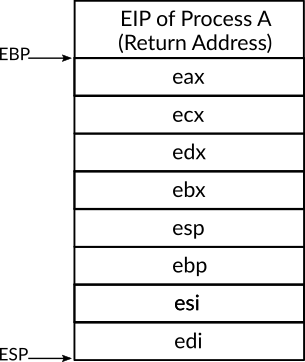
\includegraphics[width=0.35000\textwidth]{Figures/process-ch/Fig21092021_1.png}
\caption{Figure 2: The Stack After Executing the Instruction
\lstinline!pusha!}\label{fig:21092021_1}
\end{figure}
}

Let's assume that a process named \lstinline!A! was running and a system
timer interrupt occurred which caused process \lstinline!A! to suspend
and \lstinline!isr_32! to start, as we have mentioned earlier,
\lstinline!isr_32! will be called as a normal routine and the calling
convention will be followed by the processor. Figure
\protect\hyperlink{fig:21092021_1}{2} shows the stack at the time after
executing \lstinline!pusha! in \lstinline!isr_32!. As you can see, the
context of process \lstinline!A! is on the stack, for example, to reach
the value of \lstinline!ESI! which was stored right before the process
\lstinline!A! has been suspended, we can do that by referring to the
memory address \lstinline!ESP + 4! \footnote{If a new stack frame is
  created once \lstinline!isr_32! starts then also \lstinline!EBP! can
  be used as a base address but with different offset than \lstinline!4!
  of course as we have explained earlier in chapter \ref{ch-x86}. I
  didn't initialize a new stack frame here and in all other places to
  get a shorter code.}, since the current \lstinline!ESP! stores the
memory address of the top of the stack, the size of the value of
\lstinline!EDI! (and all other registers) is \lstinline!4! bytes and the
value of \lstinline!ESI! is next to the top of the stack.

The same technique can be used with any value in stack. As you may have
noticed in the figure, that the return address to where process
\lstinline!A! suspended is stored in the stack, and that's due to the
calling convention which requires the return address of the caller to be
stored in the stack so we can return to it, as you can see, here, the
process \lstinline!A! was considered as the caller and
\lstinline!isr_32! as the callee. So, to obtain the value of process
\lstinline!A!'s return address, we can do that simply by reading the
value in \lstinline!esp + 32!, and that exactly what we have done in the
third step of \lstinline!isr_32! code, we first read this value and then
push it into the stack so the function \lstinline!scheduler! can receive
it as the first parameter.

The fourth and fifth steps are simple, in the fourth step we call the
function \lstinline!scheduler! which we have already discussed, after
the function \lstinline!scheduler! returns, we need to tell PIC that we
finished the handling of an \lstinline!IRQ! by sending end of interrupt
command to the \lstinline!PIC! and that's what is performed in the fifth
step, we have already discussed sending end of interrupt command to PIC
in chapter \ref{ch-progenitor}.

The final thing to do after choosing the next process and performing the
context switching is to give a CPU time for the code of the next
process. This is usually performed by jumping to the memory address in
which the selected process where suspended. There are multiple ways to
do that, the way which we have used in 539kernel is to exploit the
calling convention, again.

As we have mentioned before, the return address to the caller is stored
in the stack, in our previous example, the return address to process
\lstinline!A! was stored in the stack right before the values of process
\lstinline!A! context which have been pushed by the instruction
\lstinline!pusha!. When a routine returns by using the instruction
\lstinline!ret! or \lstinline!iret!, this address will be jumped to, we
exploit this fact to make the next process runs after \lstinline!isr_32!
finishes instead of process \lstinline!A!, this is too simple to be
done, the return address of process \lstinline!A! should be removed from
the stack and in its position in the stack the resume point of the next
process is pushed, that's what we do in the sixth step of
\lstinline!isr_32!.

First we remove all values that we have pushed on the stack while
running \lstinline!isr_32!, this is performed by just adding
\lstinline!40! to the current value of \lstinline!ESP!, we have already
discussed this method of removing values from the stack, why adding
\lstinline!40!? You may ask. The number of values that have been pushed
by the instruction \lstinline!pusha! is \lstinline!8! values, each one
of them of size \lstinline!4! bytes (\lstinline!32-bit!), that means the
total size of them is \lstinline!4 * 8 = 32!. Also, we have pushed the
value of \lstinline!EIP! which also has the size of \lstinline!4! bytes,
so, until now the total size of pushed items in \lstinline!isr_32! is
\lstinline!32 + 4 = 36! and these are all what we have pushed in
purpose, we also need to remove the return address which has been pushed
into the stack before calling \lstinline!isr_32!, the size of memory
addresses in \lstinline!32-bit! architecture is \lstinline!4! bytes
(\lstinline!32-bit!), that means \lstinline!36 + 4 = 40! bytes should be
removed from the stack to ensure that we remove all pushed values with
the return address or process \lstinline!A!.

After that, we simply push the memory address of the function
\lstinline!run_next_process!. In the seventh step, the routine
\lstinline!isr_32! returns indicating that handling an interrupt has
been completed, but instead of returning to the suspended code before
calling the interrupt handler, the code of the function
\lstinline!run_next_process! will be called, which is, as we have seen,
enables the interrupts again and jumps to the resume point of the next
process. In this way, we have got a basic multitasking!

\subsection{Running Processes}\label{running-processes}

In our current environment, we will not be able to test our process
management by using the normal ways, I mean, we can't run a user-space
software to check if its process has been created and being scheduled or
not. Instead, we are going to create a number of processes by creating
their \lstinline!PCB!s via \lstinline!process_create! function, and
their code will be defined as functions in our kernel, the memory
address of these functions will be considered as the starting point of
the process. Our goal of doing that is just to test that our code of
process management is running well. All code of this section will be in
\lstinline!main.c! unless otherwise is mentioned. First, we define
prototypes for four functions, each one of them represents a separate
process, imaging them as a normal use-space software. These prototypes
should be defined before \lstinline!kernel_main!.

\begin{lstlisting}[language=C]
void processA();
void processB();
void processC();
void processD();
\end{lstlisting}

Inside \lstinline!kernel_main!, we define four local variables. Each one
of them represents the PCB of one process.

\begin{lstlisting}[language=C]
    process_t p1, p2, p3, p4;
\end{lstlisting}

Before the infinite loop of \lstinline!kernel_main! we create the four
processes in the system by using the function \lstinline!process_create!
as the following.

\begin{lstlisting}[language=C]
    process_create( &processA, &p1 );
    process_create( &processB, &p2 );
    process_create( &processC, &p3 );
    process_create( &processD, &p4 );
\end{lstlisting}

The code of the processes is the following.

\begin{lstlisting}[language=C]
void processA()
{
    print( "Process A," );

    while ( 1 )
        asm( "mov $5390, %eax" );
}

void processB()
{
    print( "Process B," );

    while ( 1 )
        asm( "mov $5391, %eax" );
}

void processC()
{
    print( "Process C," );

    while ( 1 )
        asm( "mov $5392, %eax" );
}

void processD()
{
    print( "Process D," );

    while ( 1 )
        asm( "mov $5393, %eax" );
}
\end{lstlisting}

Each process starts by printing its name, then, an infinite loop starts
which keeps setting a specific value in the register \lstinline!EAX!. To
check whether multitasking is working fine, we can add the following
lines the beginning of the function \lstinline!scheduler! in
\lstinline!scheduler.c!.

\begin{lstlisting}[language=C]
    print( " EAX = " );
    printi( eax );
\end{lstlisting}

Each time the scheduler starts, it prints the value of \lstinline!EAX!
of the suspended process. When we run the kernel, each process is going
to start by printing its name and before a process starts executing the
value of \lstinline!EAX! of the previous process will be shown.
Therefore, you will see a bunch of following texts
\lstinline!EAX = 5390!, \lstinline!EAX = 5391!, \lstinline!EAX = 5392!
and \lstinline!EAX = 5393! keep showing on the screen which indicates
that the process, \lstinline!A! for example in case
\lstinline!EAX = 5390! is shown, was running and it has been suspended
now to run the next one and so on.

\subsection{\texorpdfstring{Finishing up Version
\texttt{T}}{Finishing up Version T}}\label{finishing-up-version-t}

And we have got version \lstinline!T! of 539kernel which provides us a
basic process management subsystem. The last piece to be presented is
the \lstinline!Makefile! to compile the whole code.

\begin{lstlisting}[language=make]
ASM = nasm
CC = gcc
BOOTSTRAP_FILE = bootstrap.asm 
INIT_KERNEL_FILES = starter.asm
KERNEL_FILES = main.c
KERNEL_FLAGS = -Wall -m32 -c -ffreestanding -fno-asynchronous-unwind-tables -fno-pie
KERNEL_OBJECT = -o kernel.elf

build: $(BOOTSTRAP_FILE) $(KERNEL_FILE)
    $(ASM) -f bin $(BOOTSTRAP_FILE) -o bootstrap.o
    $(ASM) -f elf32 $(INIT_KERNEL_FILES) -o starter.o 
    $(CC) $(KERNEL_FLAGS) $(KERNEL_FILES) $(KERNEL_OBJECT)
    $(CC) $(KERNEL_FLAGS) screen.c -o screen.elf
    $(CC) $(KERNEL_FLAGS) process.c -o process.elf
    $(CC) $(KERNEL_FLAGS) scheduler.c -o scheduler.elf
    ld -melf_i386 -Tlinker.ld starter.o kernel.elf screen.elf process.elf scheduler.elf -o 539kernel.elf
    objcopy -O binary 539kernel.elf 539kernel.bin
    dd if=bootstrap.o of=kernel.img
    dd seek=1 conv=sync if=539kernel.bin of=kernel.img bs=512 count=8
    dd seek=9 conv=sync if=/dev/zero of=kernel.img bs=512 count=2046
    qemu-system-x86_64 -s kernel.img
\end{lstlisting}

Nothing new in here but compiling the new C files that we have added to
539kernel.

    \chapter{Chapter 5: Memory Management}\label{ch-memory-management}

\section{Introduction}\label{introduction}

It's well-known to us right now that one of most important aspects in
modern operating systems is protecting the memory in a way that doesn't
allow a process to access or write to the memory of another process,
furthermore, the memory of the kernel should be protected from the
running processes, that is, they should be prevented from accessing
directly the memory of the kernel or writing to the memory of the
kernel. When we use the term \emph{memory of the kernel} or \emph{memory
of the process}, we mean the region of the main memory that is being
used by the kernel or the process and all of its data or code is stored
in this region of the memory.

In chapter \ref{ch-x86}, we have presented the distinction between the
logical view and physical view of the memory and one of the logical
views of the memory has been presented on the same chapter, this logical
view was segmented-memory model. We have seen how the hardware has
employed the protection techniques to provide memory protection and
protect the segments from each other. In the same chapter, we have
presented another logical view of the memory, it is flat-memory model,
which is exactly same as the physical view of the memory. In this view,
the memory is a big bunch of contiguous bytes and each byte has its
unique address that can be used to refer to this byte in order to read
it or to write to it.

We know that modern operating systems use the flat-memory model and
based on that we decided to use this model on 539kernel instead of the
segmented-memory model. Deciding which model to use is the job of the
kernelist. However, unlike segmentation, when we introduced the
flat-memory model, we haven't shown how the memory can be protected in
it, in this chapter we present one of the methods that can be used to
implement memory protection in flat-memory model. This technique is
known as \emph{paging}, it is a well-known technique that is used widely
by modern operating systems and it has a hardware support in x86
architecture.

\section{Paging in Theory}\label{paging-in-theory}

In paging, the memory of the process (before being loaded to the
physical memory) is divided into a number of fixed size blocks known as
\emph{pages}, in the same manner, the physical memory is divided into
blocks with the same fixed size, these blocks of physical memory are
known as \emph{page frames}. Figure \ref{fig:28092021_0} shows an
example of pages and page frames, as you can see in the figure, process
\lstinline!A! is divided into \lstinline!n! pages and the main memory is
divided into \lstinline!n! page frames, please note that the both
\lstinline!n!s shouldn't necessarily be equal. Because both page and
page frame have the same size, for example \lstinline!4KB! \footnote{That
  is, each page is of size \lstinline!4KB! and each page frame is of
  size \lstinline!4KB!,}, each page can be loaded exactly into one page
frame. To load process \lstinline!A! into the memory, each of its pages
should be loaded into a page frame. A page can be loaded into any page
frame, for example, let's assume we are loading page \lstinline!0! of
process \lstinline!A! and the first free page frame that we found is
page frame \lstinline!30!, then, the page \lstinline!0! can be loaded
into page frame \lstinline!30!. Of course, the pages of more than one
process can be loaded into the page frames.

\begin{figure}
\centering
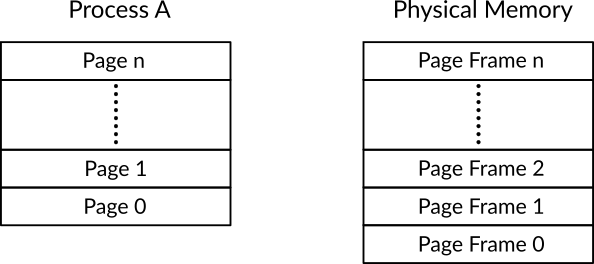
\includegraphics[width=0.35000\textwidth]{Figures/memory-ch/Fig28092021_0.png}
\caption{An Example that Shows Pages and Page
Frames}\label{fig:28092021_0}
\end{figure}

A data structure known as \emph{page table} is used to maintain these
information about the mapping between pages and their corresponding page
frame. Each process has its own page table, in our example of process
\lstinline!A!, the information that tells the processor that page
\lstinline!0! can be found in page frame \lstinline!30! is stored in
process \lstinline!A!'s page table. In paging, any memory address
generated by the process to read or write some data to the memory will
be a logical memory address \footnote{In x86, this logical memory
  address is known as \emph{linear memory address} as we have discussed
  earlier in chapter \ref{ch-x86}.}, that is, a not real not physical
memory address, it has a meaning for the process itself, but for the
processor it should be translated to the corresponding physical memory
address. The page table of the process is used to perform this
translation.

Basically, every generated logical memory address of a process running
in a paging-enabled environment is composed of the following parts: the
page number and the offset. For example, assume a system which employs
paging with length of \lstinline!2! bytes for memory addresses
\footnote{In 32-bit x86 architecture, the length of memory address is
  \lstinline!4 bytes = 32 bits!, that is, \lstinline!2^32 bytes = 4GB!
  are addressable. An example of a memory address in this environment is
  \lstinline!FFFFFFFFh! which is of length \lstinline!4 bytes! and
  refers to the last byte of the memory.}. In this hypothetical system,
the format of logical address is the following, the first byte
represents the page number and the second byte represents the offset.
Process \lstinline!B! is a process that runs in that system, assume that
it performed an instruction to read data from the following memory
address \lstinline!0150h!, this is a logical memory address that needs
to be translated to the physical address to be able to get the required
content. Based on the format of the logical memory addresses in this
system, the first byte of the generated memory address which is
\lstinline!01h! represents the page, that means that the required data
is stored in page \lstinline!01h = 1d! of the process \lstinline!B!, but
where exactly? According the the generated address, it is on the offset
\lstinline!50h = 80d! of that page.

To perform the translation and get the physical memory address, we need
to know in which page frame the page \lstinline!1! of process
\lstinline!B! is loaded. To answer this question the page table of
process \lstinline!B! should be consulted. For each page, there is an
entry in the page table that contains necessary information, and of
course one of those information is the page frame that this page is
stored on. This information can be the page frame number or the base
memory address of the page frame, it doesn't matter since we can get the
base memory address of the page frame by knowing its number and the size
of page frames. After getting the base memory address, we can combine it
with the required offset to get the physical memory address of the data
in question. The hardware that is responsible for the process of memory
address translation is known as \emph{memory management unit} (MMU).

Sometimes, the page table is divided into more than one level. For
example, in two-level page table, the entries of the main page table
refers to an entry on another page table that contains the the base
address of the page frame, x86 architecture uses this design, so we are
going to see it on details later on. The reason of using such design is
the large size of page tables for a large main memory. As you know, the
page table is a data structure that should reside in the main memory
itself, and for each page there is an entry in the page table, in x86
for example, the size of this entry is \lstinline!8! bytes. Furthermore,
the size a page tend to be small, \lstinline!4KB! is a real example of
page size. So, if \lstinline!4GB! is needed to be represented by a page
table with \lstinline!8! bytes of entry size, then \lstinline!8MB! is
needed for this page table which is not a small size for a data
structure needed for each process in the system.

It should be clear by now how paging provides memory protection. Any
memory address that is generated by the process will be translated to
the physical memory by the hardware, there is no way for the process to
access the data of any other process since it knows nothing about the
physical memory and how to reach it. Consider process \lstinline!C! that
runs on the same hypothetical system that we have described above, in
the memory location that's represented by the physical memory address
\lstinline!A1 9Bh! there is some important data which is stored by the
kernel and process \lstinline!C! wishes to read it. If process
\lstinline!C! tries the normal way to read from the memory address
\lstinline!A1 9Bh! the \lstinline!MMU! of the system is going to
consider it as a logical memory address, so, the page table of process
\lstinline!C! is used to identify in which page frame that page
\lstinline!00A1h! of process \lstinline!C! is stored. As you can see,
the process knows nothing about the outside world and cannot gain this
knowledge, it thinks it is the only process in the memory, and any
memory address it generates belongs to itself and it cannot interfere
the translation process or modify its own page table.

\section{Virtual Memory}\label{virtual-memory}

In multitasking system, beside the need of memory protection, also, the
main memory should be utilized as much as we can. In such environment,
multiple processes should reside in the main memory and at some point of
time the main memory will become full and the kernel will not be able to
create any new process before stopping a currently running process to
use its space in the main memory.

There are many situations where the current processes are occupying a
space from the main memory but doesn't really use this space, that
wastes this space since it can be used to load a process that really
needs this space. An example of these situations is when the process is
idle, that is, doing nothing but waiting for some external action
(e.g.~a button click), in this case the only active code of this process
that should be in the main memory is the code that makes the process
waits for an event. Furthermore, modern software tend to be too large,
there are a lot of routines in a code of modern software that might not
be called at all during executing that software, loading the code of
those routines into the main memory wastes the occupied space, the
routines will be there in the memory, taking some space that can be used
for more useful purposes and they will never be called.

Virtual memory is a memory management technique that can be used to
utilize the main memory. You might noticed in modern operating systems,
you can open any number of software in a given time and you never get a
message from the operating system that tells you that there is no enough
space in the main memory although the software that you are running need
a large space of memory (modern web browsers are obvious example), how
can that be achieved? Well, by using virtual memory which depends on
paging that we have discussed earlier.

Regarding to paging, we may ask ourselves an important question, should
all process' pages be loaded into the memory? In fact, not really. As we
have said, the binary code of the software may have a lot of routines
that may not be called, so, the pages that contain these routines should
not be loaded into the memory since they will not be used, instead, this
space can be used for another pages that should really be on the memory.
To realize that, when the software is loaded for the first time, only
the page the contains the entry code of the software (e.g.
\lstinline!main! function in C) is loaded into the memory, not any other
page of that software. When some instruction in the entry code tries to
read data or call a routine that doesn't exist on the loaded page, then,
the needed page will be loaded into the main memory and that piece which
was not there can be used after this loading, that is, any page of the
process will not be loaded into a free page frame unless it's really
needed, otherwise, it will be waiting on the disk, this is known as
\emph{demand paging}.

By employing demand paging, virtual memory saves a lot of memory space.
Furthermore, virtual memory uses the disk for two things, first, to
store the pages that are no demanded yet, they should be there so
anytime one of them is needed, it can be loaded from the disk to the
main memory. Second, the disk is used to implement an operation known as
\emph{swapping}.

Even with demand paging, at some point of time, the main memory will
become full, in this situation, when a page is needed to be loaded the
kernel that implements virtual memory should load it, even if the memory
is full! How? The answer is by using the swapping operation, one of page
frames should be chosen to be removed from the main memory, this frame
in this case is known as \emph{victim frame}, the content of this frame
is written into the disk, it is being \emph{swapped out}, and its place
in the main memory is used for the new page that should be loaded. The
swapped out page is not in the main memory anymore, so, when it is
needed again, it should be reloaded from the disk to the main memory.

The problem of which victim frame should be chosen is known as
\emph{page replacement} problem, that is, when there is no free page
frame and a new page should be loaded, which page frame should we make
free to be able to load the new page. Of course, there are many page
replacement algorithms out there, one of them is \emph{first-in
first-out} in which the page frame that was the first one to be loaded
among the current page frames is chosen as a victim frame. Another
well-known algorithm is \emph{least recently used} (LRU), in this
algorithm, everytime the page is accessed, the time of access is stored,
when a victim frame is needed, then it will be the oldest one that has
been accessed.

The page table can be used to store a bunch of information that are
useful for virtual memory. First, a page table usually has a flag known
as \emph{present}, by using this flag, the processor can tell if the
page that the process tries to access is loaded into the memory or not,
if it is loaded, then a normal access operation is performed, but when
the present flag indicates that this page is not in the memory, what
should be done? For sure, the page should be loaded from the disk to the
memory. Usually, the processor itself doesn't perform this loading
operation, instead, it generates an exception known as \emph{page fault}
and makes the kernel deal with it. A page fault tells the kernel that
one of the processes tried to access a not-loaded page, so it needs to
be loaded. As you can see, page faults help in implementing demand
paging, anytime a page needs to be loaded into the memory then a page
fault will be generated.

With this mechanism that virtual memory uses to manage the memory, we
can make a process to own a size of memory that is not even available on
the system. For example, in x86 architecture with systems that employ
virtual memory, each process thinks that it owns \lstinline!4GB! of main
memory, even if the system has only \lstinline!2GB! of RAM for instance.
This is possible due to demand paging and page replacements. Of course,
a large size of memory being available for the process, makes it easier
for the programmers to write their code.

\section{Paging in x86}\label{paging-in-x86}

In x86, unlike segmentation which is enabled by default, paging is
disabled by default, also, paging is not available on real mode, in
\lstinline!32-bit! environment it can only be used in protected-mode
\footnote{In 64-bit architecture paging is available in both
  protected-mode and long-mode.}. If paging is intended to be used, the
kernel should switch to protected-mode first, then, enables paging
through a special register in x86 known as \lstinline!CR0! which is one
of \emph{control registers} of x86 architecture. The last bit of
\lstinline!CR0! is the one that decides if paging is enabled, when its
value is \lstinline!1!, or disabled when its value is \lstinline!0!.

There are three \emph{paging modes} in x86 a kernelist can chooses from,
the difference between these three modes is basically related to the
size of memory addresses and the available sizes of a page. These modes
are \emph{32-bit paging}, \emph{PAE paging} (PAE stands for ``Physical
Address Extension'') and \emph{4-level paging} which is available for
\lstinline!64-bit! environment only.

Beside the last bit in \lstinline!CR0!, there are another two bits that
can be used to decide the current paging mode. The first one is known as
\emph{PAE bit} which is the fifth bit of the control register
\lstinline!CR4!. When the value of this bit is \lstinline!1! that means
PEA mode is enabled, while \lstinline!0! means otherwise. The second bit
is known as \lstinline!LME! in a register known as
\lstinline!IA32_EFER!, setting the value of this register to
\lstinline!1! makes the processor to switch from the protected-mode
(\lstinline!32-bit! environment) to the long-mode (\lstinline!64-bit!
environment) and when the value of \lstinline!PAE! bit is \lstinline!1!,
then 4-level mode will be enabled.

In our next discussions, we are going to focus on \lstinline!32-bit!
paging mode which is the most basic one that is available for
\lstinline!32-bit! environment. In this mode, there are two available
sizes for a page \lstinline!4KB! and \lstinline!4MB!, also,
\lstinline!4GB! of memory is addressable in this mode.

\subsection{The Structure of Linear Memory
Address}\label{the-structure-of-linear-memory-address}

Previously, we have discussed a part of the translation process of
memory addresses in x86. To sum what we have already discussed up, any
memory address that is generated by an executing code in x86 is known as
a logical address, which is not the real memory address that contains
the required data. This logical address need to be translated to get the
real address. The first step of this translation process is to use
segment descriptors to translate a logical address to a linear address
by using the mechanism that we have already mentioned in chapter
\ref{ch-x86}. When paging is disabled, the resulted linear address will
be the physical (real) address that can be sent to the main memory to
get the required data. On the other hand, when paging is enabled, the
linear address needs a further translation step to obtain the physical
memory address by using paging mechanism. To be able to perform this
step of translation, a page table is used with the parts that compose
the linear address.

\begin{figure}
\centering
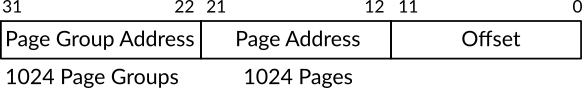
\includegraphics[width=0.35000\textwidth]{Figures/memory-ch/Fig091021_0.png}
\caption{The Structure of Linear Address}\label{fig:10062021_3}
\end{figure}

Figure \ref{fig:10062021_3} shows the structure of a linear address and
its parts. As you can see, the size of a linear address is
\lstinline!32-bit! which is divided into three parts. The bits
\lstinline!22! to \lstinline!31! represent a \emph{page directory}
entry, the bits \lstinline!12! to \lstinline!21! represent a page table
entry and the bits \lstinline!0! to \lstinline!11! represent an offset
that contains the required data within a page frame. For example, assume
a linear address which is composed of the following: page directory
entry \lstinline!x!, page table entry \lstinline!y! and offset
\lstinline!z!. That means that this linear address needs to read the
offset \lstinline!z! from a page that is represented by the entry
\lstinline!y! in the page table, and this page table is represented by
the page directory entry \lstinline!x!.

As you can see here, unlike our previous discussion of page table, the
one which is implemented in x86 is a two-level page table, the first
level is known as \emph{page directory} which is used to point to the
second level which is a page table and each page table, as we know,
points to a page frame. As we mentioned before, the reason of using
multi-level page tables is to save some memory since the size of page
tables tend to have relatively large sizes in modern architecture and
given that each process needs its own page table, then, its better to
use multi-level page table which allows us to load just the needed parts
of a page table (in a way similar to paging) instead of loading the
whole page table into the memory.

\subsection{Page Directory}\label{page-directory}

The page directory in x86 can hold up to \lstinline!1024! entries. Each
entry points to a page table and each one of those page tables can hold
up to \lstinline!1024! entries which represent a process's pages. In
other words, we can say that, for each process, there are more than one
page table, and each one of those page tables is loaded in a different
part of the main memory and the page directory of the process helps us
in locating the page tables of a process.

As we have mentioned before, the page directory is the first level of
x86's page table and each process has its own page directory. How the
processor can find the current page directory, that is, the page
directory of the current process? This can be done by using the register
\lstinline!CR3! which stores the base physical memory address of the
current page directory. The first part of a linear address is an offset
within the page directory, when an addition operation is performed
between the first part of a linear address and the value on
\lstinline!CR3! the result will be the base memory address of the entry
that represents a page table that contains an entry which represents the
page that contains the required data.

\subsubsection{The Structure of a Page Directory
Entry}\label{the-structure-of-a-page-directory-entry}

The size of an entry in the page directory is \lstinline!4! bytes
(\lstinline!32! bits) and its structure is shown in the figure
\ref{fig:10102021_0}. The bits from \lstinline!12! to \lstinline!31!
contain the physical memory address of the page table that this entry
represent. Not all page tables that a page directory points to should be
loaded into the main memory, instead, only the needed page tables, the
rest are stored in a secondary storage until they are needed then they
should be loaded. To be able to implement this mechanism, we need some
place to store a flag that tells us whether the page table in question
is loaded into the main memory or not, and that's exactly the job of bit
\lstinline!0! of a page directory entry, this bit is known as
\emph{present bit}, when its value is \lstinline!1! that means the page
table exists in the main memory, while the value \lstinline!0! means
otherwise. When an executing code tries to read a content from a page
frame that its page table is not in the memory, the processor generates
a page fault that tells the kernel to load this page table because it is
needed right now.

\begin{figure}
\centering
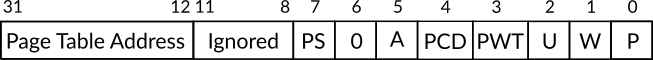
\includegraphics[width=0.35000\textwidth]{Figures/memory-ch/Fig10102021_0.png}
\caption{The Structure of Page Directory Entry}\label{fig:10102021_0}
\end{figure}

When we have discussed segment descriptors, we have witnessed some bits
that aim to provide additional protection for a segment. Paging in x86
also has bits that help in providing additional protection. Bit
\lstinline!1! in a page directory entry decides whether the page table
that the entry points to is read-only when its value is \lstinline!0! or
if its writable \lstinline!1!. Bit \lstinline!2! decides whether the
access to the page table that this entry points to is restricted to
privileged code, that is, the code that runs on privilege level
\lstinline!0!, \lstinline!1! and \lstinline!2! when the bit's value is
\lstinline!0! or that the page table is also accessible by a
non-privileged code, that is, the code that runs on privilege level
\lstinline!3!.

Generally in computing, \emph{caching} is a well-known technique. When
caching is employed in a system, some data are fetched from a source and
stored in a place which is faster to reach if compared to the source,
these stored data are known as \emph{cache}. The goal of caching is to
make a frequently accessed data faster to obtain. Think of your web
browser as an example of caching, when use visit a page \footnote{Please
  do not confuse a web page with a process page in this example.} in a
website, the web browser fetches the images of that page from the source
(the server of the website) and stores it in your own machine's storage
device which is definitely too much faster to access if compared to a
web server, when you visit the same website later, and the web browser
encounters an image to be shown, it searches if it's cached, if so, this
is known as \emph{cache hit}, the image will be obtained from your
storage device instead of the web server, if the image is not cached,
this is known as \emph{cache miss}, the image will be obtained from the
web server to be shown and cached.

The processor is not an exception, it also uses cache to make things
faster. As you may noticed, the entries of page directories and page
tables are frequently accessed, in the code of software a lot of memory
accesses happen and with each memory access both page directory and
pages tables need to be accessed. With this huge number of accesses to
page table and given the fact that the main memory is too much slower
than the processor, then some caching is needed, and that exactly what
is done in x86, a part of the page directory and page tables are cached
in an internal, small and fast memory inside the processor known as
\emph{translation lookaside buffer} (\lstinline!TLB!), each time an
entry of page table of directory is needed, this memory is checked
first, if the needed entry is on it, that is, we got a cache hit, then
it will be used.

In x86 paging, caching is controllable, say that for some reason, you
wish to disable caching for a given entry, that can be done with bit
\lstinline!4! in a page directory entry. When the value of this bit is
\lstinline!1!, then the page table that is represented by this entry
will not be cached by the processor, but the value \lstinline!0! in this
bit means otherwise.

Unlike web browsers, the cached version of page table can be written to,
for example, assume that page table \lstinline!x! has been cached after
using it in the first time and there is a page in this page table, call
it \lstinline!y!, that isn't loaded into the memory. We decided to load
the page \lstinline!y! which means present bit of the entry that
represents this page should be changed in the page table \lstinline!x!.
To make things faster, instead of writing the changes to the page table
\lstinline!x! in the main memory (the source), these changes will be
written to the cache which makes a difference between the cached data
and the source data, that is, they are not identical anymore. This
inconsistency between the two places that store the data should be
resolved somehow, the obvious thing to do is to write these changes
later also on the source.

In caching context, the timing of writing the changes to the source is
known as \emph{write policy} and there are two available policies in x86
for page tables and directory caches, the first one is known as
\emph{write-through}, in this policy, the new data is written on both
the cache and the source at same time. The second policy is known as
\emph{write-back}, in which the writing process is performed only on the
cache, while writing the changes on the source is performed later, for
example when we decide to clear the cache. Bit \lstinline!3! of the page
directory entry decides which write policy will be used for the cached
data, the value \lstinline!1! means write-through policy will be used,
while the value \lstinline!0! means write-back policy will be used.

As in segment descriptors, when a page table which is referred by a
given page directory entry is accessed, there is a bit in the directory
entry known as \emph{access bit} which is the fifth bit in the entry.
The processor sets the value \lstinline!1! automatically when the page
table is accessed. Setting the value to \lstinline!0! for any reason is
the responsibility of the kernel.

We have said earlier that \lstinline!32-bit! paging in x86 provides us
with two possible options for the size of a page, either \lstinline!4KB!
page or \lstinline!4MB! page. The bit \lstinline!7! in a page directory
entry decides the size of the pages, when its value is \lstinline!0!
then the page size will be \lstinline!4KB! while the value \lstinline!1!
means that the page size is \lstinline!4MB!. There is a major difference
between the two options. When the size of the page is \lstinline!4MB!,
the page table will be a normal one-level page table, which means that
the page directory will not refer to a page table anymore, but it is
going to refer to a page frame. When the size of the page is
\lstinline!4KB!, the two-level hierarchy will be employed. That makes
sense, the number of entries that are needed to represent
\lstinline!4KB! pages are way more than the number of entries that are
needed to represent \lstinline!4MB! pages. However, in our discussion,
we have focused (and will focus) on the case of \lstinline!4KB! pages.
Finally, the bits \lstinline!6!, \lstinline!8!, \lstinline!9!,
\lstinline!10! and\lstinline!11! in the page directory entry are
ignored.

\subsection{Page Table}\label{page-table}

In \lstinline!4KB! pages environment, a page table is referred to by an
entry in the page directory. As mentioned earlier, each page table can
hold \lstinline!1024! entries. After finding the base memory address of
the page table in question by consulting the page directory, this base
memory address will be used with the second part of the linear address
to figure out which page table entry should the processor consult to
reach the required data in the physical memory. Of course, the most
important information that a page table entry stores is the base
physical memory address of the page frame, this memory address will be
used with the third part of the linear address (offset) to get the final
physical memory address.

The entry of a page table is exactly same as the entry of a page
directory, its size is \lstinline!4! bytes. Though, there are some
simple differences, the first difference is bit \lstinline!7!, which was
used to decide the page size in page directory, is ignored in the entry
of a page table. The second difference is in bit \lstinline!6!, which
was ignored in the entry of page directory, in page tables this bit is
known as \emph{dirty bit}.

In our previous discussion on virtual memory we know that at some point
of time, a victim frame may be chosen. This frame is removed from the
main memory to free up some space for another page that we need to load
from the disk. When the victim frame is removed from the main memory,
its content should be written to the disk since its content may have
been changed while it was loaded into the memory. Writing the content of
the victim frame to the disk and loading the new page also from disk,
given that the disk is really too slow compared to the processor, is
going to cause some performance penalty.

To make the matter a little bit better, we should write the content of
the victim frame only if there is a real change in its content compared
to the version which is already stored in the disk. If the victim frame
version which is on the main memory and the version on the disk are
identical, there is no need to waste valuable resource on writing the
same content on the disk, for example, page frames that contain only
code will most probably be the same all the time, so their versions on
disk and main memory will be identical. The dirty bit is used to
indicate whether the content of the page frame has been changed and has
differences with the disk version, that is, the page (when the value of
the bit \lstinline!1!) or the two versions are identical (value
\lstinline!0!).

\section{Paging and Dynamic Memory in
539kernel}\label{paging-and-dynamic-memory-in-539kernel}

The last result of this section is version \lstinline!G! of 539kernel
which contains the basic stuff that are related to the memory.
Previously, we have seen that we have no way in 539kernel to allocate
memory dynamically, due to that, the allocation of entries of processes
table and the process control block was a static allocation. Making
dynamic allocation possible is an important thing since a lot of
kernel's objects need to be allocated dynamically. Therefore, the first
memory-related thing to implement is a way to allocate memory
dynamically. The other major part of version \lstinline!G! is
implementing paging by using x86 architecture's support. Since there is
no way yet in 539kernel to access the hard disk, virtual memory cannot
be implemented yet. However, basic paging can be implemented and this
can be used as basis for further development.

\subsection{Dynamic Memory Allocation}\label{dynamic-memory-allocation}

As we have mentioned earlier, in our normal process of developing
applications by using programming languages that don't employ garbage
collection, we are responsible for allocating spaces from memory. When
we need to store data in memory, a free space in memory should be
available for this data to put this data in. The process of telling that
we need \lstinline!n! bytes from memory to store some data is known as
memory allocation. There are two possible ways to allocate memory,
statically or dynamically.

Usually, a static memory allocation is used when we know the size of
data at compile time, that is, before running the application that we
are developing. Dynamic memory allocation is used when the size of data
will be known at run time. Static memory allocation is the
responsibility of the compiler of the language that we are using, while
the dynamic memory allocation is the responsibility of the programmer
\footnote{Not in all cases though.}, also, the regions that we have
allocated dynamically should be freed manually \footnote{This holds true
  in the case of programming languages like C. New system programming
  languages such as Rust for example may have different ways to deal
  with the matter. However, what we are discussing here is the basis,
  depending on this basis more sophisticated concepts (e.g.~Rust) can be
  built.}.

As we have seen, there are multiple region of a running process's memory
and each region has a different purpose, we already discussed run-time
stack which is one of those region. The other data region of a process
that we also discussed previously is the run-time heap. When we allocate
memory dynamically, the memory region that we have allocated is a part
of the run-time heap, which is a large region of process memory that is
used for dynamic allocation, in C, for example, the most well-known way
to allocate bytes dynamically, that is, from the run-time heap is to use
the function \lstinline!malloc! which implements an algorithm known as
\emph{memory allocator}. The run-time heap need to be managed, due to
that, this kind of algorithms use data structures that maintain
information about the allocated space and free space.

A need of dynamic memory allocation have shown up previously in
539kernel. Therefore, in the current version 539kernel we are going to
implement the most basic memory allocator possible. Through a new
function \lstinline!kalloc! (short for \emph{kernel allocate}), which
works in a similar way as \lstinline!malloc!, a bunch of bytes can be
allocate from the kernel's run-time heap, the starting memory address of
this allocated region will be returned by the function, after that, the
region can be used to store whatever we wish. The stuff that are related
to the kernel's run-time heap will be defined in a new file
\lstinline!heap.c! and its header file \lstinline!heap.h!, let's start
with the latter which is the following.

\begin{lstlisting}[language=C]
unsigned int heap_base;

void heap_init();
int kalloc( int );
\end{lstlisting}

A global variable known as \lstinline!heap_base! is defined, this
variable contains the memory address that the kernel's run-time heap
starts from, and starting from this memory address we can allocate
user's needed bytes through the function \lstinline!kalloc! which its
prototype is presented here.

As usual, with each subsystem in 539kernel, there is an initialization
function that sets the proper values and does whatever needed to make
this subsystem ready to use, as you may recall, these functions are
called right after the kernel starts in protected mode, in our current
case \lstinline!heap_init! is the initialization function of the
kernel's run-time heap. We can now start with \lstinline!heap.c!, of
course, the header file \lstinline!heap.h! is needed to be included in
\lstinline!heap.c!, and we begin with the code of \lstinline!heap_init!.

\begin{lstlisting}[language=C]
#include "heap.h"

void heap_init()
{
    heap_base = 0x100000;
}
\end{lstlisting}

As you can see, the function \lstinline!heap_init! is too simple. It
sets the value \lstinline!0x100000! to the global variable
\lstinline!heap_base!. That means that kernel's run-time heap starts
from the memory address \lstinline!0x100000!. In \lstinline!main.c! we
need to call this function in the beginning to make sure that dynamic
memory allocation is ready and usable by any other subsystem, so, we
first add \lstinline!#include "heap.h"! in including section of
\lstinline!main.c!, then we add the call line \lstinline!heap_init();!
in the beginning of \lstinline!kernel_main! function. Next is the code
of \lstinline!kalloc! in \lstinline!heap.c!.

\begin{lstlisting}[language=C]
int kalloc( int bytes )
{
    unsigned int new_object_address = heap_base;
    
    heap_base += bytes;
    
    return new_object_address;
}
\end{lstlisting}

Believe it or not! This is a working memory allocator that can be used
for dynamic memory allocation. It's too simple, though, it has some
disadvantages but in our case it is more than enough. It receives the
number of bytes that the caller needs to allocate from the memory
through a parameter called \lstinline!bytes!.

In the first step of \lstinline!kalloc!, the value of
\lstinline!heap_base! is copied to a local variable named
\lstinline!new_object_address! which represents the starting memory
address of newly allocated bytes, this value will be returned to the
caller so the latter can start to use the allocated memory region
starting from this memory address.

The second step of \lstinline!kalloc! adds the number of allocated bytes
to \lstinline!heap_base!, that means the next time \lstinline!kalloc! is
called, it starts with a new \lstinline!heap_base! that contains a
memory address which is right after the last byte of the memory region
that has been allocated in the previous call. For example, assume we
called \lstinline!kalloc! for the first time with \lstinline!4! as a
parameter, that is, we need to allocate four bytes from kernel's
run-time heap, the base memory address that will be returned is
\lstinline!0x100000!, and since we need to store four bytes, we are
going to store them on the memory address \lstinline!0x100000!,
\lstinline!0x100001!, \lstinline!0x100002! and \lstinline!0x100003!
respectively. Just before returning the base memory address,
\lstinline!kalloc! added \lstinline!4!, which is the number of required
bytes, to the base of the heap \lstinline!heap_base! which initially
contained the value \lstinline!0x100000!, the result is
\lstinline!0x100004! which will be stored in \lstinline!heap_base!. Next
time, when \lstinline!kalloc! is called, the base memory address of the
allocated region will be \lstinline!0x100004! which is, obviously, right
after \lstinline!0x100003!.

As you can see from the allocator's code, there is no way to implement
\lstinline!free! function, usually, this function takes a base memory
address of a region in run-time heap and tells the memory allocator that
the region which starts with this base address is free now and can be
used for other allocations. Freeing memory regions when the code
finishes from using them helps in ensuring that the run-time heap is not
filled too soon, when an application doesn't free up the memory regions
that are not needed anymore, it causes a problem known as \emph{memory
leak}.

In our current memory allocator, the function \lstinline!free! cannot be
implemented because there is no way to know how many bytes to free up
given the base address of a memory region, returning to the previous
example, the region of run-time heap which starts with the base address
\lstinline!0x100000! has the size of \lstinline!4! bytes, if we want to
tell the memory allocator to free this region, it must know what is the
size of this region which is requested to be freed, that of course means
that the memory allocator needs to maintain a data structure that can be
used at least when the user needs to free a region up, one simple way to
be able to implement \lstinline!free! in our current memory allocator is
to modify \lstinline!kalloc! and make it uses, for example, a
linked-list, whenever \lstinline!kalloc! is called to allocate a region,
a new entry is created and inserted into the linked-list, this entry can
be stored right after the newly allocated region and contains the base
address of the region and its size, after that, when the user request to
free up a region by giving its base memory address, the \lstinline!free!
function can search in this linked-list until it finds the entry of that
region and put on the same entry that this region is now free and can be
used for future allocation, that is, the memory which was allocated once
and freed by using \lstinline!free! function, can be used later somehow.

Our current focus is not on implementing a full memory allocator, so, it
is up to you as a kernelist to decide how your kernel's memory allocator
works, of course, there are a bunch of already exist algorithm as we
have mentioned earlier.

\subsubsection{Using The Allocator with Process Control
Block}\label{using-the-allocator-with-process-control-block}

To make sure that our memory allocator works fine, we can use it when a
new process control block is created. It also can be used for processes
table, as you may recall, the processes table from version \lstinline!T!
is an array which is allocated statically and its size is
\lstinline!15!, instead, the memory allocator can be used to implement a
linked-list to store the list of processes. However, for the sake of
simplicity, we will stick here with creating PCB dynamically as an
example of using \lstinline!kalloc!, while keeping the processes table
for you to decide if it should be a dynamic table or not and how to
design it if you decide that it should be dynamic.

The first thing we need to do in order to allocate PCBs dynamically is
to change the parameters list of the function \lstinline!process_create!
in both \lstinline!process.h! and \lstinline!process.c!. As you may
recall, in version \lstinline!T!, the second parameter of this function
called \lstinline!process! and it was the memory address that we will
store the PCB of the new process on it. We had to do that since dynamic
memory allocation wasn't available, so, we were creating local variables
in the caller for each new PCB, then we pass the memory address of the
local variable to \lstinline!process_create! to be used for the new PCB.
This second parameter is not needed anymore since the region of the new
PCB will be allocated dynamically by \lstinline!kalloc! and its memory
address will be returned by the same function. So, the prototype of the
function \lstinline!process_create! will be in \lstinline!process.h! and
\lstinline!process.c! respectively as the following.

\begin{lstlisting}[language=C]
process_t *process_create( int * );
\end{lstlisting}

\begin{lstlisting}[language=C]
process_t *process_create( int *base_address )
\end{lstlisting}

You can also notice that the function now returns a pointer to the newly
created PCB, in version \lstinline!T! it was returning nothing. The next
changes will be in the code of \lstinline!process_create!. The name of
the eliminated parameter of \lstinline!process_create! was
\lstinline!process! and it was a pointer to the type
\lstinline!process_t!. We substitute it with the following line which
should be in the beginning of \lstinline!process_create!.

\begin{lstlisting}[language=C]
process_t *process = kalloc( sizeof( process_t ) );
\end{lstlisting}

Simply, we used the same variable name \lstinline!process! but instead
of getting it as a parameter we define it as a local variable, we call
the memory allocator to allocate a region that has the same size of the
type \lstinline!process_t! from the kernel's run-time heap, exactly as
we do in user-space applications development, so, the new memory region
can be used to store the new PCB and its memory address is stored in the
local variable \lstinline!process!. In the last of
\lstinline!process_create! we should add the line
\lstinline!return process;! to return the memory address for the newly
created PCB for the new process.

In version \lstinline!T! we have called \lstinline!process_create! in
\lstinline!main.c! to create four processes, we need to change the calls
by omitting the second parameter, also the line
\lstinline!process_t p1, p2, p3, p4;! in \lstinline!main.c! which was
allocating memory for the PCBs can be removed since we don't need them
anymore. The calls of \lstinline!process_create! will be as the
following.

\begin{lstlisting}[language=C]
process_create( &processA );
process_create( &processB );
process_create( &processC );
process_create( &processD );
\end{lstlisting}

\subsection{Paging}\label{paging}

In this section we are going to implement a basic paging for 539kernel.
To do that, a number of steps should be performed. A valid page
directory should be initialized and its address should be loaded in the
register \lstinline!CR3!. Also, paging should be enabled by modifying
the value of \lstinline!CR0! to tell the processor to start using paging
and translate linear memory addresses by using the page tables instead
of consider those linear addresses as physical addresses. We have
mentioned earlier, for each process we should define a page table,
however, in this section we are going to define the page table of the
kernel itself since this is the minimum requirement to enable paging.

The page size in 539kernel will be \lstinline!4KB!, that means we need a
page directory that can point to any number of page tables up to
\lstinline!1024! page table. The mapping itself will be \emph{one-to-one
mapping}, that is, each linear address will be translated to a physical
address and both are identical. For example, in one-to-one mapping the
linear address \lstinline!0xA000! refers to the physical address
\lstinline!0xA000!. This choice has been made to make things simple,
more advanced designs can be used instead. We already know the concept
of page frame, when the page size is \lstinline!4KB! that means page
frame \lstinline!0! is the memory region that starts from the memory
address \lstinline!0! to \lstinline!4095d!. One-to-one mapping is
possible, we can simply define the first entry of the first page table
\footnote{The first page table is the one which is pointed to by the
  first entry in the page directory.} to point to page frame
\lstinline!0! and so on. The memory allocator will be used when
initializing the kernel's page directory and page tables, we can
allocate them statically as we have done with \lstinline!GDT! for
example, but that can increase the size of kernel's binary file.

Before getting started with the details two new files are needed to be
created: \lstinline!paging.h! and \lstinline!paging.c! which will
contain the stuff that are related to paging. The content of
\lstinline!paging.h! is the following.

\begin{lstlisting}[language=C]
#define PDE_NUM 3
#define PTE_NUM 1024

extern void load_page_directory();
extern void enable_paging();

unsigned int *page_directory;

void paging_init();
int create_page_entry( int, char, char, char, char, char, char, char, char );
\end{lstlisting}

The part \lstinline!PDE! in the name of the macro \lstinline!PDE_NUM!
means page directory entries, so this macro represents the number of the
entries that will be defined in the kernel's page directory. Any page
directory may hold \lstinline!1024! entries but in our case not all of
these entries are needed so only \lstinline!3! will be defined instead,
that means only three page tables will be defined for the kernel. How
many entries will be defined in those page tables is decided by the
macro \lstinline!PTE_NUM! which \lstinline!PTE! in its name means page
table entries, its value is \lstinline!1024! which means there will be
\lstinline!3! entries in the kernel's page directory and each one of
them points to a page table which has \lstinline!1024! entries. The
total entries will be \lstinline!3 * 1024 = 3072! and we know that each
of these entries map a page frame of the size \lstinline!4KB! then
\lstinline!12MB! of the physical memory will be mapped in the page table
that we are going to define, and since our mapping will be one-to-one,
that means the reachable physical memory addresses start at
\lstinline!0! and ends at \lstinline!12582912!, any region beyond this
range, based on our setting, will not be reachable by the kernel and it
is going to cause a page fault exception. It is your choice to set the
value of \lstinline!PDE_NUM! to the maximum (\lstinline!1024!), this
will make a \lstinline!4GB! of memory addressable.

Getting back to the details of \lstinline!paging.h!, both
\lstinline!load_page_directory! and \lstinline!enable_paging! are
external functions that will be defined in assembly and will be used in
\lstinline!paging.c!. The first function loads the address of the
kernel's page directory in the register \lstinline!CR3!, this address
can be found in the global variable \lstinline!page_directory! but of
course, its value will be available after allocating the needed space by
\lstinline!kalloc!. The second function is the one that modifies the
register \lstinline!CR0! to enable paging in x86, this should be called
after finishing the initialization of kernel's page directory and
loading it.

\subsubsection{Initializing Kernel's Page Directory and
Tables}\label{initializing-kernels-page-directory-and-tables}

From our previous encounter with the structure of page directory/table
entry, we know that the size of this entry is \lstinline!4! bytes and
has a specific arrangement of the bits to indicate the properties of the
entry being pointed to. The function \lstinline!create_page_entry! helps
in constructing a value that can be stored in a page directory/table
entry based on the properties that should be enabled and disabled, this
value will be returned to the caller. As you can see from
\lstinline!paging.h!, it returns an integer and that makes sense, as we
know, the size of integer in \lstinline!32-bit! architecture C is
\lstinline!4! bytes, exactly same as the size of an entry. The following
is the code of \lstinline!create_page_entry! that should be defined in
\lstinline!paging.c!, don't forget to include \lstinline!paging.h!
inside it.

\begin{lstlisting}[language=C]
int create_page_entry( int base_address, char present, char writable, char privilege_level, char cache_enabled, char write_through_cache, char accessed, char page_size, char dirty )
{
    int entry = 0;
    
    entry |= present;
    entry |= writable << 1;
    entry |= privilege_level << 2;
    entry |= write_through_cache << 3;
    entry |= cache_enabled << 4;
    entry |= accessed << 5;
    entry |= dirty << 6;
    entry |= page_size << 7;
    
    return base_address | entry;
}
\end{lstlisting}

As you can see, each parameter of \lstinline!create_page_entry!
represents a field in the entry of page directory/table, the possible
values of all of them but \lstinline!base_address! are either
\lstinline!0! or \lstinline!1!, the meaning of each value depends on the
flag itself and we already have covered them. By using bitwise
operations we put each flag in its correct place.

The base address represents the base memory address of a page table in
case we are creating a page directory entry, while it represents the
base memory address of a page frame in case we are creating a page table
entry. This base address will be \lstinline!OR!red with the value that
is generated to represent the properties of the entity that the current
entry is pointing to, we will discuss more details about the base memory
address when we start talking about page-aligned entries.

Now we can use \lstinline!create_page_entry! to implement the function
\lstinline!paging_init! which should reside in \lstinline!paging.c!.
This function will be called when the kernel switches to protected-mode,
as the usual with initialization functions, its job is creating the
kernel's page directory and kernel's page tables that implement
one-to-one map based on the sizes that defined in the macros
\lstinline!PDE_NUM! and \lstinline!PTE_NUM!. The code of
\lstinline!paging_init! is the following.

\begin{lstlisting}[language=C]
void paging_init()
{
    // PART 1:
    
    unsigned int curr_page_frame = 0;
    
    page_directory = kalloc( 4 * 1024 );
        
    for ( int currPDE = 0; currPDE < PDE_NUM; currPDE++ )
    {
        unsigned int *pagetable = kalloc( 4 * PTE_NUM );
        
        for ( int currPTE = 0; currPTE < PTE_NUM; currPTE++, curr_page_frame++ )
            pagetable[ currPTE ] = create_page_entry( curr_page_frame * 4096, 1, 0, 0, 1, 1, 0, 0, 0 );
        
        page_directory[ currPDE ] = create_page_entry( pagetable, 1, 0, 0, 1, 1, 0, 0, 0 );
    }
    
    // ... //
    
    // PART 2
    
    load_page_directory();
    enable_paging();
}
\end{lstlisting}

For the sake of simpler discussion, I have divided the code of the
function into two parts and each part is indicated by a heading comment.
The job of the first part is to create the page directory and the page
tables. Based on the default values of \lstinline!PDE_NUM! and
\lstinline!PTE_NUM!, three entries will be defined in the page
directory, each one of them points to a page table that contains
\lstinline!1024! entries.

First, we allocate \lstinline!4 * 1024! from the kernel's heap for the
page directory, that's because the size of each entry is \lstinline!4!
bytes, as you can see, while we need only three entries for the page
directory, we are allocating memory for \lstinline!1024! entries
instead, the reason of that is the following: the base memory address of
a page table should be page-aligned, also, the base memory address of a
page frame should be page-aligned. When the page size is
\lstinline!4KB!, then a memory address that we can describe as a
\emph{page-aligned memory address} is the one that is a multiple of
\lstinline!4KB!, that is, a multiple of \lstinline!4096!. In other
words, it should be dividable by \lstinline!4096! with no remainder. The
first six multiples of \lstinline!4KB! are \lstinline!0 = 4096 * 0!,
\lstinline!4096 = 4096 * 1!, \lstinline!8192 = 4096 * 2!
(\lstinline!8KB!), \lstinline!12288 = 4096 * 3! (\lstinline!12KB!),
\lstinline!16384 = 4096 * 4! (\lstinline!16KB!),
\lstinline!20480 = 4096 * 5! (\lstinline!20KB!) and so on. Each one of
those value can be considered as a page-aligned memory address when the
page size is \lstinline!4KB!.

Let's get back to the reason of allocating \lstinline!4 * 1024! bytes
for the page directory instead of \lstinline!4 * 3! bytes. We know that
memory allocator sets the base of the heap from the memory address
\lstinline!0x100000!, also, we know, based on the code order of the
kernel that \lstinline!paging_init! will be the first code ever that
calls \lstinline!kalloc!, that is, \lstinline!kalloc! will be called the
first time in 539kernel when we allocate a region for kernel's page
directory in the line \lstinline!page_directory = kalloc( 4 * 1024 );!
which means that the memory address of kernel's page directory will be
\lstinline!0x100000! (\lstinline!1048576d!) which is a page-aligned
memory address since \lstinline!1048576 / 4096 = 256! (in hexadecimal:
0x100000 / 0x1000 = 0x100) with no remainders.

When we allocate \lstinline!4 * 1024! bytes for the page directory (the
first case), the next memory address that will be used by the memory
allocator for the next allocation will be
\lstinline!1048576 + ( 4 * 1024 ) = 1052672! (\lstinline!0x101000!)
which is also a page-aligned memory address. The second case is when we
allocate \lstinline!4 * 3! bytes for the page directory instead, the
next memory address that the memory allocator will use for the next
allocation will be \lstinline!1048576 + ( 4 * 3 ) = 1048588!
(\lstinline!0x10000C!) which is not a page-aligned memory address and
cannot be used as a base memory address for a page table.

If you continue reading the function \lstinline!paging_init! you will
see that the next thing that will be allocated via \lstinline!kalloc!
after that page directory is the first page table which should be in a
page-aligned memory address, due to that, we have used the first case
which ensures that the next call of \lstinline!kalloc! is going to
return a page-aligned memory address instead of the second case which
will not, of course, this is a quick and dirty solution.

Getting back to the first part of \lstinline!paging_init!, as you can
see, it is too simple, it allocates regions from the kernel's heap for
the page directory and the entries of the three page tables. Then each
entry in both page table and page directory is being filled by using the
function \lstinline!create_page_entry!. Let's start with the line which
defines entries in a page table.

\begin{lstlisting}[language=C]
create_page_entry( curr_page_frame * 4096, 1, 0, 0, 1, 1, 0, 0, 0 )
\end{lstlisting}

Given that the size of a page is \lstinline!4KB!, then, page frame
number \lstinline!0! which is the first page frame starts at the
physical memory address \lstinline!0! and ends at physical memory
address \lstinline!4095!, in the same way, page frame \lstinline!1!
starts at the physical memory address \lstinline!4096! and ends at the
physical memory address \lstinline!8191! and so on. In general, with
one-to-one mapping, given \lstinline!n! is the number of a page frame
and the page size is \lstinline!4KB!, then \lstinline!n * 4096! is the
physical memory address that this page frame starts at. We use this
equation in the first parameter that we pass to
\lstinline!create_page_entry! when we create the entries that point to
the page frames, that is, page tables entries. The local variable
\lstinline!curr_page_frame! denotes the current page frame that we are
defining an entry for, and this variable is increased by \lstinline!1!
with each new page table entry. In this way we can ensure that the page
tables that we are defining use a one-to-one map.

As you can see from the rest of the parameters, for each entry in the
page table, we set that the page frame is present, its cache is enabled
and write-through policy is used. Also, the page frame belongs to
supervisor privilege level and the page size is \lstinline!4KB!.

The code which define a new entry in the page directory is similar to
the one which define an entry in a page table, the main difference is,
of course, the base address which should be the memory address of the
page table that belongs to the current entry of the page directory. When
we allocate a memory region for the current page table that we are
defining, its base memory address will be returned by \lstinline!kalloc!
and stored in the local variable \lstinline!pagetable! which is used as
the first parameter when we define an entry in the page directory.

\paragraph{The Need of Page-aligned Memory
Addresses}\label{the-need-of-page-aligned-memory-addresses}

In the previous section we have discussed the meaning of a page-aligned
memory address, and we stated the fact that any base memory address that
is defined in a page directory/table entry should be a page-aligned
memory address. Why? You may ask.

Recalling the structure of page directory/table entry, it is known that
the number of bits that are dedicated for the base memory address are
\lstinline!20! bits (\lstinline!2.5! bytes or \lstinline!2! bytes and a
nibble), also, we know that in \lstinline!32-bit! architecture, the size
of the largest memory address (\lstinline!0xFFFFFFFF!) is of size
\lstinline!32! bits.

Now, assume that we want to define a page table entry that points to the
last possible page frame which its base address is
\lstinline!0xFFFFF000!. To store this full address \lstinline!32! bits
are needed \footnote{Remember, each hexadecimal digit represents a
  nibble. One byte consists of two nibbles.} but only \lstinline!20!
bits are available for base memory address in the page table entry, so,
how can we point to this page frame since we can't store its full
address in the entry?

The numbers that we have defined previously as page-aligned numbers, in
other words, the multiples of \lstinline!4096!, have an interesting
property when they are represented in hexadecimal format, they always
end with three zeros! \footnote{And that makes sense, the first one of
  them after zero is \lstinline!0x1000! (\lstinline!4096d!) and to get
  the next one you need to add \lstinline!0x1000! on the previous one
  and so on.} In our current example of the last possible page frame, we
need to store \lstinline!0xFFFFF000! as a base memory address, you can
see that it ends with three zeros which means that this number is a
page-aligned number. Removing the last three zeros of the example memory
address gives us the value \lstinline!0xFFFFF! which exactly needs
\lstinline!20! bits to be stored, so, due to that the base address the
is stored in page directory/table should be a page-aligned memory
address which makes it possible to remove the last three zeros from it
and make its size \lstinline!20! bits and later on the processor will be
able to get the correct full base address from the \lstinline!20!bits in
the entry, simply, by appending three zeros to it. In
\lstinline!create_page_entry! the place of these three zeros were used
to store the properties of the entry when we \lstinline!OR!red the base
address with the value that has been constructed to represent the
properties.

\subsubsection{Loading Kernel's Page Directory and Enabling
Paging}\label{loading-kernels-page-directory-and-enabling-paging}

The second part of the function \lstinline!paging_init! performs two
operations, the first one is loading the content of the global variable
\lstinline!page_directory! in the register \lstinline!CR3!, that is,
loading the kernel's page directory so that the processor can use it
when the second operation, which enables the paging, is performed.

Because both of these functions need to access the registers directly,
they will be written in assembly in the file \lstinline!starter.asm!.
Till now, it is the first time that we define a function in assembly and
use it in C code, to do that we need to add the following lines in the
beginning of \lstinline!starter.asm! after
\lstinline!extern run_next_process!.

\begin{lstlisting}
extern page_directory

global load_page_directory
global enable_paging
\end{lstlisting}

There is nothing new in the first line. We are telling NASM that there
is a symbol named \lstinline!page_directory! that will be used in the
assembly code, but it isn't defined in it, instead it's defined in a
place that the linker is going to tell you about in the future. As you
know, \lstinline!page_directory! is the global variable that we have
defined in \lstinline!paging.h! and holds the memory address of the
kernel's page directory, it will be used in the code of
\lstinline!load_page_directory!.

The last two lines are new, what we are telling NASM here is that there
will be two labels in current assemble code named
\lstinline!load_page_directory! and \lstinline!enable_paging!, both of
them should be global, that is, they should be reachable by places other
than the current assembly code, in our case, it's the C code of the
kernel. The following is the code of those functions, they reside in
\lstinline!starter.asm! below the line \lstinline!bits 32! since they
are going to run in \lstinline!32-bit! environment.

\begin{lstlisting}
load_page_directory:
    mov eax, [page_directory]
    mov cr3, eax
    
    ret
    
enable_paging:
    mov eax, cr0
    or eax, 80000000h
    mov cr0, eax
    
    ret
\end{lstlisting}

There is nothing new here. In the first function we load the content of
\lstinline!page_directory! into the register \lstinline!CR3! and in the
second function we use bitwise operation to modify bit \lstinline!31! in
\lstinline!CR0! and sets its value to \lstinline!1! which means enable
paging. Finally, \lstinline!paging_init! should be called by
\lstinline!kernel_main! right after \lstinline!heap_init!, the full list
of calls in the proper order is the following.

\begin{lstlisting}[language=C]
heap_init();
paging_init();  
screen_init();
process_init();
scheduler_init();
\end{lstlisting}

\subsection{\texorpdfstring{Finishing up Version
\texttt{G}}{Finishing up Version G}}\label{finishing-up-version-g}

And now version \lstinline!G! of 539kernel is ready. It contains a basic
memory allocator and a basic paging. The following is its
\lstinline!Makefile! which adds the new files to the compilation list.

\begin{lstlisting}[language=make]
ASM = nasm
CC = gcc
BOOTSTRAP_FILE = bootstrap.asm 
SIMPLE_KERNEL = simple_kernel.asm
INIT_KERNEL_FILES = starter.asm
KERNEL_FILES = main.c
KERNEL_FLAGS = -Wall -m32 -c -ffreestanding -fno-asynchronous-unwind-tables -fno-pie
KERNEL_OBJECT = -o kernel.elf

build: $(BOOTSTRAP_FILE) $(KERNEL_FILE)
    $(ASM) -f bin $(BOOTSTRAP_FILE) -o bootstrap.o
    $(ASM) -f elf32 $(INIT_KERNEL_FILES) -o starter.o 
    $(CC) $(KERNEL_FLAGS) $(KERNEL_FILES) $(KERNEL_OBJECT)
    $(CC) $(KERNEL_FLAGS) screen.c -o screen.elf
    $(CC) $(KERNEL_FLAGS) process.c -o process.elf
    $(CC) $(KERNEL_FLAGS) scheduler.c -o scheduler.elf
    $(CC) $(KERNEL_FLAGS) heap.c -o heap.elf
    $(CC) $(KERNEL_FLAGS) paging.c -o paging.elf
    ld -melf_i386 -Tlinker.ld starter.o kernel.elf screen.elf process.elf scheduler.elf heap.elf paging.elf -o 539kernel.elf
    objcopy -O binary 539kernel.elf 539kernel.bin
    dd if=bootstrap.o of=kernel.img
    dd seek=1 conv=sync if=539kernel.bin of=kernel.img bs=512 count=8
    dd seek=9 conv=sync if=/dev/zero of=kernel.img bs=512 count=2046
    qemu-system-x86_64 -s kernel.img
\end{lstlisting}


    \chapter{Chapter 6: Filesystems}\label{ch-filesystems}

\section{Introduction}\label{introduction}

Given that both the processor and the main memory are resources in the
system, till this point, we have seen how a kernel of an operating
system works as a resource manager, 539kernel manages these resources
\footnote{Incompletely of course, to keep 539kernel as simple as
  possible, only the basic parts of resources management were presented.}
and provides them to the different processes in the system.

Another role of a kernel is to provide a way to communicate with
external devices, such as the keyboard and hard disk. \emph{Device
drivers} are the way of realizing this role of the kernel. The details
of the external devices and how to communicate with them are low-level
and may be changed at any time. The goal of a device driver is to
communicate with a given device by using the device's own
language\footnote{The word \emph{language} here is a metaphor, it
  doesn't mean a programming language.} in behalf of any component of
the system (e.g.~a process) that would like to use the device. Device
drivers provide an interface so it can be called by the other system's
components in order to tell the device something to do, we can consider
this interface as a library that we use in normal software development.
In this way, the low-level details of the device is hidden from the
other components and whenever these details changed only the code of the
device driver should be changed, the interface can be kept to not affect
its users. Also, hiding the low-level details from driver's user can
ensure the simplicity of using that driver.

The matter of hiding the low-level details with something higher-level
is too important and can be found, basically, everywhere in computing
and the kernels are not an exception of that. Of course, there is
virtually no limit of providing higher-level concepts based on a
previous lower-level concept, also, upon something that we consider as a
high-level concept we can build something even higher-level. Beside the
previous example of device drivers, one of obvious examples where the
kernels fulfill the role of hiding the low-level details and providing
something higher-level, in other words, providing an \emph{abstraction},
is a filesystem which provides the well-known abstraction, a file.

In this chapter we are going to cover these two topics, device drivers
and filesystem by using 539kernel. As you may recall, it turned out that
accessing to the hard disk is an important aspect for virtual memory,
so, to be able to implement virtual memory, the kernel itself needs to
access the hard disk which makes it an important component in the
kernel, so, we are going to implement a device driver that communicate
with the hard disk in this chapter. After getting the ability of reading
from the hard disk or writing to it, we can explore the idea of
providing abstractions by the kernel through writing a filesystem that
uses the hard disk device driver and provides a higher-level view of the
hard disk that we all familiar with instead of the physical view of the
hard disk which has been described previously in chapter
\ref{ch-bootloader}. The final result of this chapter is version
\lstinline!NE! of 539kernel.

\section{ATA Device Driver}\label{ata-device-driver}

No need to say the hard disks are too common devices that are used as
secondary storage devices. There are a lot of manufacturers that
manufacture hard disks and sell them, imagine for a moment that each
hard disk from a different manufacturer use its own way for the
communication between the software and the hard disk, that is, the
method \lstinline!X! should be used to be able to communicate with hard
disks from manufacturer \lstinline!A! while the method \lstinline!Y!
should be used with hard disks from manufacturer \lstinline!B! and so
on, given that there are too many manufacturers, this will be a
nightmare. Each hard disk will need its own device driver which talks a
different language from the other hard disk device drivers.

Fortunately, this is not the case, at least for the hard disks, in these
situations, standards are here to the rescue. A manufacturer may design
the hard disk hardware in anyway, but when it comes to the part of the
communication between the hard disk and the outside world, a standard
can be used, so, any device driver that works with this given standard
will be able to communicate with this new hard disk. There are many
well-known standards that are related to the hard disks, \emph{small
computer system interface} (SCSI) is one of them, another one is
\emph{advanced technology attachment} (ATA), another well-known name for
ATA is \emph{Integrated Drive Electronics} (IDE). The older ATA standard
is now known as Parallel ATA (PATA) while the newer version of ATA is
known as Serial ATA (SATA). Because ATA is more common in personal
computers we are going to focus on it here and write a device driver for
it, SCSI is more common in servers.

As in PIC which has been discussed in chapter \ref{ch-progenitor}, ATA
hard disks can be communicated with by using port-mapped I/O
communication through the instructions \lstinline!in! and
\lstinline!out!. But before discussing the ATA commands that let us to
issue a read or write request to the hard disk, let's write two routines
in assembly that can be used used as C functions in C code and perform
the same functionality of the instructions \lstinline!in! and
\lstinline!out!.

If you don't recall, the instruction \lstinline!out! is used to write
some bytes on a given port number, so, if we know the port number that a
device (e.g.~hard disk) receives commands from, we can use the
instruction \lstinline!out! to write a valid command to that port. On
the other hand, the instruction \lstinline!in! reads data from a given
port, for example, sometimes after we send a command to a device, it
responds by writing something on a specific port, the instruction
\lstinline!in! can be used to read this value.

The assembly code of the both routines that we are going to define next
should reside in \lstinline!starter.asm! anywhere between
\lstinline!bits 32! and the beginning of \lstinline!start_kernel!
routine. The following is the code of \lstinline!dev_write! which can be
used by C kernel code to write to a given port. In C, we can see that it
has this prototype: \lstinline!dev_write( int port, int cmd )!.

\begin{lstlisting}
dev_write:
    ; Part 1
    push edx
    push eax
    
    ; Part 2
    xor edx, edx
    xor eax, eax
    
    ; Part 3
    mov dx, [esp + 12]
    mov al, [esp + 16]
    
    ; Part 4
    out dx, al 
    
    ; Part 5
    pop eax
    pop edx
    
    ret
\end{lstlisting}

The core part of this routine is part four which contains the
instruction \lstinline!out! that sends the value of \lstinline!AL! to
the port number which is stored in \lstinline!DX!. Because we are using
these two registers \footnote{Which are, as you know, parts of the
  registers \lstinline!EAX! and \lstinline!EDX! respectively.}, we push
their previous values into the stack and that's performed in the first
part of the routine. Pushing the previous values of these registers lets
us restore them easily after the routine finishes its work, this
restoration is performed in the fifth part of the routine right before
returning from it, this is an important step to make sure that when the
routine returns, the environment of the caller will be same as the one
before calling the routine.

After storing the previous values of \lstinline!EAX! and \lstinline!EDX!
we can use them freely, so, the first step after that is to clear their
previous values by setting the value \lstinline!0! to the both of them,
as you can see, we have used \lstinline!xor! and the both operands of it
are the same register (hence, value) that we wish to clear, this is a
well-known way in assembly programming to clear the value of a register
\footnote{To my best knowledge its performance is better than the normal
  way of using \lstinline!mov!.}. After that, we can move the values
that have been passed to the routine as parameters to the correct
registers to be used with \lstinline!out! instruction, this is performed
in the third part of the routine \footnote{You may notice that I've
  omitted the epilogue of routines that creates a new stack frame, this
  decision has been made to make the matters simpler and shorter, you
  are absolutely free to use the calling convention and most probably
  using it is a better practice.}.

Beside \lstinline!dev_write!, we need to define another routine called
\lstinline!dev_write_word! which is exactly same as
\lstinline!dev_write! but write a word (\lstinline!2! bytes) instead of
one byte to a port. The following is the code of this routine.

\begin{lstlisting}
dev_write_word:
    push edx
    push eax    
    
    xor edx, edx
    xor eax, eax
    
    mov dx, [esp + 12]
    mov ax, [esp + 16]
    
    out dx, ax 
    
    pop eax
    pop edx
    
    ret
\end{lstlisting}

As you can see, the only difference between \lstinline!dev_write! and
\lstinline!dev_write_word! is that the first one uses the register
\lstinline!al! (\lstinline!8! bit) as the second operand of
\lstinline!out! while the second one uses \lstinline!ax! (\lstinline!16!
bit) instead, so, a word can be written to the port.

The following is the code of the routine \lstinline!dev_read! which uses
the instruction \lstinline!in! to read the data from a given port and
returns them to the caller, its prototype can be imagined as
\lstinline!char dev_read( int port )!.

\begin{lstlisting}
dev_read:
    push edx
    
    xor edx, edx
    xor eax, eax
    
    mov dx, [esp + 8]
    
    in ax, dx
    
    pop edx
    
    ret
\end{lstlisting}

For the same reason of restoring the previous environment when returning
to the caller, the routine pushes the value of \lstinline!edx! into the
stack, then both of \lstinline!EDX! and \lstinline!EAX! are cleared
since they will be used by the instruction \lstinline!in!. After that,
the value of the passed parameter which represents the port number that
caller wishes to read from, is stored in \lstinline!DX!. Finally,
\lstinline!in! is called, the result is stored in \lstinline!AX!, since
the first operand of \lstinline!in! is \lstinline!AX! and not
\lstinline!AL! then a \textbf{word} will be read from the port and not a
single byte. The decision of using \lstinline!AX! instead of
\lstinline!AL! was made here because of our needs as you will see later,
if you need to read just one byte for some reason you can define another
routine for that. Finally, the previous value of \lstinline!EDX! is
restored and the routine returns.

You may ask, why did we only store and restore the previous value of
\lstinline!EDX! and not \lstinline!EAX! which was also used in the code
of the routine? The reason is that \lstinline!dev_read! is a function
that returns a value, and according to the calling convention the
returned value from a function should be stored in the register in
\lstinline!EAX!, so, the value of \lstinline!EAX! is intended to be
changed when return to the caller, therefore, it will not be correct,
logically, to restore the the previous value of \lstinline!WAX! when
\lstinline!dev_read! returns.

Because the ultimate goal of defining both \lstinline!dev_write! and
\lstinline!dev_read! is to make them available to be used in C code, so,
the lines \lstinline!global dev_write!,
\lstinline!global dev_write_word! and \lstinline!global dev_read! should
be written in the beginning of \lstinline!starter.asm! after
\lstinline!global enable_paging!.

\subsection{The Driver}\label{the-driver}

One ATA bus in the computer's motherboard makes it possible to attach
two hard disks into the system, one of them is called master drive which
is the main one that the computer boots from, the other disk is known as
slave drive. Usually, a computer comes with two ATA buses instead of
just one, which means up to four hard disks can be attached into the
computer. The first one of those buses is known as the primary bus while
the second one is known as the secondary bus.

Terms that combine a bus name with a device name are used to specify
exactly which device is being discussed, for example, primary master
means the master hard disk that is connected to the primary bus while
secondary slave means the slave hard disk which is connected to the
secondary bus.

The port numbers that can be used to communicate with the devices that
are attached into the primary bus start from \lstinline!0x1F0! and ends
in \lstinline!0x1F7! each one of these ports has its own functionality.
The port numbers from \lstinline!0x170! to \lstinline!0x177! are used to
communicate with devices that are attached into the secondary bus, so,
there are eight ports for each ATA bus.

For the sake of simplicity, our device driver is going to assume that
there is only a primary master and all read and write requests should be
sent to this primary master, therefore, our device driver uses the port
number \lstinline!0x1F0! as the base port to send the commands via PIC.

You may ask, why are we calling this port number a base port? As you
know that all the following port numbers are valid to communicate with
the primary ATA bus: \lstinline!0x1F0!, \lstinline!0x1F1!,
\lstinline!0x1F2!, \lstinline!0x1F3!, \lstinline!0x1F4!,
\lstinline!0x1F5!, \lstinline!0x1F6!, \lstinline!0x1F7!, so, we can add
any number from \lstinline!0! through \lstinline!7! to the base port
number of the primary bus \lstinline!0x1F0! to get a correct port
number, the same holds true with the secondary ATA bus which its base
port number is \lstinline!0x170!. So, we can define the base port as a
macro (or even variable) as we will see in our device driver, then we
can use this macro by adding a specific value to it from \lstinline!0!
through \lstinline!7! to get a specific port, the advantage of doing so
is the easiness of changing the value of the base port to another port
without the need of changing the code itself.

Before starting in the implementation of the driver, let's create two
new files: \lstinline!ata.h! and \lstinline!ata.c! which will contain
the code of the ATA device driver which provides an interface for the
rest of the kernel to write to and read from the disk. The following is
the content of \lstinline!ata.h! and the details of the functions will
be discussed in the next subsections.

\begin{lstlisting}[language=C]
#define BASE_PORT 0x1F0
#define SECTOR_SIZE 512

void wait_drive_until_ready();

void *read_disk( int );
void write_disk( int, short * );

void *read_disk_chs( int );
void write_disk_chs( int, short * );
\end{lstlisting}

\subsubsection{Addressing Mode}\label{addressing-mode}

As in the main memory, the hard disks use addresses to read the data
that are stored in a specific area of the disk, the same is applicable
in write operation, the same address can be used to write on the same
specific area. There are two schemes of hard disk addresses, the older
one is known as \emph{cylinder-head-sector} addressing (\lstinline!CHS!)
while the newer one which more dominant now is known as \emph{logical
block addressing} (\lstinline!LBA!).

In chapter \ref{ch-bootloader} we have covered the physical structure of
hard disks and we know from that discussion that the data are stored in
small blocks known as sectors, also, there are tracks which each one of
them consists of a number of sectors, and finally, there are heads that
should be positioned on a specific sector to read from it or to write to
it. The scheme \lstinline!CHS! uses the same concepts of physical
structure of hard disk, the address of a given sector on the hard disk
should be composed by combining three numbers together, the cylinder
(track) that this sector reside on, the sector that we would like to
access and the head that is able to access this sector. However, this
scheme is obsolete now and \lstinline!LBA! is used instead of it.

In \lstinline!LBA!, a logical view of a hard disk is used instead of the
physical view. This logical view states that the hard disk is composed
of a number of logical blocks with a fixed size, say, \emph{n} bytes.
These blocks are contagious in a similar way of the main memory and to
reach any block you can use its own address, the addresses start from
\lstinline!0!, the block right after the first one has the address
\lstinline!1! and so on. As you can see, addressing in \lstinline!LBA!
is more like the addressing of the main memory, the main difference here
is that in current computers each address of the main memory points to a
byte in memory while an address in \lstinline!LBA! points to a block
which can be a sector (\lstinline!512! bytes) or even bigger.

\subsubsection{Reading from Disk}\label{reading-from-disk}

In this subsection we are going to implement both
\lstinline!read_disk_chs! and \lstinline!read_disk! which send commands
to an ATA hard disk via the available ports in order to read a
sector/block from the disk. The first one of those functions uses
\lstinline!CHS! scheme while the second one uses \lstinline!LBA! scheme.
In the next discussions, I'm going to use the symbol
\lstinline!base_port! to indicate the base port of one of ATA ports, in
our case, the base port is \lstinline!0x1F0! since we are going to use
the primary bus in our device driver, but what we are discussing is
applicable to any ATA bus with any base port number.

To issue a read command the value \lstinline!0x20! should be sent to
\lstinline!base_port + 7!, but before doing that, a number of values
should be set in the other ports in order to specify the address that we
would like to read from. These ports are the following: In
\lstinline!base_port + 2! the number of sectors/blocks that we would
like to read in this operation should be set.

The value that should be written to \lstinline!base_port + 6! specifies
more than one thing, bit \lstinline!6! of this value specifies whether
we are using \lstinline!CHS! or \lstinline!LBA! in the current read
request, when the bit's value is \lstinline!0! then \lstinline!CHS! is
being used while the value \lstinline!1! means that \lstinline!LBA! is
being used. The bits \lstinline!5! and \lstinline!7! of this value
should always be \lstinline!1!. The bit \lstinline!4! is used to specify
the drive that we would like to read from, the value \lstinline!0! for
the master drive while \lstinline!1! for the slave drive. In the case
that we are using \lstinline!CHS!, then the first four bits
(\lstinline!0! to \lstinline!3!) of this value is used to specify the
head while in the case that we are using \lstinline!LBA!, these bits
store a part from the \lstinline!LBA! address, this part starts from bit
\lstinline!24! to bit \lstinline!27!.

When the current addressing mode is \lstinline!CHS!, the sector number
that we would like our read operation to start from should be sent to
\lstinline!base_port + 3!, the low part of the cylinder number should be
sent to \lstinline!base_port + 4! and the high part of the cylinder
number should be sent to \lstinline!base_port + 5!. The following table
summarizes the parameters to the read command when the addressing mode
is \lstinline!CHS!.

\begin{longtable}[]{@{}ll@{}}
\toprule
Port Number & Purpose (in CHS)\tabularnewline
\midrule
\endhead
base\_port + 2 & Number of Sectors to Read\tabularnewline
base\_port + 3 & The Sector Number to Read From\tabularnewline
base\_port + 4 & Lower Part of the Cylinder Number\tabularnewline
base\_port + 5 & Higher Part of the Cylinder Number\tabularnewline
base\_port + 7 & Command Port. Read Command: 0x20\tabularnewline
\bottomrule
\end{longtable}

\begin{longtable}[]{@{}lll@{}}
\toprule
Port Number & Bit(s) & Purpose (in CHS)\tabularnewline
\midrule
\endhead
base\_port + 6 & 0-3 & The Head\tabularnewline
& 4 & Drive to Use (0 = Master, 1 = Slave)\tabularnewline
& 5 & Always 1\tabularnewline
& 6 & Addressing Mode (0 for CHS)\tabularnewline
& 7 & Always 1\tabularnewline
\bottomrule
\end{longtable}

Once the read command is issued with the right parameters passed to the
correct ports, we can read the value of \lstinline!base_port + 7! to
check if the disk finished the reading operating or not by reading the
eighth bit (bit \lstinline!7!) of that value, when the value of this bit
is \lstinline!1! that means the drive is busy, once it becomes
\lstinline!0! that means that the operation completed.

When the reading operation is completed successfully, the data are
brought to \lstinline!base_port! which means we need to read from it and
put the required data in the main memory. The following is the code of
\lstinline!read_disk_chs! that should reside in \lstinline!ata.c!. Don't
forget to include \lstinline!ata.h! when you create \lstinline!ata.c!.

\begin{lstlisting}[language=C]
void *read_disk_chs( int sector )
{
    // Part 1
    
    dev_write( BASE_PORT + 6, 0x0a0 );
    dev_write( BASE_PORT + 2, 1 );
    dev_write( BASE_PORT + 3, sector );
    dev_write( BASE_PORT + 4, 0 );
    dev_write( BASE_PORT + 5, 0 );
    dev_write( BASE_PORT + 7, 0x20 );
    
    // ... //
    
    // Part 2
    wait_drive_until_ready();
    
    // ... //
    
    // Part 3
    
    short *buffer = kalloc( SECTOR_SIZE );
    
    for ( int currByte = 0; currByte < ( SECTOR_SIZE / 2 ); currByte++ )
        buffer[ currByte ] = dev_read( BASE_PORT );

    return buffer;
}
\end{lstlisting}

In the first part of \lstinline!read_disk_chs! we send the required
values to the appropriate ports as we have described above. In the port
\lstinline!base_port + 6! we set that the drive is \lstinline!0! and the
head is \lstinline!0!, also, we set that the addressing mode that we are
currently using is \lstinline!CHS!. In port \lstinline!base + 2! we set
that we would like to read one sector, that is, the function
\lstinline!read_disk_chs! reads \lstinline!512! bytes from disk with
each call. In port \lstinline!base_port + 3! we set the sector number
that we would like to read, as you can see, this number is passed
through the parameter \lstinline!sector!, so, the caller can specify the
sector that it would like to read. In both \lstinline!base_port + 4! and
\lstinline!base_port + 5! we specify the cylinder that we would like to
read from, which is cylinder \lstinline!0!. Finally, we issue a read
request to the ATA bus by writing \lstinline!0x20! to
\lstinline!base_port + 7!. For the sake of simplicity, we have used
fixed values for a number of parameters here, in real situations, those
fixed values should be more flexible. However, using \lstinline!LBA!
will provide us more flexibility with the simplicity that we are
interested on.

The second part of \lstinline!read_disk_chs! calls the function
\lstinline!wait_drive_until_ready! which makes sure that the code after
calling it, will not be executed until the device finishes its work. The
following is the code of this function.

\begin{lstlisting}[language=C]
void wait_drive_until_ready()
{
    int status = 0;
    
    do
    {
        status = dev_read( BASE_PORT + 7 );
    } while ( ( status ^ 0x80 ) == 128 );
}
\end{lstlisting}

The function \lstinline!wait_drive_until_ready! reads the value of the
port \lstinline!base_port + 7! which is going to contain the status of
the drive. As we mentioned earlier, the eighth bit (bit \lstinline!7!)
of this value indicates whether the drive is busy or not, with each
iteration of the loop, the function reads this value and checks whether
the value of the eighth bit is \lstinline!1! by using bitwise
operations, if this is the case, that means the drive is still busy in
completing the requested operation (reading operation in our current
case), so, we need to wait for it until it finishes and we spend this
time of waiting in reading the value of the port and check the eighth
bits over and over again until the drive finishes, this technique of
checking the device's status over and over again until it finishes an
operation is known as \emph{busy waiting}.

When the read operation finishes, we can read the target content word by
word \footnote{The fact that we need to read a word here instead of a
  byte is the reason of using the register \lstinline!AX! instead of
  \lstinline!AL! as the first operand for \lstinline!in! instruction in
  the function \lstinline!dev_read!.} from the base port and that's the
job of the third part of \lstinline!read_disk_chs! which reads a word
each time and stores it in a buffer that we dynamically allocate from
the kernel's heap.

We have used the type \lstinline!short! for the variable
\lstinline!buffer! because the size of this type in \lstinline!32-bit!
architecture is \lstinline!2! bytes, that is, a word. In the condition
of the \lstinline!for! loop we used
\lstinline!currByte < ( SECTOR_SIZE / 2 )! instead of
\lstinline!currByte < SECTOR_SIZE! due to the fact that we are reading
two bytes in each iteration instead of one byte. Finally, the memory
address which \lstinline!buffer! points to, is going to contain the
sector that we have just read from the disk, this memory address will be
returned to the caller.

Now, we can turn to the other read function \lstinline!read_disk! which
uses \lstinline!LBA! scheme instead of \lstinline!CHS!. In fact, this
new function will be almost similar to \lstinline!read_disk_chs!, the
main differences will be with some values that we are passing to the
ports of ATA bus. In \lstinline!LBA! scheme, \lstinline!base_port + 6!
should be changed to indicate that the scheme that we are using is
\lstinline!LBA! and we can do that as we mentioned before by setting the
value \lstinline!1! to bit \lstinline!6!. The other difference in this
port value is that the bits \lstinline!0! to \lstinline!3! should
contain the bits \lstinline!24! to \lstinline!27! of the logical block
address that we would like to read from, the other parts of the
addresses are divided to the following ports: \lstinline!base_port + 3!
contains bits \lstinline!0! to \lstinline!7! of that address,
\lstinline!base_port + 4! contains bits \lstinline!8! to \lstinline!15!,
\lstinline!base_port + 5! contains bits \lstinline!16! to
\lstinline!23!. Both ports \lstinline!base_port + 2! and
\lstinline!base_port + 7! stay the same. The following table summarizes
the parameters of read command when \lstinline!LBA! is used.

\begin{longtable}[]{@{}ll@{}}
\toprule
Port Number & Purpose (in LBA)\tabularnewline
\midrule
\endhead
base\_port + 2 & Number of Blocks to Read\tabularnewline
base\_port + 3 & Bits 0-7 from the Logical Block Address\tabularnewline
base\_port + 4 & Bits 8-15 from the Logical Block Address\tabularnewline
base\_port + 5 & Bits 16-23 from the Logical Block
Address\tabularnewline
base\_port + 7 & Command Port. Read Command: 0x20\tabularnewline
\bottomrule
\end{longtable}

\begin{longtable}[]{@{}lll@{}}
\toprule
Port Number & Bit(s) & Purpose (in CHS)\tabularnewline
\midrule
\endhead
base\_port + 6 & 0-3 & Bits 24-27 from the Logical Block
Address\tabularnewline
& 4 & Drive to Use (0 = Master, 1 = Slave)\tabularnewline
& 5 & Always 1\tabularnewline
& 6 & Addressing Mode (1 for LBA)\tabularnewline
& 7 & Always 1\tabularnewline
\bottomrule
\end{longtable}

The function \lstinline!read_disk! receives a parameter named
\lstinline!address! instead of \lstinline!sector!, that is, the logical
block address that the caller would like to read the data from, by using
bitwise operations the value of this parameter can be divided into the
described parts to be filled in the appropriate ports. The rest of
\lstinline!read_disk! is exactly same as \lstinline!read_disk_chs!. To
not get a lot of space from the book, the following is the beginning of
the new function and the only part that has differences with
\lstinline!read_disk_chs!.

\begin{lstlisting}[language=C]
void *read_disk( int address )
{
    dev_write( BASE_PORT + 6, ( 0x0e0 | ( ( address & 0x0F000000 ) >> 24 ) ) );
    dev_write( BASE_PORT + 2, 1 );
    dev_write( BASE_PORT + 3, address & 0x000000FF );
    dev_write( BASE_PORT + 4, ( address & 0x0000FF00 ) >> 8 );
    dev_write( BASE_PORT + 5, ( address & 0x00FF0000 ) >> 16 );
    dev_write( BASE_PORT + 7, 0x20 ); 
\end{lstlisting}

\subsubsection{Writing to Disk}\label{writing-to-disk}

In both \lstinline!CHS! and \lstinline!LBA!, write operation is called
via ports exactly in the same way of reading, though, there are two
differences. First, the command number to issue a write request is
\lstinline!0x30! which should be written to \lstinline!base_port + 7!
after setting the correct values to the ports. Second, after the drive
becomes ready to write the required data, we should write a word after
the other to \lstinline!base_port! until we finish, this is performed by
calling the routine \lstinline!dev_write_word! which uses the
instruction \lstinline!out! to perform that job. Need no more
discussion, the following two functions are \lstinline!write_disk_chs!
which uses \lstinline!CHS! to write to the disk, and
\lstinline!write_disk! which uses \lstinline!LBA! to write to the disk.
Both of them receive a parameter called \lstinline!buffer! which is a
pointer to the data that we would like to write to the disk. You can see
\lstinline!wait_drive_until_ready! is called twice, the first one after
setting the correct parameters and issuing write command, the second one
after requesting to write the words of the buffer into the disk in order
to make sure that the write function doesn't return before the disk
finishes the write operation.

\begin{lstlisting}[language=C]
void write_disk_chs( int sector, short *buffer )
{
    dev_write( BASE_PORT + 6, 0x0a0 );
    dev_write( BASE_PORT + 2, 1 );
    dev_write( BASE_PORT + 3, sector );
    dev_write( BASE_PORT + 4, 0 );
    dev_write( BASE_PORT + 5, 0 );
    dev_write( BASE_PORT + 7, 0x30 );
    
    wait_drive_until_ready();
    
    for ( int currByte = 0; currByte < ( SECTOR_SIZE / 2 ); currByte++ )
        dev_write_word( BASE_PORT, buffer[ currByte ] );
    
    wait_drive_until_ready();
}

void write_disk( int address, short *buffer )
{
    dev_write( BASE_PORT + 6, ( 0x0e0 | ( ( address & 0x0F000000 ) >> 24 ) ) );
    dev_write( BASE_PORT + 2, 1 );
    dev_write( BASE_PORT + 3, address & 0x000000FF );
    dev_write( BASE_PORT + 4, ( address & 0x0000FF00 ) >> 8 );
    dev_write( BASE_PORT + 5, ( address & 0x00FF0000 ) >> 16 );
    dev_write( BASE_PORT + 7, 0x30 );
    
    wait_drive_until_ready();
    
    for ( int currByte = 0; currByte < ( SECTOR_SIZE / 2 ); currByte++ )
        dev_write_word( BASE_PORT, buffer[ currByte ] );
        
    wait_drive_until_ready();
}
\end{lstlisting}

\section{Filesystem}\label{filesystem}

Until now, we have seen multiple examples of presenting a logical
higher-level view of something that is low-level, another example of
that is a filesystem. A filesystem is a higher-level view of a storage
device, this higher-level view makes it easier for the human user (and
also the code) to use storage devices. Take hard disks as an example and
imagine that we use them based on their low-level view that we have
discussed in this chapter, it will be really too hard for us humans to
remember what is the logical block address of some data that we need to
fetch right now, also, it will be really harder to remember which blocks
of the hard disk are free and which of them are not in order to store
new data. As an alternative, we can build a logical view based on this
low-level method of hard disk's functionality to make it easier for the
human user to use the hard disk and hide the low-level's complicated
details of hard disks.

Filesystems provide a well-known abstraction called \emph{file} which is
a sequence of bytes that has a name and is reachable by using this name.
By providing this abstraction, it will be really easy for the human or
even the applications to use the hard disk to store and retrieve data.
Beside file abstraction, a filesystem may provide more features, for
example, directories (or folders) are usually provided by filesystems in
order to let the user to organize her files in a hierarchical way.

To be able to implement the file abstraction we need a way to maintain
the list of current files stored in the system and their locations in
the disk, due to that, specific filesystems usually use some sort of
data structures to maintain the information about the files in a given
system, that is, the files' \emph{metadata} \footnote{The term metadata
  means data about data}. This data structure is stored in the disk for
the future use and it is interpretable by the kernel that implements
that filesystem, by loading this data structure from the disk and
interpreting it correctly, you can reach the files and their
organization as the user of the system created them.

The meaning of the term filesystem may differ based on the context. The
first meaning of this term which we meant above is a subsystem
(component) of an operating system that works based on a specific design
to manage the files and directories of a system's user. The other
meaning that you may encounter more often in system administration
context is the list of all files and directories that the users created
in a specific system. In our next discussions I'm going to use the term
\emph{filesystem} to mean the first definition, while I'll use
\emph{run-time filesystem} to mean the second definition. Also, when the
term \emph{address} is used in the next discussions, it means a logical
block address.

As in programming languages, a filesystem may be divided into two parts:
A design and an implementation. The design of a filesystem tells us how
this filesystem stores the information about the run-time filesystem,
how the metadata are organized, which data structure is used to fulfill
the goal of the filesystem an so on \footnote{The design part of
  programming languages is the language specifications.}. Of course, the
design can be there, written on the papers as a brilliant theoretical
piece of work but to realize this design, an implementation should be
written that uses it \footnote{The implementation part of programming
  languages is a compiler or interpreter.}. For example, a well-known
filesystem is \emph{FAT} (short for: file allocation table) which is an
old filesystem that started on 1977 and still in use nowadays. Because
its design is available, anyone can write an implementation of it and
make her kernel able to read run-time filesystems that have been created
by another operating system that uses FAT, Linux kernel is an example of
the kernels that have a FAT implementation. As an example of filesystem,
we are going to design and implement \emph{539filesystem} in this
section.

\subsection{The Design of
539filesystem}\label{the-design-of-539filesystem}

To make the implementation of 539filesystem as simple as possible, many
restrictions is presented in its design. First, there is only one
directory in the run-time filesystem that uses 539filesystem which is
the root directory, all the files that are created by the user are
stored in this directory and there is no way to create new directories.
Second, the maximum size of a file is \lstinline!512! bytes and finally,
when a file is created there is no way to modify it, its content is
written when it's created and that's it! I know, you may think that
these are too harsh restrictions, I agree, but these restrictions help
in providing a too simple and elegant implementation of a real
filesystem that can be extended easily to get rid of these restrictions.

The data structure that will be used to maintain the metadata of the
run-time filesystem is linked-list which is a simple data structure that
is known for its slow search operation but fast insert operation, its
simplicity is the reason of choosing it for 539filesystem, real modern
filesystems use more complex data structures to make the performance of
the filesystem better.

\begin{figure}
\centering
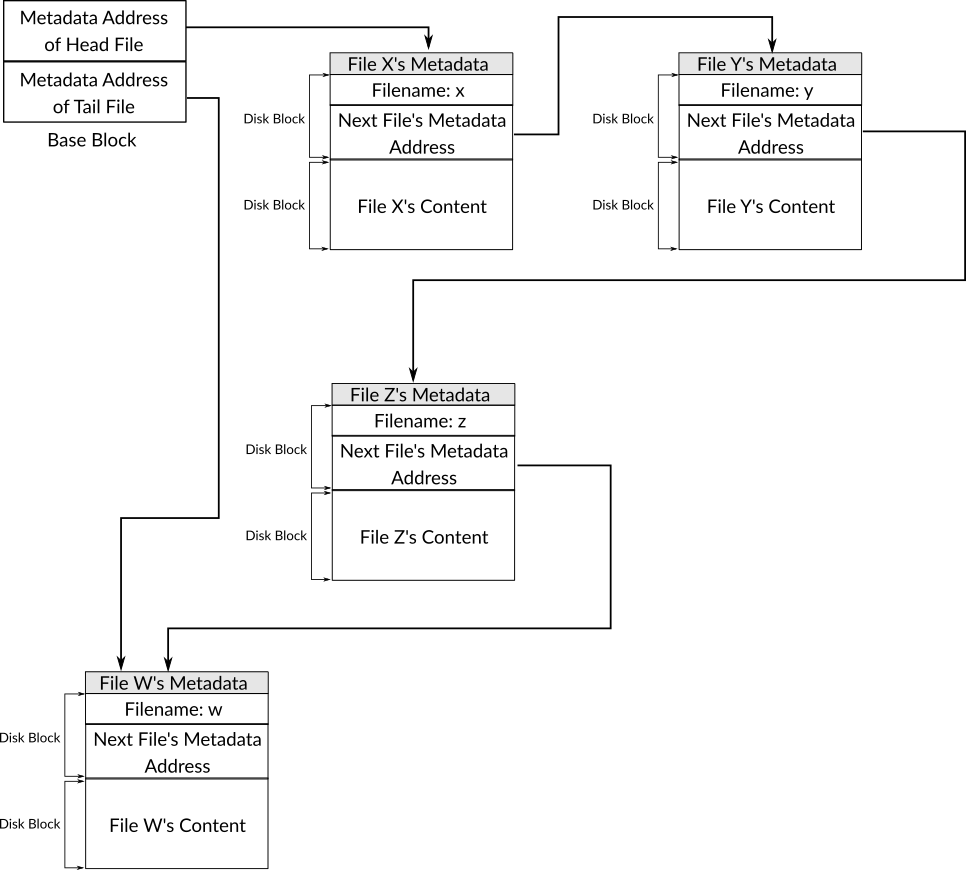
\includegraphics[width=0.75000\textwidth]{Figures/filesystem-ch/539filesystem_overview.png}
\caption{An Overview of 539filesystem
Design}\label{fig:539filesystem_overview}
\end{figure}

In 539filesystem, the block that has the address \lstinline!100! in the
disk is known as the \emph{base block}, from this block we can reach the
whole run-time filesystem. The base block is divided into two parts, the
size of each one of them is \lstinline!4! bytes, the first part is the
address of the metadata of the first file that has been created in the
run-time filesystem, that is, the \emph{head file} \footnote{In
  linked-list data structure's term: the head} while the second part is
the address of the metadata of the last file that has been created in
the run-time filesystem, that is, the \emph{tail file} \footnote{In
  linked-list data structure's term: the tail}.

Each file has its own metadata that contains file's name and the
\emph{next field} which stores the metadata address of the next file
that has been created. The length of the filename is \lstinline!256!
bytes and the size of ``next'' field is \lstinline!4! bytes. When there
is no next file, the value \lstinline!0! is stored in the ``next'' field
of the last file's metadata, that is, the tail file.

It should be obvious now how can we reach all files in a run-time
filesystem that uses 539filesystem, starting from the base block we get
the metadata address of the head file and by using the ``next'' field
from this metadata we can reach the metadata of the next file and the
process continues until we reach the tail file.

The metadata of each file is stored in the block right before the
content of the file which will be stored in one block only given that
the size of a block is \lstinline!512! bytes \footnote{In real-world
  situation, giving a whole block for a metadata of \lstinline!260!
  bytes can be considered as a waste of space. One of real filesystems
  goals is to use as little space as possible to maintain the structure
  of the run-time filesystem.}. For example, if the metadata of file
\lstinline!A! is stored in the address \lstinline!103!, then the content
of this file is stored in the address \lstinline!104!. By using this
design, the basic functionalities of filesystems can be provided. Figure
\ref{fig:539filesystem_overview} shows an overview of 539filesystem
design where four files stored in the system, \lstinline!x!,
\lstinline!y!, \lstinline!z! and \lstinline!w!.

\subsection{The Implementation of
539filesystem}\label{the-implementation-of-539filesystem}

Before getting started in implementing the proposed design in the
previous section, let's define two new files: \lstinline!str.h! and
\lstinline!str.c! which contain string related function that can be
useful when we write our filesystem. Two functions will be implemented
in \lstinline!str.c! and they are \lstinline!strcpy! which copies a
string from a location to another, and \lstinline!strcmp! which compares
two strings, if they are equals then \lstinline!1! is returned,
otherwise \lstinline!0! is returned. There is no need to explain the
details of the code of these two functions since they depend on the
normal way which C uses with strings. The following is the content of
\lstinline!str.h!.

\begin{lstlisting}[language=C]
void strcpy( char *, char * );
int strcmp( char *, char * );
\end{lstlisting}

The following is the content of \lstinline!str.c!.

\begin{lstlisting}[language=C]
#include "str.h"

void strcpy( char *dest, char *src )
{
    int idx = 0;
    
    while ( *src != '\0' )
    {
        dest[ idx ] = *src;
        
        src++;
        idx++;
    }
}

int strcmp( char *str1, char *str2 )
{
    while ( *str1 != '\0' )
    {
        if ( *str1 != *str2 )
            return 0;
        
        str1++;
        str2++;
    }
    
    if ( *str2 != '\0' )
        return 0;
    
    return 1;
}
\end{lstlisting}

Now we can start implementing 539filesystem. The first step as usual is
to create the files that hold the functions related to our filesystem:
\lstinline!filesystem.h! and \lstinline!filesystem.c!. The following is
the content of \lstinline!filesystem.h!.

\begin{lstlisting}[language=C]
#define BASE_BLOCK_ADDRESS 100
#define FILENAME_LENGTH 256

typedef struct
{
    int head, tail;
} base_block_t;

typedef struct
{
    char filename[ FILENAME_LENGTH ];
    int next_file_address;
} metadata_t;

base_block_t *base_block;

void filesystem_init();
void create_file( char *, char * );
char **list_files();
char *read_file( char * );

// Auxiliary Functions
metadata_t *load_metadata( int );
int get_address_by_filename( char * );
int get_prev_file_address( int );
int get_files_number();
\end{lstlisting}

First we define two macros, \lstinline!BASE_BLOCK_ADDRESS! and
\lstinline!FILENAME_LENGTH!. The first one is the address of base block
in the disk, as we have mentioned earlier, this address is
\lstinline!100!. The second one is the maximum length of a filename in
539filesystem, and we mentioned earlier that this length is
\lstinline!256!.

Then we define two structures as types: \lstinline!base_block_t! and
\lstinline!metadata_t!, based on our discussions on 539filesystem
design, you may have noticed that \lstinline!base_block_t! represents
the base block, it has two fields, each one of them of size
\lstinline!4! bytes, the first one is \lstinline!head! and the second
one is \lstinline!tail!. The type \lstinline!metadata_t! represents the
metadata of a file, it has two fields as we described before, the first
one is the filename and the second one is the metadata address of the
next file. These two structures are based on linked-list data structure,
and we are going to use them to load the data that they represent from
the disk, manipulate them while they are in the main memory, then write
them back to the disk in order to make the run-time filesystem
persistent.

Then the global variable \lstinline!base_block! is defined, which is the
memory address that contains the base block after loading it from the
disk, as we have said, this loaded copy is the one that we are going to
update when the user performs a transactional operation on the run-time
filesystem such as creating a new file for example.

After including \lstinline!filesystem.h! in \lstinline!filesystem.c! the
first function that we are going to implement is
\lstinline!filesystem_init! which is an initializer that will be called
once the kernel starts. Its code is too simple, it is going to use the
ATA device driver to read the base block from the disk to the main
memory and stores the memory address of this loaded data in the global
variable \lstinline!base_block!.

\begin{lstlisting}[language=C]
void filesystem_init()
{
    base_block = read_disk( BASE_BLOCK_ADDRESS );
}
\end{lstlisting}

We need to include \lstinline!filesystem.h! in \lstinline!main.c! and
call function \lstinline!filesystem_init! by putting the line
\lstinline!filesystem_init();! in \lstinline!kernel_main! of
\lstinline!main.c! after the line \lstinline!scheduler_init();!. The
rest of functions will be discussed in the following sub-sections.

\subsubsection{Creating a New File}\label{creating-a-new-file}

Let's begin with the function \lstinline!create_file!, we mentioned
before that there is no write operation in 539filesystem, instead, the
content of a new file is written in the same operation that creates a
new file. Basically, \lstinline!create_file! operation should decide the
disk address that the new file and its metadata should be stored in, of
course, in real-world situation, the filesystem should be sure that this
disk address is free and doesn't contain a part of another file. After
deciding the disk address of this new file, the metadata of the file
should be stored in the block that this address points to, and in the
next block the content of this file should be stored. The metadata of
the new file can be initialized by using the type \lstinline!metadata_t!
and after that it can be stored into the disk by using ATA device
driver.

Beside writing the metadata and the content of the file on the disk,
creating a new file in 539filesystem is equivalent to inserting a new
item in a linked-list, so, the base block need to be modified to make
sure that the new file is reachable later. To do that, the metadata
address of the new file should replace the tail in the base block, that
is, the metadata address that was the tail before creating the new file
is not the tail anymore, it become a normal item in the list that was
once the tail and it can be reached via the ``next'' field of the file
before it. The ``next'' field of this previous tail should be updated to
point to the newly created file, and the tail in base block should be
updated in the base block to point to the newly created file. There are
also more subtle cases in updating the base block that will be discussed
while writing the code of \lstinline!create_file!. Let's start with the
first part of the function.

\begin{lstlisting}[language=C]
void create_file( char *filename, char *buffer )
{
    int metadata_lba = ( base_block->head == 0 ) ? BASE_BLOCK_ADDRESS + 1 : base_block->tail + 2;
    int file_lba = metadata_lba + 1;
    
    metadata_t *metadata = kalloc( sizeof( metadata_t ) );
    
    metadata->next_file_address = 0;
    
    int currIdx;
    
    for ( currIdx = 0; *filename != '\0' && currIdx < FILENAME_LENGTH - 1; currIdx++, filename++ )
        metadata->filename[ currIdx ] = *filename;
    
    metadata->filename[ currIdx ] = '\0';
    
    write_disk( metadata_lba, metadata );
    write_disk( file_lba, buffer );
\end{lstlisting}

When the value of the head in the base block is \lstinline!0!, that
means there is no files at all in the run-time filesystem. When
\lstinline!create_file! is called in this situation, that means this
file that the caller is requesting to create is the first file in the
run-time filesystem, the metadata of this first file can be simply
stored in the block right after the base block. In
\lstinline!create_file! this fact is used to decide the disk address for
the metadata of the new file, this address is stored in the local
variable \lstinline!metadata_lba! which its name is a short for
``metadata logical block address''. Figure
\ref{fig:create_file_empty_case} shows the state of 539filesystem after
creating the first file \lstinline!A! in the run-time filesystem.

\begin{figure}
\centering
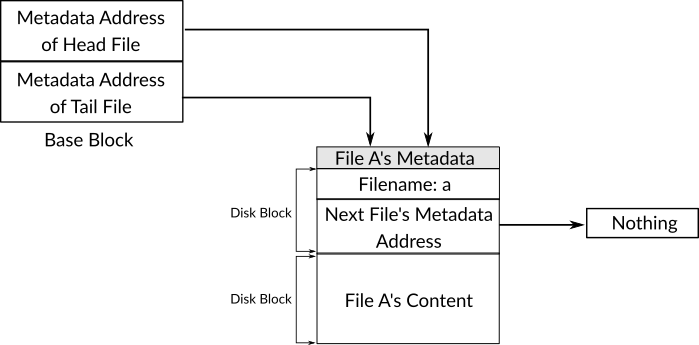
\includegraphics[width=0.65000\textwidth]{Figures/filesystem-ch/create_file_empty_case.png}
\caption{The State 539filesystem After Creating the First
File}\label{fig:create_file_empty_case}
\end{figure}

In case that the run-time filesystem is not empty, that is, the value of
\lstinline!head! is not \lstinline!0!, then the tail field of base block
can be used to decide the metadata address of the new file. As we know,
the tail field contains the metadata address of the last file that has
been added to the run-time filesystem, and the content of that file is
stored in the disk address \lstinline!tail + 1!, which means
\lstinline!tail + 2! is a free block that can be used to store new data
\footnote{This is ensured since 539filesystem stores the files in order,
  so, there will be no files after the tail unless it is a deleted file
  which can be overwritten and causes no data lose.}, so we choose this
address for the new metadata in this case. After that, the disk address
of the new content is decided by simply adding \lstinline!1! to the disk
address of the new metadata, the address of the content is stored in the
local variable \lstinline!file_lba!.

After deciding the disk addresses of the new metadata and file content,
we start in creating the metadata of the file to store them later on the
disk. As you can see in the code, we allocate a space in the kernel's
heap for the new metadata by depending on the type
\lstinline!metadata_t!, after this allocation, we can use the local
variable \lstinline!metadata! to fill the fields of the new file
metadata. First, we set the value of the ``next'' field to
\lstinline!0!, because, as we mentioned earlier, this new file will be
the tail file which means there is no file after it. Then, we copy the
filename which is passed as a parameter \lstinline!filename! to the
filename field of the metadata, in case the passed filename's length is
less than the maximum length, then the whole filename is copied,
otherwise, only the maximum number of characters of the passed filename
is copied and the rest are simply ignored. The final step that is
related to the new file is to write the metadata and the file content in
the right addresses on the disk, and this is done in the last two lines
which use the ATA device driver. The following is the next and last part
of \lstinline!create_file! which updates the base block depending on the
current state of the run-time filesystem.

\begin{lstlisting}[language=C]
    if ( base_block->head == 0 )
    {
        update_base_block( metadata_lba, metadata_lba );
    }
    else
    {   
        metadata_t *tail_metadata = load_metadata( base_block->tail );
        
        tail_metadata->next_file_address = metadata_lba;
        
        write_disk( base_block->tail, tail_metadata );      
        update_base_block( base_block->head, metadata_lba );
    }
} // End of "create_file"
\end{lstlisting}

When the run-time filesystem is empty, that is, the value of
\lstinline!head! in the base block is \lstinline!0!, then the new file
that we are creating will be both the head and the tail file. As you can
see, in the block of \lstinline!if! statement that checks whether
\lstinline!head! equals \lstinline!0! or not, the not defined yet
function \lstinline!update_base_block! is used, this function updates
the values of \lstinline!head! and \lstinline!tail! of the base block
and write these changes on the permanent copy of the base block on the
disk, the disk address of the new file's metadata is simply set as head
and tail when \lstinline!update_base_block! is called in this case.

The second case is when the run-time filesystem isn't empty, that is,
the value of \lstinline!head! isn't \lstinline!0!. In this case we need
to update the disk address of the tail in the base block to consider the
new file as the new tail, furthermore, the ``next'' field of the
previous tail, which is not the tail anymore, should be updated to point
to the metadata of the new file, you see in \lstinline!else! block that
this is exactly what is done.

The function that isn't defined yet \lstinline!load_metadata! is used to
load the metadata of the previous tail by passing the its disk address a
parameter. After that, the local variable \lstinline!tail_metadata! will
point to that loaded metadata of the tail, and depending on the type
\lstinline!metadata_t! we can reach the values of the previous tail
fields easily. You can see that we simply changed the value of the
``next'' field to the metadata address of the new file, then we write
this modification on the disk and of course on the same location,
finally, the tail field is updated in the base block by calling
\lstinline!update_base_block! which its code is presented next. Figure
\ref{fig:create_file_not_empty_case} shows the steps needed to create a
new file in 539filesystem as described and implemented in the function
\lstinline!create_file!.

\begin{lstlisting}[language=C]
void update_base_block( int new_head, int new_tail )
{
    base_block->head = new_head;
    base_block->tail = new_tail;
    
    write_disk( BASE_BLOCK_ADDRESS, base_block );
}
\end{lstlisting}

It's too simple, it receives the value of head and tail that we would
like to set on the base block, then, the copy of the base block which is
stored in the main memory is updated, then, this updated version is
overwritten on the base block address on the disk. The following is code
of \lstinline!load_metadata! which has been used in
\lstinline!create_file! function.

\begin{figure}
\centering
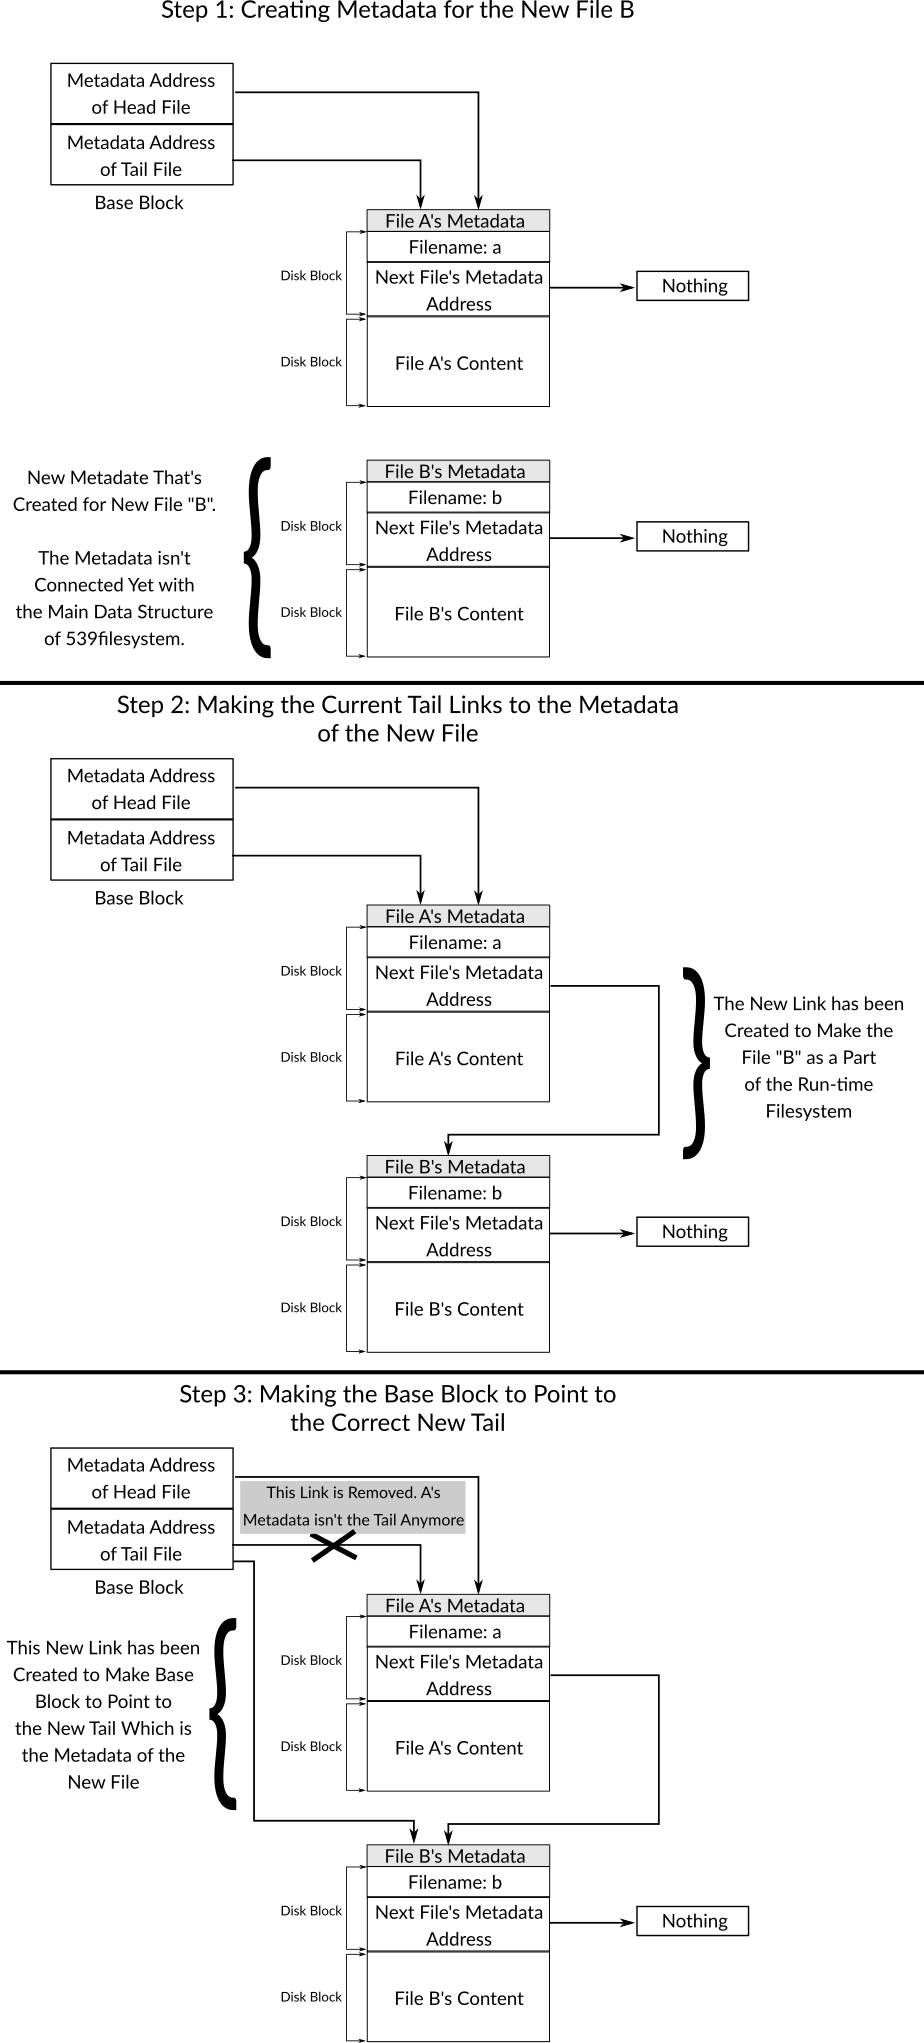
\includegraphics[width=0.85000\textwidth]{Figures/filesystem-ch/create_file_not_empty_case.png}
\caption{Steps Needed to Create New File in 539filesystem When Run-time
Filesystem isn't Empty}\label{fig:create_file_not_empty_case}
\end{figure}

\begin{lstlisting}[language=C]
metadata_t *load_metadata( int address )
{
    metadata_t *metadata = read_disk( address );
    
    return metadata;
}
\end{lstlisting}

Simply, it receives a disk address and assumes that the block which is
presented by this address is a metadata block. It loads this metadata to
the main memory by loading the content of the address from the disk
through the device driver function \lstinline!read_disk!. The following
is a sample of using \lstinline!create_file! to create a new file in the
run-time filesystem.

\begin{lstlisting}[language=C]
char *data = kalloc( 512 );

strcpy( data, "The content of the first file on 539filesystem" );
    
create_file( "first_file", data );
\end{lstlisting}

\subsubsection{Listing All Files}\label{listing-all-files}

To list all files on 539filesystem, the normal traversal algorithm of
linked-list can be used. In linked-list, to traverse all list's item you
need to start with the head of the list, then to reach the second item
of the list, the ``next'' field of the head can be used, and so on for
the rest of items in the linked-list. The ``next'' field is the
component which links the items of the list with each other. You keep
traversing the items until the tail of the list is reached and you can
check whether the current item is the tail or not by checking its
``next'' field, in case its value is \lstinline!0! (or usually in
higher-level implementations \lstinline!NULL!) then you know that the
current item is the tail which means the list is over. Another way to
check if the current item is the tail is by comparing its address with
the one which is stored in the tail field of the linked-list, in our
case, the base block. The following is the code of the function
\lstinline!list_files! which uses the algorithm we just described, it
returns an array of strings, each item of this array is a filename.

\begin{lstlisting}[language=C]
char **list_files()
{
    // Part 1
    
    if ( base_block->head == 0 )
        return -1;
    
    // Part 2
    
    char **list;
    
    list = kalloc( get_files_number() * sizeof( char * ) );
    
    // Part 3
    
    metadata_t *curr_file = load_metadata( base_block->head );
    
    int idx = 0;
    
    while ( 1 )
    {
        list[ idx ] = curr_file->filename;

        if ( curr_file->next_file_address == 0 )
            break;
        
        curr_file = load_metadata( curr_file->next_file_address );
        
        idx++;
    }
    
    return list;
}
\end{lstlisting}

The first part of \lstinline!list_files! handles the case where the
run-time filesystem is empty, so, it returns \lstinline!-1! to indicate
that there is no files to list. In case that the run-time filesystem
isn't empty, the function in the second part allocates a space in
kernel's heap for the list of the filenames, as you can see, we have
used a function named \lstinline!get_files_number! to decide how many
bytes we are going to allocate for this list, based on its name, this
function returns the number of files in the run-time filesystem, its
code will be presented in a moment. In the third part, the function is
ready to traverse the list of files metadata which are stored in the
disk and are reachable starting from the disk address which is stored in
the head field in the base block.

Initially, the metadata of the head file is loaded into memory and can
be accessed through the local variable \lstinline!curr_file!, then, the
loop is started. In the body of the loop, the filename of the current
file metadata is appended to the result's variable \lstinline!list!, in
the first iteration of this loop the filename will be the one that
belong to the head file. After appending the filename of the current
file to \lstinline!list!, the function checks if the current file is the
tail file or not by checking the value of the ``next'' field
\lstinline!next_file_address!, if it is \lstinline!0! then the current
file is the tail, so, the loop should break and the result should be
returned to the caller. In case that the current file isn't the tail
file, then the metadata of the next file is loaded by using the disk
address which is stored in the ``next'' field of the current file, the
current value of \lstinline!curr_file! is replaced with a memory address
that points to the metadata of the next file which will be used in the
next iteration of the loop, the same operation continues until the
function reaches the tail which breaks the loop and returns the list to
the caller. The following is the code of \lstinline!get_files_number!
that was used in \lstinline!list_files! and, as mentioned earlier,
returns the number of stored files.

\begin{lstlisting}[language=C]
int get_files_number()
{
    if ( base_block->head == 0 )
        return 0;
    
    int files_number = 0;
    
    // ... //
    
    metadata_t *curr_file = load_metadata( base_block->head );
    
    while ( 1 )
    {
        files_number++;

        if ( curr_file->next_file_address == 0 )
            break;
        
        curr_file = load_metadata( curr_file->next_file_address );
    }
    
    return files_number;
}
\end{lstlisting}

As you can see, it works in a similar way as \lstinline!list_files!, the
main difference is that \lstinline!get_files_number! keep tracking the
number of iterations to fetch the number of files instead of copying the
filename of the current file to another list. The following is a sample
of using \lstinline!list_files!.

\begin{lstlisting}[language=C]
void print_fs()
{
    char **files = list_files();

    for ( int currIdx = 0; currIdx < get_files_number(); currIdx++ )
    {
        print( "File: " );
        print( files[ currIdx ] );
        println();
    }
    
    print( "==" );
    println();
}
\end{lstlisting}

\subsubsection{Reading a File}\label{reading-a-file}

The function \lstinline!read_file! reads the content of a file which its
name is passed as a parameter, then, the address of the buffer that
stores that content of the file is returned to the caller. Because the
file size in 539filesystem is always \lstinline!512! bytes then
\lstinline!read_disk! of ATA device driver can be called just one time
to load a file.

To implement \lstinline!read_file!, the main thing to do is to find the
disk address of the file that the caller passed its name as a parameter,
after knowing how to traverse the list of files in 539filesystem, we can
easily use this algorithm to find the disk address of a file given its
name. The following is the code of \lstinline!read_file!.

\begin{lstlisting}[language=C]
char *read_file( char *filename )
{
    int address = get_address_by_filename( filename );
    
    if ( address == 0 )
        return 0;

    char *buffer = read_disk( address + 1 );
    
    return buffer;
}
\end{lstlisting}

The task of finding the disk address of the file's metadata is performed
by the function \lstinline!get_address_by_filename! which we will define
in a moment. When the metadata of the file is not found,
\lstinline!read_file! returns \lstinline!0!, otherwise, the file will be
read by calling \lstinline!read_disk!, as you can see, the parameter
that is passed to this function is \lstinline!address + 1! since the
value of \lstinline!address! is the disk address of the file's metadata
and not its content. Finally, the address of the buffer is returned to
the caller. The following is the code of
\lstinline!get_address_by_filename!.

\begin{lstlisting}[language=C]
int get_address_by_filename( char *filename )
{
    metadata_t *curr_file = load_metadata( base_block->head );
    int curr_file_address = base_block->head;
    
    int idx = 0;
    
    while ( 1 )
    {
        if ( strcmp( curr_file->filename, filename ) == 1 )
            return curr_file_address;
            
        if ( curr_file->next_file_address == 0 )
            break;
        
        curr_file_address = curr_file->next_file_address;
        curr_file = load_metadata( curr_file->next_file_address );      
    }
    
    return 0;
}
\end{lstlisting}

This function receives a filename as a parameter, then, it traverse the
list of the files, with each iteration, the name of the current file is
compared to the passed filename by using the function \lstinline!strcmp!
that we already defined, if the name of the current file doesn't match
the passed filename, the function loads the metadata of the next file by
using \lstinline!load_metadata! and continues to the next iteration of
the loop to check whether the next file is the required file or not, and
so on, if the file isn't found, then the loop exits and \lstinline!0! is
returned. When a match is found, the disk address of the current file's
metadata which is stored in the local variable
\lstinline!curr_file_address! is returned to the caller. The following
is a sample of using \lstinline!read_file!.

\begin{lstlisting}[language=C]
print( read_file( "first_file" ) );
\end{lstlisting}

\subsubsection{Deleting a File}\label{deleting-a-file}

As in creating a file, deleting a file may cause modifications on the
base block or even on another file's metadata. Given a filename, the
function \lstinline!delete_file! deletes this file from the run-time
filesystem, technically, the content of the file will not be overwritten
with zeros for example, instead, only the reference to this file is
removed from either the base block in case that file is the head, from
another file's ``next'' field or both in case that is file is the tail.

As mentioned earlier, this design decision of not overwriting the
content of the file, that the user would like to delete, with zeros for
example on the disk is taken in real-world filesystems to make the
delete process faster and this decision made it possible for deleted
files recovery software to exist, this type of software can recover
deleted files since their contents are still on the disk but there is
not reference to them in the run-time filesystem's data structure,
however, the space of deleted files are considered as free space by the
filesystem and it can be used anytime, that's why the recovery software
cannot ensure you that it could recover all deleted files because the
space which was occupied by the deleted file (or part of it) may be now
used by another file. The following is the code of
\lstinline!delete_file!.

\begin{lstlisting}[language=C]
void delete_file( char *filename )
{   
    // Part 1
    
    int curr_file_address = get_address_by_filename( filename );
    
    if ( curr_file_address == 0 )
        return;
    
    metadata_t *curr_file_metadata = read_disk( curr_file_address );
    
    // Part 2
    
    if ( get_files_number() == 1 )
    {
        update_base_block( 0, 0 );
        
        return;
    }
    
    // Part 3
    if ( curr_file_address == base_block->head )
    {
        update_base_block( curr_file_metadata->next_file_address, base_block->tail );
    }
    // Part 4
    else
    {
        int prev_file_address = get_prev_file_address( curr_file_address );
        
        metadata_t *prev_file = load_metadata( prev_file_address );

        prev_file->next_file_address = curr_file_metadata->next_file_address;
        
        write_disk( prev_file_address, prev_file );
        
        if ( curr_file_address == base_block->tail )
            update_base_block( base_block->head, prev_file_address );
    }
}
\end{lstlisting}

The first part tries to find the metadata address of the file in
question by using the function \lstinline!get_address_by_filename!, in
case the file is not found, the function does nothing and returns.
Otherwise, the metadata of the file is loaded and the local variable
\lstinline!curr_file_metadata! is used to point to that metadata in the
main memory.

In the second part, the most basic case of deleting a file is handled,
when there is only one file in the run-time filesystem, nothing need to
be done but updating the base block to indicate that the disk address of
both head and tail is \lstinline!0! which means, as mentioned earlier,
that the run-time filesystem is empty. The function
\lstinline!update_base_block! is used to update the base block. Figure
\ref{fig:delete_file_one_file_case} shows this case.

\begin{figure}
\centering
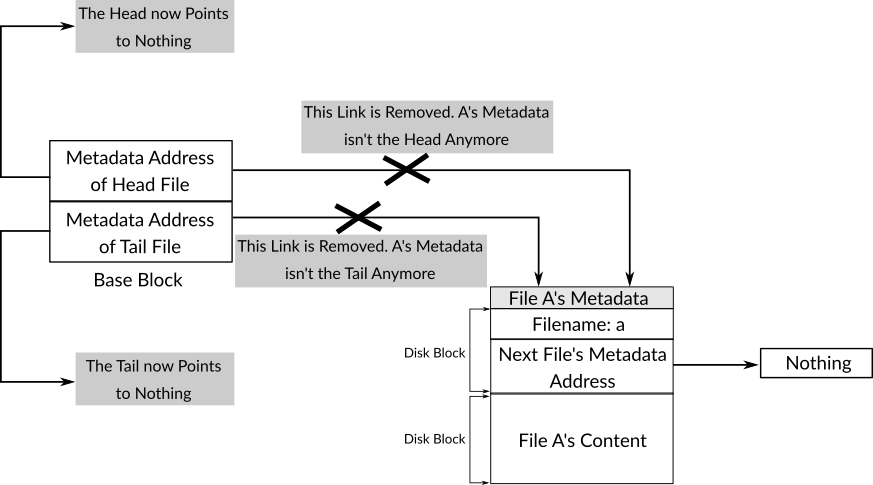
\includegraphics[width=0.80000\textwidth]{Figures/filesystem-ch/delete_file_one_file_case.png}
\caption{The State 539filesystem After Removing the Only
File}\label{fig:delete_file_one_file_case}
\end{figure}

The third part handles the case where the file to be deleted is the head
file, in this case, to remove the reference of this file, we simply
replace the current value of the \lstinline!head! in base block with the
metadata address of the file right next to the head which can be found
in the ``next'' field of the current head, so, the second file will
become the head file after finishing the delete process. Figure
\ref{fig:delete_file_head_case} shows this case.

\begin{figure}
\centering
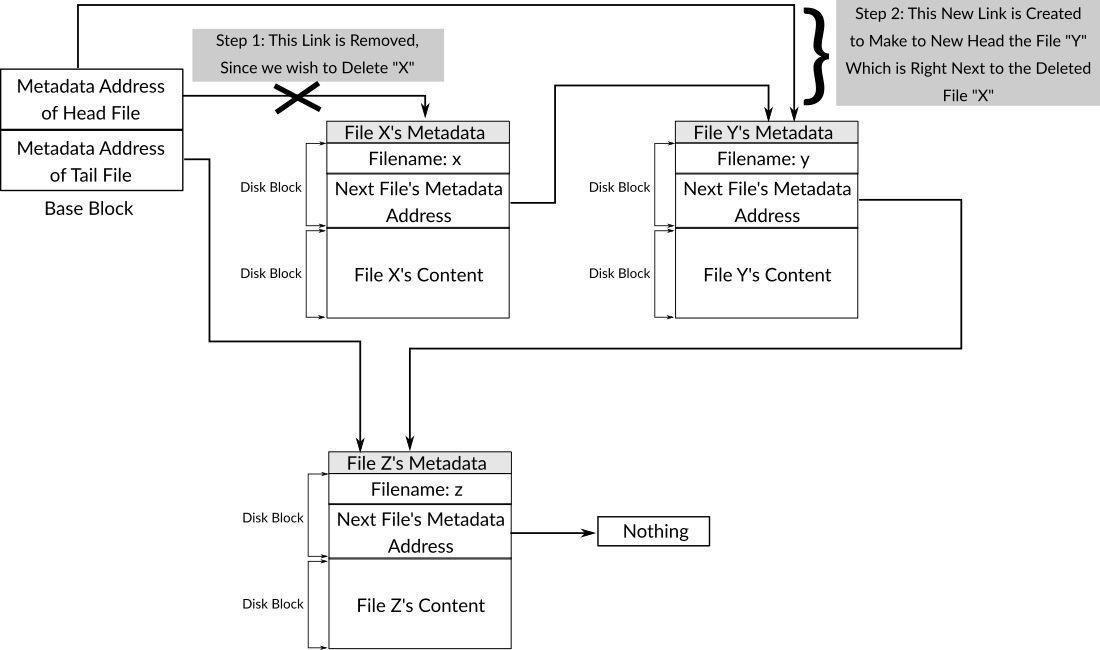
\includegraphics[width=1.00000\textwidth]{Figures/filesystem-ch/delete_file_head_case.png}
\caption{The Steps Needed to Delete the Head File in
539filesystem}\label{fig:delete_file_head_case}
\end{figure}

The fourth part of the function handles the case where the file to be
deleted is not the head, in this case, the previous file's metadata
needs to be found to modify its ``next'' field by replacing it with the
value of the ``next'' field of the file that we would like to delete, in
this way, we will be sure that the reference of the file to be deleted
is removed from 539filesystem data structure, and that the previous file
is linked with the next file. Figure \ref{fig:delete_file_not_head_case}
shows this case. Also, in this case, the file in question may be the
tail, therefore, the tail on the base block should be replaced with the
disk address of the previous file's metadata. Figure
\ref{fig:delete_file_not_head_but_tail_case} shows this case.

\begin{figure}
\centering
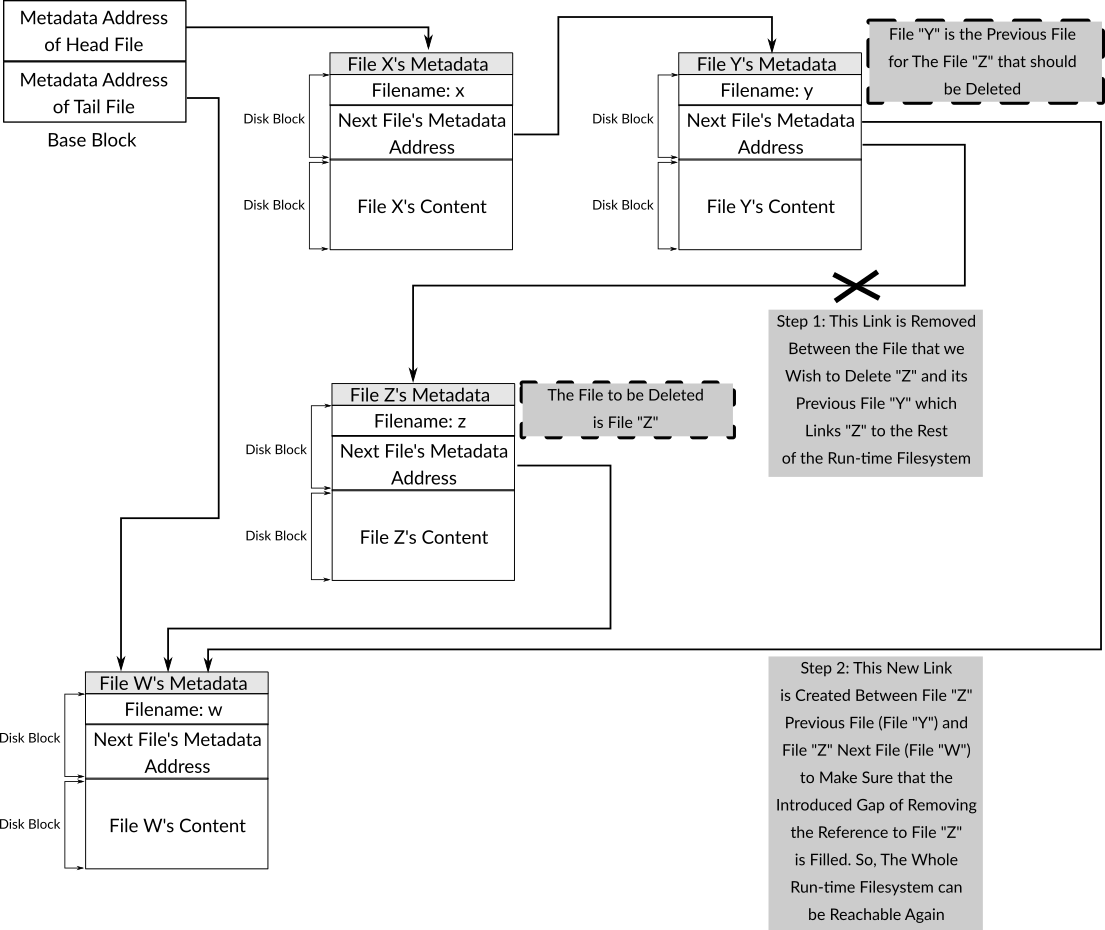
\includegraphics[width=1.00000\textwidth]{Figures/filesystem-ch/delete_file_not_head_case.png}
\caption{The Steps Needed to Delete a File which is not the
Head}\label{fig:delete_file_not_head_case}
\end{figure}

\begin{figure}
\centering
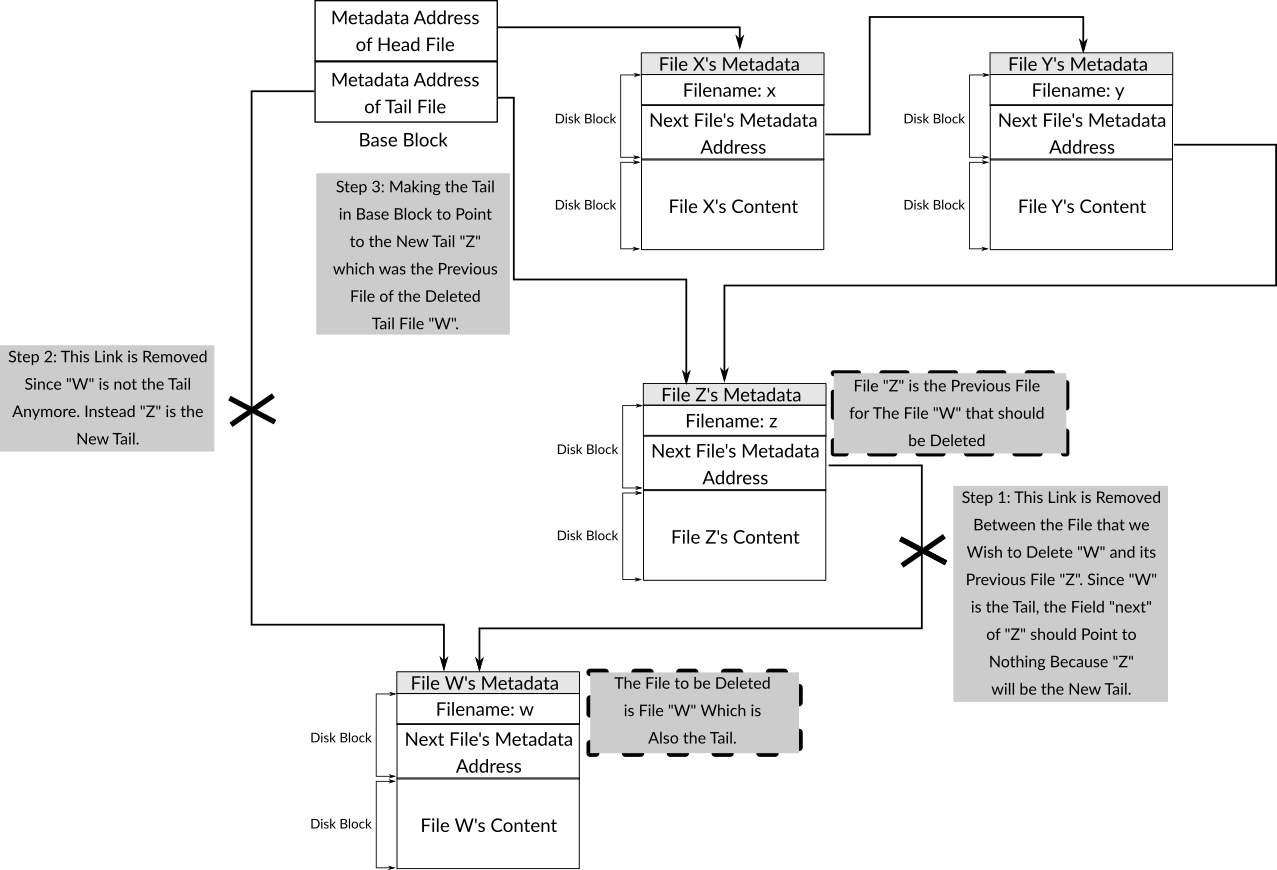
\includegraphics[width=1.00000\textwidth]{Figures/filesystem-ch/delete_file_not_head_but_tail_case.png}
\caption{The Steps Needed to Delete a File which is not the Head but
it's a Tail in 539filesystem. The File to Delete Here is
``W''.}\label{fig:delete_file_not_head_but_tail_case}
\end{figure}

As you can see in the first code line of this fourth part, a function
named \lstinline!get_prev_file_address! is used to get the disk address
of previous file's metadata to be able to perform the described
operation. By using this address, the metadata is loaded by using
\lstinline!load_metadata! in order to modify the ``next'' field of the
previous file, the updated metadata is written on the same address in
the disk. Finally, the function checks if the file to be deleted is the
tail file or not, if this is the case, the tail in base block is updated
to point to the previous file which ensures that there is no any
reference to that file in the filesystem's data structure. The following
is the code of \lstinline!get_prev_file_address! which needs no more
explanation.

\begin{lstlisting}[language=C]
int get_prev_file_address( int address )
{
    metadata_t *prev_file = load_metadata( base_block->head );
    int prev_file_address = base_block->head;

    while ( 1 )
    {
        if ( prev_file->next_file_address == address )
            return prev_file_address;
        
        prev_file_address = prev_file->next_file_address;
        prev_file = load_metadata( prev_file->next_file_address );
    }
        
    return -1;
}
\end{lstlisting}

\section{\texorpdfstring{Finishing up Version \texttt{NE} and Testing
the
Filesystem}{Finishing up Version NE and Testing the Filesystem}}\label{finishing-up-version-ne-and-testing-the-filesystem}

And now version \lstinline!NE! of 539kernel is ready. It contains a
basic ATA device driver and 539filesystem. The following is its
\lstinline!Makefile! which adds the new files to the compilation list,
also, this time we are going to use Bochs instead of QEMU to test
539filesystem since \lstinline!kernel.img! which represents the hardisk
is tailored for the former.

\begin{lstlisting}[language=make]
ASM = nasm
CC = gcc
BOOTSTRAP_FILE = bootstrap.asm 
SIMPLE_KERNEL = simple_kernel.asm
INIT_KERNEL_FILES = starter.asm
KERNEL_FILES = main.c
KERNEL_FLAGS = -Wall -m32 -c -ffreestanding -fno-asynchronous-unwind-tables -fno-pie
KERNEL_OBJECT = -o kernel.elf

build: $(BOOTSTRAP_FILE) $(KERNEL_FILE)
    $(ASM) -f bin $(BOOTSTRAP_FILE) -o bootstrap.o
    $(ASM) -f elf32 $(INIT_KERNEL_FILES) -o starter.o 
    $(CC) $(KERNEL_FLAGS) $(KERNEL_FILES) $(KERNEL_OBJECT)
    $(CC) $(KERNEL_FLAGS) screen.c -o screen.elf
    $(CC) $(KERNEL_FLAGS) process.c -o process.elf
    $(CC) $(KERNEL_FLAGS) scheduler.c -o scheduler.elf
    $(CC) $(KERNEL_FLAGS) heap.c -o heap.elf
    $(CC) $(KERNEL_FLAGS) paging.c -o paging.elf
    $(CC) $(KERNEL_FLAGS) ata.c -o ata.elf
    $(CC) $(KERNEL_FLAGS) str.c -o str.elf
    $(CC) $(KERNEL_FLAGS) filesystem.c -o filesystem.elf
    ld -melf_i386 -Tlinker.ld starter.o kernel.elf screen.elf process.elf scheduler.elf heap.elf paging.elf ata.elf str.elf filesystem.elf -o 539kernel.elf
    objcopy -O binary 539kernel.elf 539kernel.bin
    dd if=bootstrap.o of=kernel.img
    dd seek=1 conv=sync if=539kernel.bin of=kernel.img bs=512 count=20
    dd seek=21 conv=sync if=/dev/zero of=kernel.img bs=512 count=2046
    bochs -f bochs
\end{lstlisting}

To run Bochs, it should be configured properly. As you can see from the
presented \lstinline!Makefile!, a file named \lstinline!bochs! is passed
to Bochs to use it as a configuration file, so, by using it we don't
need to configure Bochs everytime we use it to run 539kernel. The
following is the content of \lstinline!bochs! file which should reside
in the same directory of 539kernel's code.

\begin{lstlisting}
plugin_ctrl: unmapped=1, biosdev=1, speaker=1, extfpuirq=1, parallel=1, serial=1, gameport=1, iodebug=1
config_interface: textconfig
display_library: x, options="gui_debug"
memory: host=32, guest=32
romimage: file="/usr/share/bochs/BIOS-bochs-latest"
vgaromimage: file="/usr/share/bochs/VGABIOS-lgpl-latest"
boot: disk
ata0: enabled=1, ioaddr1=0x1f0, ioaddr2=0x3f0, irq=14
ata0-master: type=disk, mode=flat, translation=auto, path="kernel.img", cylinders=2, heads=16, spt=63, biosdetect=auto, model="Generic 1234"
pci: enabled=1, chipset=i440fx
vga: extension=vbe, update_freq=5
cpu: count=1, ips=4000000, model=bx_generic, reset_on_triple_fault=1, cpuid_limit_winnt=0, ignore_bad_msrs=1, mwait_is_nop=0
cpuid: family=6, model=0x03, stepping=3, mmx=1, apic=xapic, sse=sse2, sse4a=0, sep=1, aes=0, xsave=0, xsaveopt=0, movbe=0, adx=0, smep=0, avx=0, avx_f16c=0, avx_fma=0, bmi=0, xop=0, tbm=0, fma4=0, vmx=1, x86_64=1, 1g_pages=0, pcid=0, fsgsbase=0, mwait=1
cpuid: vendor_string="GenuineIntel"
cpuid: brand_string="              Intel(R) Pentium(R) 4 CPU        "
\end{lstlisting}

As you can see, it tells Bochs the specifications of the virtual machine
we would like to run, also, the file which represents the hard disk
\lstinline!kernel.img! is passed to Bochs here. The following code can
be used to test 539filesystem. It should be inside
\lstinline!kernel_main! after the initializations and processes
creations.

\begin{lstlisting}[language=C]
    char *data = kalloc( 512 );
    strcpy( data, "The content of the first file on 539filesystem" );   
    create_file( "first_file", data );
    
    // ... //
    
    char *data2 = kalloc( 512 );
    strcpy( data2, "SECOND FILE in 539filesystem" );
    create_file( "second_file", data2 );
    
    // ... //
    
    char *data3 = kalloc( 512 );
    strcpy( data3, "THIRD FILE in 539filesystem" );
    create_file( "third_file", data3 );
        
    // ... //
    
    print( read_file( "first_file" ) ); println();
    print( read_file( "second_file" ) ); println();
    print( read_file( "third_file" ) ); println();
    
    // ... //
    
    print_fs();
    delete_file( "first_file" );
    print_fs();
\end{lstlisting}

This code creates three files, prints their contents, prints the
run-time filesystem tree through the function \lstinline!print_fs! and
finally deletes the file \lstinline!first_file! then prints the run-time
filesystem tree again to show that the file has been deleted
successfully. The function \lstinline!print_fs! already defined in this
chapter. To make everything works file, you need to keep the definition
of \lstinline!print_fs! below \lstinline!kernel_main! and put the
prototype \lstinline!void print_fs();! above \lstinline!kernel_main!.
Also, to test the filesystem you need to make sure that the interrupts
are disabled, the easiest way to do that is modifying
\lstinline!starter.asm! by commenting the line \lstinline!sti! which is
before \lstinline!call kernel_main! in the routine
\lstinline!start_kernel!. After that you should see the result of the
above testing code after the kernel boots up.

    \chapter{Chapter 7: What's Next?}\label{ch-wthat-is-next}

\section{Introduction}\label{introduction}

And now, after writing a simple operating system's kernel and learning
the basics of creating kernels, the question is ``What's Next?''.
Obviously, there is a lot to do after creating 539kernel and the most
straightforward answers for our question are the basic well-known
answers, such as: implementing virtual memory, enabling user-space
environment, providing graphical user interface or porting the kernel to
another architecture (e.g.~ARM architecture). This list is a short list
of what you can do next with your kernel.

Previously, I've introduced the term \emph{kernelist} \footnote{In
  chapter \ref{ch-progenitor} where the distinction between a kernelist
  and a traditionalist has been established.} in which I mean the person
who works on designing operating system kernels with modern innovative
solutions to solve real-world problem. You can continue with your hobby
kernel and implement the well-known concepts of traditional operating
systems that we have just mentioned a little of them, but if you want to
create something that can be more useful and special than a traditional
kernel, then I think you should consider playing the role of a
kernelist.

If you take a quick look on current hobby or even production operating
system kernels through GitHub for example, you will find most of them
are traditional, that is, they focus on implementing the traditional
ideas that are well-known in operating systems world, some of those
kernels go further and try to emulate another previous operating system,
for example, many of them are Unix-like kernel, that is, they try to
emulate Unix. Another examples are ReactOS\footnote{\url{https://reactos.org/}}
which tries to emulate Microsoft Windows and Haiku\footnote{\url{https://www.haiku-os.org/}}
which tries to emulate BeOS which is a discontinued proprietary
operating system. Trying to emulate another operating systems is good
and has advantages of course, but what I'm trying to say that there are
a lot of projects that focus on this line of operating systems
development, that is, the traditionalists line and I think the line of
kernelists needs to be focused on in order to produce more innovate
operating systems.

I've already said that the kernelist doesn't need to propose her own
solutions for the problems that she would like to solve. Instead of
using the old well-known solutions, a kernelist searches for other
better solutions for the given problem and designs an operating system
kernel that uses these solutions. Scientific papers (papers for short)
are the best place to find novel and innovative ideas that solve
real-world problem, most probably, these ideas haven't been implemented
or adopted by others yet\footnote{Scientific papers can be searched for
  through a dedicated search engine, for example, Google Scholar.}.

In this chapter, I've chosen a bunch of scientific papers that propose
new solutions for real-world problem and I'll show you a high-level
overview of these solutions and my goal is to encourage interested
people to start looking to the scientific papers and implement their
solutions to be used in the real-world. Also, I would like to show how
the researches on operating systems field (or simply the kernelists!)
innovate clever solutions and get over the challenges, this could help
an interested person in learning how to overcome his own challenges and
propose innovate solutions for the problem that he faces.

Of course, the ideas on the papers that we are going to discuss (or even
the other operating system's papers) may need more than a simple kernel
such as 539kernel to be implemented. For example, some ideas may need a
networking stack being available in the kernel, which is not available
in 539kernel, so, there will be two options in this case, either you
implement the networking stack in your kernel or you can simply focus on
the problem and solution that the paper present and use an already exist
operating system kernel which has the required feature to develop the
solution upon this chosen kernel, of course, there are many open source
options and one of them is HelenOS\footnote{\url{http://www.helenos.org/}}
microkernel\footnote{The concept of \emph{microkernel} will be explained
  in this chapter.}.

A small note should be mentioned, this chapter only shows an overview of
each paper which means if you are really interesting on the problem and
the solution that a given paper represents, then it's better to read it.
It is easy to get a copy of any mentioned paper in this chapter, you
just need to search for its title in Google Scholar
(\url{https://scholar.google.com/}) and a link to a PDF will show for
you. However, before getting started in discussing the chosen papers, I
would like in the next subsection to discuss a topic that I've deferred
till this point, this topic is related to the architecture design of a
kernel.

\subsection{The Design of Kernel's Architecture: Monolithic
vs.~Microkernel}\label{the-design-of-kernels-architecture-monolithic-vs.microkernel}

The architecture of an operating system, as in any other software, can
be designed in many different ways and the most commonly known kernel's
architecture are \emph{monolithic} and \emph{microkernel}. When the
monolithic architecture is used in a kernel, the whole code of the
kernel runs in the kernel-mode, that is, all the code of the kernel
(hence, all its different modules) has the same privileges to perform
any operation and to change anything in the system, even the device
drivers. A notable example of monolithic kernels is Linux, also, the
modern BSD family (FreeBSD, NetBSD and OpenBSD) uses the monolithic
architecture, the original Unix itself used a monolithic kernel. As you
may notice, 539kernel is also a monolithic kernel.

The other well-known design is microkernel, where not every component of
an operating system kernel is run as a privileged code (in kernel-mode),
instead, only the code that really needs to perform privileged
instructions. The other parts of the kernel that doesn't need to perform
privileged instructions are separated from the microkernel and run in
the user-mode as any other user application and they are known as
\emph{servers} in microkernel architecture. The goal of those servers is
providing an interface that represents the kernel services for the user
applications, and when a privileged instructions needed to be performed,
the server communicates with the microkernel which runs in kernel-mode
to do so. For example, when a user process needs to create a new
process, it needs to communicate with \emph{processes server} which runs
in user-mode and request from it to create a new process. The processes
server maintains the processes list and their process control block
since these data structures don't need to be in the kernel-mode or
kernel's address space, so, when a process creation request arrives, the
creation of the new entry for the new process will be the responsibility
of the processes server with no need to run any privileged code, once a
privileged code is needed, the microkernel will be called by the server.

Let's take process management module of 539kernel as example. This
module provides one function which is \lstinline!process_create! in
\lstinline!process.c!, if you read the code of this module you will see
there is no any part of it needs to run in kernel-mode. That means, if
539kernel was a microkernel, this whole module can run as a userspace
server instead of being in the kernel itself. Another example from
539kernel is the scheduler, you can see for example in the function
\lstinline!scheduler! (\lstinline!scheduler.c!) that there is no need to
run it in the kernel-mode, so, if 539kernel was a microkernel, this
module can be run as a separated userspace server instead. If you review
the code of \lstinline!scheduler! carefully, you can see that it needs
to reach the processes list and also needs to modify the processes
control block, that's mean the scheduler server needs to communicate
with processes server to perform these operations. In microkernels this
can be done through message passing, for example, the scheduler server
can send a message to the processes server to get the ready processes
list or to change some attribute in a process control block and so on,
the same is applicable between the other servers. The function
\lstinline!run_next_process! in \lstinline!scheduler.c! is an example
from 539kernel's scheduler module that needs to run as privileged code,
so, if 539kernel was a microkernel this function should reside in the
kernel itself and not in the scheduler server. Another example of
539kernel that should be in the kernel itself instead of the server is
the interrupt handler \lstinline!isr_32! in \lstinline!idt.asm!.

The goal of microkernel design is keeping the code that needs to run as
privileged code as small as possible and move all the other code to the
userspace. This can make the kernel itself more secure, reliable and
easier to debug. Microkernels have a long history of research to improve
its performance and make it better, there are many microkernels
available nowadays, for example, L4, Mach which has been used in
NeXTSTEP operating system that the current macOS based on \footnote{Though,
  macOS' kernel is considered as a hybrid kernel and not a microkernel.},
Minix, HelenOS and Zircon which is the kernel of Fuchsia operating
system and maybe one of the famous microkernel's related stuff is a
debate known as \emph{Tanenbaum--Torvalds debate} between Andrew S.
Tanenbaum (the creator of Minix and the author of the book ``Operating
Systems: Design and Implementation'') and Linus Torvalds (the creator of
Linux) in 1992 after few months Linux kernel release\footnote{The title
  of the post which started the debate was ``LINUX is obsolete'' by
  Andrew Tanenbaum. The text of the debate is available online here:
  \url{https://www.oreilly.com/openbook/opensources/book/appa.html}}.

\section{In-Process Isolation}\label{in-process-isolation}

In current operating systems, any part of a process can read from and
write to any place of the same process' memory. Consider a web browser
which like any other application consists of a number of different
modules (in the perspective of programmers) and each one of them handles
different functionality, rendering engine is one example of web
browser's module which is responsible for parsing HTML and drawing the
components of the page in front of the user. When an application is
represented as a process, there will be no such distinction in the
kernel's perspective, all application's modules are considered as one
code that each part of it has the permission to do anything that any
other code of the same process can do.

For example, in web browser, the module that stores the list of web
pages that you are visiting right now is able to access the data that is
stored by the module which handles your credit card number when you
issue an online payment. As you can see, the first module is much less
critical than the second one and unfortunately if an attacker can
somehow hack the first module through an exploitable security bug, she
will be able to read the data of the second module, that is, your credit
card information and nothing is going to stop her.

This happens due to the lack of \emph{in-process isolation} in the
current operating systems, that is, both sensitive and insensitive data
of the same process are stored in the same address space and any part of
the process code is permitted to access all these data, so, there is no
difference in your web browser's process between the memory region which
stores that titles of the pages and the region which stores you credit
card information. A severe security bug known as \emph{HeartBleed
vulnerability} showed up due to the lack of in-process isolation. Next,
two of the solutions for the problem of data isolation that has been
proposed by kernelists will be discussed.

\subsection{Lord of x86 Rings}\label{lord-of-x86-rings}

A paper named ``Lord of the x86 Rings: A Portable User Mode Privilege
Separation Architecture on x86'' \footnote{Authored by Hojoon Lee,
  Chihyun Song and Brent Byunghoon Kang. Published on 2018.} proposes an
architecture (named LOTRx86 for short) which provides an in-process
isolation, the paper uses the term \emph{user-mode privilege separation}
which has the same meaning. LOTRx86 doesn't use the new features of the
modern processors to implement the in-process isolation, Intel's
Software Guard Extensions (SGX) is an example of these features. The
reason of not using such modern feature in LOTRx86 is portability, while
SGX is supported in Intel's processors, it is not in AMD's
processors\footnote{Beside Intel, also AMD provides processors that use
  x86 architecture.} which means that employing this feature will make
our kernel only works on Intel's processor and not AMD's. Beside that,
SGX is a relatively new technology\footnote{Intel's SGX is deprecated in
  Intel Core but still available on Intel Xeon.} which means even older
Intel's processors don't support it and that makes our kernel less
portable and can only run on specific types of Intel's processors. So,
if we would like to provide in-process isolation in our kernel, but at
the same time, we want it to work on both Intel's and AMD's processors,
that is, portable \footnote{In LOTRx86 when the term \emph{portable} is
  used to describe something it means that this thing is able to work on
  any modern x86 processor. The same term has another boarder meaning,
  for example, if we use the boarder meaning to say ``Linux kernel is
  \emph{portable}'' we mean that it works on multiple processors
  architecture such as x86, ARM and a lot more and not only on Intel's
  or AMD's x86.}, what should we do? According to LOTRx86, we use
privilege levels to do that.

Throughout this book, we have encountered x86 privilege levels and we
know from our previous discussions that modern operating systems only
use the most privileged level \lstinline!0! as kernel-mode and the least
privileged level \lstinline!3! as user-mode. In LOTRx86 a new area in
each process called \emph{PrivUser} is introduced, this area keeps the
sensitive data of the process and it's only accessible through special
code that runs on the privilege level \lstinline!2!, so, in a kernel
which employs LOTRx86 a process may run in privilege level \lstinline!3!
(user-mode), as in modern operating systems, and may run in privilege
level \lstinline!2! (PrivUser). Most of the normal work of a process
will be done in level \lstinline!3!, but when the code is related to
sensitive data, such as storing, accessing or processing them, the
process will run on level \lstinline!2!. Of course, the sensitive data
cannot be accessed by process' normal code since the latter runs on
level \lstinline!3! and the former needs a code that runs on privilege
level \lstinline!2! to be accessed. If an attacker exploit a
vulnerability that allows him to read the memory of the process, he will
not be able to read the secret data if this vulnerability is on the
normal code of the process.

A kernel with LOTRx86 should provide a way for the programmers to use
the feature provided by LOTRx86, so, the authors of the paper propose a
programming interface named \emph{privcall} which works like Linux
kernel's system calls. Through this interface an application programmer
can write functions (routines) that process the secret data, these
functions will run on privilege level \lstinline!2! and will be stored
in PrivUser, we will call these functions as \emph{secret functions} in
our coming discussion. When the normal code of the process need to do
something with some secret data that is stored in PrivUser a specific
secret function can be called through \lstinline!privcall! interface,
once this call is issued, the current privilege level will be changed
from \lstinline!3! (user-mode) to \lstinline!2! (PrivUser\footnote{In
  the paper, the name PrivUser means two things, the execution mode and
  the secret memory area.}) by using x86 call gates. Note that this
solution \textbf{mitigates} vulnerabilities like HeartBleed but doesn't
\textbf{prevent} them necessarily.

To implement this architecture, two requirements should be satisfied in
order to reach the goal. The first requirement is called
\lstinline!M-SR1! in the paper and it states that the PrivUser area
should be protected from the normal user mode which most of the
application's code run on. The second requirement is called
\lstinline!M-SR2! in the paper and it states that the kernel should be
protected from PrivUser code.

To satisfy the first requirement, the pages of PrivUser are marked as
privileged pages in their page entry \footnote{We have discussed this
  bit in a page entry in chapter \ref{ch-process-management}.}, that is,
the code that run on privilege level \lstinline!3! cannot access them
while the code that runs on levels \lstinline!0!, \lstinline!1! and
\lstinline!2! can. To satisfy the second requirement, the authors
propose to use segmentation, \lstinline!LDT! table is employed to
divided each process into segments and a special segment for the secret
functions and data, that is, PrivUser is defined and the definition of
this segment indicates that the secret functions can only access the
secret data under privilege level \lstinline!2! in order to protect the
kernel's data which reside in privilege level \lstinline!0!.

This was the high-level description of LOTRx86 solution, there are some
challenges that have been faced by the authors and the details of them
and how they overcame them can be found in the paper, so, if you are
interested on implementing LOTRx86 in your kernel, I encourage you to
read the original paper which also discusses how the authors managed to
implement their solution in Linux kernel as kernel modules, also, the
paper shows the performance evaluation of their implementation. There is
something to note, the authors assume that the solution is implemented
in \lstinline!64-bit! environment instead of \lstinline!32-bit! and due
to that they faced some challenges that the may not be faced in
\lstinline!32-bit! environment.

Of course LOTRx86 is not the only proposed solution for our problem,
there are a bunch more and some of them are mentioned on the same paper
that we are discussing. What makes LOTRx86 differs from them is the
focus on a solution that has a better performance and portable as we
have examined in the beginning of this subsection.

As you saw in this solution how the authors played the role of a
kernelist, they proposed a solution for real-world problem, they used
some hardware feature that is usually used in a different way in the
traditional operating systems (privilege level \lstinline!2!) and they
proposed a different and useful idea for operating system kernels.

\subsection{Endokernel}\label{endokernel}

The proposed solution In LOTRx86 paper isolates the memory within the
process but what about the other system resources (e.g.~files)? For
example, what if a critical module in the process needs to read and
write on a secret file while the other modules of the same process
should not reach this file at all. The only system resource that LOTRx86
protects is the memory while the other resources of the system are
accessible by any module within the process.

The paper ``The Endokernel: Fast, Secure, and Programmable Subprocess
Virtualization'' \footnote{Authored by: Bumjin Im, Fangfei Yang,
  Chia-Che Tsai, Michael LeMay, Anjo Vahldiek-Oberwagner and Nathan
  Dautenhahn. Published on 2021.} proposes a solution to handle this
case by modifying the traditional process model which used by most
modern operating systems. In Endokernel Architecture a monitor is
attached within each process. This monitor, which is called endokernel,
isolates itself from the untrusted parts of the process and also
provides a lightweight virtual machine, called endoprocess, to the rest
of the process and through defined polices the isolation can be
enforced, for example, some processor's instructions can be permitted to
be executed by the untrusted parts of the process without monitoring but
some other can be defined that the should be monitored. Also, the
filesystem's operations that are allowed to be used can be defined by
the policies and the endokernel is going to ensure that these policies
are enforced.

\section{Nested Kernel}\label{nested-kernel}

In monolithic design, the kernel is considered as one entity and each
component of the kernel is able to read/modify the data and maybe the
code of another component since the whole of the kernel's code works on
kernel mode. Beside the standard components of the kernel (e.g.~process
management and memory management), usually, the device drivers are
considered as a part of the monolithic kernel and they run on the kernel
mode, these device drivers are, most probably, written by a third party
entity which makes them considered as an untrusted code, also, they may
be buggy if they are compared to the standard code of the kernel. Any
exploitable bug in any part of a monolithic kernel (either in a device
driver or not) will give the attacker the access to the whole kernel.
This problem reminds us with the problem which has been presented
earlier in this chapter but this time the kernel is the one which
suffers from it.

Microkernel design solves this problem by separating the most components
of the kernel as user-space servers, but what if we would like to keep
the monolithic design and have this kind of separation? This is what a
paper titled ``Nested Kernel: An Operating System Architecture for
Intra-Kernel Privilege Separation'' \footnote{Authored by Nathan
  Dautenhahn, Theodoros Kasampalis, Will Dietz, John Criswell and Vikram
  Adve. Published on 2015.} is trying to do by proposing a new kernel's
design called \emph{nested kernel}.

Memory is the root of all evil, that's what I feel this paper is trying
to tell us. In nested kernel design, the operating system kernel is
divided into two parts, the first one is nested kernel and the second
part is \emph{outer kernel}. The nested kernel is isolated from the
outer kernel and both parts run on kernel mode. The job of nested kernel
is to isolate the memory management unit (MMU) from the outer kernel. To
make the outer kernel able to use the functionality that MMU provides,
the nested kernel exposes and controls an interface of the MMU, this
interface is called \emph{virtual MMU} (\emph{vMMU}) in the paper, so,
if any part of the outer kernel needs to manipulate the state of MMU
then vMMU interface can be used. The nested kernel part has small and
trusted code while the outer kernel contains all other code that cannot
be trusted (e.g.~device drivers) or may be buggy. When we say isolating
MMU we mean that the data structures and registers that build the state
of MMU are isolated, so, in x86 for example, isolating MMU means
isolating page directory, page tables and the control registers that are
related to paging.

The memory regions which a kernel implementer would like to protect from
being modified by the outer kernel (protected memory) are marked as
read-only region in nested kernel design and only the nested kernel has
the permission to modify them. For example, say that you have decided to
protect the memory that contains the code of the kernel which checks if
the current user has the permissions to read or modify a specific file,
this region can by marked as read-only and can be protected by the
nested kernel all the time from being modified by any part of the outer
kernel. Now, assume that an attacker found an exploitable security bug
in one of the device drivers, and his goal is to modify that code of
permission checking in order to let him to read some critical file, this
cannot be done since the memory region is protected and read-only, the
paper discusses how in details how to ensure that the outer kernel
doesn't violate the protection of nested kernel in x86 architecture.

That's not the whole story. Making the nested kernel the only way to
modify the protected memory by the outer kernel means that the nested
kernel can be a mediator which will be called before any modification
performed. This will let the kernel's implementer to define security
policies and enforce them while the system is running. For example, the
authors propose \emph{no write policy} which doesn't let the outer
kernel to write on a specific memory region at all (e.g.~the example of
checking permissions code). Another proposed policy is \emph{write-once
policy} which lets the outer kernel to write to a region of memory just
one time, this policy will be useful with the memory region that
contains the \lstinline!IDT! table for example, so, the attacker cannot
modify the interrupt service routines after setting them up by the
trusted code of outer kernel. More policies were presented in the paper.
You can see here how the kernelists proposed a new kernel design other
than the popular ones (microkernel and monolithic) in order to solve a
specific real-world problem.

\section{Multikernel}\label{multikernel}

The paper ``The Multikernel: A new OS architecture for scalable
multicore systems'' \footnote{Authored By: Andrew Baumann, Paul Barham,
  Pierre-Evariste Dagand, Tim Harris, Rebecca Isaacs, Simon Peter,
  Timothy Roscoe, Adrian Schüpbach and Akhilesh Singhania. Published in
  2009.} shows a good example of kernelists who get rid of the old
designs completely in order to provide a modern one which is more
suitable for current days. In the paper, the authors have observed the
new trends in the modern hardware, these trends motivated them to
propose a new kernel architecture named \emph{multikernel}. One of these
observations is the diversity of the new systems, according to the
authors, the operating systems in the new systems need to work with
machines that may have cores with different instruction set
architectures, that is, they have heterogeneous cores, either in term of
instruction set architecture or performance. Another observation is that
the message passing is now easier in the modern hardware and can be used
instead of shared memory in order to share information between two
processes for example, the idea of multikernel aims to handle these
observations and provide an architecture of a kernel that is suitable
for the modern multicore systems.

In multikernel architecture, a multicore system is handled as a network
of cores, as if each core is a separate processor, and the
communications between the cores are performed through message passing,
it is not necessary that the cores belong to the same machine. When the
cores are handled as a network of machines, the algorithms and
techniques of distributed systems can be used.

The design of multikernel depends on three principles. First, all
communications between the cores in the kernel should be explicit
through message passing and no implicit communications (e.g.~through
shared memory) is allowed, one of the benefits of this principle is the
ability to use well-known networking optimizations in order to make the
communications between cores more efficient. Also, making the
communication explicit can help in reasoning about the correctness of
the kernel's code. The second principle is separating the structure of
the operating system as much as possible from the hardware, that is, the
structure should be hardware neutral. The benefits of this principle are
obvious and one of them is making the adaptation of processor's specific
optimization easier \footnote{The paper mentioned that applying one of
  optimizations on Windows 7 caused changes in \lstinline!6,000! lines
  of code through \lstinline!58! files.}. The last principle is dealing
with the state of the operating system (e.g.~processes table) as
replicated instead of shared, that is, when a core need to deal with a
global data structure, a copy of this data structure is sent to this
core instead of using just one copy by all the cores in the system.
Based on these design principles, the authors built an implementation
called Barrelfish, according to the authors, this implementation is an
example of multikernel but not the only way to build one. The paper
discusses in details how they designed Barrelfish to realize
multikernel's design principles and how they overcame the challenges
that the have faced.

\section{Dynamic Reconfiguration}\label{dynamic-reconfiguration}

Changing a specific module while the system is running can be an
important aspect in some systems, for most desktop users, when some
module of a system is changed, due to updating the system for example,
it will be fine to reboot the system to get the new changes applied, but
what about a server that needs to run all the time with no downtime,
rebooting it is not an option. Current operating systems still require a
reboot when an update to specific parts is performed, for example,
updating Linux kernel in a running system requires a reboot to this
system to be able to use the new version of the kernel.

Dynamic reconfiguration is the process of changing a specific module of
the system while keeping it running without the need of rebooting it,
that's how a paper titled ``Building reconfigurable component-based OS
with THINK'' \footnote{Authored by: Juraj Polakovic, Ali Erdem Özcan and
  Jean-Bernard Stefani. Published on 2006} defines this term. According
to the paper, dynamic reconfiguration consists of the followings steps:
First, the part that we would like to reconfigure (the reconfiguration
target) should be identified and separated from other parts, to do that,
THINK framework uses a component model called Fractal \footnote{\url{https://fractal.ow2.io/}}
in order to identify each part of the system as a separated component,
after that, the process of reconfiguration is going to deal with these
components, for example, in 539kernel the process management part, the
scheduler, the memory management part, the allocator and the filesystem
can be defined as separated components, as you can see each of these
part has its own functionality and can be encapsulated, by using dynamic
reconfiguration we can for example change the current scheduler with
another one while the system is running.

The second step is to make sure that the reconfiguration target is on
the safe state, that is, there is no other part that is using the target
right now, thread counting is one technique that has been proposed in
the paper to detect safe state, when employing this technique any call
to a component causes the thread counter to increase by \lstinline!1!
and when this call finishes the thread counter decreases by
\lstinline!1!, a component is on the safe state when the thread counter
is \lstinline!0!, that is, no thread (or process) is currently using the
target component. After the target component reaches the safe state it
can be changed to the new component, the context of the target should be
moved to the new component and after that the execution of the component
can be resumed.

\section{Unikernel}\label{unikernel}

Virtualization is widely used today and cloud computing is an obvious
example of employing virtualization technologies. Nowadays, you can
easily start and stop virtual machines that run a commodity operating
system (e.g.~Linux or Windows) and via this virtual machine you can run
whatever software you wish as if this virtual machine is a real one.
There are many cases where a virtual machine is used to provide just one
thing, for example, a virtual machine that runs a web server solely. To
do that, of course an operating system is needed to be installed in the
virtual machine, say for example Linux, and of course a web server
should be installed on top this operating system, say Apache. Linux (and
modern general purpose operating systems) is a multiprocess and
multiuser kernel which contains a lot of code that handle the protection
of the processes, the users and the kernel itself (via the separation of
kernel-mode and user-mode as we have discussed through this book),
beside that, there are a lot of services that are provided in general
purpose operating systems so they can be suitable for all users.

In our example of the virtual machine which only runs a web server all
of these services are not needed, they can be omitted and only the
services that are needed by the web server are kept, this is what
\emph{unikernels} do. In this model of kernels design, everything that
is not needed is omitted, even the separation between the kernel and the
user application (in our example the web server) and let both of them to
run in a single address space. All of these changes on the kernel's
architecture provide us with many benefits, the size of the kernel and
the final binary will be smaller, it will have a better performance
\footnote{In the website of a unikernel called Unikraft the following is
  stated: ``On Unikraft, NGINX is 166\% faster than on Linux and 182\%
  faster than on Docker''.}, it will boot faster and the attack surface
will be smaller.

I think unikernel is a good path to start your journey as a kernelist,
especially that this topic is gaining a momentum these days. The idea
behind a unikernel is simple, a skeleton of an operating system's kernel
which targets a specific architecture (e.g.~x86) is provided to the user
with specific services (e.g.~functions and so on) to make it easy for
the user to write his own application, in this stage, the combination of
the kernel and those provided services is known as a \emph{library
operating system}, after writing the application, say a web server, both
the application and the kernel are built as one entity which is the
unikernel that is going to run on a virtual machine and provide a
specific service.

There are many library operating systems available, for example:
IncludeOS \footnote{\url{https://www.includeos.org/}} which its design
is presented in a paper titled ``IncludeOS: A minimal, resource
efficient unikernel for cloud services'' \footnote{Authored by Alfred
  Bratterud, Alf-Andre Walla, Harek Haugerud, Paal E. Engelstad and
  Kyrre Begnum. Published on 2015.}, Unikraft \footnote{\url{https://unikraft.org/}}
which its design is presented in a paper titled ``Unikraft: Fast,
Specialized Unikernels the Easy Way'' \footnote{Authored by Simon
  Kuenzer, Vlad-Andrei Bădoiu, Hugo Lefeuvre, Sharan Santhanam,
  Alexander Jung, Gaulthier Gain, Cyril Soldani, Costin Lupu, Stefan
  Teodorescu, Costi Răducanu, Cristian Banu, Laurent Mathy, Răzvan
  Deaconescu, Costin Raiciu and Felipe Huici. Published on 2021.}, OSv
\footnote{\url{https://osv.io/}} and MirageOS \footnote{\url{https://mirage.io/}}.
Also, there are many new scientific papers that try to find solutions
for unikernel problems and advance the area. For example, the paper
``Towards a Practical Ecosystem of Specialized OS Kernels'' \footnote{Authored
  by Conghao Liu and Kyle C. Hale. Published on 2019.} proposes a way to
build an ecosystem for library operating systems which helps the user to
find a kernel that fits his needs and helps in building the last result
of the user's application. Another paper is titled ``A Binary-Compatible
Unikernel'' \footnote{Authored by Pierre Olivier, Daniel Chiba, Stefan
  Lankes, Changwoo Min and Binoy Ravindran. Published on 2019} which
proposes a unikernel named HermiTux \footnote{\url{https://ssrg-vt.github.io/hermitux/}}
that provides binary compatibility with Linux applications, that is,
instead of writing a wholly new application to be used as a unikernel,
with binary compatibility one of mature applications that already exists
for Linux can be used instead, for example, running Apache web server a
unikernel instead of writing a wholly new web server is most probably
better idea.

Of course, there are a lot more papers either about unikernels or any
other operating system topics, just search for them and you will find a
lot. I hope you a happy kernelist/traditionalist journey and thanks for
reading this book!

    
    \newpage
    \thispagestyle{plain}
    \mbox{}
    
    \chapter*{References}\label{references}

\begin{itemize}
\tightlist
\item
  GNU Make Manual:
  \url{https://www.gnu.org/software/make/manual/make.html}
\item
  Netwide Assembler Manual:
  \url{https://www.nasm.us/xdoc/2.14.02/html/nasmdoc0.html}
\item
  Write Great Code Volume 1: Understanding the Machine.
\item
  Intel's x86 Manual.
\item
  Operating Systems Development - 8259A PIC Microcontroller by Mike,
  2007 \url{http://www.brokenthorn.com/Resources/OSDevPic.html}
\item
  Program and Data Representation: Textbook by Aaron Bloomfield
  \url{https://aaronbloomfield.github.io/pdr/book/index.html}
\item
  Wikipedia: x86 calling conventions
  \url{https://en.wikipedia.org/wiki/X86_calling_conventions}
\item
  Wikipedia: Interrupt request (PC architecture)
  \url{https://en.wikipedia.org/wiki/Interrupt_request_(PC_architecture)}
\end{itemize}

\end{document}
